%\def\HO{1}
%\def\ST{1}
\ifx\HO\undefined
\documentclass[9pt]{beamer}
\usepackage{animate}
\usepackage{CJKutf8}
\AtBeginDvi{\input{zhwinfonts}}
\usepackage{amsthm}
\usepackage{pgfpages}
\usepackage{beamerthemesplit}
\usetheme[headheight=0pt,footheight=0pt]{boxes}
\else
\documentclass[9pt,handout]{beamer}
\usepackage{animate}
\usepackage{CJKutf8}
\AtBeginDvi{\input{zhwinfonts}}
\usepackage{amsthm}
\usepackage{pgfpages}
\usepackage{beamerthemesplit}
\usetheme[headheight=0pt,footheight=0pt]{boxes}
\ifx\ST\undefined
\pgfpagesuselayout{4 on 1}[a4paper,border shrink=5mm,landscape]
\fi
\fi

\beamertemplatenavigationsymbolsempty

\usepackage{tikz}
\input{../macros/macros}
%\newtheorem*{theorem*}{Theorem}
%\newtheorem*{lemma*}{Lemma}
%\newtheorem*{proposition*}{Proposition}
%\newtheorem*{corollary*}{Corollary}
%\theoremstyle{definition}
%\newtheorem*{remark*}{Remark}
%\newtheorem*{definition*}{Definition}
%\newtheorem*{example*}{Example}
%\newtheorem*{method*}{Method}
%\newtheorem*{fact*}{Fact}
% Exercises are numbered separately
%\newtheorem*{exercise*}{Exercise}

% \newenvironment{theorem*}[1]{{\Large\BLUE{Theorem #1:}}}{}
% \newenvironment{lemma*}[1]{{\Large\BLUE{Lemma #1:}}}{}
% \newenvironment{proposition*}[1]{{\Large\BLUE{Proposition #1:}}}{}
% \newenvironment{corollary*}[1]{{\Large\BLUE{Corollary #1:}}}{}
% \newenvironment{remark*}[1]{{\Large\BLUE{Remark #1:}}}{}
% \newenvironment{definition*}[1]{{\Large\BLUE{Definition #1:}}}{}
% \newenvironment{example*}[1]{{\Large\BLUE{Example #1:}}}{}
% \newenvironment{method*}[1]{{\Large\BLUE{Method #1:}}}{}
% \newenvironment{fact*}[1]{{\Large\BLUE{Fact #1:}}}{}

\newenvironment{theorem*}[1]{{\Large\BLUE{Theorem:}}}{}
\newenvironment{lemma*}[1]{{\Large\BLUE{Lemma:}}}{}
\newenvironment{proposition*}[1]{{\Large\BLUE{Proposition:}}}{}
\newenvironment{corollary*}[1]{{\Large\BLUE{Corollary:}}}{}
\newenvironment{remark*}[1]{{\Large\BLUE{Remark:}}}{}
\newenvironment{definition*}[1]{{\Large\BLUE{Definition:}}}{}
\newenvironment{example*}[1]{{\Large\BLUE{Example:}}}{}
\newenvironment{method*}[1]{{\Large\BLUE{Method:}}}{}
\newenvironment{fact*}[1]{{\Large\BLUE{Fact:}}}{}

\newenvironment{eg}{{\Large\OLG{Example:}} }{}

\newcommand{\startproof}{{\Large\BLUE{Proof:}\;\;}}
\title{Introduction}
\author{}

\begin{document}

\begin{frame}[t]
\frametitle{}
 {\Huge
  \vspace{6ex}
  \begin{center}
   Ordinary Differential Equations
  \end{center}
 }
\end{frame}

\begin{frame}[t]
 \frametitle{A recommended book}
 
 \begin{center}
  \begin{tikzpicture}
   \draw (0,0) node[anchor=south west]{
    \includegraphics[scale=0.2]{images/teschl.jpg}
   };
   \draw (4,0) node[anchor=south west]{
    \includegraphics[scale=0.1]{images/teschl_cover.jpg}
   };
   \draw (8,0) node[anchor=south west]{
    \includegraphics[scale=0.1]{images/teschl_chinese_cover.jpg}
   };
  \end{tikzpicture}
 \end{center}

 \begin{itemize}
  \item<1-> This is an excellent book which is available in English and in Chinese.
  \item<2-> You can buy it, or you can download a copy from the author's website:
   \url{http://www.mat.univie.ac.at/~gerald/ftp/book-ode/}\\
   Both the English version and the Chinese version are there.
  \item<3-> Most of the book is too advanced for this course, but still it should be useful.
 \end{itemize}
\end{frame}

\begin{frame}[t]
 \frametitle{Another recommended book}
 
 \begin{center}
  \begin{tikzpicture}
   \draw (0,0) node[anchor=south west]{
    \includegraphics[height=4cm]{images/trench.jpg}
   };
   \draw (7,0) node[anchor=south west]{
    \includegraphics[height=4cm]{images/trench_cover.jpg}
   };
  \end{tikzpicture}
 \end{center}

 \begin{itemize}
  \item<1-> This is another nice book, which is only available in English.
  \item<2-> You can download a copy from the author's website:
   \url{http://ramanujan.math.trinity.edu/wtrench/texts/index.shtml}
 \end{itemize}
\end{frame}

\begin{frame}[t]
\frametitle{}
 {\Huge
  \vspace{6ex}
  \begin{center}
   Planar Ordinary Differential Equations
  \end{center}
 }
\end{frame}

\begin{frame}[t]
 \frametitle{Introduction}
 
 The first half of this course is about planar differential
 equations, like this example:
 \[ \dot{x} = \frac{dx}{dt} = -\frac{9}{40}x^2+\frac{3}{10}y^2-\frac{3}{40} \hspace{5em} 
    \dot{y} = \frac{dy}{dt} = \frac{5}{8}x^2+\frac{23}{20}y^2-\frac{71}{40}
 \]
 \uc<2->{There is no formula for the solution.}\uc<3->{  The aim is to
 learn how to understand the equations even without a formula for the 
 solution.}\uc<4->{  We can draw a picture:

 \[ \includegraphics[scale=0.2]{images/quad_b.pdf} \]
 }

 \uc<5->{We will start by looking quickly at some examples.  Later we will develop some
 mathematical theory, then look at the examples again.}
\end{frame}

\begin{frame}[t]
 \frametitle{The Lotka-Volterra model}
 A lagoon contains $F$ fish and $S$ sharks.  \uc<2->{
 These change according to the equations
 \only<2| handout:0>{\[ \dot{F} = \alpha F {-} \beta FS \hspace{4em} \dot{S} = -\gamma S + \delta FS, \]}%
 \only<3| handout:0>{\[ \dot{F} = \RED{\alpha F} {-} \beta FS \hspace{4em} \dot{S} = -\gamma S + \delta FS, \]}%
 \only<4| handout:0>{\[ \dot{F} = \alpha F \RED{-} \RED{\beta FS} \hspace{4em} \dot{S} = -\gamma S + \delta FS, \]}%
 \only<5| handout:0>{\[ \dot{F} = \alpha F {-} \beta FS \hspace{4em} \dot{S} = -\gamma S + \RED{\delta FS}, \]}%
 \only<6| handout:0>{\[ \dot{F} = \alpha F {-} \beta FS \hspace{4em} \dot{S} = \RED{-\gamma S} + \delta FS, \]}%
 \only<7->{\[ \dot{F} = \alpha F {-} \beta FS \hspace{4em} \dot{S} = -\gamma S + \delta FS, \]}%
 where $\alpha$, $\beta$, $\gamma$ and $\delta$ are positive constants.\\
 }
 \uc<3->{${\al F}$: fish breeding; }%
 \uc<4->{${-\bt FS}$: fish being eaten; \\}%
 \uc<5->{${\dl FS}$: well-fed sharks breeding; }%
 \uc<6->{${-\gm S}$: sharks starving. }%

 \medskip

 \uc<7->{
 The \emph{phase portrait} \bhan{相图} shows how the point $(F,S)$ moves over time:
 \begin{center}
  \begin{tikzpicture}
   \draw (0,0) node[anchor=south west]{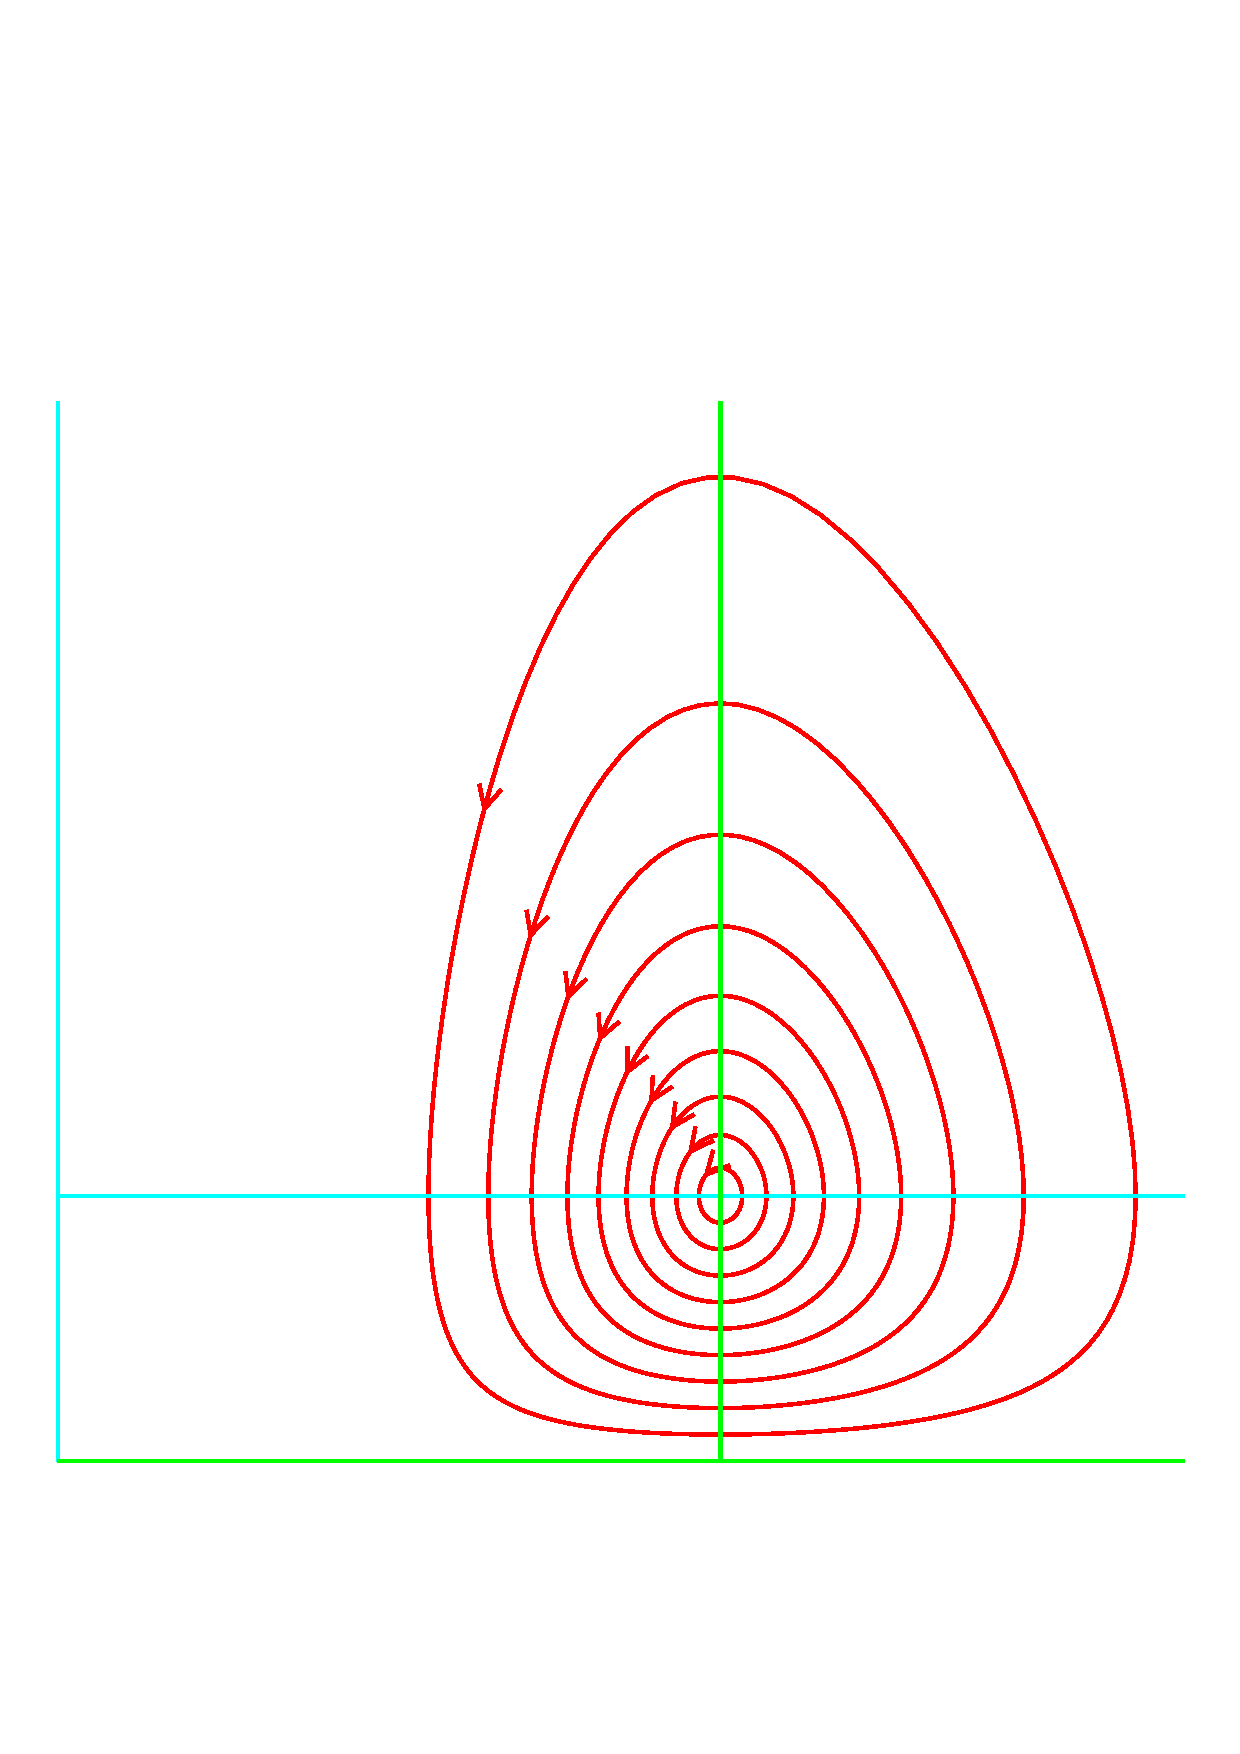
\includegraphics[scale=0.2]{images/lotka_volterra.pdf}};
   \draw (0.2,4.2) node{\includegraphics[scale=0.1]{images/shark.png}};
   \draw (4.3,0.3) node{\includegraphics[scale=0.1]{images/fish.png}};
   \draw (2.4,0.3) node[anchor=north]{$\ss \gm/\dl$};
   \draw (0.2,1.2) node[anchor=east]{$\ss \al/\bt$};
   \draw (6,3.5) node[anchor=west]{$\dot{F} = -\bt F(S-\al/\bt)$};
   \draw (6,3.0) node[anchor=west]{$\dot{S} = \dl S(F-\gm/\dl)$};
  \end{tikzpicture}
 \end{center}}
\end{frame}

\begin{frame}[t]
 \frametitle{Motion of a pendulum}
 
 \begin{tabular}{ll}
  \parbox[t]{7cm}{
   Consider a swinging pendulum, hanging at angle $\theta$. \\
   \uc<2->{The angular velocity \bhan{角速度} is $\om=\dot{\tht}$.}  \\
   \uc<3->{The angular acceleration \bhan{角加速度} $\dot{\om}$ is proportional to the component
   of the gravitational force perpendicular to the pendulum, which is
   proportional to $-\sin(\theta)$.}\\

   \uc<4->{With suitable units, we can assume that 
   \[ \uc<5->{\dot{\tht} = \om} \hspace{3em} \dot{\om}=-\sin(\tht). \]}

  } & \parbox[t]{4cm}{
   \begin{center}
    \begin{tikzpicture}
     \clip (0,-0.3) -- (4,-0.3) -- (4,3.6) -- (0,3.6) -- cycle;
     \draw (0,0) node[anchor=south west]{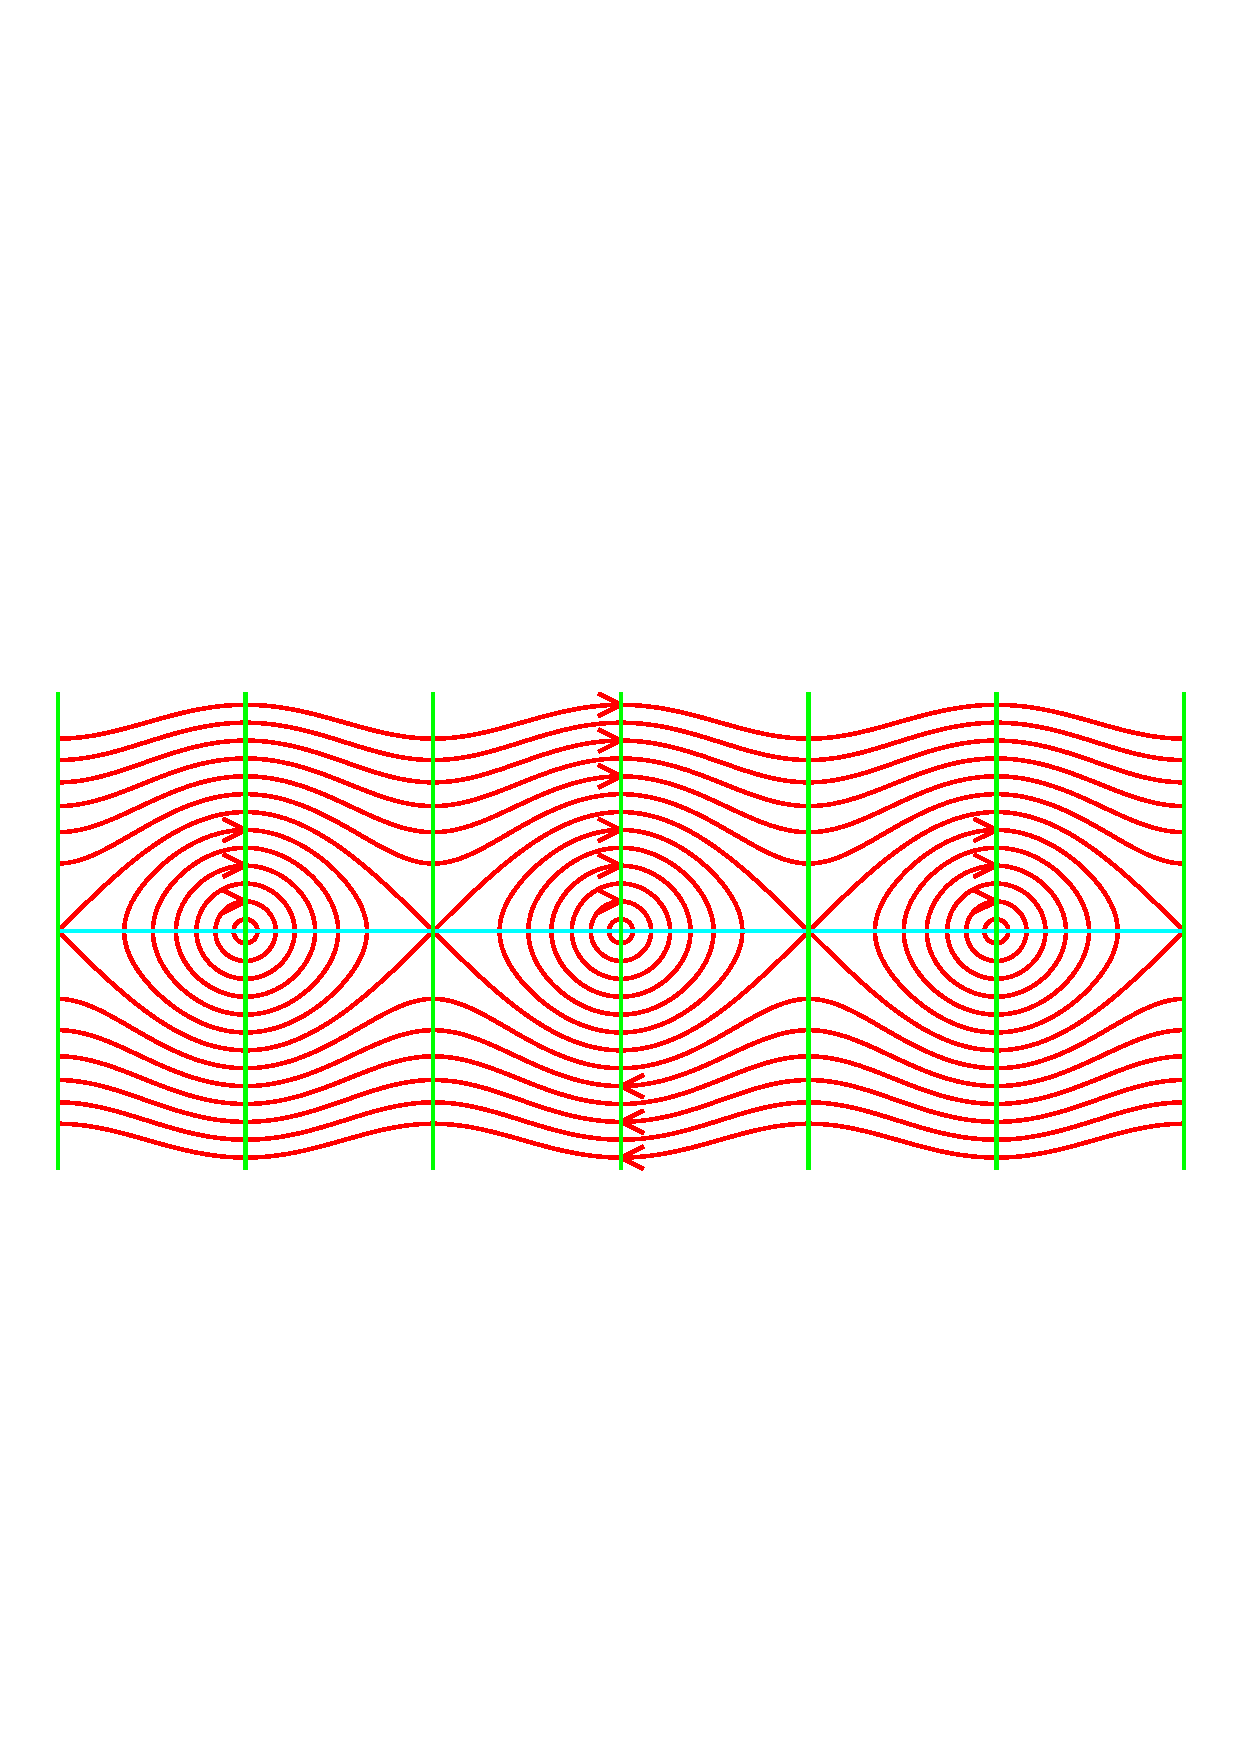
\includegraphics[scale=0.15,angle=30]{images/pendulum.png}};
     \begin{scope}[xshift=1.12cm,yshift=3.17cm]
      \draw (90:0.3) -- (270:3.5);    
      \draw (120:0.3) -- (300:2.4);
      \draw[thick,red] (0,0) (270:0.4) arc(270:300:0.4);
      \draw (285:0.6) node{$\ss\theta$};
      \begin{scope}[xshift=1.2cm,yshift=-2.4*0.866cm]
       \uc<3->{
       \draw[blue,->] (0,0) -- (270:1.2);
       \draw[blue,->] (0,0) -- (210:0.6);
       \draw[blue,dotted] (270:1.2) -- (210:0.6);}
      \end{scope}
     \end{scope}
    \end{tikzpicture}
   \end{center}
  }
 \end{tabular}

 \uc<6->{\[ 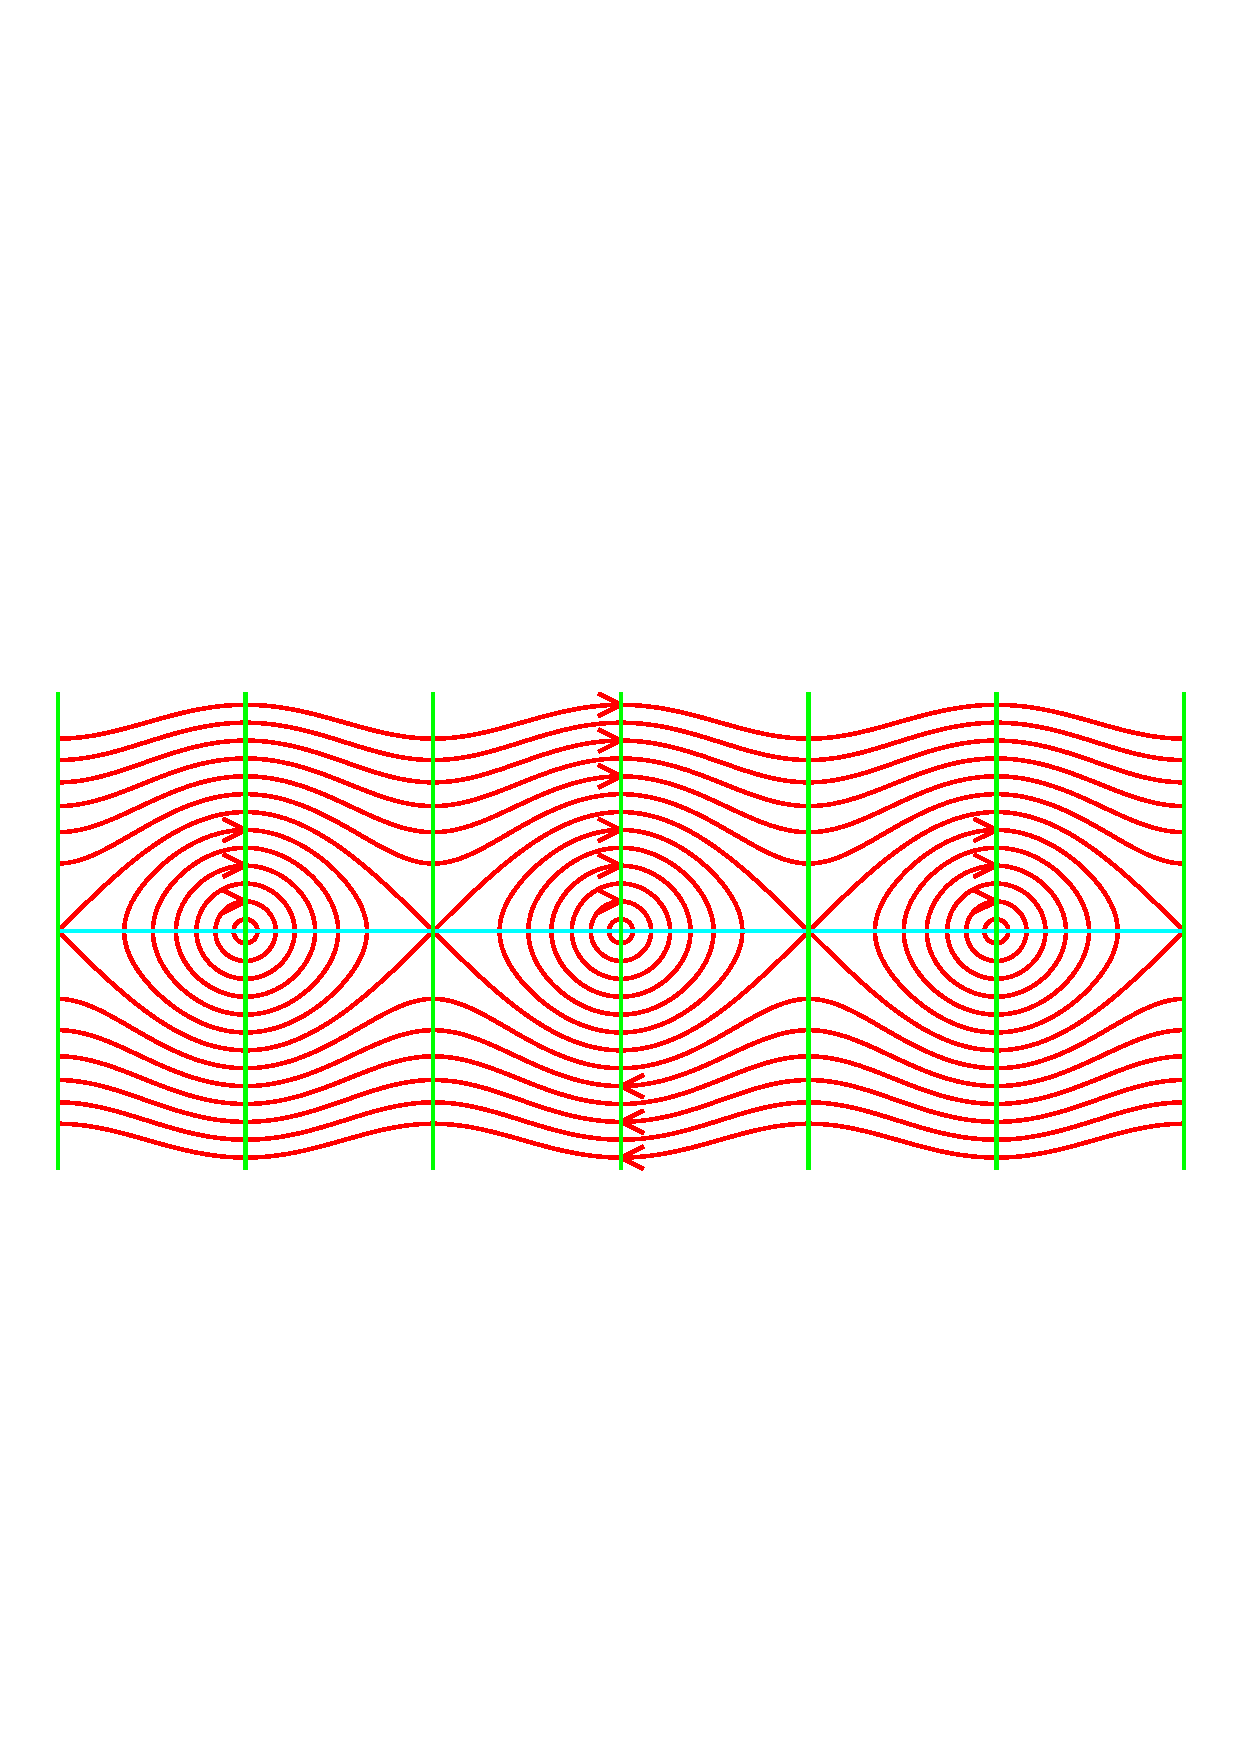
\includegraphics[scale=0.27,clip=true,trim=0cm 5cm 0cm 5cm]{images/pendulum.pdf} \]}
\end{frame}

\begin{frame}[t]
 \frametitle{A contour flow}
 
 This system has equations $\dot{x}=y^3-y$ and $\dot{y}=x-x^3$.
 \[ 
  \only<1| handout:0>{\includegraphics[scale=0.27]{images/contour_flow.pdf}}%
  \only<2| handout:0>{\includegraphics[scale=0.27]{images/contour_flow_xn.pdf}}%
  \only<3| handout:0>{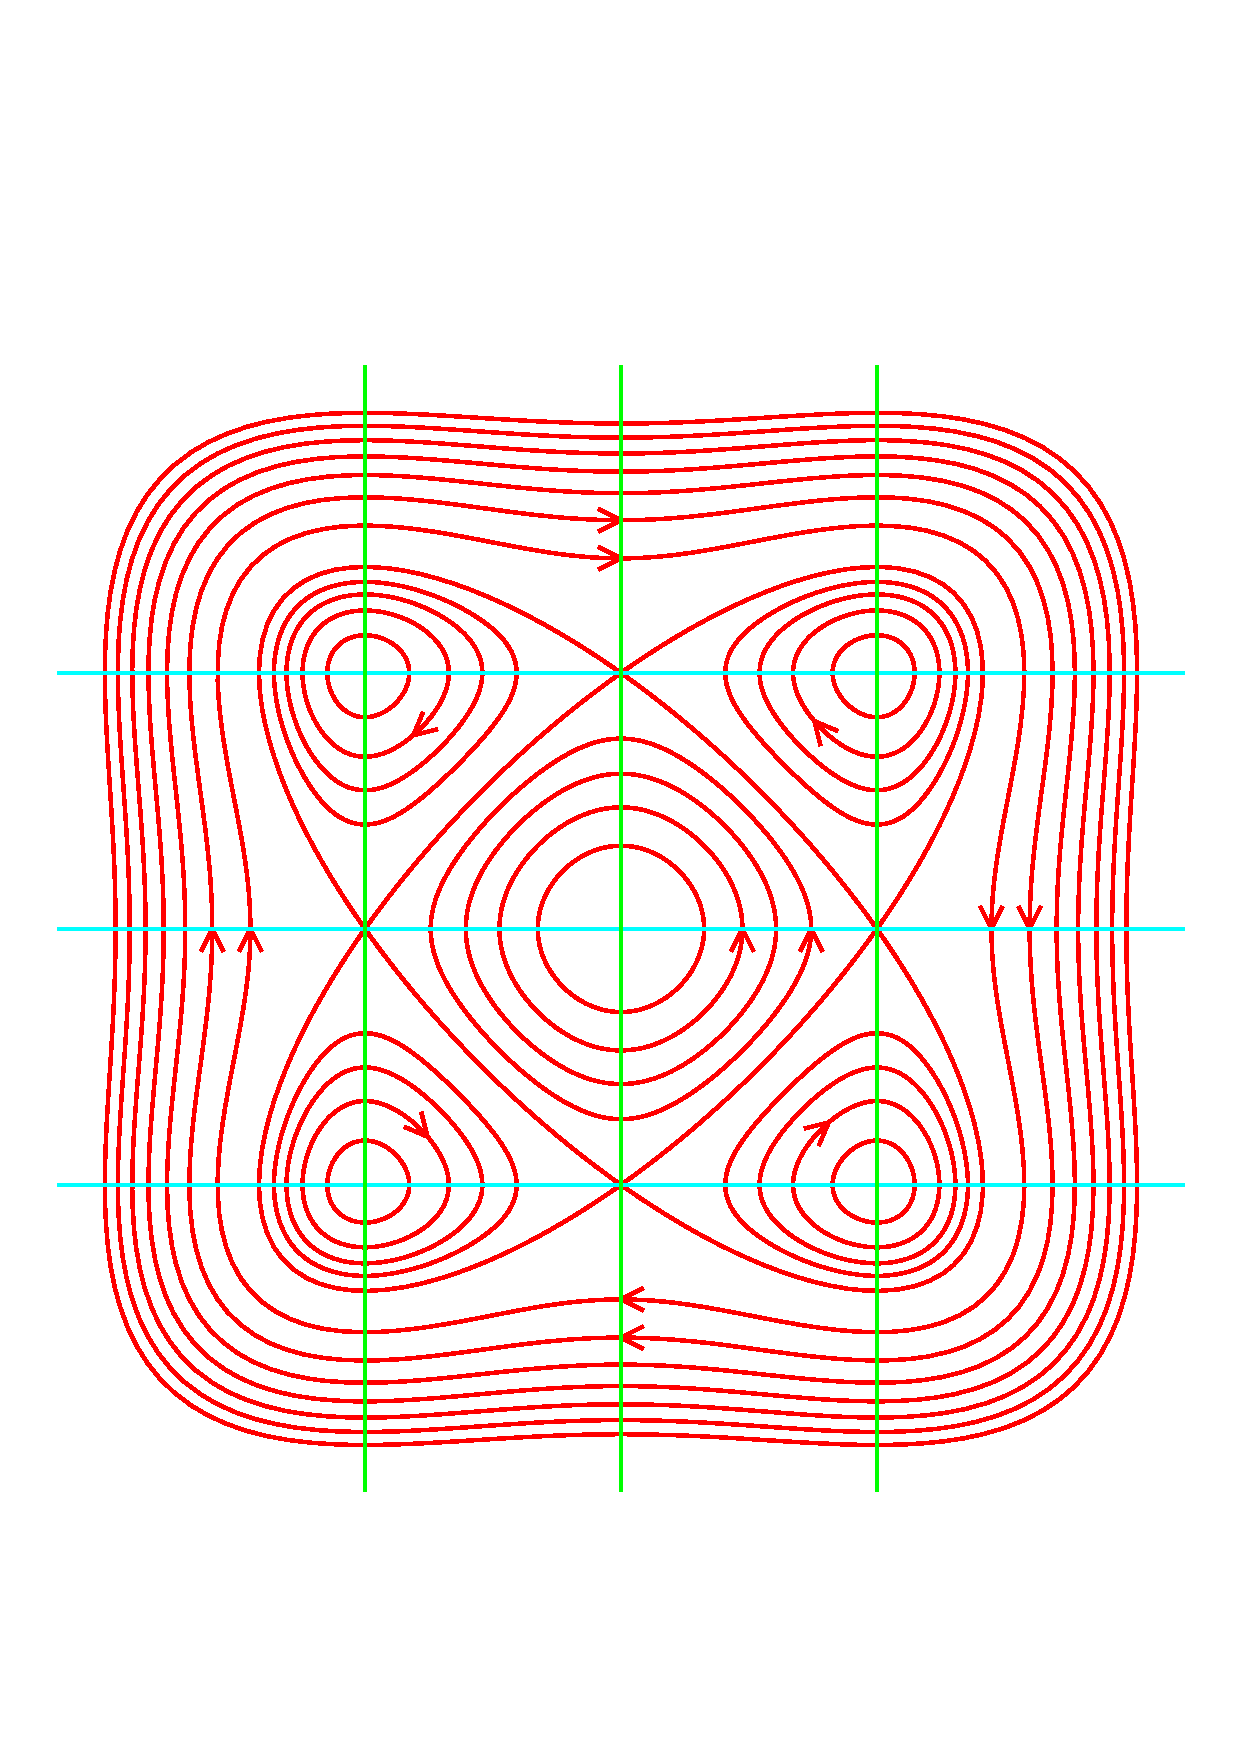
\includegraphics[scale=0.27]{images/contour_flow_xnyn.pdf}}%
  \only<4->{\includegraphics[scale=0.27]{images/contour_flow_xnynep.pdf}}
 \]
 \vspace{-4ex}
 \begin{itemize}
  \item<2-> The blue lines (\emph{$x$-nullclines}) show where $y-y^3=0$ and so $\dot{x}=0$.
  \item<3-> The green lines (\emph{$y$-nullclines}) show where $x-x^3=0$ and so $\dot{y}=0$.
  \item<4-> The black dots (\emph{equilibrium points}) show where $\dot{x}=\dot{y}=0$.
 \end{itemize}
\end{frame}

\begin{frame}[t]
 \frametitle{A contour map}
 
 \[ \includegraphics[scale=0.7]{images/contour_map_small.jpg} \]
 This is a contour map.  The height is $h(x,y)$.  If you stay on one
 of the brown lines (contours), then you stay at the same height.  
 That is a contour flow.
\end{frame}

\begin{frame}[t]
 \frametitle{A contour map}
 
 \[ \includegraphics[scale=0.55]{images/explain_contours.jpg} \]
 When the contours are close together, the ground is steep.  \\
 When the contours are far apart, the ground is not steep.
\end{frame}

\begin{frame}[t]
 \frametitle{A gradient flow}
 
 This system has equations $\dot{x}=x-x^3$ and $\dot{y}=y-y^3$.
 \[ 
  \only<1| handout:0>{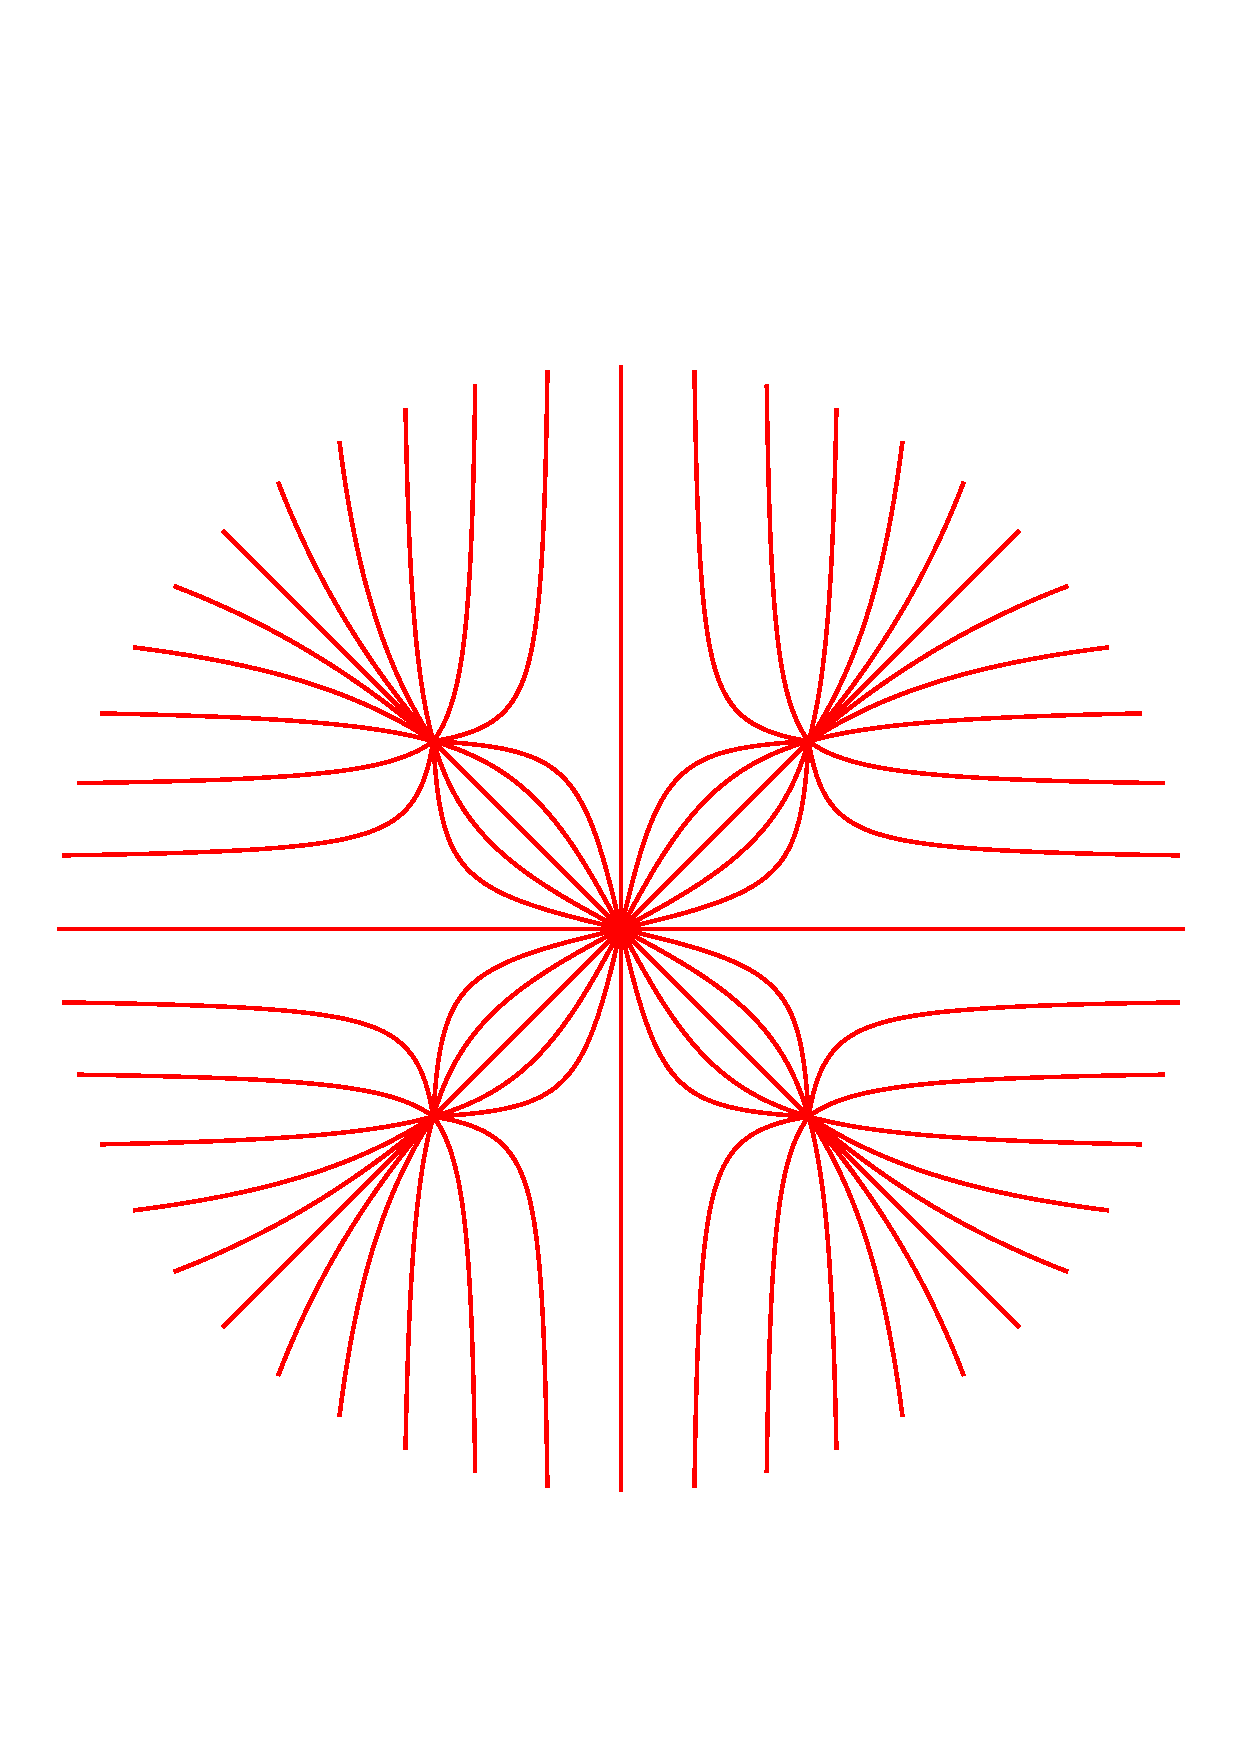
\includegraphics[scale=0.27]{images/gradient_flow.pdf}}%
  \only<2| handout:0>{\includegraphics[scale=0.27]{images/gradient_flow_xn.pdf}}%
  \only<3| handout:0>{\includegraphics[scale=0.27]{images/gradient_flow_xnyn.pdf}}%
  \only<4->{\includegraphics[scale=0.27]{images/gradient_flow_xnynep.pdf}}
 \]
 \vspace{-4ex}
 \begin{itemize}
  \item<2-> The blue lines (\emph{$x$-nullclines}) show where $x-x^3=0$ and so $\dot{x}=0$.
  \item<3-> The green lines (\emph{$y$-nullclines}) show where $y-y^3=0$ and so $\dot{y}=0$.
  \item<4-> The black dots (\emph{equilibrium points}) show where $\dot{x}=\dot{y}=0$.
 \end{itemize}
\end{frame}

\begin{frame}<handout:0>[t]
%\begin{frame}[t]
 \frametitle{Question: which is the $y$-nullcline?}
 
 Which of the curves below is the $y$-nullcline?

 \[
  \only<1| handout:0>{\includegraphics[scale=0.3]{images/find_y_nullcline_a.pdf}}%
  \only<2>{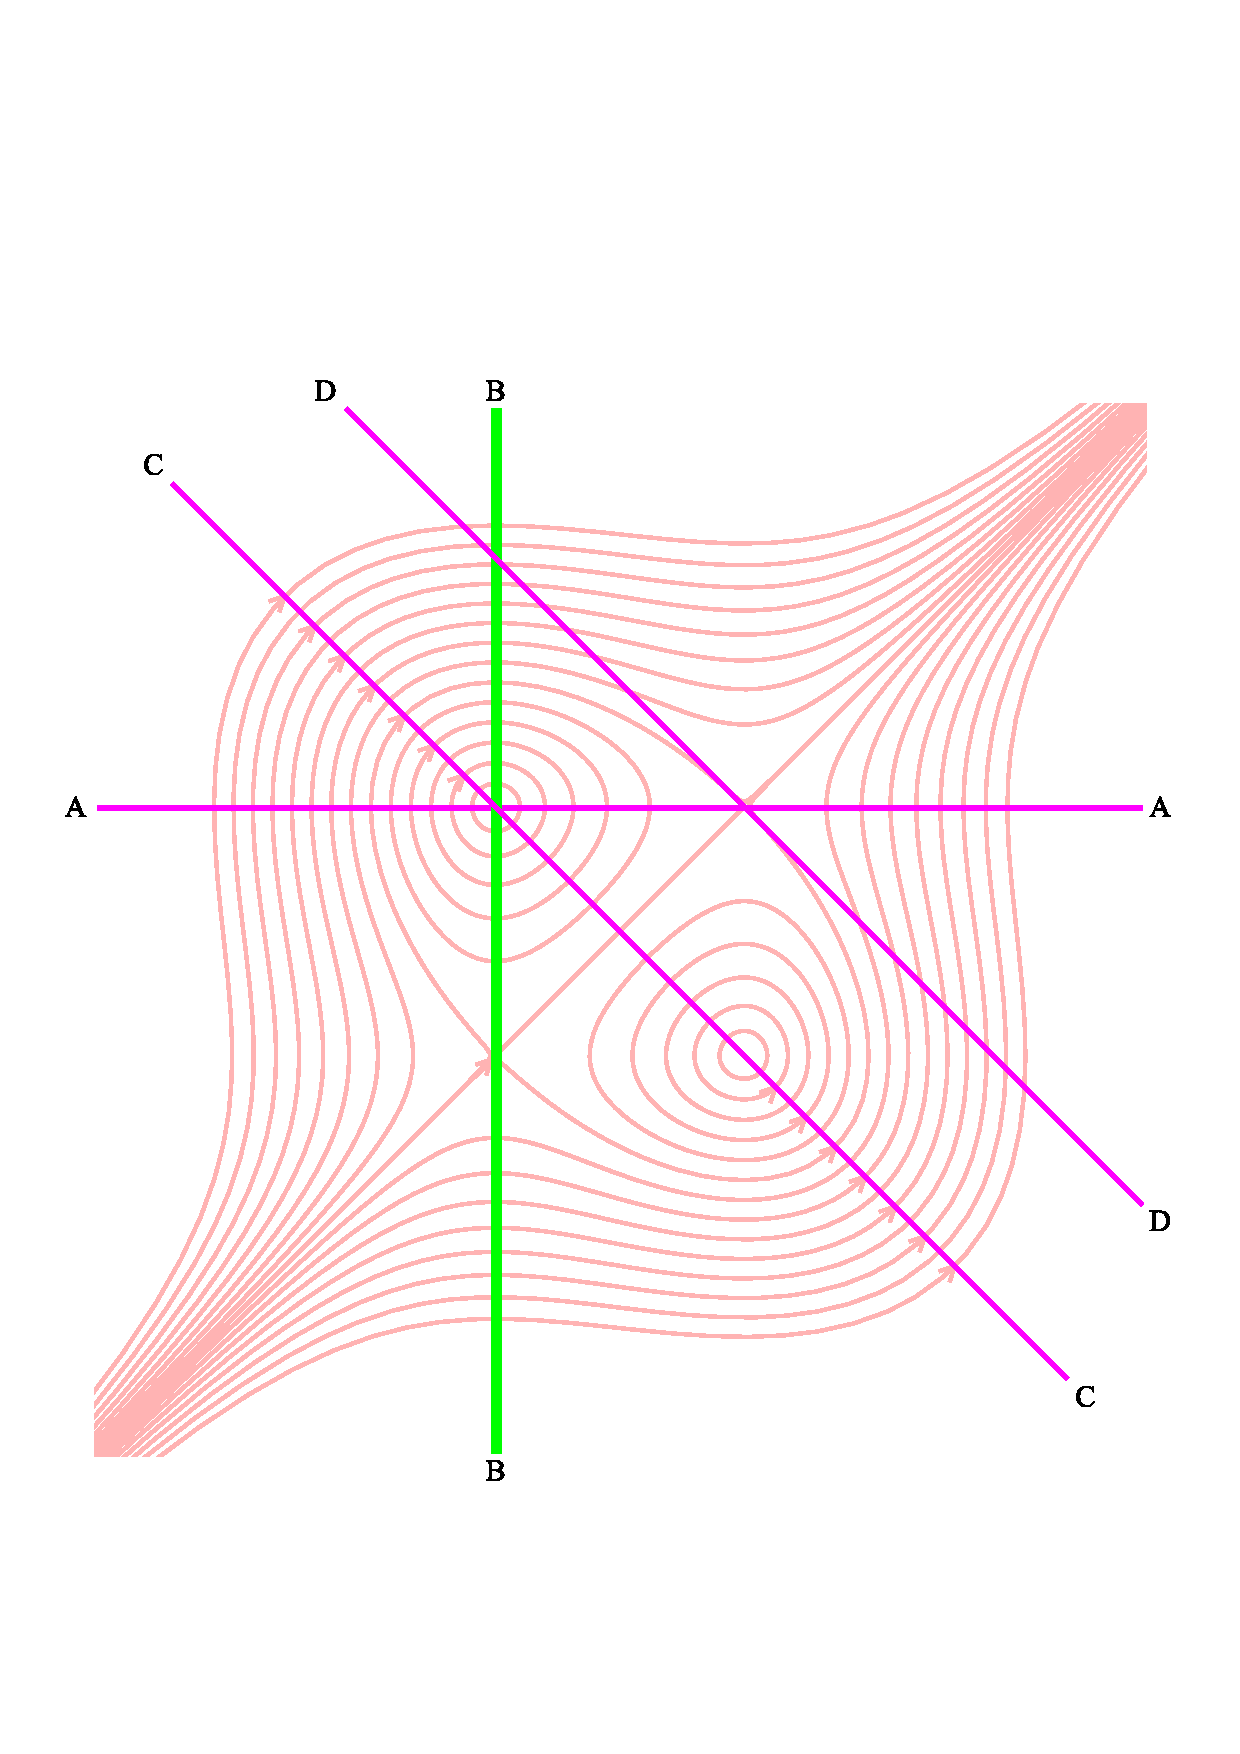
\includegraphics[scale=0.3]{images/find_y_nullcline_ans_a.pdf}}%
 \]
 \uc<2->{
  Curve B is the $y$-nullcline; the flow lines cross it horizontally, with $\dot{y}=0$.
 }
\end{frame}

\begin{frame}<handout:0>[t]
%\begin{frame}[t]
 \frametitle{Question: how many equilibria?}
 
 How many equilibrium points are there in this phase portrait?
 \[ 
   \only<1| handout:0>{\includegraphics[scale=0.3]{images/misc_c.pdf}}%
   \only<2->{\includegraphics[scale=0.3]{images/misc_c_1.pdf}}%
 \]
 \uc<2->{There are two equilibrium points, as shown.}
\end{frame}

\begin{frame}[t]
 \frametitle{Bands}
 
 This system has equations $\dot{x}=1$ and $\dot{y}=\sin(\pi y)$.
 \[ 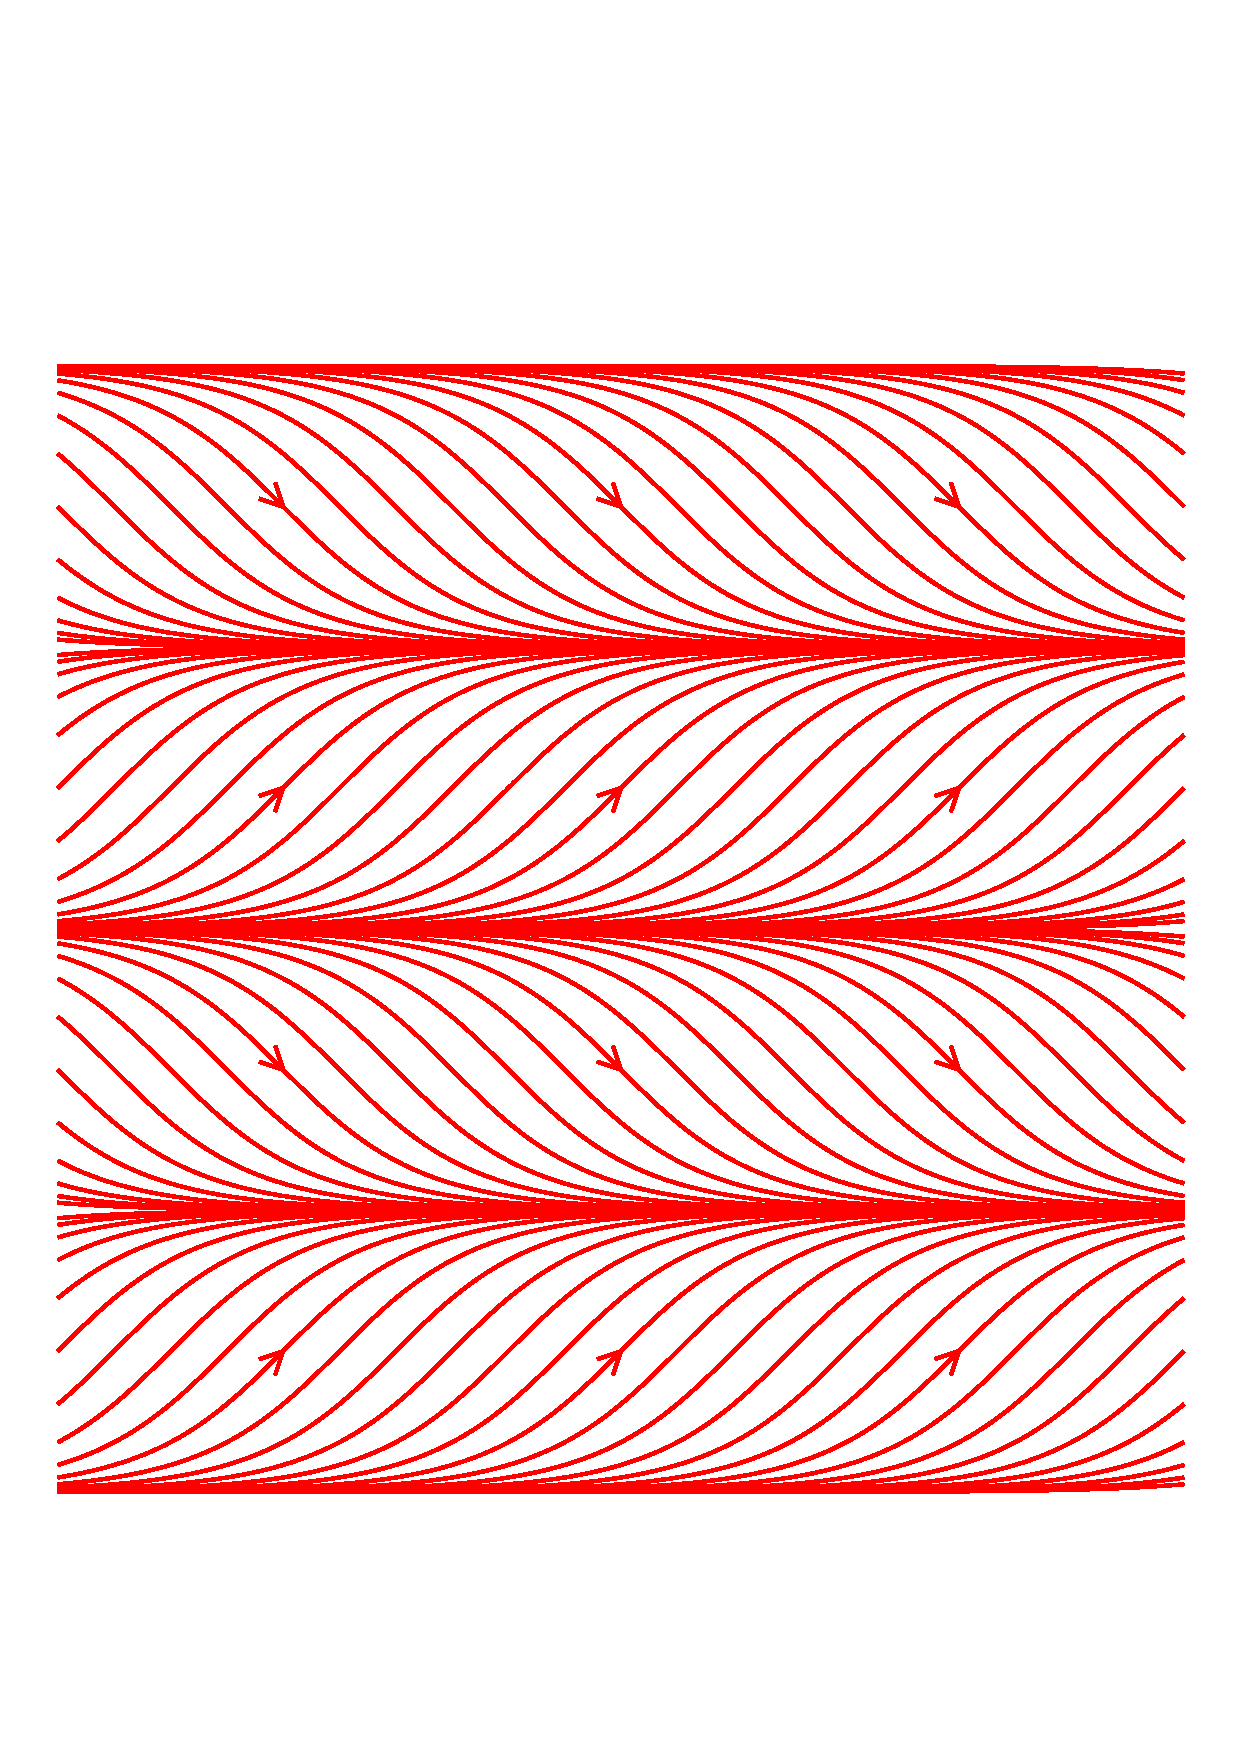
\includegraphics[scale=0.27]{images/bands.pdf} \]

 The solutions move steadily to the right, and converge to one of the lines 
 where $y$ is an odd integer.
\end{frame}

\begin{frame}[t]
 \frametitle{Duffing oscillator}
 
 The Duffing oscillator \bhan{振荡器} has $\dot{x}=y$ and $\dot{y}=2x-x^3$.
 \[ 
  \only<1| handout:0>{\includegraphics[scale=0.25]{images/duffing.pdf}}%
  \only<2| handout:0>{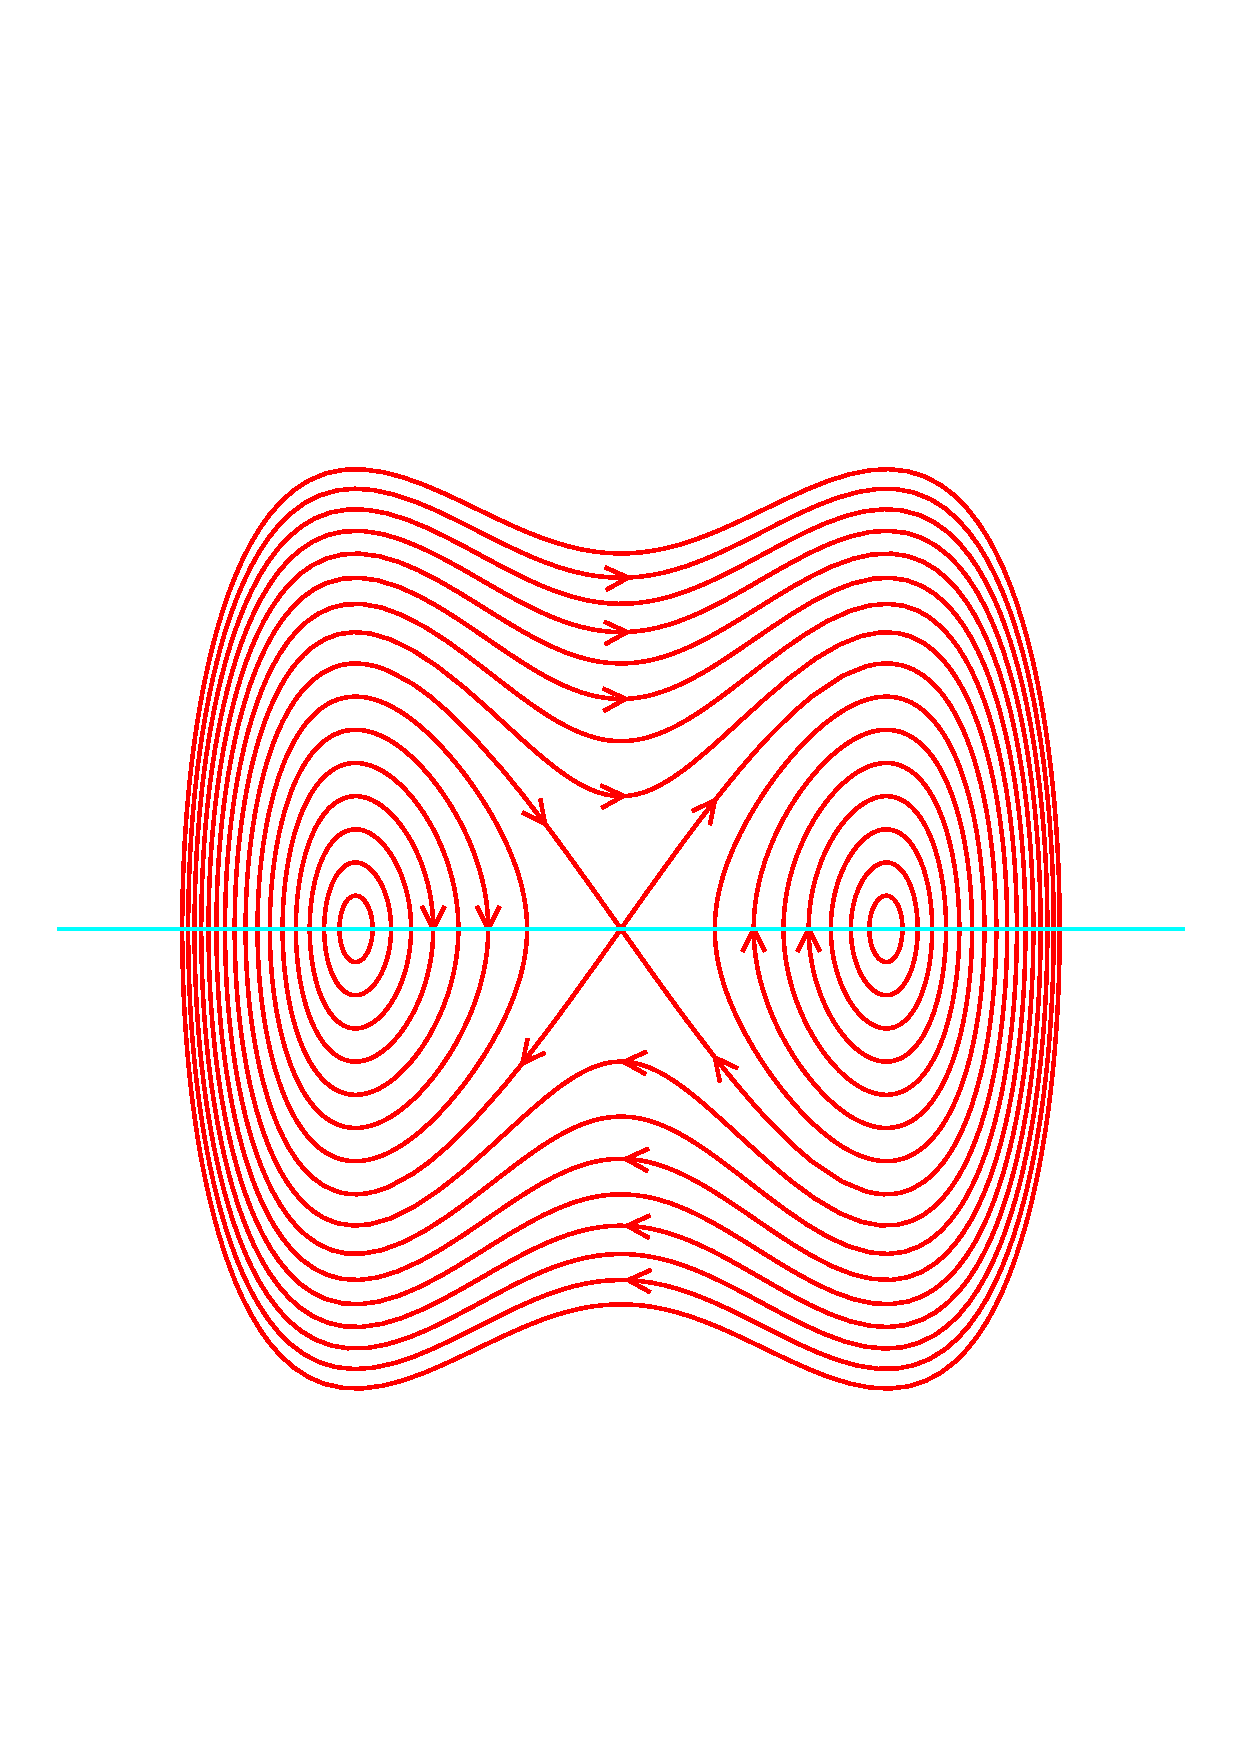
\includegraphics[scale=0.25]{images/duffing_xn.pdf}}%
  \only<3| handout:0>{\includegraphics[scale=0.25]{images/duffing_xnyn.pdf}}%
  \only<4->{\includegraphics[scale=0.25]{images/duffing_xnynep.pdf}}
 \]
 \vspace{-4ex}
 \begin{itemize}
  \item<2-> The blue line (\emph{$x$-nullcline}) shows where $y=0$ and so $\dot{x}=0$.
  \item<3-> The green lines (\emph{$y$-nullclines}) show where $2x-x^3=0$ and so $\dot{y}=0$.
  \item<4-> The black dots (\emph{equilibrium points}) show where $\dot{x}=\dot{y}=0$.
 \end{itemize}
\end{frame}

\begin{frame}[t]
 \frametitle{Damped Duffing oscillator}
 
 This system has $\dot{x}=y$ and $\dot{y}=2x-x^3-0.1y$.
 \[ 
  \only<1| handout:0>{\includegraphics[scale=0.25]{images/damped_duffing.pdf}}%
  \only<2| handout:0>{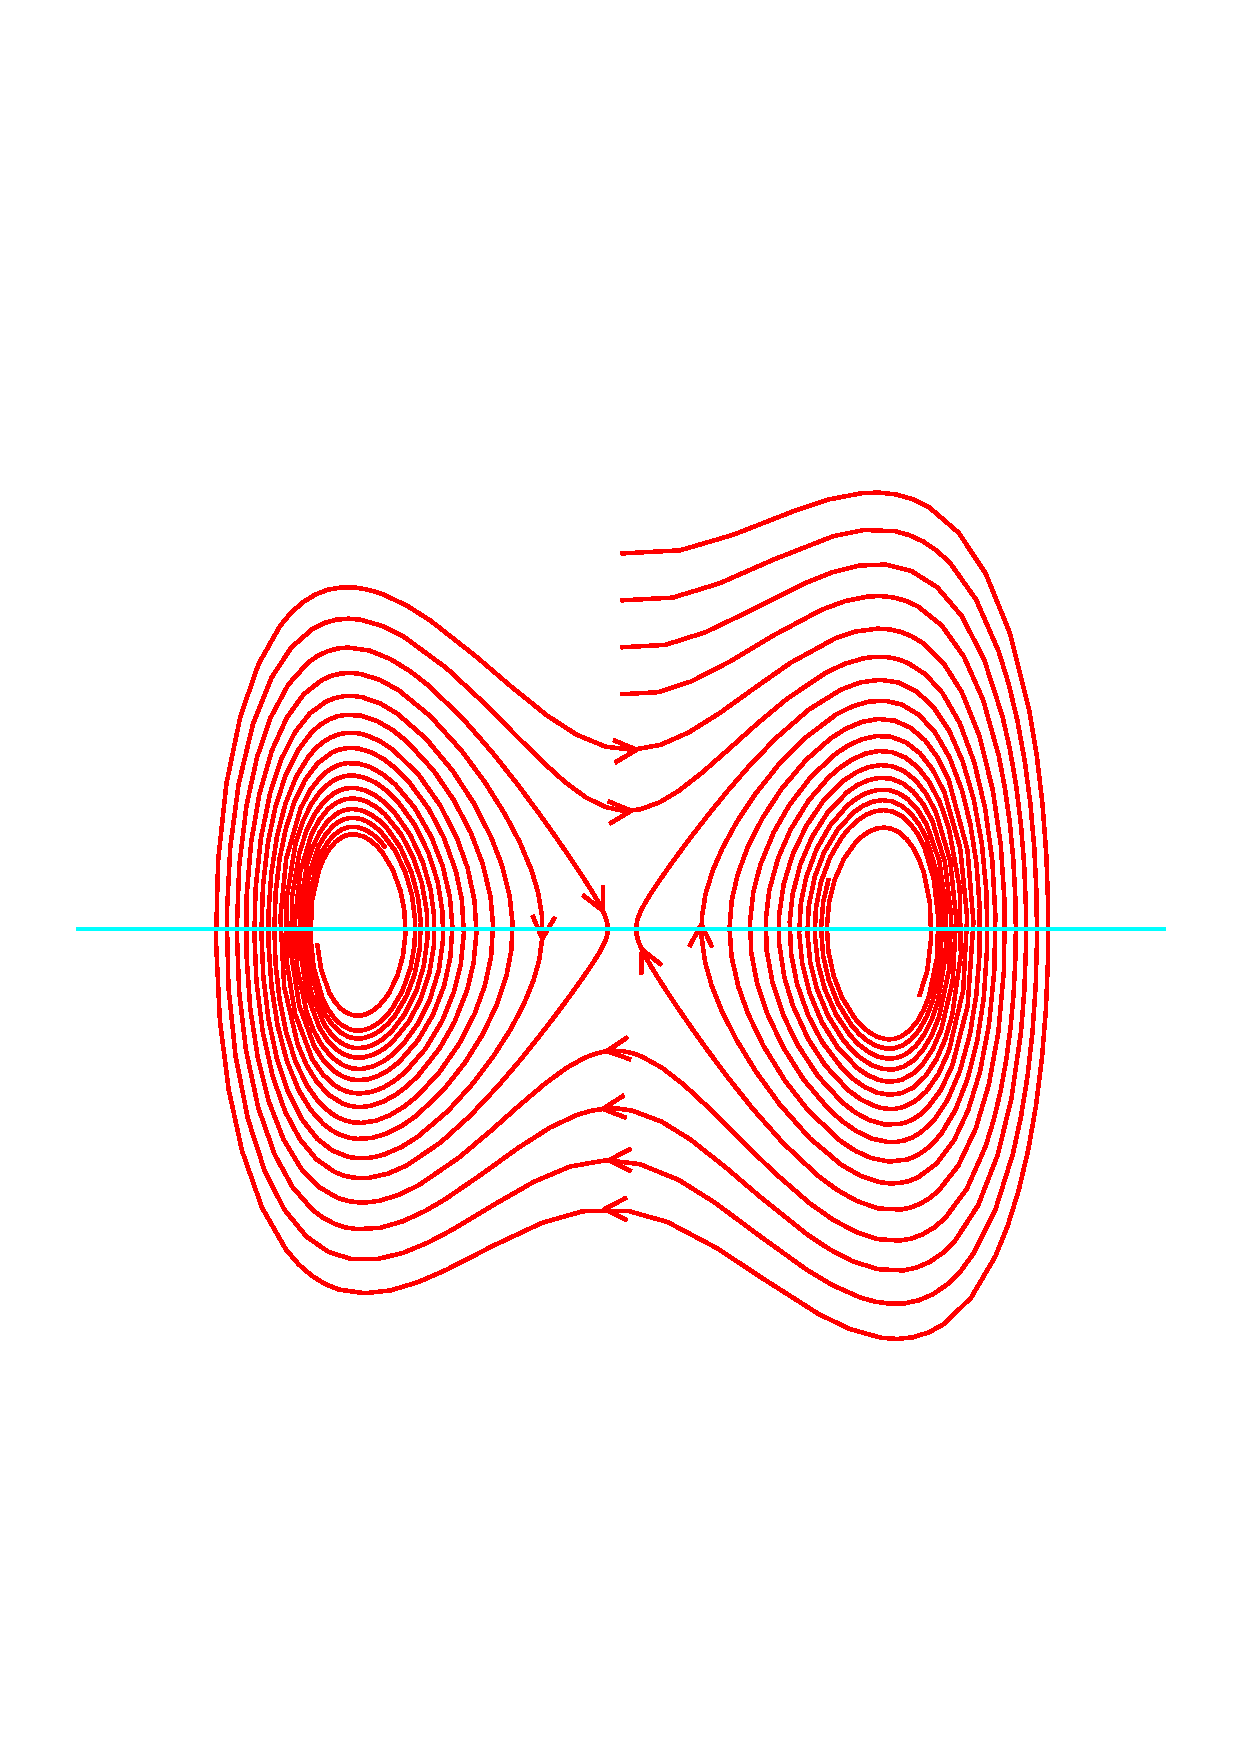
\includegraphics[scale=0.25]{images/damped_duffing_xn.pdf}}%
  \only<3| handout:0>{\includegraphics[scale=0.25]{images/damped_duffing_xnyn.pdf}}%
  \only<4->{\includegraphics[scale=0.25]{images/damped_duffing_xnynep.pdf}}
 \]
 \vspace{-4ex}

 It is similar to the Duffing oscillator, but with friction or damping \bhan{内耗}.

 \begin{itemize}
  \item<2-> The $x$-nullcline is the same as before
  \item<3-> But the $y$-nullclines have moved slightly
  \item<4-> The equilibrium points are unchanged.
 \end{itemize}
\end{frame}

\begin{frame}<handout:0>[t]
%\begin{frame}[t]
 \frametitle{Question: which is the $y$-nullcline?}
 
 Which of the curves below is the $y$-nullcline?

 \[
  \only<1| handout:0>{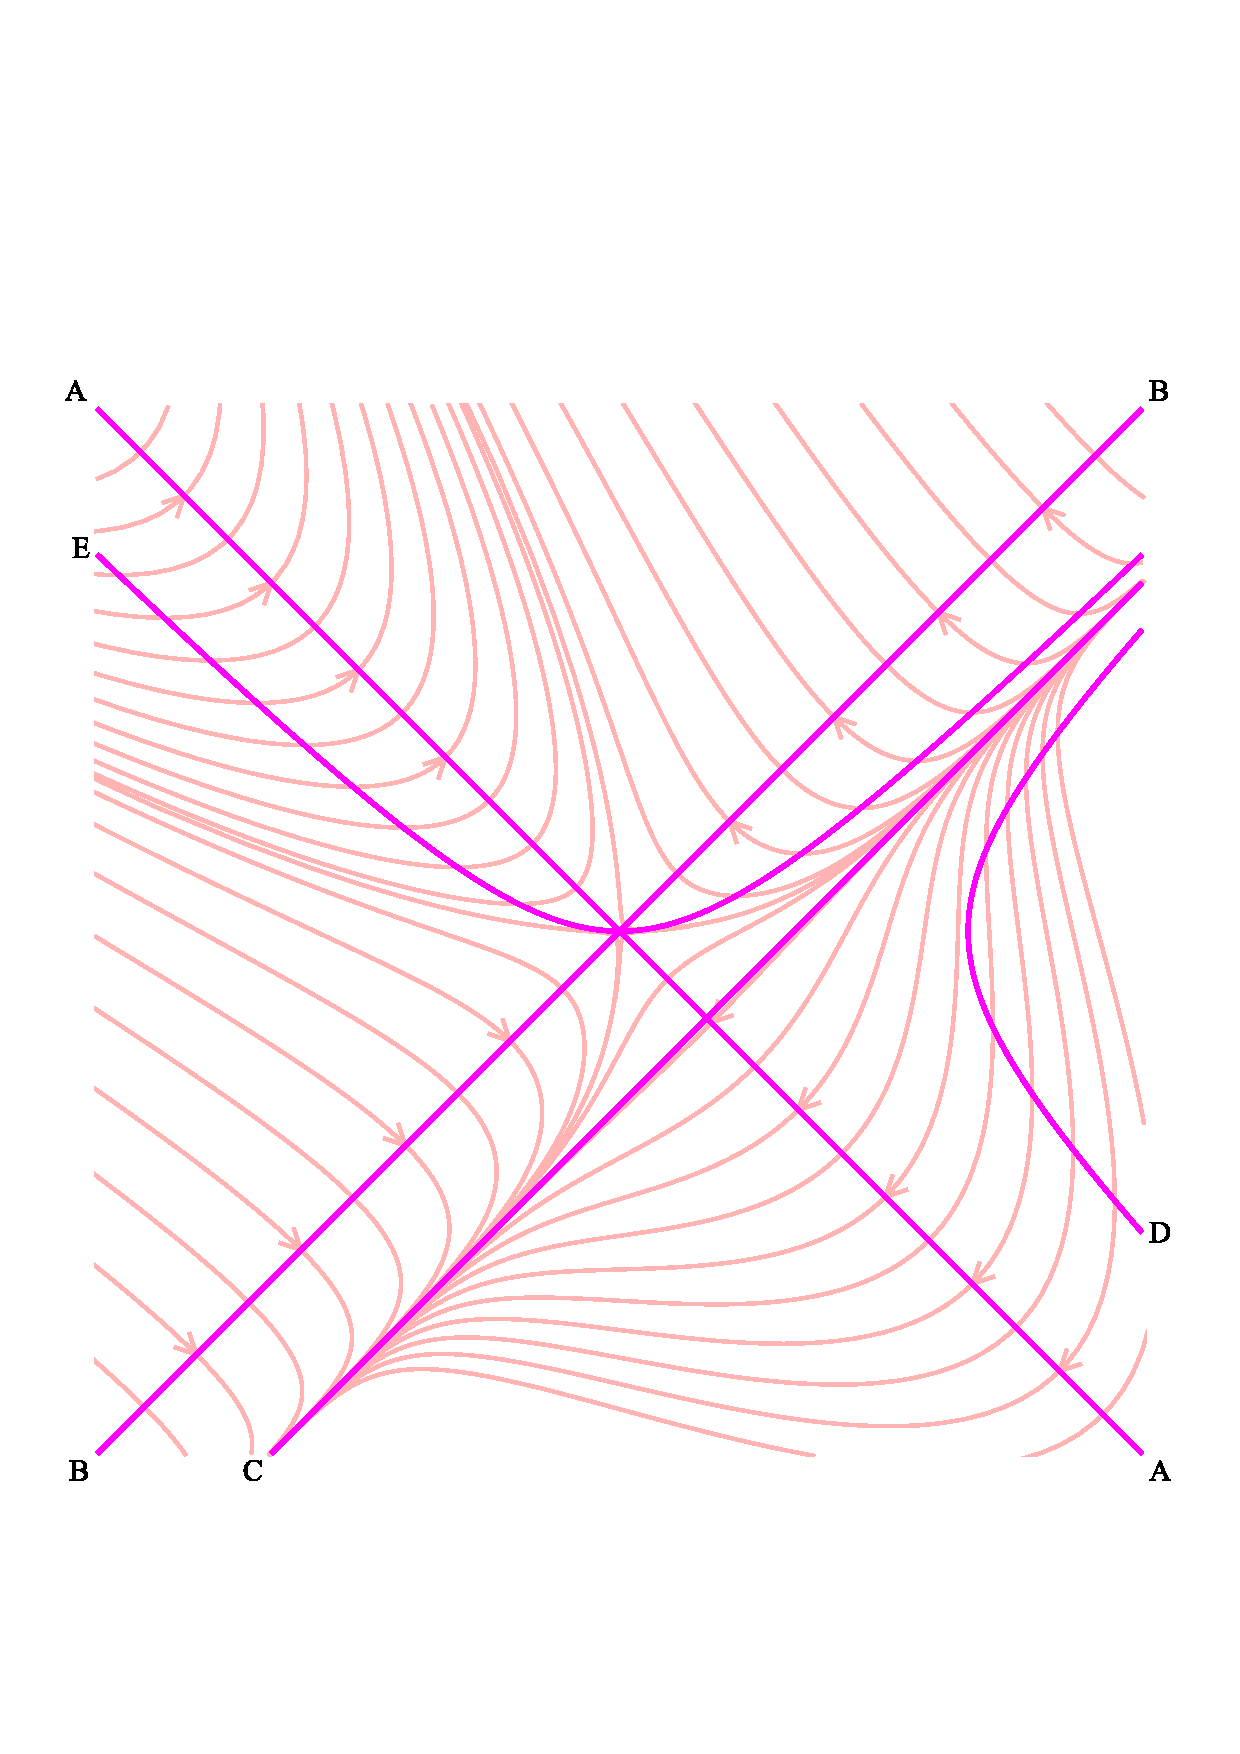
\includegraphics[scale=0.3]{images/find_y_nullcline_b.pdf}}%
  \only<2>{\includegraphics[scale=0.3]{images/find_y_nullcline_ans_b.pdf}}%
 \]
 \uc<2->{
  Curve E is the $y$-nullcline; the flow lines cross it horizontally, with $\dot{y}=0$.
 }
\end{frame}

\begin{frame}[t]
 \frametitle{van der Pol oscillator}
 
 This system has $\dot{x}=y$ and $\dot{y}=2(1-x^2)y - x$.
 \[ 
  \only<1| handout:0>{\includegraphics[scale=0.25]{images/van_der_pol.pdf}}%
  \only<2| handout:0>{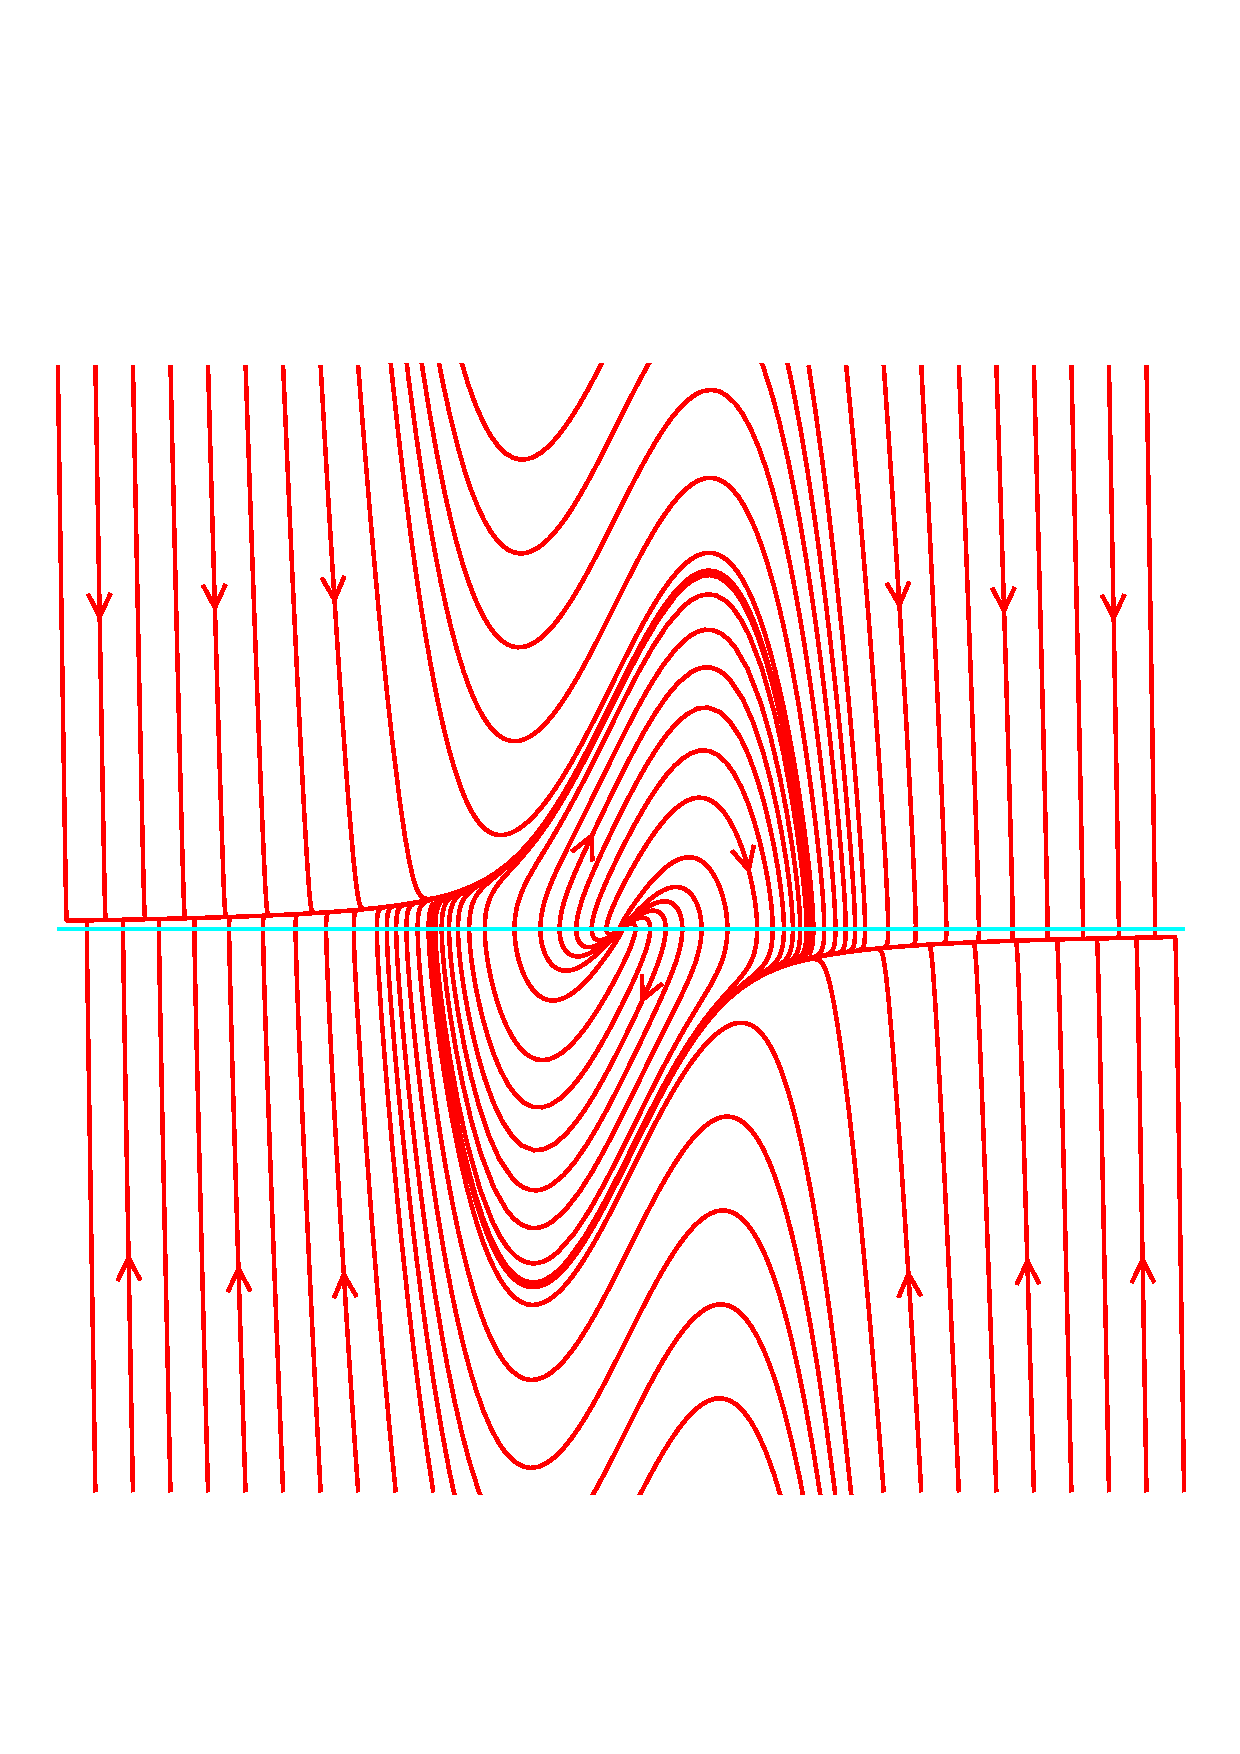
\includegraphics[scale=0.25]{images/van_der_pol_xn.pdf}}%
  \only<3| handout:0>{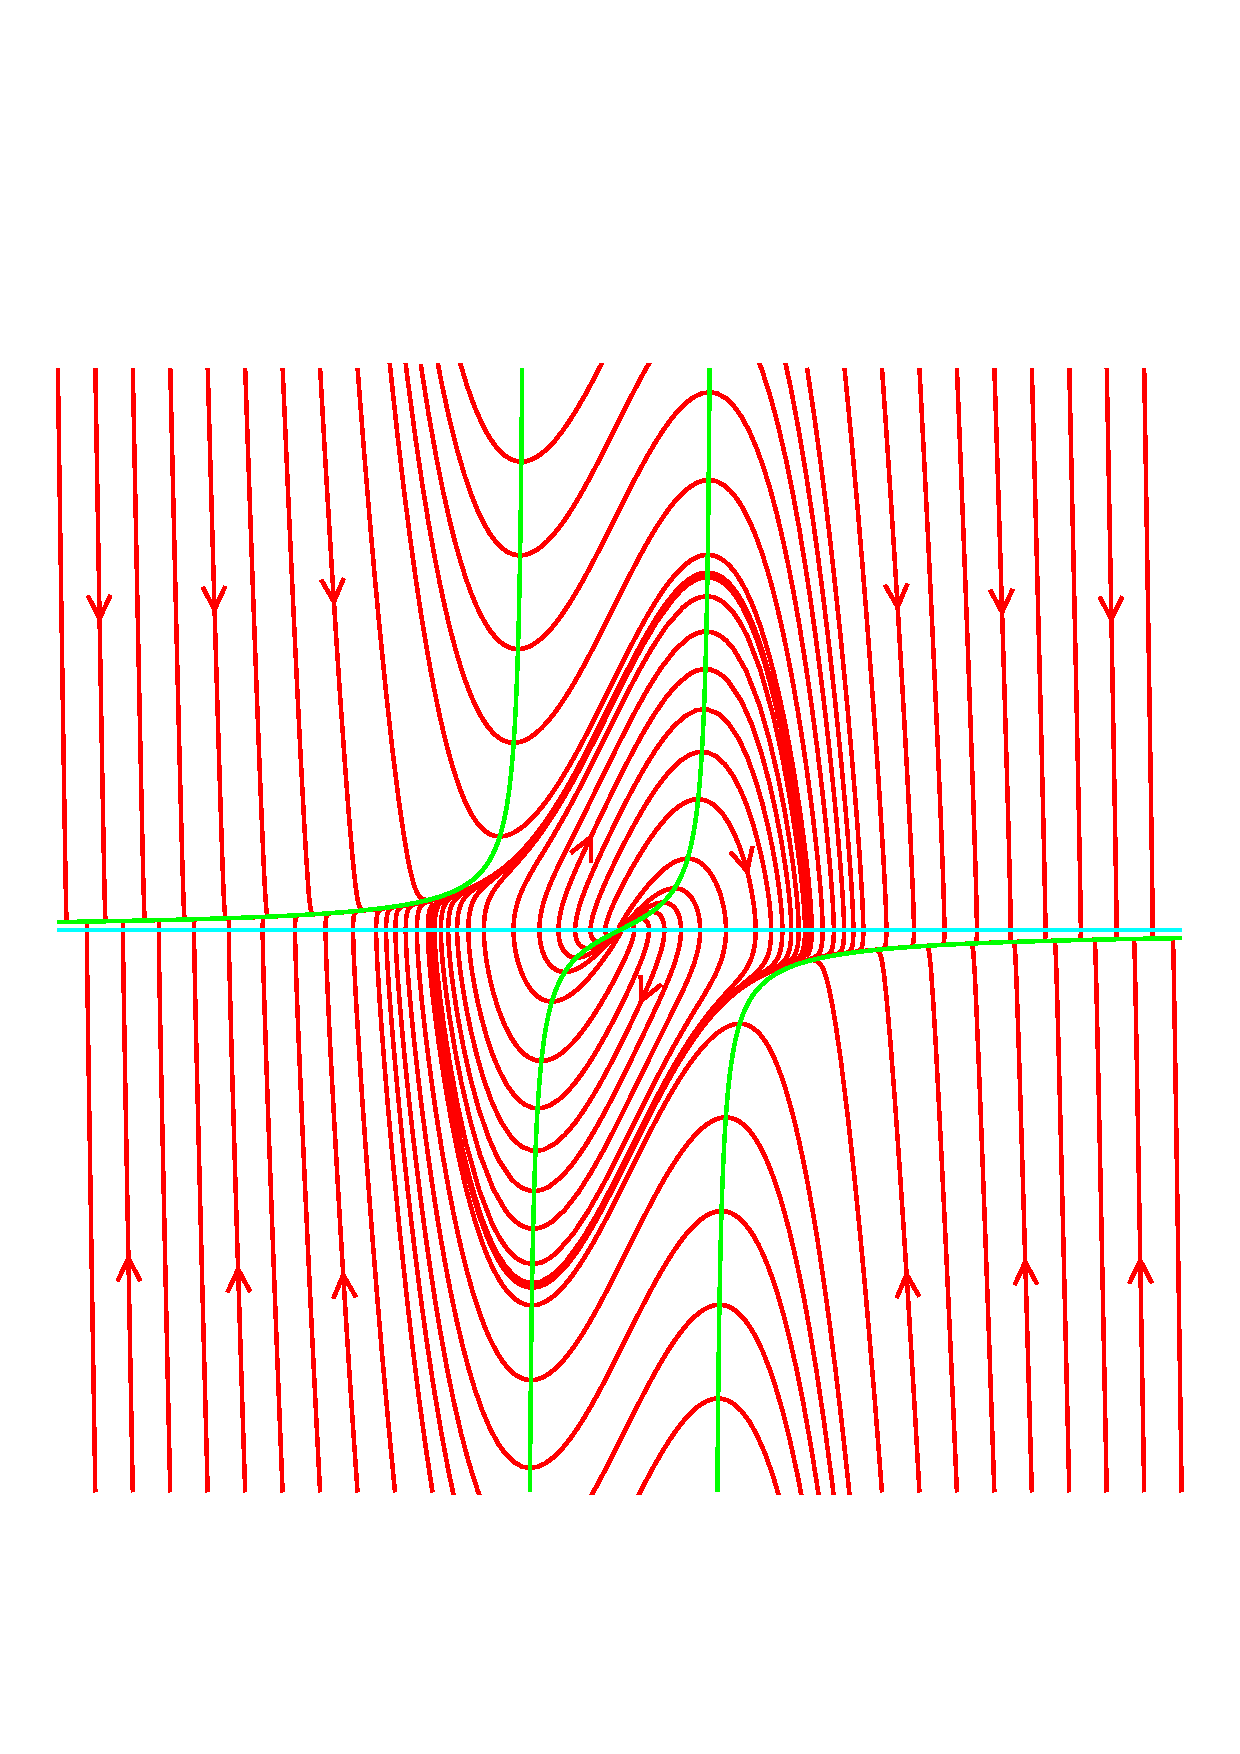
\includegraphics[scale=0.25]{images/van_der_pol_xnyn.pdf}}%
  \only<4->{\includegraphics[scale=0.25]{images/van_der_pol_xnynep.pdf}}
 \]
 \vspace{-4ex}
 \begin{itemize}
  \item<2-> The blue line (\emph{$x$-nullcline}) shows where $y=0$ and so $\dot{x}=0$.
  \item<3-> The green lines (\emph{$y$-nullclines}) show where $2(1-x^2)y-x=0$ and so $\dot{y}=0$.
  \item<4-> There is only one equilibrium point, but there is also a \emph{limit cycle},
            shown in blue.  All non-constant solutions converge to the limit cycle.
 \end{itemize}
\end{frame}

\begin{frame}[t]
 \frametitle{Sketching a phase portrait}
 We will sketch the phase portrait for the system $\dot{x}=x(3-x-2y),\;\dot{y}=y(x-1)$.
 \begin{center}
  \begin{tikzpicture}
   \draw[white] (-1.5,-2.5) -- (5.5,3.5);
   \only<13-> { 
    \draw(2,0.507) node{\includegraphics[scale=0.315,clip=true,trim=1cm 1cm 1cm 1cm]{images/predator_faded.pdf}};
   }
   \only<2-3| handout:0>{
    \draw[cyan] (-1,2) -- (5,-1);
    \draw[cyan] (0,-2) -- (0,3);
   }
   \only<3| handout:0>{
    \draw( 2.0, 1.5) node{$\ss\dot{x}<0$};
    \draw(-0.5, 2.5) node{$\ss\dot{x}>0$};
    \draw(-0.5,-1.0) node{$\ss\dot{x}<0$};
    \draw( 2.0,-1.0) node{$\ss\dot{x}>0$};
   }
   \only<4->{
    \draw[green] (-1,0) -- (5,0);
    \draw[green] (1,-2) -- (1,3);
   }
   \only<5-9| handout:0>{
    \draw(-0.5, 2.1) node{$\ss\dot{y}<0$};
    \draw( 2.0, 2.1) node{$\ss\dot{y}>0$};
    \draw( 2.0,-1.3) node{$\ss\dot{y}<0$};
    \draw(-0.5,-1.3) node{$\ss\dot{y}>0$};
   }
   \uc<6->{
    \draw[cyan] (-1,2) -- (5,-1);
    \draw[cyan] (0,-2) -- (0,3);
   }
   \uc<7->{
    \fill[black] (0,0) circle(0.05);
    \fill[black] (3,0) circle(0.05);
    \fill[black] (1,1) circle(0.05);
   }
   \only<8-9| handout:0>{
    \draw( 2.0, 1.5) node{$\ss\dot{x}<0$};
    \draw(-0.5, 2.5) node{$\ss\dot{x}>0$};
    \draw(-0.5,-1.0) node{$\ss\dot{x}<0$};
    \draw( 2.0,-1.0) node{$\ss\dot{x}>0$};
    \draw( 0.5, 2.1) node{$\ss\dot{x}<0$};
    \draw( 0.5, 0.6) node{$\ss\dot{x}>0$};
    \draw( 0.5,-1.0) node{$\ss\dot{x}>0$};
    \draw(-0.5, 0.8) node{$\ss\dot{x}<0$};
    \draw( 1.5, 0.4) node{$\ss\dot{x}>0$};
    \draw( 4.2,-0.3) node{$\ss\dot{x}<0$};
   }
   \only<9| handout:0>{
    \draw(-0.5, 0.5) node{$\ss\dot{y}<0$};
    \draw( 0.5, 1.8) node{$\ss\dot{y}<0$};
    \draw( 0.5, 0.3) node{$\ss\dot{y}<0$};
    \draw( 0.5,-1.3) node{$\ss\dot{y}>0$};
    \draw( 2.1, 0.2) node{$\ss\dot{y}>0$};
    \draw( 4.7,-0.6) node{$\ss\dot{y}<0$};
   }
   \uc<10->{
    \draw[orange,->] (-0.5, 2.5) -- +(- 45:0.3);
    \draw[orange,->] (-0.5, 0.8) -- +(-135:0.3);
    \draw[orange,->] (-0.5,-1.0) -- +( 135:0.3);
    \draw[orange,->] ( 0.5, 2.1) -- +(-135:0.3);
    \draw[orange,->] ( 0.5, 0.6) -- +(- 45:0.3);
    \draw[orange,->] ( 0.5,-1.0) -- +(  45:0.3);
    \draw[orange,->] ( 2.5, 2.0) -- +( 135:0.3);
    \draw[orange,->] ( 1.6, 0.2) -- +(  45:0.3);
    \draw[orange,->] ( 2.5,-1.0) -- +( -45:0.3);
    \draw[orange,->] ( 4.5,-0.3) -- +(-135:0.3);
   }
   \uc<11->{
    \draw[red] (0,3) -- (0,-2);
    \draw[red,->] (0,3) -- (0,2.25);
    \draw[red,->] (0,1.5) -- (0,0.75);
    \draw[red,->] (0,-2) -- (0,-1);
    \foreach \x in {-1,-0.9,...,0.8} {
     \draw[red] ({\x},{1.5-0.5*\x-0.05}) -- ({\x},{1.5-0.5*\x+0.05});
    }
    \foreach \x in {1.3,1.4,...,2.8} {
     \draw[red] ({\x},{1.5-0.5*\x-0.05}) -- ({\x},{1.5-0.5*\x+0.05});
    }
    \foreach \x in {3.3,3.4,...,5} {
     \draw[red] ({\x},{1.5-0.5*\x-0.05}) -- ({\x},{1.5-0.5*\x+0.05});
    }
   }
   \uc<12->{
    \draw[red] (-1,0) -- (5,0);
    \draw[red,->] (0,0) -- (-0.5,0);
    \draw[red,->] (0,0) -- (1.5,0);
    \draw[red,->] (5,0) -- (4,0);
    \foreach \y in {-2,-1.9,...,0.8} {
     \draw[red] (0.95,\y) -- (1.05,\y);
    }
    \foreach \y in {1.3,1.4,...,3} {
     \draw[red] (0.95,\y) -- (1.05,\y);
    }
   }
  \end{tikzpicture}
 \end{center}

 \only<2-3| handout:0>{The $x$-nullcline is given by $\dot{x}=0$, so $x=0$ or $3-x-2y=0$. }
 \only<3| handout:0>{It is easy to work out where $\dot{x}$ is positive or negative.}
 \only<4-5| handout:0>{The $y$-nullcline is given by $\dot{y}=0$, so $y=0$ or $x=1$. }
 \only<5| handout:0>{It is easy to work out where $\dot{y}$ is positive or negative.}
 \only<6-7| handout:0>{We now draw both nullclines.}
 \only<7| handout:0>{The equilibrium points appear where the $x$-nullcline meets the $y$-nullcline.}
 \only<8-9| handout:0>{The nullclines divide the plane into ten regions.  In each region, we 
            can determine the signs of $\dot{x}$ and $\dot{y}$.}
 \only<10| handout:0>{It is more convenient to display the signs of $\dot{x}$ and $\dot{y}$
          by drawing arrows.}
 \only<11| handout:0>{The flow lines cross the $x$-nullcline vertically.}
 \only<12| handout:0>{The flow lines cross the $y$-nullcline horizontally.}
 \only<13| handout:0>{The actual flow lines are as shown above.}
\end{frame}

\begin{frame}[t]
 \frametitle{A problem which we will mostly ignore}

 Consider the equation $\dot{x}=x^2$.  \uc<2->{This gives
 \begin{align*}
  \frac{d}{dt}x^{-1} &= -x^{-2}\dot{x} \uc<3->{= -x^{-2}.x^2 = -1} \\
  \uc<4->{x^{-1}} &\uc<4->{= x_0^{-1}-t} \\
  \uc<5->{x} &\uc<5->{= 1/(x_0^{-1}-t)}\uc<6->{ = x_0/(1-x_0t).}
 \end{align*}}
 \uc<7->{This is not defined for all $t$; the solution goes to infinity as
 $t\to x_0^{-1}$.}  

 \bigskip

 \uc<8->{A similar example in two variables: $\dot{x}=\dot{y}=xy$.\\
 (There is a solution on the problem sheet.)}

 \bigskip

 \uc<9->{We mostly ignore this problem and consider only equations where
 $x(t)$ and $y(t)$ are defined for all $t\in\R$.}
\end{frame}

\begin{frame}<handout:0>[t]
 \frametitle{Question: which portrait is which?}
 \only<1>{\[ \begin{array}{cc}
     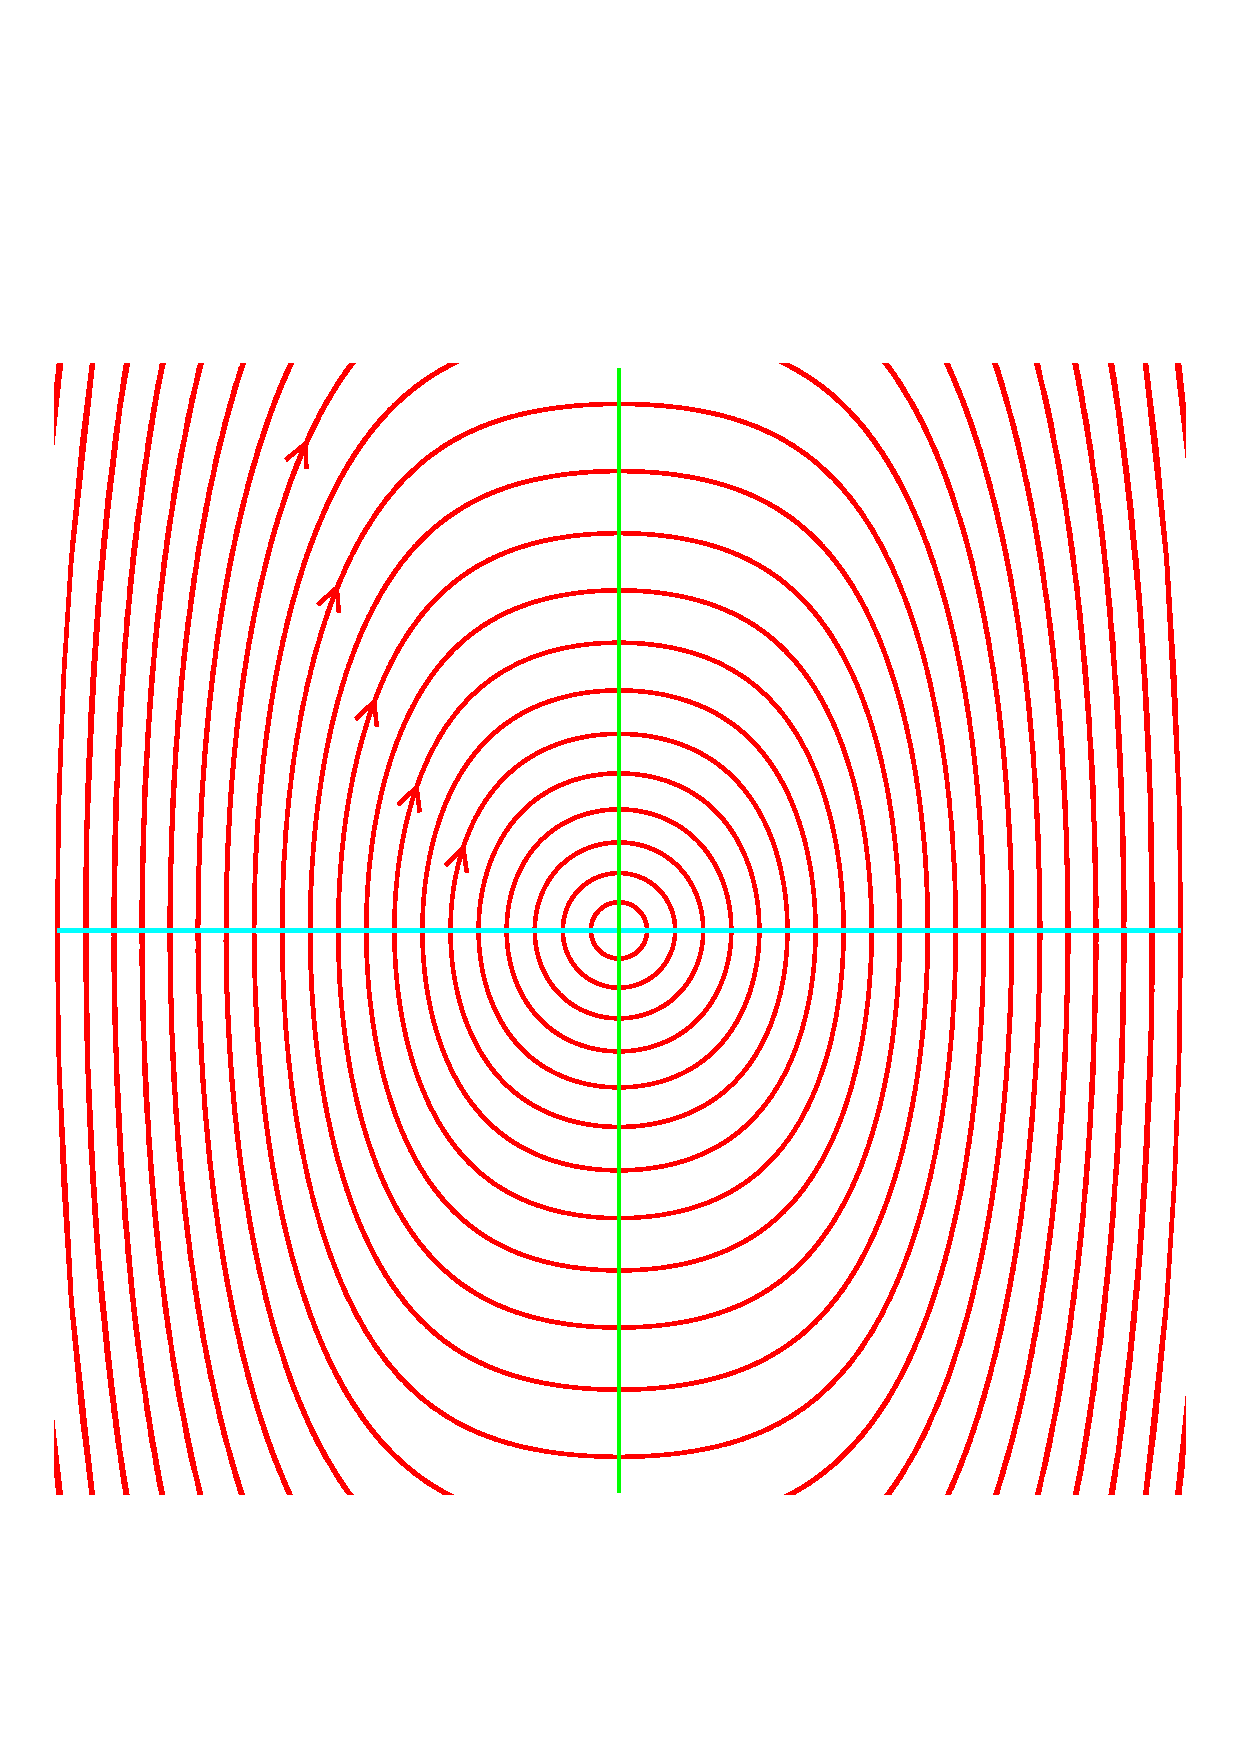
\includegraphics[scale=0.15]{images/hard_spring.pdf} &
     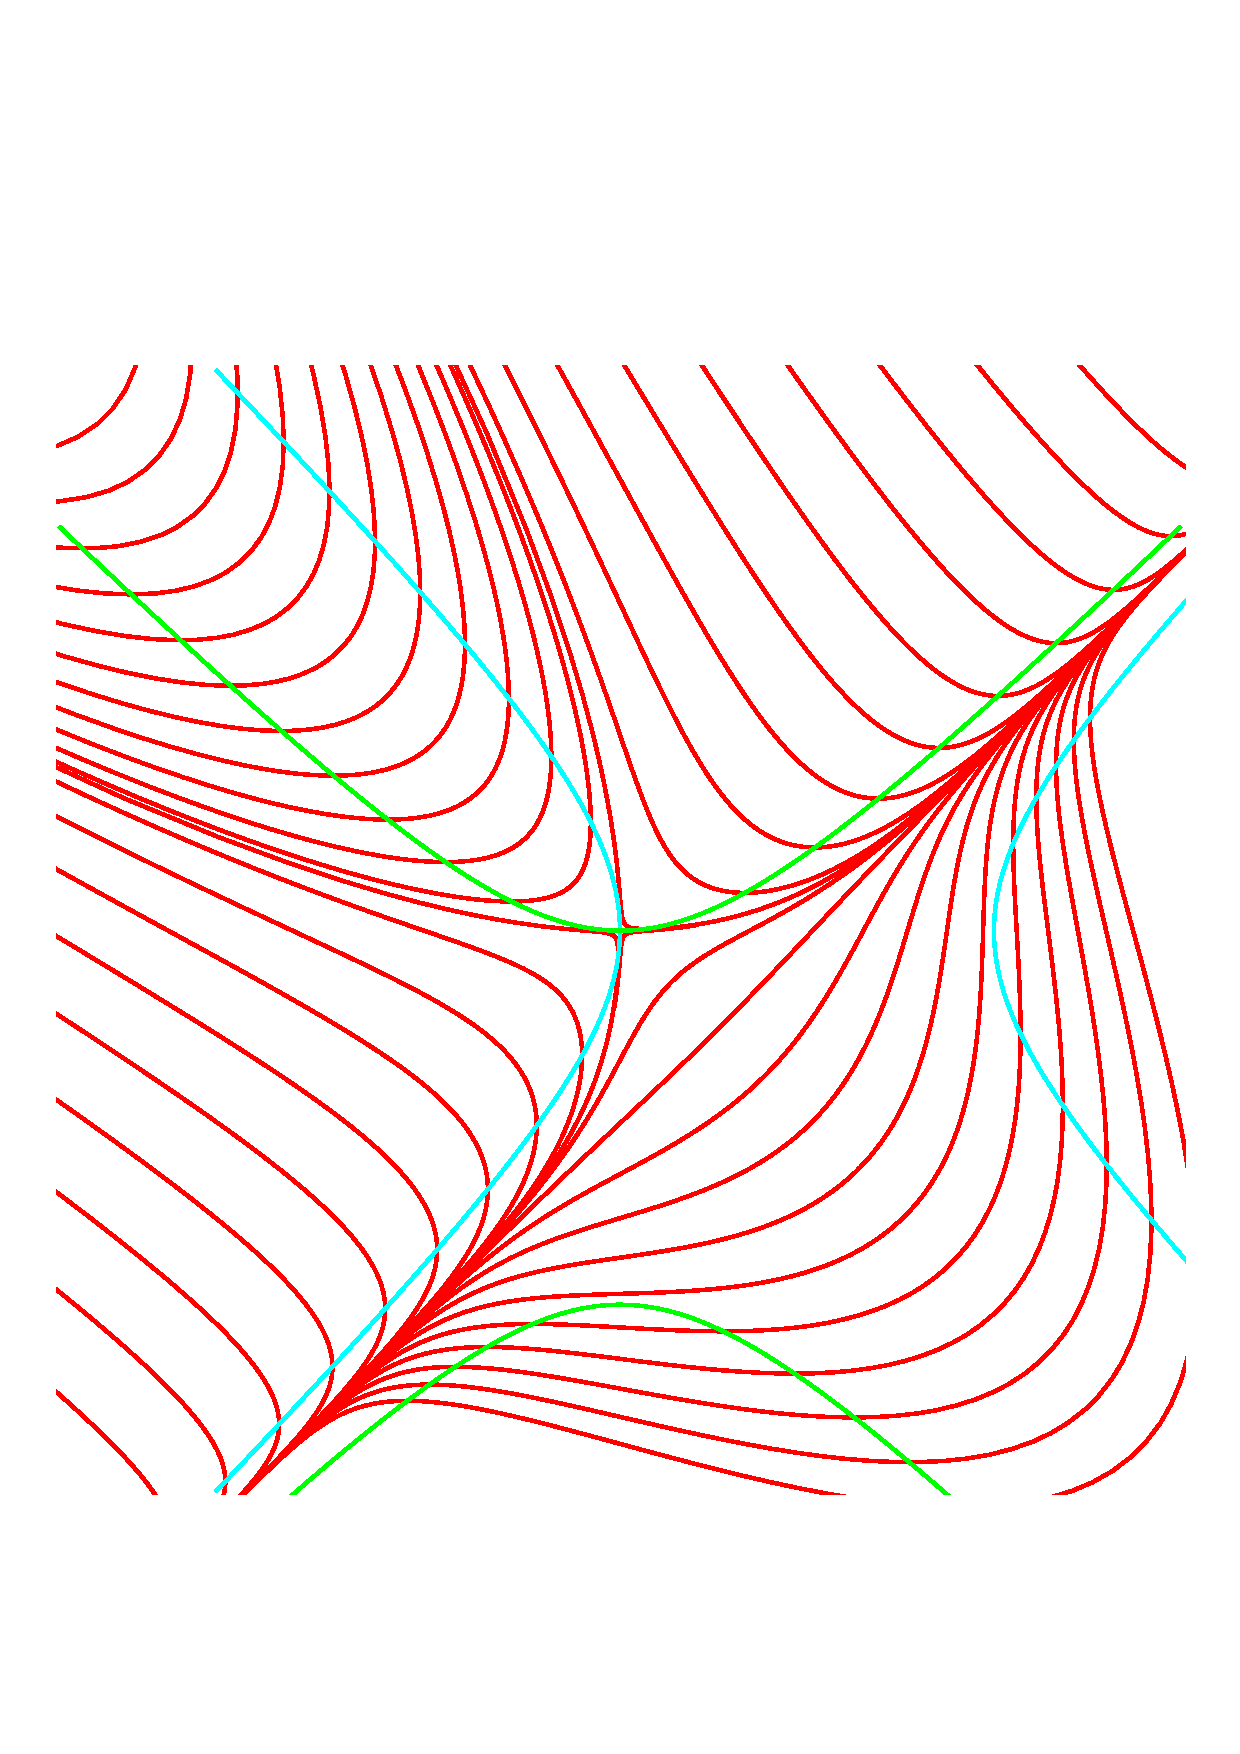
\includegraphics[scale=0.15]{images/limit_line.pdf} \\
     A & B \\
     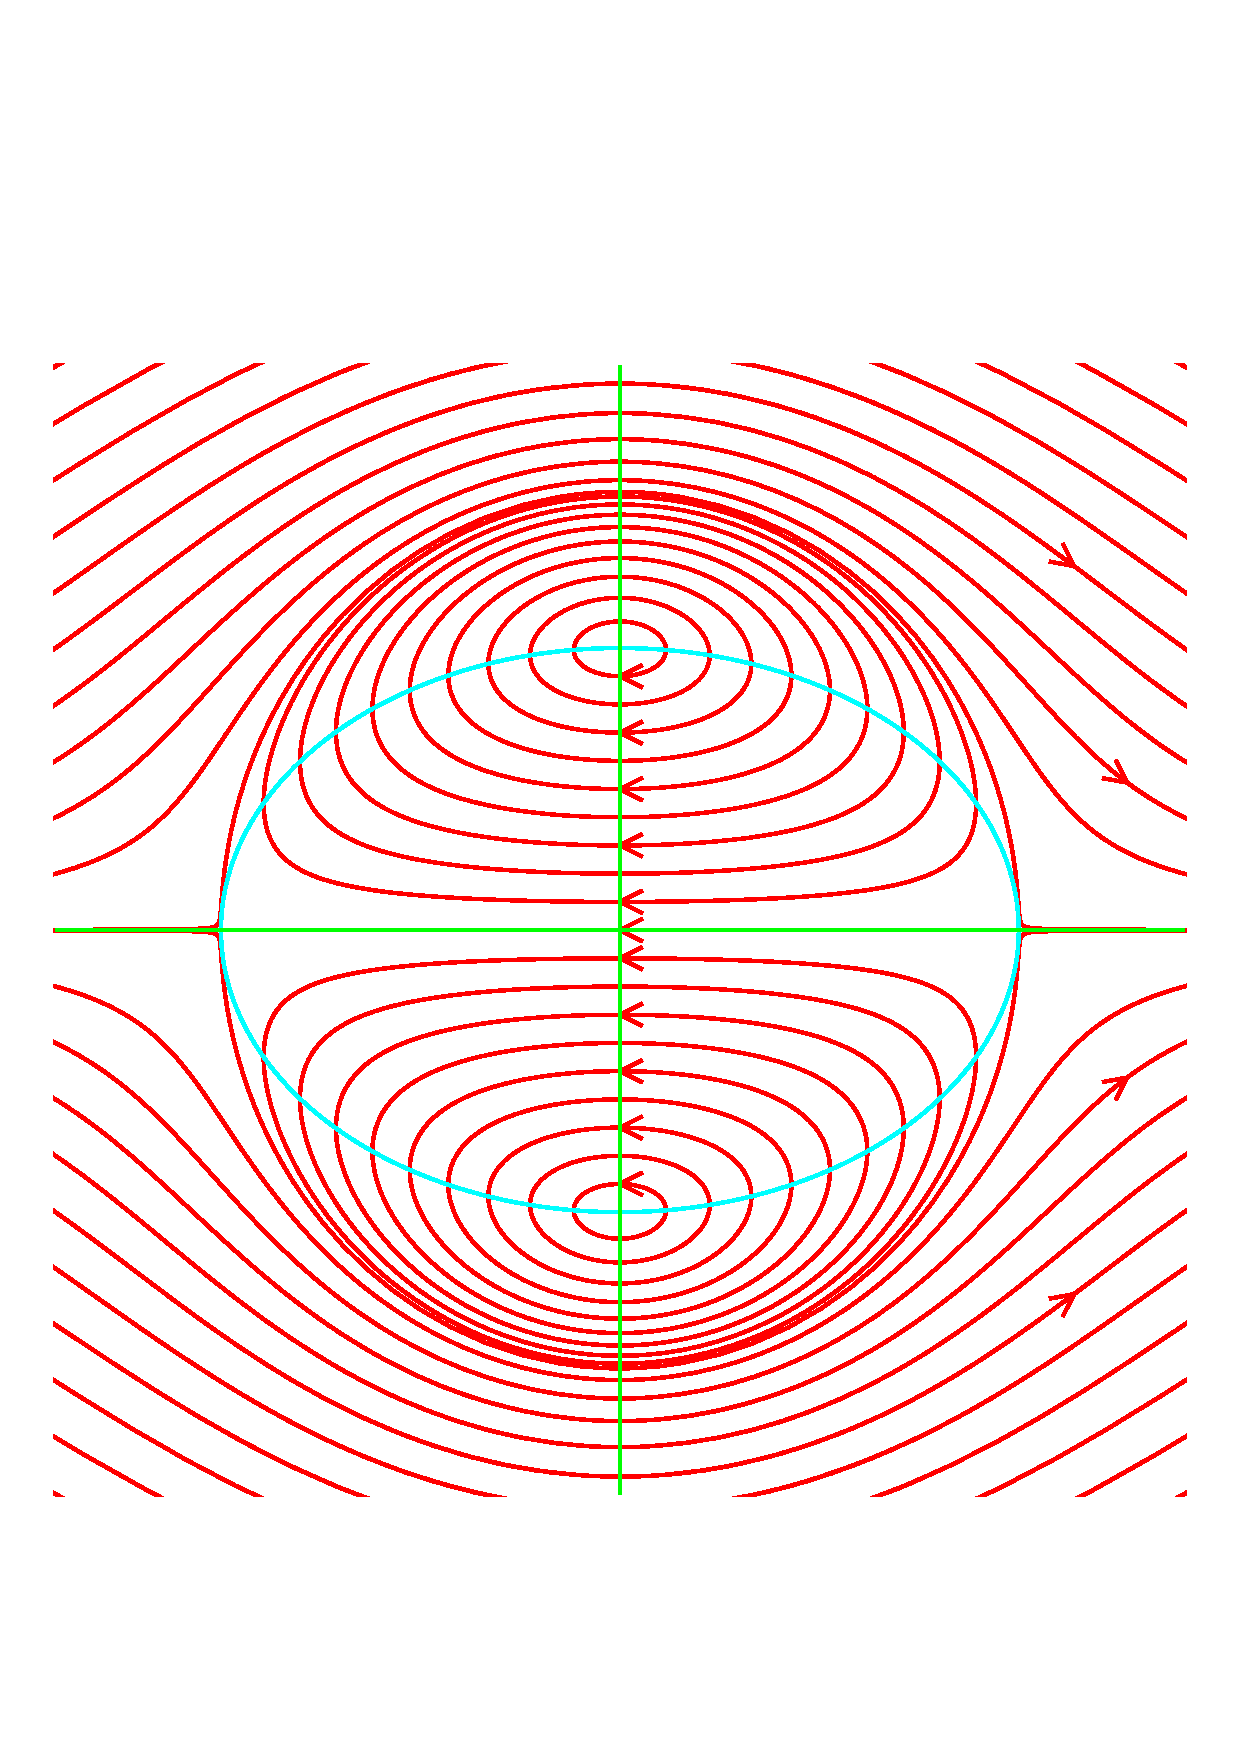
\includegraphics[scale=0.15]{images/misc_e.pdf} &
     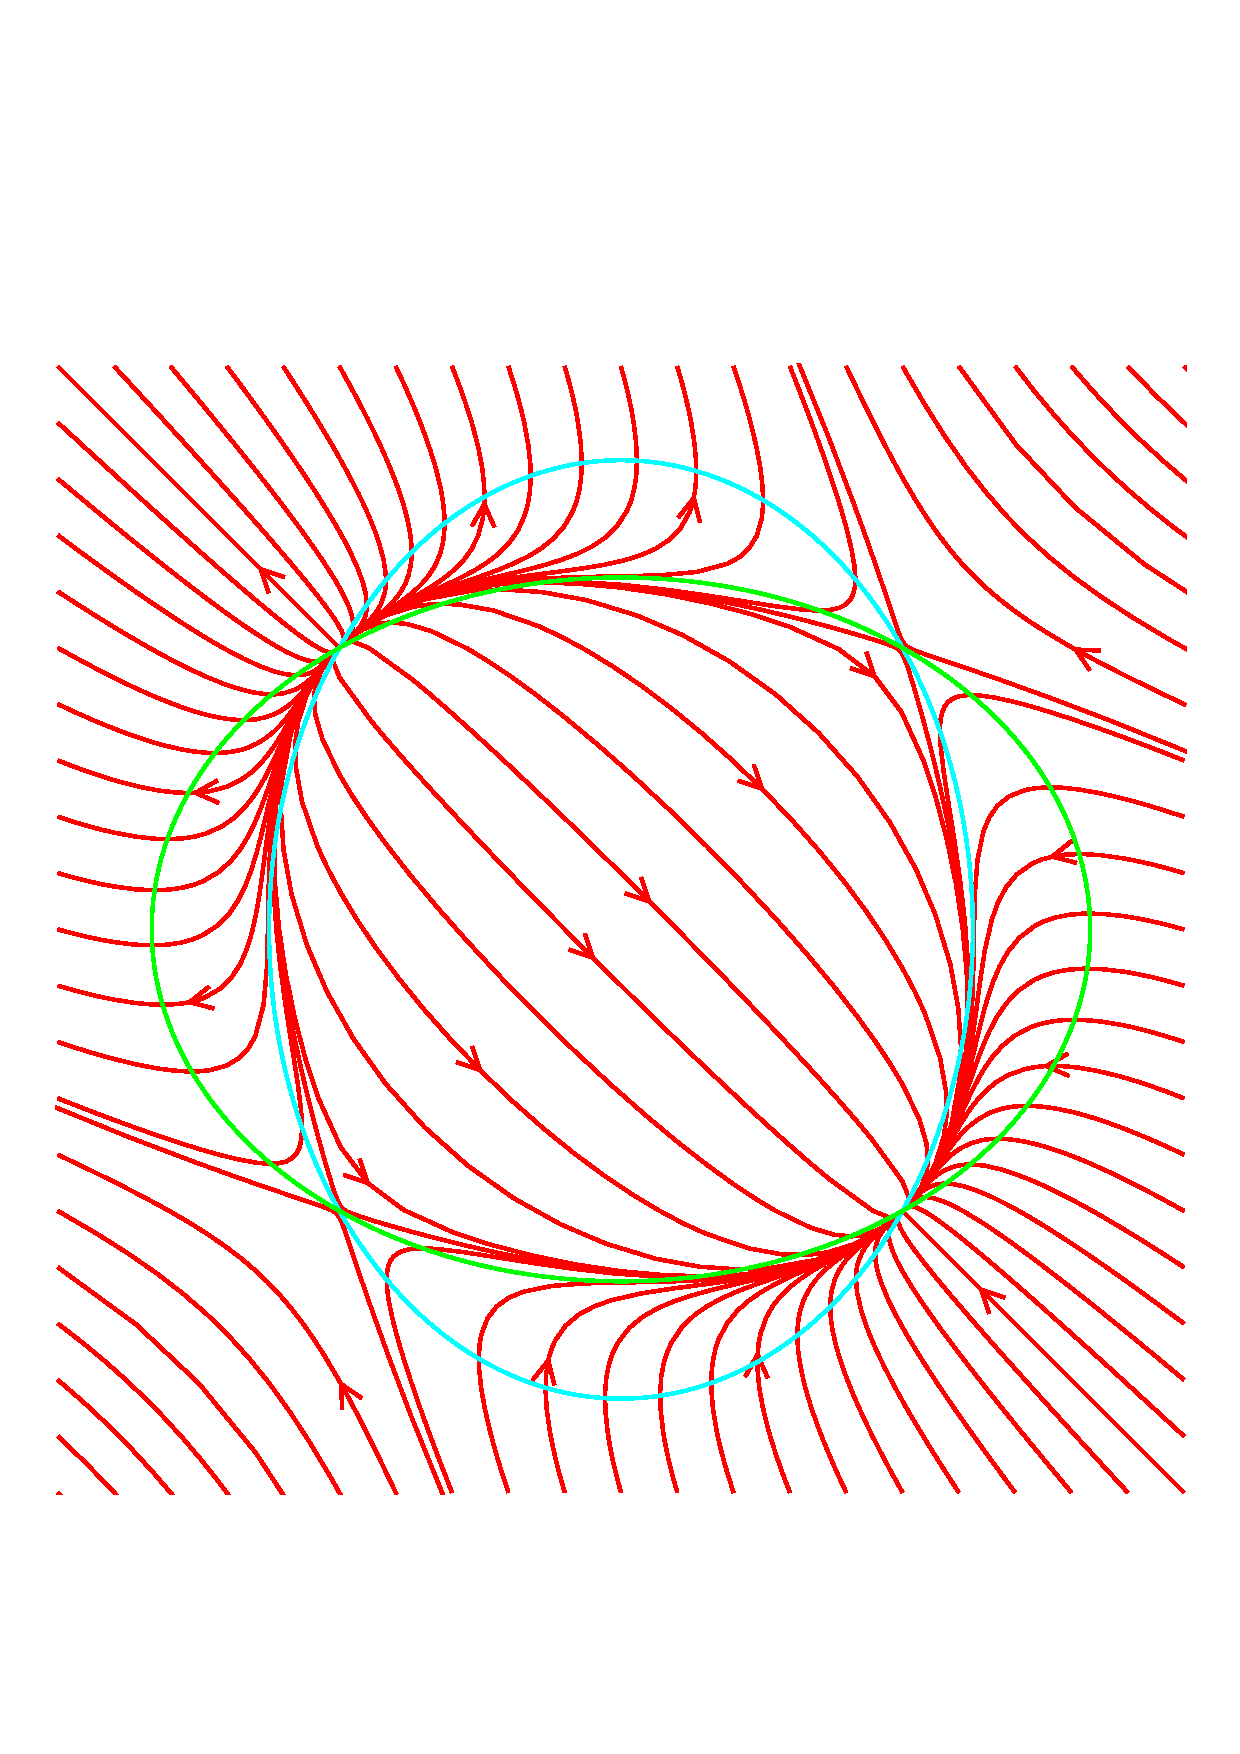
\includegraphics[scale=0.15]{images/quad_a.pdf} \\
     C & D \\
   \end{array}
 \]}%
 \only<2>{\[ \text{A} : 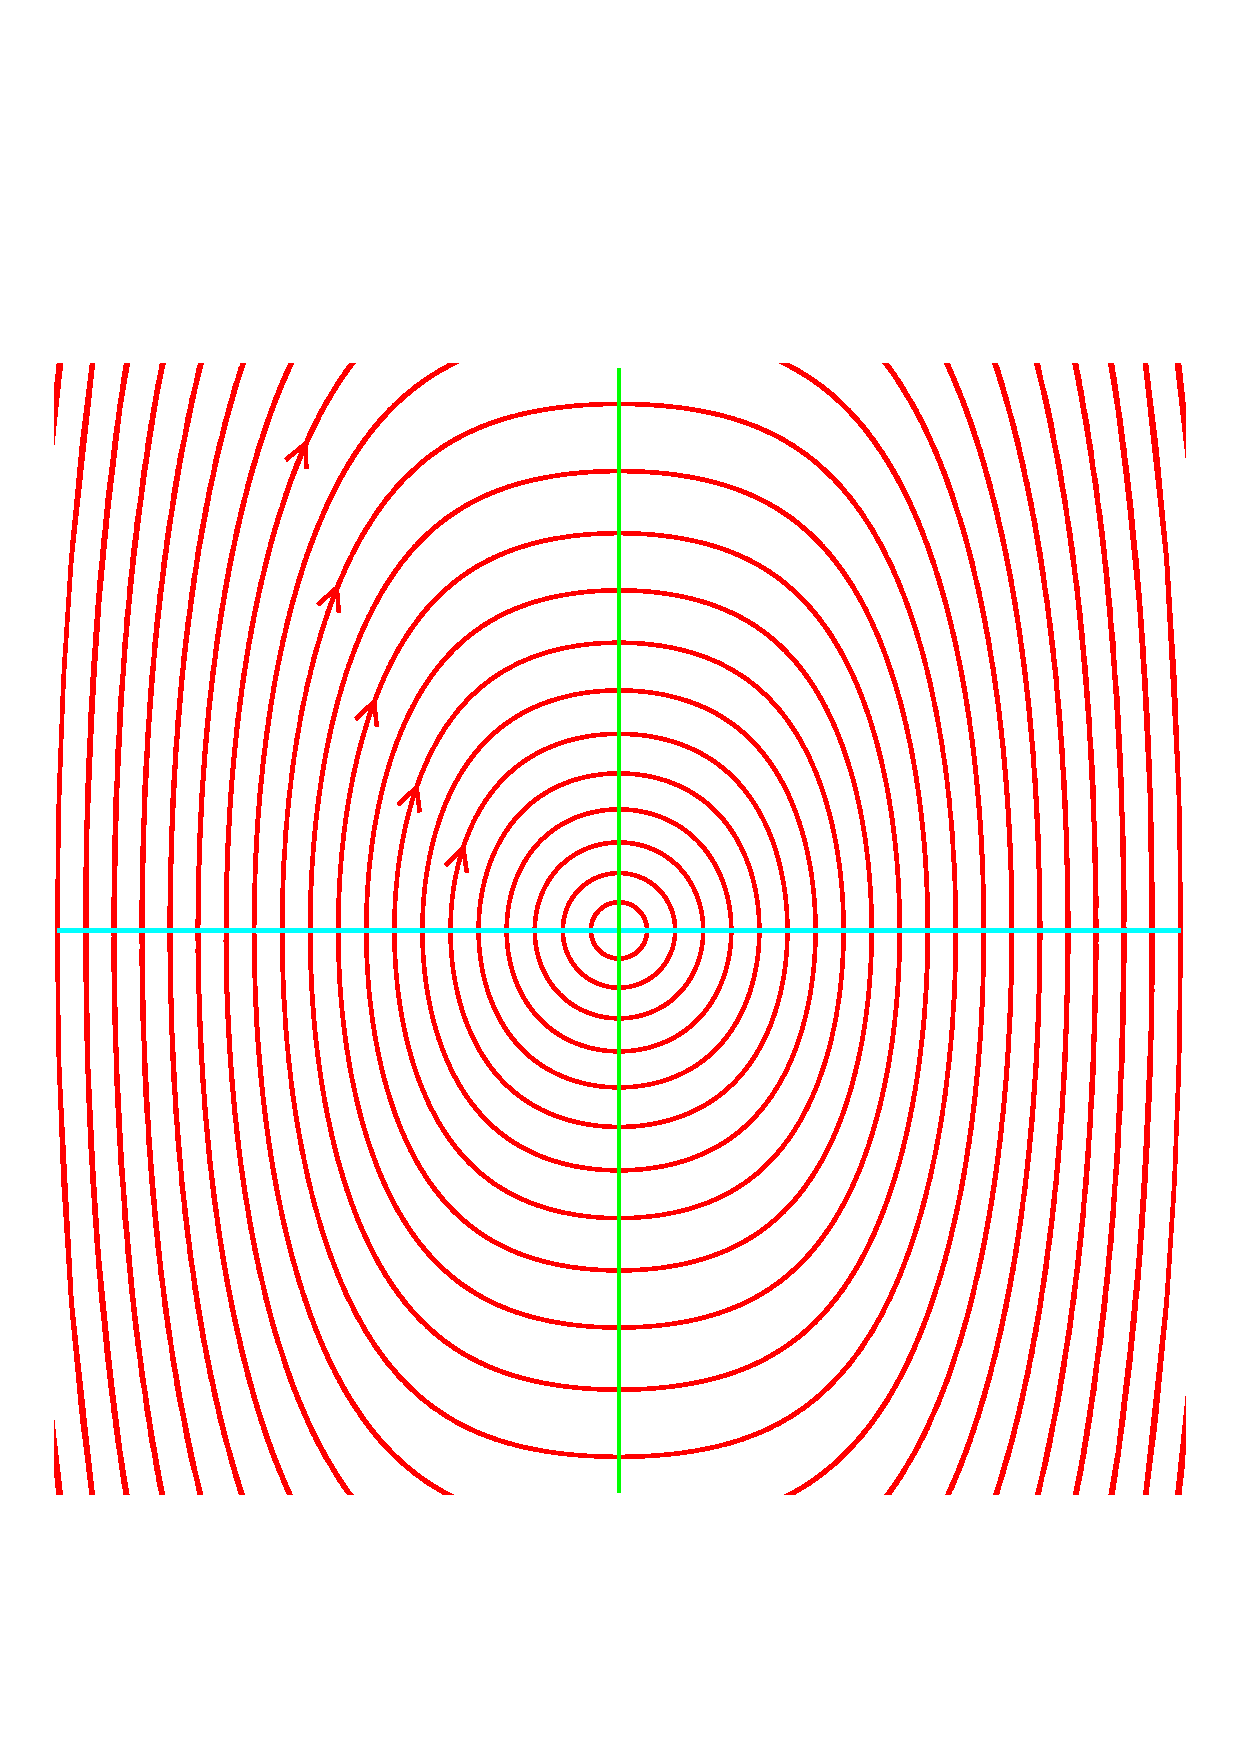
\includegraphics[scale=0.3]{images/hard_spring.pdf} \]}%
 \only<3>{\[ \text{B} : 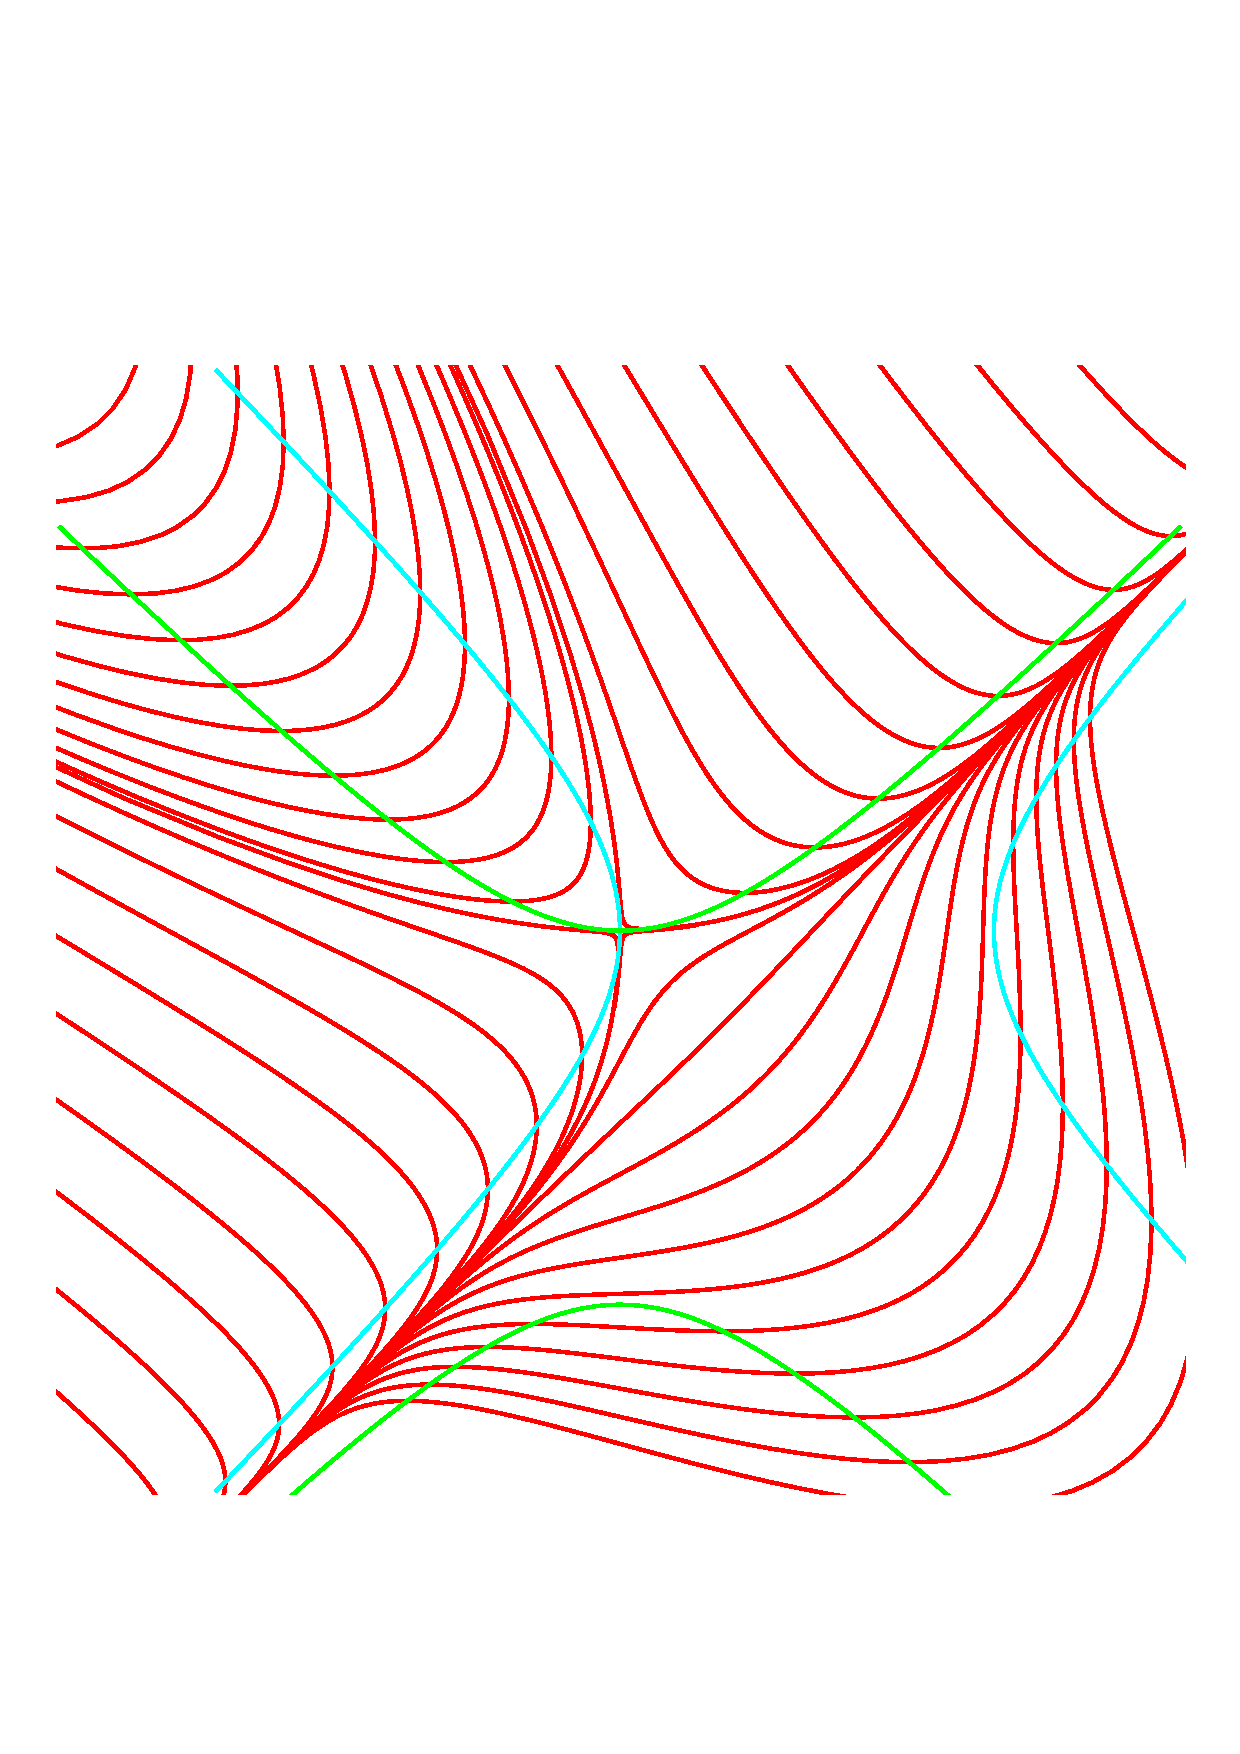
\includegraphics[scale=0.3]{images/limit_line.pdf} \]}%
 \only<4>{\[ \text{C} : 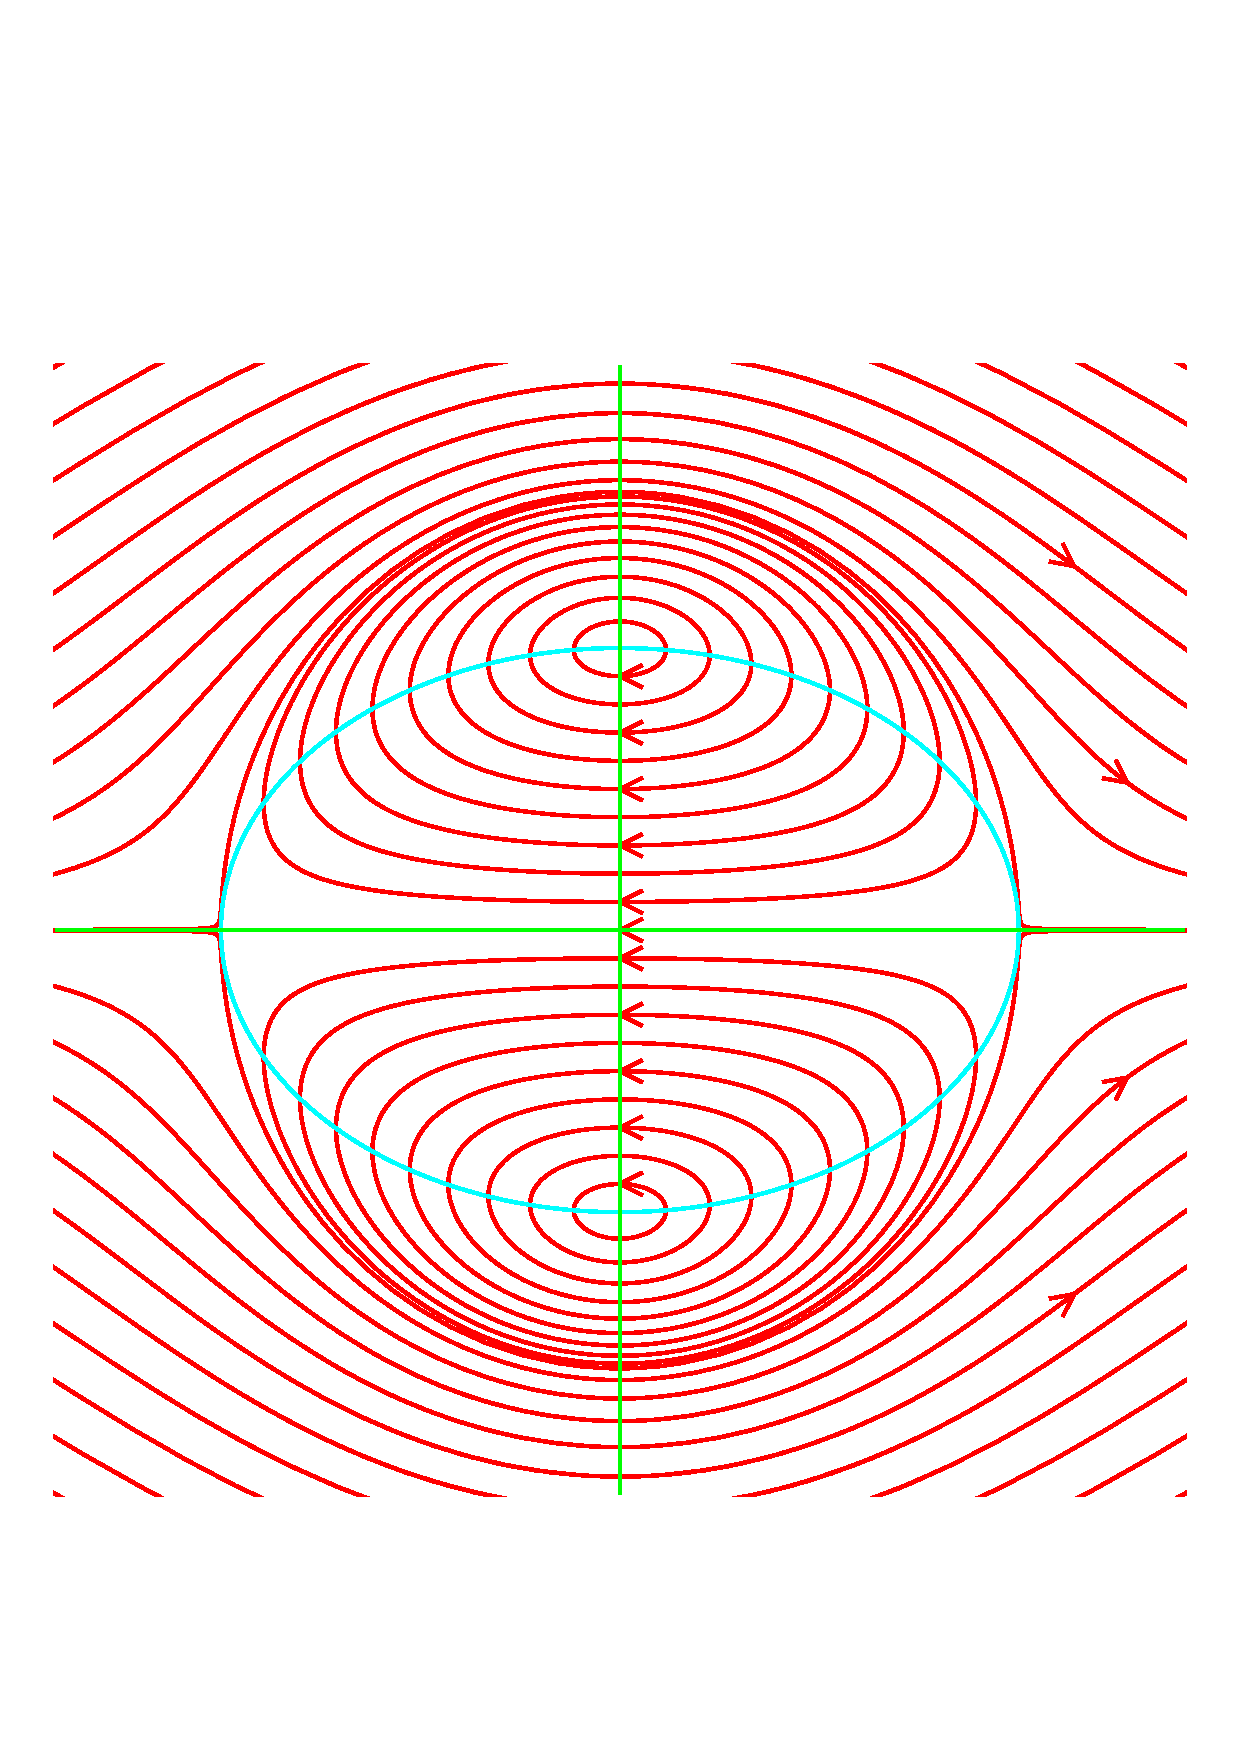
\includegraphics[scale=0.3]{images/misc_e.pdf} \]}%
 \only<5>{\[ \text{D} : 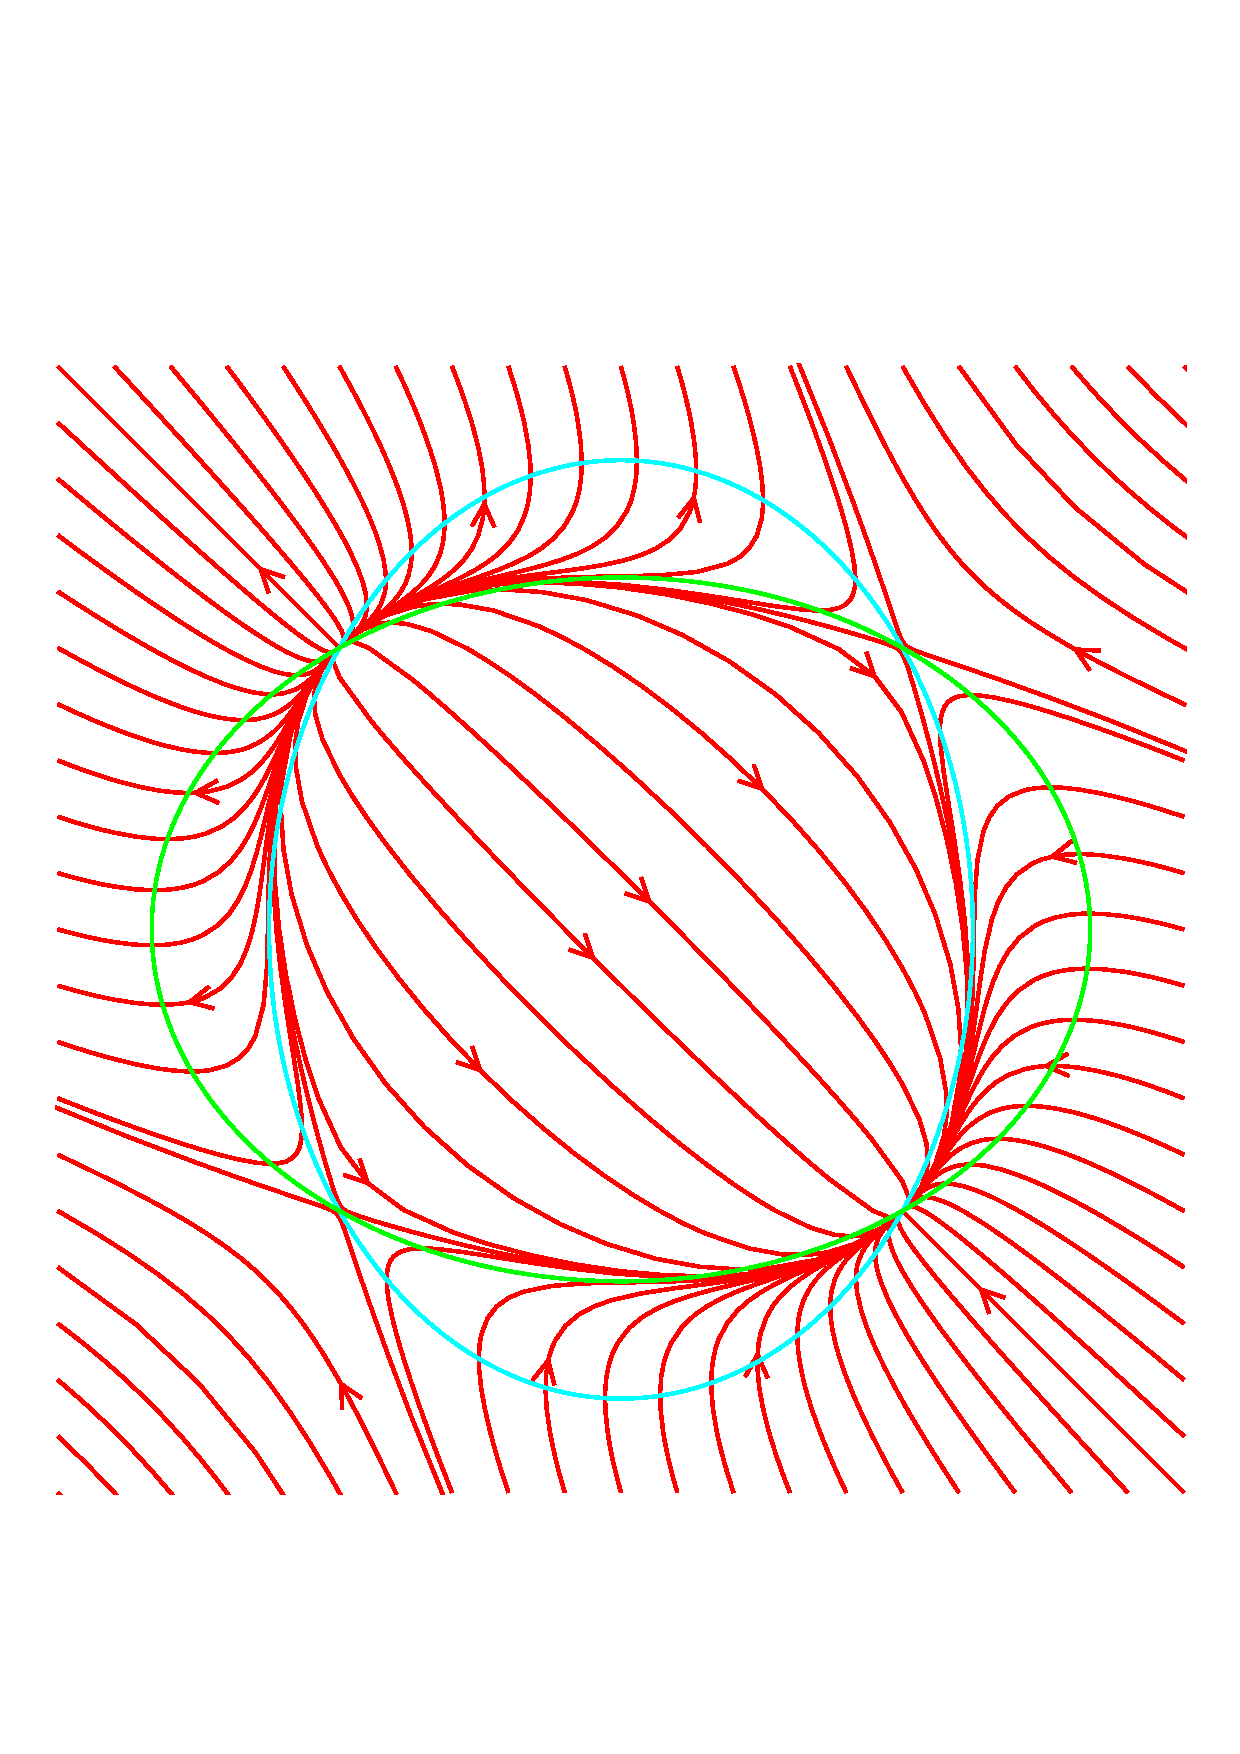
\includegraphics[scale=0.3]{images/quad_a.pdf} \]}%
 \only<6>{\[ \begin{array}{cc}
     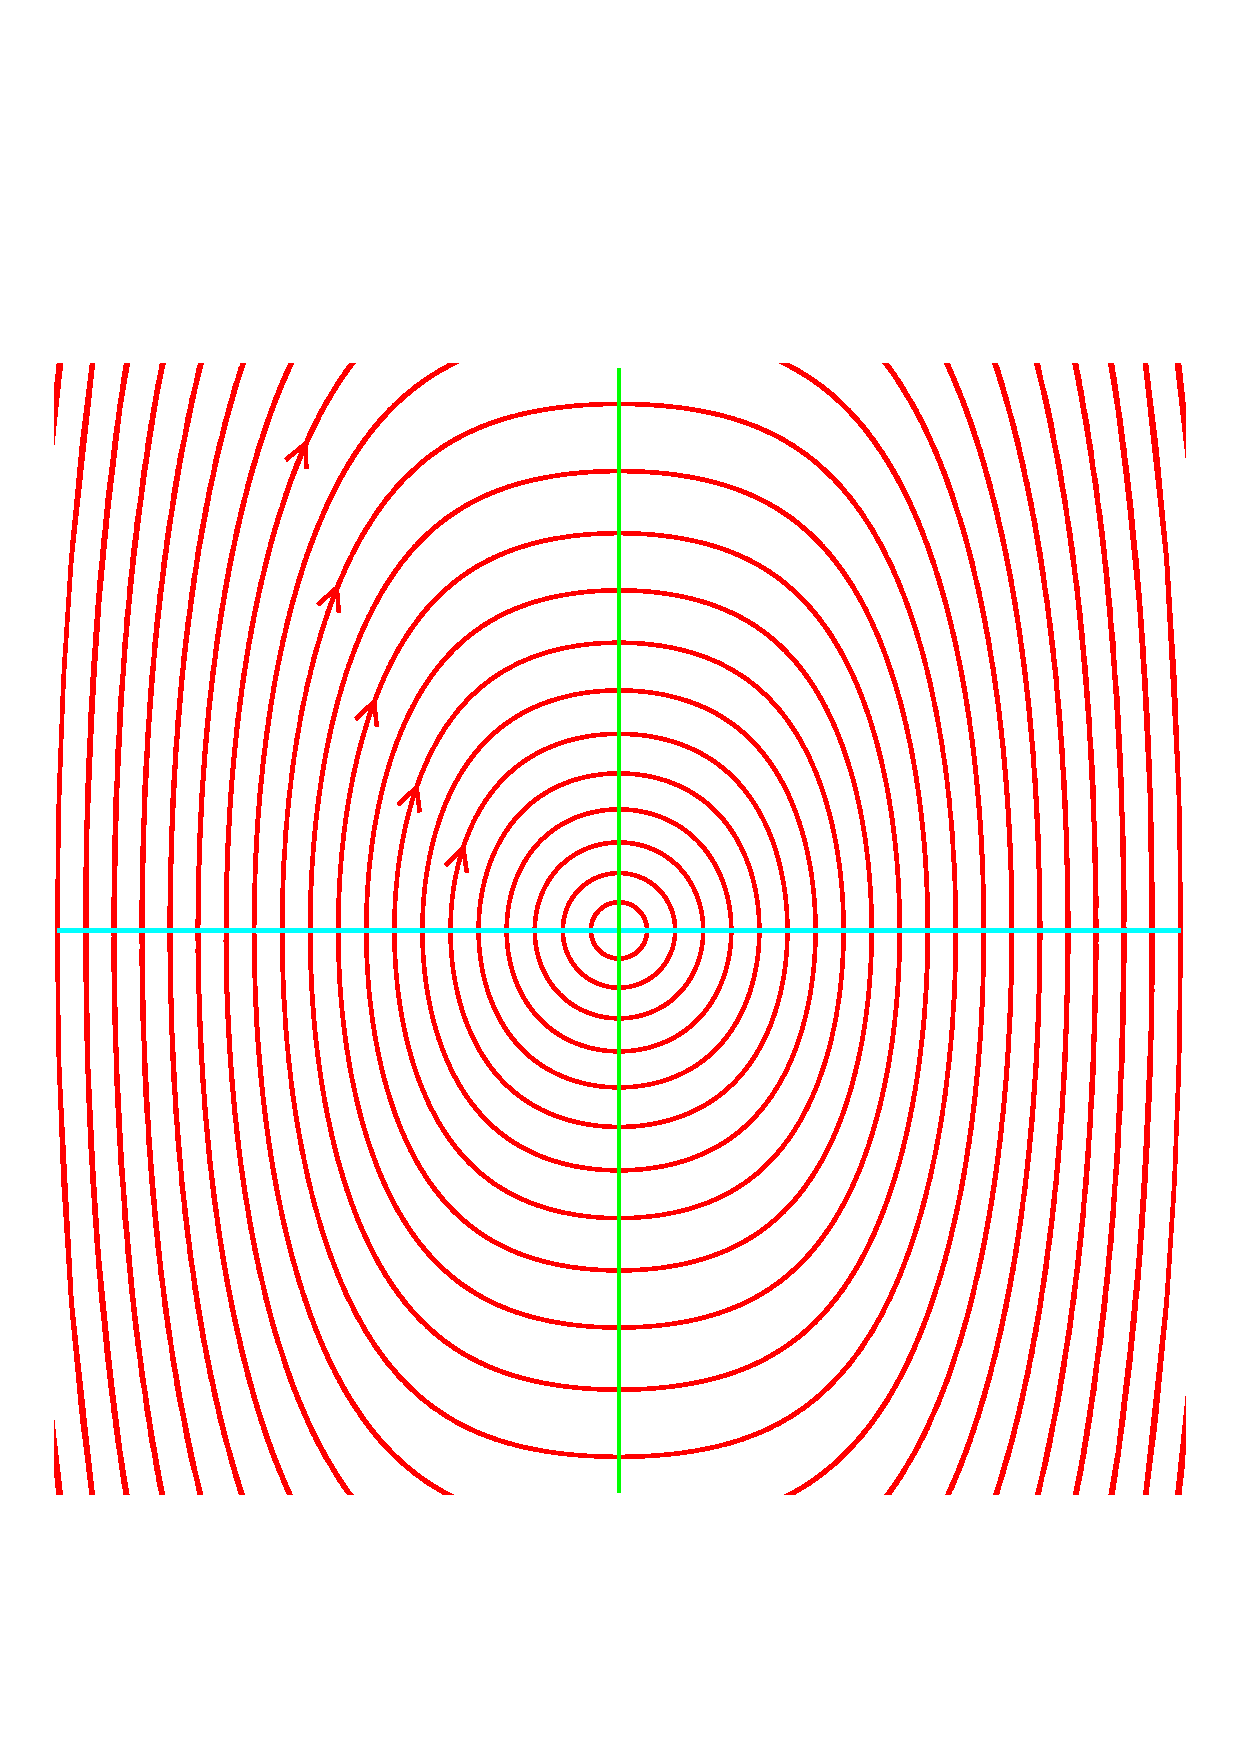
\includegraphics[scale=0.15]{images/hard_spring.pdf} &
     \includegraphics[scale=0.15]{images/limit_line.pdf} \\
     A & B \\
     \includegraphics[scale=0.15]{images/misc_e.pdf} &
     \includegraphics[scale=0.15]{images/quad_a.pdf} \\
     C & D \\
   \end{array}
 \]}%
 \vfill
 \only<1-5>{Which picture shows $\dot{x}=x^2+2y^2-\half$, $\dot{y}=-\sqrt{2}xy$?}
 \only<6>{Picture C shows $\dot{x}=x^2+2y^2-\half$, $\dot{y}=-\sqrt{2}xy$.}
\end{frame}

\begin{frame}[t]
 \frametitle{Linear systems}
 A \emph{(first order, autonomous) linear system} has the form
 \[ \dot{x} = \frac{dx}{dt} = ax + by \hspace{4em}
    \dot{y} = \frac{dy}{dt} = cx + dy \hspace{4em} 
    \bbm \dot{x}\\\dot{y}\ebm =
     \frac{d}{dt}\bbm x\\ y\ebm =
     \bbm a&b \\ c&d\ebm \bbm x\\ y\ebm
 \]
 \uc<2->{Linear systems are the easiest kind of planar differential equations.}\\
 \uc<3->{They will also help us to understand nonlinear systems.}

 \medskip

 \uc<4->{\begin{example*}{\!\!}\vspace{-2ex}
  \[ \begin{array}{llll}
    \text{Suppose $b=c=0$, so} &
    \begin{array}{rl}\dot{x}&=ax \\ \dot{y} &=dy \end{array} &
    \text{ or } &
    \bbm\dot{x}\\ \dot{y}\ebm=\bbm a&0 \\ 0&d\ebm\bbm x\\ y\ebm \\ \\
    \uc<5->{\text{The solution is}} &
    \uc<5->{\begin{array}{rl}
     x &= e^{at}x_0 \\
     y &= e^{dt}y_0
    \end{array}} &
    \uc<6->{\text{ or }} &
    \uc<6->{\bbm x\\ y\ebm=
     \bbm e^{at}&0 \\ 0&e^{dt}\ebm\bbm x_0\\ y_0\ebm.}
  \end{array} \]
 \end{example*}}

 \uc<7->{\begin{example*}{\!\!}\vspace{-2ex}
  \[ \begin{array}{llll}
    \text{Suppose } &
    \begin{array}{rl}\dot{x}&=y \\ \dot{y} &=-x \end{array} &
    \text{ or } &
    \bbm\dot{x}\\ \dot{y}\ebm=\bbm 0&1 \\ -1&0\ebm\bbm x\\ y\ebm \\ \\
    \uc<8->{\text{Solution:}} &
    \uc<8->{\begin{array}{rl}
     x &= x_0\cos(t)+y_0\sin(t) \\
     y &= y_0\cos(t)-x_0\sin(t)
    \end{array}} &
    \uc<9->{\text{ or }} &
    \uc<9->{\bbm x\\ y\ebm=
     \bbm \cos(t)&\sin(t) \\ -\sin(t)&\cos(t)\ebm\bbm x_0\\ y_0\ebm.}
  \end{array} \]
 \end{example*}}
\end{frame}

\begin{frame}[t]
 \frametitle{Reminder of simple harmonic motion}
 
 \begin{proposition*}{}
  Suppose that $x$ is a function of $t$ such that $\ddot{x}=-\om^2 x$;
  then $x(t)=A\cos(\om t)+B\sin(\om t)$ for some constants $A$ and $B$.
 \end{proposition*}
 \uc<2->{\begin{proof}
  Put $A=x(0)$ and $B=\dot{x}(0)/\om$\uc<3->{ and
  $u(t)=A\cos(\om t)+B\sin(\om t)$}\uc<4->{ and $v(t)=x(t)-u(t)$.}\uc<5->{  We want to
  show that $x(t)=u(t)$, so we must show that $v(t)=0$.}\uc<6->{  Note that 
  \begin{align*}
   \dot{u}(t) &= -A\om\sin(\om t) + B\om\cos(\om t) \\
   \uc<7->{\ddot{u}(t)} &\uc<7->{= -A\om^2\cos(\om t) - B\om^2\sin(\om t)} 
                \uc<8->{= -\om^2 u(t)} \\
   \uc<9->{\ddot{v}(t)} &\uc<9->{= \ddot{x}(t) - \ddot{u}(t)} 
                \uc<10->{= -\om^2 x(t) + \om^2 u(t)} 
                \uc<11->{= -\om^2 v(t)} \\
   \uc<12->{v(0)} &\uc<12->{= x(0) - A = 0} \\
   \uc<13->{\dot{v}(0)} &\uc<13->{= \dot{x}(0) - B\om = 0.}  
  \end{align*}}
  \uc<14->{Now put $E(t)=\om^2 v(t)^2+\dot{v}(t)^2$}\uc<15->{, so
  $E(0)=\om^2 v(0)^2+\dot{v}(0)^2=0$.}\uc<16->{  Also:
  \[ \dot{E}(t) = 2\om^2 v(t)\dot{v}(t) + 2 \dot{v}(t)\ddot{v}(t)
      \uc<17->{= 2\dot{v}(t) (\om^2 v(t) + \ddot{v}(t))}\uc<18->{ = 0.}
  \]}
  \uc<19->{This means that $E$ is constant}\uc<20->{, and $E(0)=0$, so $E(t)=0$ for all
  $t$.}\uc<21->{  As squares are always nonnegative, the only way that $E(t)$
  can be zero is if $v(t)=0$ and $\dot{v}(t)=0$.}\uc<22->{  We thus have $v=0$
  as required.}
 \end{proof}}
\end{frame}

\begin{frame}<handout:0>[t]
 \frametitle{Question}
 A \emph{(first order, autonomous) linear system} has the form
 \[ \dot{x} = \frac{dx}{dt} = ax + by \hspace{4em}
    \dot{y} = \frac{dy}{dt} = cx + dy \hspace{4em} 
    \bbm \dot{x}\\\dot{y}\ebm =
     \frac{d}{dt}\bbm x\\ y\ebm =
     \bbm a&b \\ c&d\ebm \bbm x\\ y\ebm
 \]

 \reminderbar
 
 Which of the following is a first order, autonomous linear system?
 \begin{itemize}
  \item[(a)] $\dot{x}=3x+t$, $\dot{y}=4y-t$
  \item[(b)] $\dot{x}=3x-y$, $\dot{y}=x+9y$
  \item[(c)] $\dot{x}=2x-1$, $\dot{y}=2+5y$
  \item[(d)] $\ddot{x}=y$, $\ddot{y}=x$.
 \end{itemize}

 \uc<2->{
 Only~(b) is a first order, autonomous linear system.}
 \begin{itemize}
  \item<3->[(a)] is of first order but not autonomous or linear
  \item<4->[(c)] is of first order and autonomous but not linear
  \item<5->[(d)] is of second order, autonomous and linear.
 \end{itemize}
\end{frame}

\begin{frame}<handout:0>[t]
 \frametitle{Question}

 What is the solution to $\dot{x}=y$ and $\dot{y}=-x$ with 
 $x=0$ and $y=5$ when $t=0$?

 \bigskip\pause

 The general solution is 
 \[ x = x_0\cos(t)+y_0\sin(t) \hspace{5em}
    y = y_0\cos(t)-x_0\sin(t).
 \]
 \pause
 Here $x_0=0$ and $y_0=5$, so we just get
 \[ x = 5\sin(t) \hspace{5em}
    y = 5\cos(t).
 \]
\end{frame}

\begin{frame}[t]
 \frametitle{Linear systems}
 A \emph{(first order, autonomous) linear system} has the form
 \[ \dot{x} = \frac{dx}{dt} = ax + by \hspace{4em}
    \dot{y} = \frac{dy}{dt} = cx + dy \hspace{4em} \pause
    \bbm \dot{x}\\\dot{y}\ebm =
     \frac{d}{dt}\bbm x\\ y\ebm =
     \bbm a&b \\ c&d\ebm \bbm x\\ y\ebm
 \] \pause
 \vspace{-2ex}
 \reminderbar

 We put $u=\bbm x\\ y\ebm$ and $A=\bbm a&b\\ c&d\ebm$ so $\dot{u}=Au$.\pause
 To solve the system, we first need to find eigenvalues \bhan{特征值} and
 eigenvectors \bhan{特征向量} of $A$. \pause Put 
 \[ \RED{\tau} = \text{trace}(A) = \RED{a+d} \;\text{\bhan{迹}} \hspace{4em}
    \OLG{\dl} = \det(A) = \OLG{ad-bc} \;\text{\bhan{行列式}}
 \]
 \pause
 \vspace{-5ex}
 \begin{align*}
  \chi_A(t) &= \text{ characteristic polynomial }
     = \det(A-tI)
     = \det\bbm a-t & b \\ c & d-t \ebm \\
     &= (a-t)(d-t) - bc 
     = t^2 - (\RED{a+d})t + (\OLG{ad-bc})
     = t^2-\RED{\tau} t + \OLG{\dl}.
 \end{align*}
 \pause 
 The eigenvalues are the roots of $\chi_A(t)$, which are
 \[ \lm_1 = \half(\tau-\sqrt{\tau^2-4\dl}) \hspace{5em}
    \lm_2 = \half(\tau+\sqrt{\tau^2-4\dl}).
 \]\pause
 These might be real numbers \bhan{实数} or complex numbers \bhan{复数}.\\
 \pause
 \[ \RED{\lm_1+\lm_2}=\RED{\tau} \hspace{4em} \OLG{\lm_1\lm_2}=\OLG{\dl} \]
\end{frame}

\begin{frame}<handout:0>[t]
 \frametitle{Question}
 \[ \bbm \dot{x}\\ \dot{y}\ebm=\bbm a&b\\ c&d\ebm\bbm x\\ y\ebm
    \hspace{3em}
    \begin{array}{rl}
     \tau &= a+b \\ \dl &= ad-bc
    \end{array}
    \hspace{3em}
    \begin{array}{rl}
     \lm_1 &= \half(\tau - \sqrt{\tau^2-4\dl}) \\
     \lm_2 &= \half(\tau + \sqrt{\tau^2-4\dl}).
    \end{array}
 \]

 \reminderbar
 Which of the following has real eigenvalues?
 \begin{itemize}
  \item[(a)] $A=\bbm 0 & 1\\-2 & 0\ebm$\uc<3->{; $\tau=0,\;\dl=2$\;}\uc<4->{; $\tau^2-4\dl=-8<0$}
  \item[(b)] $A=\bbm 1 &-1\\ 1 & 1\ebm$\uc<3->{; $\tau=2,\;\dl=2$\;}\uc<4->{; $\tau^2-4\dl=-4<0$}
  \item[(c)] $A=\bbm 7 &-2\\ 7 & 0\ebm$\uc<3->{; $\tau=7,\;\dl=14$}\uc<4->{; $\tau^2-4\dl=-7<0$}
  \item[(d)] $A=\bbm 3 & 3\\ 3 & 3\ebm$\;\;\;\uc<3->{; $\tau=6,\;\dl=0$\;}\uc<4->{; $\tau^2-4\dl=36>0$}.
 \end{itemize}
 \uc<2->{Eigenvalues are real if $\tau^2-4\dl\geq 0$.}\uc<5->{ Only~(d) has real eigenvalues. }
\end{frame}


\begin{frame}[t]
 \frametitle{Linear systems with real eigenvalues}
 \[ \bbm \dot{x}\\ \dot{y}\ebm=\bbm a&b\\ c&d\ebm\bbm x\\ y\ebm
    \hspace{3em}
    \begin{array}{rl}
     \tau &= a+b \\ \dl &= ad-bc
    \end{array}
    \hspace{3em}
    \begin{array}{rl}
     \lm_1 &= \half(\tau - \sqrt{\tau^2-4\dl}) \\
     \lm_2 &= \half(\tau + \sqrt{\tau^2-4\dl}).
    \end{array}
 \]

 \reminderbar

 Suppose for the moment that $\tau^2>4\dl$, so $\lm_1$ and $\lm_2$ are
 real, and $\lm_1<\lm_2$.  \\ \pause
 We can find eigenvectors $v_1$ and $v_2$
 such that $Av_1=\lm_1v_1$ and $Av_2=\lm_2v_2$.  \pause

 \medskip

 Now suppose that $u=c_1e^{\lm_1t}v_1+c_2e^{\lm_2t}v_2$ for some
 constants $c_1$ and $c_2$.  \pause Then 
 \[ \dot{u} =
    c_1\lm_1e^{\lm_1t}v_1 + c_2\lm_2e^{\lm_2t}v_2 \pause = 
    c_1e^{\lm_1t}Av_1 + c_2e^{\lm_2t}Av_2 \pause = Au,
 \] \pause
 so we have a solution to our system of equations.

 \pause \medskip

 If $\lm_1,\lm_2<0$ then $u\to 0$ as $t\to\infty$. \\\pause

 \medskip

 If $\lm_1<0<\lm_2$ then when $t$ is large we can ignore
 $c_1e^{\lm_1t}v_1$ and $u\simeq c_2e^{\lm_2t}v_2$.\\  \pause 

 \medskip

 If $0<\lm_1<\lm_2$ then both terms will be very large when $t$ is
 large, but the term $c_2e^{\lm_2t}v_2$ will still grow much more
 quickly than $c_1e^{\lm_1t}v_1$.
\end{frame}

\begin{frame}[t]
 \frametitle{Linear systems with real eigenvalues --- example}
 
 Consider the system
 \[ \begin{array}{rl}
     \dot{x} &= 2y \\ \dot{y} &= x + y
    \end{array}
    \hspace{4em}
    \bbm \dot{x} \\ \dot{y} \ebm = 
    A\bbm x \\ y \ebm, \text{ where }
    A = \bbm 0 & 2 \\ 1 & 1 \ebm
 \]\pause 
 \[ \tau = \text{trace}(A) = 0+1 = 1 \hspace{4em}
    \dl = \det(A) = 0\tm 1 - 2\tm 1 = -2
 \]\pause 
 Characteristic polynomial 
 $\chi_A(t)=\det\bbm -t & 2 \\ 1 & 1-t \ebm = 
  t^2 - t - 2 = t^2 - \tau t + \dl
 $.\\ \pause
 Roots $\lm_1,\lm_2$ are
 $\half(\tau\pm\sqrt{\tau^2-4\dl})=\half(1\pm\sqrt{9})=-1,2$
 (both real).\\ \pause

 \medskip

 Eigenvector $v_1=\bbm p\\ q\ebm$ should satisfy 
 $(A-\lm_1I)v_1=0$, or $(A+I)v_1=0$, or
 $\bbm 1&2\\1&2\ebm\bbm p\\ q\ebm=\bbm 0\\ 0\ebm$,
 or $p+2q=0$.  \pause Obvious choice is $v_1=\bbm -2\\ 1\ebm$.\\ \pause

 \medskip

 Eigenvector $v_2=\bbm p\\ q\ebm$ should satisfy 
 $(A-\lm_2I)v_2=0$, or $(A-2I)v_2=0$, or
 $\bbm -2&2\\1&-1\ebm\bbm p\\ q\ebm=\bbm 0\\ 0\ebm$,
 or $p-q=0$.  \pause Obvious choice is $v_2=\bbm 1\\ 1\ebm$.

\end{frame}

\begin{frame}[t]
 \frametitle{Linear systems with real eigenvalues --- example}

 \[ \bbm \dot{x}\\\dot{y}\ebm = \bbm 0&2\\ 1&1\ebm\bbm x\\ y\ebm
    \hspace{3em}
    \text{ eigenvectors } \bbm -2\\ 1\ebm,\bbm 1 \\ 1\ebm
    \text{ with eigenvalues } -1,2.
 \]

 \reminderbar

 Solutions have the form 
 \[ \bbm x \\ y \ebm = 
    c_1e^{\lm_1t}v_1 + c_2e^{\lm_2t}v_2 \pause =
    c_1e^{-t}\bbm -2\\ 1\ebm + c_2e^{2t}\bbm 1\\1\ebm \pause =
    \bbm -2c_1e^{-t} + c_2e^{2t} \\
         c_1e^{-t} + c_2e^{2t} \ebm.
 \]\pause 
 The values at time $t=0$ are 
 \[ \bbm x_0 \\ y_0 \ebm = 
    \bbm -2c_1e^{0} + c_2e^{0} \\
         c_1e^{0} + c_2e^{0} \ebm \pause =
    \bbm -2c_1 + c_2 \\ c_1 + c_2 \ebm \pause = 
    \bbm -2 & 1 \\ 1 & 1 \ebm \bbm c_1 \\ c_2 \ebm.
 \]\pause
 Often we do not know $c_1$ and $c_2$, but we do know $x_0$ and
 $y_0$.  \pause
 Then we can invert the above to find $c_1$ and $c_2$:
 \[ \bbm c_1 \\ c_2 \ebm = 
    \bbm -2 & 1 \\ 1 & 1 \ebm^{-1} \bbm x_0 \\ y_0 \ebm \pause = 
    \frac{1}{-3} \bbm 1 & -1 \\ -1 & -2 \ebm \bbm x_0 \\ y_0 \ebm
    \pause =
    \bbm y_0/3 - x_0/3 \\ 2y_0/3 + x_0/3 \ebm.
 \]
\end{frame}

\begin{frame}[t]
 \frametitle{Linear systems with real eigenvalues --- example}

 \[ \bbm x \\ y \ebm = 
    \bbm -2c_1e^{-t} + c_2e^{2t} \\
         c_1e^{-t} + c_2e^{2t} \ebm
    \hspace{4em}
    \bbm c_1 \\ c_2 \ebm = 
    \bbm y_0/3 - x_0/3 \\ 2y_0/3 + x_0/3 \ebm.
 \]

 \reminderbar

 For example, suppose we know that when $t=0$ we have $x=-1$ and
 $y=1$.  \pause
 Put $x_0=-1$ and $y_0=1$ in the right hand equation to get 
 $c_1=2/3$ and $c_2=1/3$. \pause
 Put these values in the left hand equation to get 
 \[ u = \bbm x \\ y \ebm = 
      \bbm -\frac{4}{3}e^{-t} + \frac{1}{3}e^{2t} \\
           \frac{2}{3}e^{-t} + \frac{1}{3}e^{2t} \ebm.
 \] \pause
 To check this, note that when $t=0$ it gives 
 $u=\bbm -4/3 + 1/3 \\ 2/3 + 1/3\ebm = \bbm -1 \\ 1\ebm = \bbm x_0\\y_0\ebm$
 as expected.\pause  Moreover:
 \begin{align*}
  \dot{u} &= \bbm  \frac{4}{3}e^{-t} + \frac{2}{3}e^{2t} \\
                  -\frac{2}{3}e^{-t} + \frac{2}{3}e^{2t} \ebm \\
  Au &= \bbm 0 & 2 \\ 1 & 1 \ebm 
        \bbm -\frac{4}{3}e^{-t} + \frac{1}{3}e^{2t} \\
              \frac{2}{3}e^{-t} + \frac{1}{3}e^{2t} \ebm 
      = \bbm  \frac{4}{3}e^{-t} + \frac{2}{3}e^{2t} \\
             -\frac{2}{3}e^{-t} + \frac{2}{3}e^{2t} \ebm, 
 \end{align*}
 so $\dot{u}=Au$ as expected.
\end{frame}


\begin{frame}<handout:0>[t]
 \frametitle{Question: what are the eigenvalues?}
 
 What are the eigenvalues of the matrix
 \[ A = \bbm 10 & 100 \\ 1000 & 10000 \ebm? \]
 \bigskip
 \uc<2->{The trace is $\tau=10+10000=10010$.\\}

 \uc<3->{The determinant is $\dl=10\tm 10000-100\tm 1000=0$.\\}

 \medskip

 \uc<4->{This means $\sqrt{\tau^2-4\dl}=\sqrt{\tau^2}=\tau$}\uc<5->{,
 so $\lm_1,\lm_2=(\tau\pm\tau)/2\uc<6->{=0,\tau}\uc<7->{=0,10010}$\uc<7->{.}}
\end{frame}

\begin{frame}[t]
 \frametitle{Linear systems with real eigenvalues --- reformulation}

 Consider again a system $\dot{u}=Au$, where $A$ has real eigenvalues
 $\lm_1<\lm_2$ and corresponding eigenvectors $v_1,v_2$.\\ \pause
 We can put $v_1$ and $v_2$ together to form a $2\tm 2$ matrix $V=\barmat{v_1}{v_2}$.\\
 \pause
 We also put 
 $ D = \bbm \lm_1 & 0 \\ 0 & \lm_2 \ebm $
 and 
 $ E = \bbm e^{\lm_1t} & 0 \\ 0 & e^{\lm_2t} \ebm$ 
 and $P=VEV^{-1}$.\\

 \bigskip\pause

 \begin{proposition*}{}
  We have $P=I$ when $t=0$, and $\dot{P}=AP$.  \\ \pause
  Also, the solution to $\dot{u}=Au$ with $u=u_0$ at $t=0$ is $u=Pu_0$.
 \end{proposition*}
\end{frame}

\begin{frame}[t]
 \frametitle{Linear systems with real eigenvalues --- reformulation}

 \[ V = \barmat{v_1}{v_2} \qquad
    D = \bbm \lm_1 & 0 \\ 0 & \lm_2 \ebm \qquad
    E = \bbm e^{\lm_1t} & 0 \\ 0 & e^{\lm_2t} \ebm \qquad
    P = VEV^{-1}
 \]

 Proposition: the solution to $\dot{u}=Au$ with $u=u_0$ at $t=0$ is $u=Pu_0$.

 \reminderbar

 \uc<2->{First note that
 \[ AV = A\barmat{v_1}{v_2} \uc<3->{= \barmat{Av_1}{Av_2}}\uc<4->{ = 
    \barmat{\lm_1v_1}{\lm_2v_2}}\uc<5->{ =
    \barmat{v_1}{v_2}\bbm \lm_1 & 0 \\ 0 & \lm_2 \ebm}\uc<6->{ = 
    VD.}
 \]}
 \uc<7->{We can rearrange to get $A=VDV^{-1}$.}\uc<8->{  This is called a
 \emph{diagonalization} of $A$.}

 \uc<9->{Now $AP=VDV^{-1}VEV^{-1}=VDEV^{-1}$.}\uc<10->{  Also
 \[ \dot{E} = \bbm \lm_1e^{\lm_1t} & 0 \\ 0 & \lm_2 e^{\lm_2t} \ebm
            \uc<11->{= \bbm \lm_1 & 0 \\ 0 & \lm_2 \ebm 
              \bbm e^{\lm_1t} & 0 \\ 0 & e^{\lm_2t} \ebm}
            \uc<12->{= DE}\uc<13->{, \text{ so }}
 \]}
 \uc<13->{\[ \dot{P} = V\dot{E}V^{-1}\uc<14->{ = VDEV^{-1}}\uc<15->{ = VDV^{-1}VEV^{-1} = AP.} \]}
 \uc<15->{as claimed.}\uc<16->{  Also, when $t=0$ we have $E=I$ so $P=VV^{-1}=I$.}

 \uc<17->{Now suppose we have a vector $u_0$, and we put $u=Pu_0$.}
 \uc<18->{When $t=0$ we have $P=I$ so $u=u_0$.}\uc<19->{
  We also have $\dot{u}=\dot{P}u_0=APu_0=Au$ as required.}
\end{frame}

\begin{frame}[t]
 \frametitle{Linear systems with real eigenvalues --- reformulated example}

 As before, take 
 $\displaystyle A=\bbm 0 & 2 \\ 1 & 1 \ebm 
    \hspace{2em}
    \begin{array}{rl}
     \lm_1 &= -1 \\ \lm_2 &= 2
    \end{array}
    \hspace{2em}
    v_1 = \bbm -2\\ 1\ebm, \qquad
    v_2 = \bbm 1 \\ 1\ebm.
 $\\ 
 \uc<2->{Then 
 \[ D = \bbm \lm_1 & 0 \\ 0 & \lm_2 \ebm 
      = \bbm -1 & 0 \\ 0 & 2 \ebm \hspace{3em}
    \uc<3->{E = \bbm e^{\lm_1t} & 0 \\ 0 & e^{\lm_2t} \ebm 
      = \bbm e^{-t} & 0 \\ 0 & e^{2t} \ebm}
 \]}
 \uc<4->{\[ V = \barmat{v_1}{v_2} = \bbm -2 & 1 \\ 1 & 1 \ebm \hspace{3em}
 \uc<5->{V^{-1} = \frac{1}{-3}\bbm 1 & -1 \\ -1 & -2 \ebm 
           = \bbm -1/3 & 1/3 \\ 1/3 & 2/3 \ebm.}
 \]}\uc<6->{
 \begin{align*}
  P &= VEV^{-1} \uc<7->{= \bbm -2 & 1 \\ 1 & 1 \ebm
               \bbm e^{-t} & 0 \\ 0 & e^{2t} \ebm
               \bbm -1/3 & 1/3 \\ 1/3 & 2/3 \ebm} \\
    &\uc<8->{= \bbm -2e^{-t} & e^{2t} \\ e^{-t} & e^{2t} \ebm 
       \bbm -1/3 & 1/3 \\ 1/3 & 2/3 \ebm}
     \uc<9->{= \frac{1}{3}\bbm e^{2t}+2e^{-t} & 2e^{2t}-2e^{-t} \\
                       e^{2t}-e^{-t} & 2e^{2t}+e^{-t} \ebm}
 \end{align*}}
 \uc<10->{If $u_0=\bbm x_0\\ y_0\ebm =\bbm -1\\ 1\ebm$ then
 \[ \uc<11->{u = Pu_0} \uc<12->{= 
      \frac{1}{3}\bbm e^{2t}+2e^{-t} & 2e^{2t}-2e^{-t} \\
                      e^{2t}-e^{-t} & 2e^{2t}+e^{-t} \ebm
      \bbm -1 \\ 1 \ebm}\uc<13->{ = 
    \frac{1}{3}\bbm e^{2t}-4e^{-t} \\ e^{2t}+2e^{-t}\ebm.}
 \]}
 \uc<14->{This is the same answer as before.}
\end{frame}

\begin{frame}[t]
 \frametitle{Linear systems with real eigenvalues --- another example}
 
 \[ A = \bbm 1 & 1 \\ 1 & 1 \ebm \hspace{3em}\uc<2->{
    \begin{array}{rl}
     \tau &= 1+1 = 2 \\
     \dl  &= 0 
    \end{array} \hspace{3em}}\uc<3->{
    \begin{array}{rl}
     \lm_1 &= \half(\tau-\sqrt{\tau^2-4\dl}) = 0 \\
     \lm_2 &= \half(\tau+\sqrt{\tau^2-4\dl}) = 2.
    \end{array} }
 \]
 
 \uc<4->{$v_1=\bbm p\\ q\ebm$ with $(A-\lm_1)v_1=0$, so
 $\bbm 1&1\\1&1\ebm\bbm p\\ q\ebm=\bbm 0\\ 0\ebm$, so $v_1=\bbm 1\\-1\ebm$.}\\

 \medskip

 \uc<5->{$v_2=\bbm p\\ q\ebm$ with $(A-\lm_2)v_2=0$, so
 $\bbm -1&1\\1&-1\ebm\bbm p\\ q\ebm=\bbm 0\\ 0\ebm$, so $v_2=\bbm 1\\ 1\ebm$.}\\

 \uc<6->{\[ D = \bbm \lm_1 & 0 \\ 0 & \lm_2 \ebm = \bbm 0 & 0 \\ 0 & 2\ebm 
    \hspace{3em}\uc<7->{
    E = \bbm e^{\lm_1t} & 0 \\ 0 & e^{\lm_2t} \ebm
      = \bbm 1 & 0 \\ 0 & e^{2t}\ebm.} 
 \]}
 \uc<8->{\[ V = \barmat{v_1}{v_2} = \bbm 1 & 1 \\ -1 & 1 \ebm \pause
    \hspace{3em}
    \uc<9->{V^{-1} = \frac{1}{2}\bbm 1 & -1 \\ 1 & 1 \ebm}
 \]}
 \uc<10->{\[ \bbm x \\ y \ebm =
    VEV^{-1}u_0 \uc<11->{= 
    \frac{1}{2}
    \bbm 1 & 1 \\ -1 & 1 \ebm
    \bbm 1 & 0 \\ 0 & e^{2t}\ebm
    \bbm 1 & -1 \\ 1 & 1 \ebm
    \bbm x_0 \\ y_0 \ebm}
 \] \[ \uc<12->{= 
    \frac{1}{2} \bbm 1 & e^{2t} \\ -1 & e^{2t} \ebm \bbm x_0-y_0 \\ x_0+ y_0 \ebm}\uc<13->{ =
    \bbm (x_0 - y_0 + (x_0 + y_0)e^{2t})/2 \\
         (y_0 - x_0 + (x_0 + y_0)e^{2t})/2 \ebm}
 \]}
\end{frame}

\begin{frame}[t]
 \frametitle{Determinant of the fundamental solution}
 
 \begin{proposition*}{}
  $\det(P)=e^{\trc(A)t}$.
 \end{proposition*}

 \bigskip
 \uc<2->{{\Large \BLU{Proof.}}

 Recall that $P=VEV^{-1}$ so 
 \[ \det(P)=\det(V)\det(E)\det(V)^{-1}=\det(E). \]
 \uc<3->{Also 
 \[ E = \bbm e^{\lm_1t} & 0 \\ 0 & e^{\lm_2t} \ebm\uc<4->{,} \]}
 \uc<4->{so 
 \[ \det(P)=\det(E)=e^{\lm_1t}e^{\lm_2t}=e^{(\lm_1+\lm_2)t}. \]} 
 \uc<5->{We have also seen that  $\lm_1+\lm_2=\tau=\trc(A)$, so
 $\det(P)=e^{\trc(A)t}$.}}
\end{frame}

\begin{frame}<handout:0>[t]
 \frametitle{Questions}
 
 The system $\dot{u}=Au$ has solution 
 $\displaystyle
   u = \bbm 10 e^{11t} - 9 e^{111t} \\ 99 e^{111t} - e^{11t} \ebm 
 $. 

 What are the eigenvalues of $A$?

 \bigskip

 \uc<2->{
  The exponentials $e^{11t}$ and $e^{111t}$ appear, so the eigenvalues
  must be $11$ and $111$.
 } 

 \bigskip

 \uc<3->{ Which of the following can be the solution for a first order 
  autonomous linear system?
  \[ u = \bbm e^{2t} + e^{3t} + e^{4t} \\
              e^{2t} - e^{3t} + e^{4t} \ebm
     \hspace{2em}
     v = \bbm e^t + e^{-t} + 1 \\ e^t + e^{-t} - 1 \ebm 
     \hspace{2em}
     w = \bbm e^{\pi t} \\ e^{2\pi t} \ebm 
     \hspace{2em}
     z = \bbm e^t(1+t) \\ e^t(1-t) \ebm
  \] 
 }

 \begin{itemize}
  \item<4-> $u$ is impossible: it contains three different
   exponentials ($e^{2t}$, $e^{3t}$ and $e^{4t}$).
  \item<5-> $v$ also contains three different
   exponentials ($e^{t}$, $e^{-t}$ and $e^{0t}=1$).
  \item<6-> $w$ is a solution for $\dot{x}=\pi x$, $\dot{y}=2\pi y$.
  \item<7-> $z$ is a solution for $\dot{x}=(3x+y)/2$, $\dot{y}=(y-x)/2$\\
   (which has $\lm=1$ as a repeated eigenvalue). 
 \end{itemize}
\end{frame}

\begin{frame}[t]
 \frametitle{Linear systems with real eigenvalues --- phase portraits}
 
 \only<1>{\[
   \begin{array}{ccc}
    \includegraphics[scale=0.15]{images/simple_stable_node.pdf} & 
    \includegraphics[scale=0.15]{images/simple_semistable_node.pdf} &
    \includegraphics[scale=0.15]{images/simple_saddle.pdf} \\
    \lm_1<\lm_2 < 0 & \lm_1 < \lm_2 = 0 & \lm_1 < 0 < \lm_2 \\
    \text{stable node} & \text{semistable node} & \text{saddle}
   \end{array}
 \]}\only<2| handout:0>{\[
   \begin{array}{ccc}
    \includegraphics[scale=0.15]{images/simple_unstable_node.pdf} & 
    \includegraphics[scale=0.15]{images/simple_semiunstable_node.pdf} &
    \includegraphics[scale=0.15]{images/simple_saddle.pdf} \\
    0 < \lm_1<\lm_2 & 0 = \lm_1 < \lm_2 & \lm_1 < 0 < \lm_2 \\
    \text{unstable node} & \text{semiunstable node} & \text{saddle}
   \end{array}
 \]}
\end{frame}

\begin{frame}[t]
 \frametitle{A different formula for $P$}
 
 The solution is $u=Pu_0$, where $P=VEV^{-1}$.  \uc<2->{To find $P$ we need $V$,
 and to find $V$ we need the eigenvectors.}\uc<3->{  However, there is another
 formula which is easier.}

 \medskip

 \uc<4->{\begin{proposition*}{}
  $P=(\lm_2-\lm_1)^{-1}((\lm_2e^{\lm_1t}-\lm_1e^{\lm_2t})I +
                        (e^{\lm_2t}-e^{\lm_1t})A)$.
 \end{proposition*}}

 \medskip

 \uc<5->{\startproof 
 First put
 \begin{align*}
  F &= (\lm_2e^{\lm_1t}-\lm_1e^{\lm_2t})I + (e^{\lm_2t}-e^{\lm_1t})D \\
    &\uc<6->{= \bbm \lm_2e^{\lm_1t}-\lm_1e^{\lm_2t} & 0 \\ 0 & \lm_2e^{\lm_1t}-\lm_1e^{\lm_2t} \ebm
       + 
       \bbm \lm_1(e^{\lm_2t}-e^{\lm_1t}) & 0 \\ 0 & \lm_2(e^{\lm_2t}-e^{\lm_1t}) \ebm} \\
    &\uc<7->{= \bbm (\lm_2-\lm_1)e^{\lm_1t} & 0 \\ 0 & (\lm_2-\lm_1)e^{\lm_2t} \ebm}
     \uc<8->{= (\lm_2-\lm_1)E.}
 \end{align*}
 \uc<9->{It follows that $P=VEV^{-1}\uc<10->{=(\lm_2-\lm_1)^{-1}VFV^{-1}}$}\uc<11->{.  However,
 \begin{align*}
  VFV^{-1} &= (\lm_2e^{\lm_1t}-\lm_1e^{\lm_2t})VIV^{-1} +
              (e^{\lm_2t}-e^{\lm_1t})VDV^{-1} \\
           &\uc<12->{= (\lm_2e^{\lm_1t}-\lm_1e^{\lm_2t})I + (e^{\lm_2t}-e^{\lm_1t})A.}
 \end{align*}}
 \uc<13->{After multiplying by $(\lm_2-\lm_1)^{-1}$ we get the claimed formula for $P$.}}
\end{frame}

\begin{frame}[t]
 \frametitle{A different formula for $P$ --- example}
 \[ P=(\lm_2-\lm_1)^{-1}((\lm_2e^{\lm_1t}-\lm_1e^{\lm_2t})I + (e^{\lm_2t}-e^{\lm_1t})A). \]

 \reminderbar

 \uc<2->{Consider again $A=\bbm 0&2 \\ 1&1\ebm$, so $\lm_1=-1$ and $\lm_2=2$.}\uc<3->{  Then
 \begin{align*}
  P &= \frac{1}{3}((2e^{-t}+e^{2t})I + (e^{2t}-e^{-t})A) \\
    &\uc<4->{= \frac{1}{3}\left(
        \bbm 2e^{-t}+e^{2t} & 0 \\ 0 & 2e^{-t}+e^{2t} \ebm +
        \bbm 0 & 2e^{2t}-2e^{-t} \\ e^{2t}-e^{-t} & e^{2t}-e^{-t} \ebm\right)}\\
    &\uc<5->{= \frac{1}{3}
        \bbm 2e^{-t}+e^{2t} & 2e^{2t}-2e^{-t} \\ e^{2t}-e^{-t} & e^{-t}+2e^{2t} \ebm}
 \end{align*}}
 \uc<6->{This is the same answer as we found previously.}
\end{frame}

\begin{frame}[t]
 \frametitle{A different formula for $P$ --- another example}
 \[ P=(\lm_2-\lm_1)^{-1}((\lm_2e^{\lm_1t}-\lm_1e^{\lm_2t})I + (e^{\lm_2t}-e^{\lm_1t})A). \]

 \reminderbar

 \uc<2->{Consider again $A=\bbm 1&1 \\ 1&1\ebm$, so $\lm_1=0$ and $\lm_2=2$.}\uc<3->{  Then
 \begin{align*}
  P &= \frac{1}{2}((2e^{0t}-0e^{2t})I + (e^{2t}-e^{0t})A)
     \uc<4->{= \frac{1}{2}(2I + (e^{2t}-1)A)} \\
    &\uc<5->{= \frac{1}{2}\left(\bbm 2 & 0 \\ 0 & 2 \ebm +
                        \bbm e^{2t}-1 & e^{2t}-1 \\ e^{2t}-1 & e^{2t}-1 \ebm\right)}\\
    &\uc<6->{= \frac{1}{2}\bbm e^{2t}+1 & e^{2t}-1 \\ e^{2t}-1 & e^{2t}+1 \ebm.}
 \end{align*}}
\end{frame}

\begin{frame}[t]
 \frametitle{Complex eigenvalues}
 
 If $A=\bbm a&b\\ c&d\ebm$ then
 $\lm_1,\lm_2=\half(\tau\mp\sqrt{\tau^2-4\dl})$, where 
 $\displaystyle\begin{array}{rl}\tau&=a+d \\ \dl&=ad-bc\end{array}$.\\

 \medskip

 \uc<2->{Now suppose that $\tau^2-4\dl<0$, so
 $\lm_1$ and $\lm_2$ are complex numbers.}\uc<3->{  Put 
 \[ \lm = \tau/2 \hspace{3em} \om = \sqrt{4\dl-\tau^2}/2
     \hspace{3em} \text{ so } \lm_1,\lm_2 = \lm\mp i\om.
 \]}

 \medskip

 \uc<4->{We can use the same method as before, remembering that
 \[ e^{(\lm\mp i\om)t} = 
    e^{\lm t} e^{\mp i\om t} = 
    e^{\lm t}(\cos(\om t)\mp i\sin(\om t))
 \]}
 \uc<5->{and\vspace{-2.8ex}
 \[ \cos(\om t) = (e^{i\om t}+e^{-i\om t})/2
    \hspace{2em}
    \sin(\om t) = (e^{i\om t}-e^{-i\om t})/(2i).
 \]}
 \uc<6->{Some complex numbers 
 appear, but in the end the imaginary parts cancel.}

 \medskip

 \uc<7->{\begin{proposition*}{}
  The solution to $\dot{u}=Au$ with $u=u_0$ at $t=0$ is $u=Pu_0$, where
  \[ P=e^{\lm t}(\cos(\om t)I+\om^{-1}\sin(\om t)(A-\lm I)) \]
 \end{proposition*}}
\end{frame}

\begin{frame}[t]
 \frametitle{Complex eigenvalues --- formula for $P$}
 
 \[ \lm_1 = \lm - i\om \qquad \lm_2 = \lm + i\om 
    \hspace{3em} \text{ Solution: } u = Pu_0
 \]

 Proposition: $P=e^{\lm t}(\cos(\om t)I+\om^{-1}\sin(\om t)(A-\lm I))$

 \reminderbar

 \uc<2->{\startproof
 We saw before that
 \[ P=(\RED{\lm_2-\lm_1})^{-1}((\BLUE{\lm_2e^{\lm_1t}-\lm_1e^{\lm_2t}})I +
                        (\OLG{e^{\lm_2t}-e^{\lm_1t}})A)
 \]}
 \uc<3->{Now
 \begin{align*}
  \RED{\lm_2-\lm_1} &= \RED{2i\om} \\
  \uc<4->{\OLG{e^{\lm_2t}-e^{\lm_1t}}} &\uc<4->{= e^{\lm t}e^{i\om t} - e^{\lm t}e^{-i\om t}}
                         \uc<5->{= \OLG{2ie^{\lm t}\sin(\om t)}} \\
  \uc<6->{\BLUE{\lm_2e^{\lm_1t} - \lm_1e^{\lm_2t}}} &\uc<6->{= 
   (\lm+i\om)e^{\lm t}e^{-i\om t} - (\lm-i\om)e^{\lm t}e^{i\om t}} \\
   &\uc<7->{= e^{\lm t}\left(
       i\om(e^{i\om t}+e^{-i\om t})-\lm(e^{i\om t}-e^{-i\om t})
      \right)} \\
   &\uc<8->{= \BLUE{e^{\lm t}(2i\om\cos(\om t)-2i\lm\sin(\om t))}} \\
  \uc<9->{P} &\uc<9->{= (\RED{2i\om})^{-1}e^{\lm t}\left(
        \BLUE{2i\om\cos(\om t)I-2i\lm\sin(\om t)I}+\OLG{2i\sin(\om t)}A
       \right)} \\
    &\uc<10->{= e^{\lm t}(\cos(\om t)I+\om^{-1}\sin(\om t)(A-\lm I))
       \hspace{6em}\qedsymbol}
 \end{align*}}
\end{frame}

\begin{frame}[t]
 \frametitle{Complex eigenvalues --- example}
 
 Suppose that 
 $\begin{array}{rl}
  \dot{x} &= \al x + \bt y \\
  \dot{y} &= -\bt x + \al y
 \end{array}$
 \uc<2->{or 
 $\bbm \dot{x} \\ \dot{y}\ebm = \bbm \al & \bt \\ -\bt & \al\ebm\bbm x \\ y \ebm$.}

 \medskip
 \uc<3->{Then
 \[ \tau = 2\al \hspace{2em}
    \uc<4->{\dl = \al^2+\bt^2}  \hspace{2em}
    \uc<5->{\lm = \frac{\tau}{2}}\uc<6->{ = \al}  \hspace{2em}
    \uc<7->{\om = \frac{\sqrt{4\dl-\al^2}}{2}}\uc<8->{ = \bt}
 \]}

 \uc<9->{\begin{align*}
  P &= e^{\lm t}(\cos(\om t)I+\om^{-1}\sin(\om t)(A-\lm I)) \\
    &\uc<10->{= e^{\al t}(\cos(\bt t)I+\bt^{-1}\sin(\bt t)(A-\al I))} \\
    &\uc<11->{= e^{\al t}\left(
         \bbm \cos(\bt t) & 0 \\ 0 & \cos(\bt t)\ebm +
         \frac{\sin(\bt t)}{\bt}\bbm 0 & \bt \\ -\bt & 0 \ebm\right)} \\
    &\uc<12->{= e^{\al t}\bbm \cos(\bt t) & \sin(\bt t) \\ -\sin(\bt t) & \cos(\bt t) \ebm.}
 \end{align*}}

 \uc<13->{Thus, the solution is 
 \begin{align*}
  x &= e^{\al t}(\cos(\bt t)x_0 + \sin(\bt t)y_0) \\
  y &= e^{\al t}(-\sin(\bt t)x_0 + \cos(\bt t)y_0).
 \end{align*}}
\end{frame}

\begin{frame}[t]
 \frametitle{Clockwise or anticlockwise?}
 
 \begin{proposition*}{}
  Suppose that the matrix $A=\bbm a & b \\ c & d \ebm$ has complex
  eigenvalues.  Then $bc<0$ (so $b$ and $c$ are nonzero and have
  opposite sign).
 \end{proposition*}

 \medskip

 \uc<2->{We will need this when we discuss whether the flow lines for
  $A$ go clockwise or anticlockwise.} 

 \medskip

 \uc<3->{\begin{proof}
  Note that 
  \begin{align*}
   \tau^2-4\dl &= (a+d)^2 - 4ad + 4bc 
    \uc<4->{= a^2 + 2ad + d^2 - 4ad + 4bc} \\
    &\uc<5->{= a^2 -2ad + d^2 + 4bc = (a-d)^2 + 4bc.}
  \end{align*}
  \uc<6->{Thus, 
  \[ bc = \frac{1}{4}\left((\tau^2-4\dl) - (a-d)^2\right). \]}
  \uc<7->{As $A$ has complex eigenvalues, we must have
   $\tau^2-4\dl<0$.}\uc<8->{We also have $(a-d)^2\geq 0$, so $bc<0$ as
   claimed.} 
 \end{proof}}
\end{frame}

\begin{frame}[t]
 \frametitle{Complex eigenvalues --- phase portraits}
 
 \[ A = \bbm a & b \\ c & d \ebm \qquad
    \lm = \frac{\tau}{2} = \frac{a+d}{2} \qquad 
    \om = \frac{\sqrt{4\dl-\tau^2}}{2} = \frac{\sqrt{2ad-a^2-d^2-4bc}}{2}
 \]
 \only<1>{\[
  \begin{array}{ccc}
    \includegraphics[scale=0.15]{images/simple_anticlockwise_stable_focus.pdf} &
    \includegraphics[scale=0.15]{images/simple_anticlockwise_centre.pdf} & 
    \includegraphics[scale=0.15]{images/simple_anticlockwise_unstable_focus.pdf} \\
    \lm < 0,\;b<0<c & \lm = 0,\;b<0<c & \lm > 0,\;b<0<c \\
    \text{anticlockwise} & \text{anticlockwise} & \text{anticlockwise}\\
    \text{stable focus} & \text{centre} &
    \text{unstable focus}
   \end{array}
  \]}\only<2| handout:0>{\[
   \begin{array}{ccc}
    \includegraphics[scale=0.15]{images/simple_clockwise_stable_focus.pdf} &
    \includegraphics[scale=0.15]{images/simple_clockwise_centre.pdf} & 
    \includegraphics[scale=0.15]{images/simple_clockwise_unstable_focus.pdf} \\
    \lm < 0,\;c<0<b & \lm = 0,\;c<0<b & \lm > 0,\;c<0<b \\
    \text{clockwise} & \text{clockwise} & \text{clockwise}\\
    \text{stable focus} & \text{centre} &
    \text{unstable focus}
   \end{array}
 \]}
\end{frame}

\begin{frame}[t]
 \frametitle{Map of the $(\tau,\dl)$ plane}
 
 \begin{center}
  \begin{tikzpicture}[scale=4]
   \draw[thick,cyan] (-1.2,0) -- (0,0);
   \draw[thick,orange,->] (0,0) -- (1.2,0);
   \draw[thick,olivegreen,->] (0,0) -- (0,1);
   \draw[thick,blue,smooth] (-1,1) -- (-0.9,0.81) -- (-0.8,0.64) --
     (-0.7,0.49) -- (-0.6,0.36) -- (-0.5,0.25) -- (-0.4,0.16) --
     (-0.3,0.09) -- (-0.2,0.04) -- (-0.1,0.01) -- (0,0);
   \draw[thick,red,smooth] (1,1) -- (0.9,0.81) -- (0.8,0.64) --
     (0.7,0.49) -- (0.6,0.36) -- (0.5,0.25) -- (0.4,0.16) --
     (0.3,0.09) -- (0.2,0.04) -- (0.1,0.01) -- (0,0);
   \draw(0,1) node[anchor=south]{$\dl$};
   \draw(1,1) node[anchor=south]{$\tau^2-4\dl=0$};
   \draw(1.2,0) node[anchor=west]{$\tau$};
   \uc<2->{\draw( 0.4,0.9) node{$\ss \tau>0,\;\tau^2-4\dl<0$};
   \draw( 0.4,0.8) node{$\ss \text{unstable focus}$};
   \draw( 0.3,0.4) node{\includegraphics[scale=0.06]{images/simple_anticlockwise_unstable_focus.pdf}};}
   \uc<3->{\draw(-0.4,0.9) node{$\ss \tau<0,\;\tau^2-4\dl<0$};
   \draw(-0.4,0.8) node{$\ss \text{stable focus}$};
   \draw(-0.3,0.4) node{\includegraphics[scale=0.06]{images/simple_anticlockwise_stable_focus.pdf}};}
   \uc<4->{\draw( 0.8,0.2) node{$\ss \tau>0,\;\dl>0,\;\tau^2-4\dl>0$};
   \draw( 0.8,0.1) node{$\ss \text{unstable node}$};
   \draw( 0.9,0.4) node{\includegraphics[scale=0.06]{images/simple_unstable_node.pdf}};}
   \uc<5->{\draw(-0.8,0.2) node{$\ss \tau<0,\;\dl>0,\;\tau^2-4\dl>0$};
   \draw(-0.8,0.1) node{$\ss \text{stable node}$};
   \draw(-0.9,0.4) node{\includegraphics[scale=0.06]{images/simple_stable_node.pdf}};}
   \uc<6->{\draw(0,-0.1) node{$\ss \dl<0$};
   \draw(0,-0.2) node{$\ss \text{saddle}$};
   \draw( 0.3,-0.2) node{\includegraphics[scale=0.06]{images/simple_saddle.pdf}};}
  \end{tikzpicture}
 \end{center}

 \medskip

 \[ \lm_1,\lm_2 = \frac{1}{2}(\tau \mp \sqrt{\tau^2-4\dl})
    \hspace{3em}
    \tau = \lm_1 + \lm_2 
    \hspace{3em}
    \dl = \lm_1\lm_2.
 \]
\end{frame}


\begin{frame}[t]
 \frametitle{Repeated eigenvalues}

 \begin{proposition*}{}
  If $A$ has only one eigenvalue, say $\lm$ then the matrix
  $P=e^{\lm t}(I+t(A-\lm I))$ satisfies $\dot{P}=AP$, and $P=I$ when $t=0$.
 \end{proposition*}

 \uc<2->{\startproof
 Put $A=\bbm a & b \\ c & d\ebm$, so $\tau=a+d$ and $\dl=ad-bc$.\\
 \uc<3->{The eigenvalues $(\tau\pm\sqrt{\tau^2-4\dl})/2$ are the same, so we
 must have $\tau^2=4\dl$}\uc<4->{,\\ and the eigenvalue is $\lm=\tau/2=a/2+d/2$.}
 \uc<5->{Note that
 \[ \tau^2 - 4\dl = 
     (a+d)^2 - 4ad + 4bc = 
     a^2 + 2ad + d^2 - 4ad + 4bc = 
     (a-d)^2 + 4bc\uc<6->{,}
 \]}
 \uc<6->{So we see that $(a-d)^2+4bc=0$}\uc<7->{, or $(a/2-d/2)^2+bc=0$.\\}
 \uc<8->{Now consider the matrix $B=A-\lm I=A-\half(a+d)I$}\uc<9->{,
 so $P=e^{\lm t}(I+tB)$.}\uc<10->{  In the simplest case, $B$ would be
 zero.}\uc<11->{ It is not always zero, but at least $B^2=0$:
 \begin{align*}
  \uc<12->{B^2} &\uc<12->{= \bbm a/2-d/2 & b \\ c & d/2-a/2 \ebm
                            \bbm a/2-d/2 & b \\ c & d/2-a/2 \ebm} \\
      &\uc<13->{= \bbm (a/2-d/2)^2 + bc & 
              (a/2-d/2)b + b(d/2-a/2) \\
              c(a/2-d/2) + (d/2-a/2)c & 
              cb + (d/2-a/2)^2 
         \ebm} \\
      &\uc<14->{=  \bbm (a/2-d/2)^2 + bc & 0 \\
                0 & (a/2-d/2)^2 + bc \ebm}
       \uc<15->{= \bbm 0 & 0 \\ 0 & 0 \ebm.}
 \end{align*}}}
\end{frame}

\begin{frame}[t]
 \frametitle{Repeated eigenvalues}

 \begin{proposition*}{}
  If $A$ has only one eigenvalue, say $\lm$ then the matrix
  $P=e^{\lm t}(I+t(A-\lm I))$ satisfies $\dot{P}=AP$, and $P=I$ when $t=0$.
 \end{proposition*}

\medskip
 The matrix $B=A-\lm I$ satisfies $B^2=0$.

 \reminderbar

 \uc<2->{Next, we defined $P$ to be $e^{\lm t}(I+tB)$.}\uc<3->{  This satisfies 
 \begin{align*}
  \dot{P} &= \lm e^{\lm t}(I+tB) + e^{\lm t} B 
           \uc<4->{= e^{\lm t}(\lm I + t\lm B + B)} \\
  \uc<5->{AP} &\uc<5->{= (\lm I + B) P }
      \uc<6->{= e^{\lm t}(\lm I + B)(I+tB)} \\
     &\uc<7->{= e^{\lm t}(\lm I + t\lm B + B + tB^2) }
      \uc<8->{= e^{\lm t}(\lm I + t\lm B + B) }
      \uc<9->{= \dot{P}}
 \end{align*}
 \uc<9->{as claimed.}}\uc<10->{  Also, at $t=0$ we have $P=e^0(I+0B)=I$.}
\end{frame}

\begin{frame}<handout:0>[t]
 \frametitle{Questions}
 
 Which types are shown here?
 \begin{center}
  \begin{tikzpicture}
   \draw (0.0,0) node[anchor=south west] {
    \includegraphics[scale=0.15]{images/ac_centre}
   };
   \draw (3.5,0) node[anchor=south west] {
    \includegraphics[scale=0.15]{images/saddle}
   };
   \draw (7.0,0) node[anchor=south west] {
    \includegraphics[scale=0.15]{images/stable_node}
   };
   \uc<2->{
    \draw (1.9,0) node[anchor=north] {Anticlockwise centre};
   }
   \uc<3->{
    \draw (5.4,0) node[anchor=north] {Saddle};
   }
   \uc<4->{
    \draw (8.9,0) node[anchor=north] {Stable node};
   }
  \end{tikzpicture}
 \end{center}
\end{frame}

\begin{frame}<handout:0>[t]
 \frametitle{Questions}
 
 \begin{center}
  \begin{tikzpicture}[scale=4]
   \draw[thick,cyan] (-1.2,0) -- (0,0);
   \draw[thick,orange,->] (0,0) -- (1.2,0);
   \draw[thick,olivegreen,->] (0,0) -- (0,1);
   \draw[thick,blue,smooth] (-1,1) -- (-0.9,0.81) -- (-0.8,0.64) --
     (-0.7,0.49) -- (-0.6,0.36) -- (-0.5,0.25) -- (-0.4,0.16) --
     (-0.3,0.09) -- (-0.2,0.04) -- (-0.1,0.01) -- (0,0);
   \draw[thick,red,smooth] (1,1) -- (0.9,0.81) -- (0.8,0.64) --
     (0.7,0.49) -- (0.6,0.36) -- (0.5,0.25) -- (0.4,0.16) --
     (0.3,0.09) -- (0.2,0.04) -- (0.1,0.01) -- (0,0);
   \draw(0,1) node[anchor=south]{$\dl$};
   \draw(1.2,0) node[anchor=west]{$\tau$};
   \uc<4->{\draw(-0.8, 0.2) node {$A$};}
   \uc<6->{\draw( 0.5, 0.7) node {$B$};}
   \uc<8->{\draw( 0.3,-0.2) node {$C$};}
  \end{tikzpicture}
 \end{center}

 \medskip 

 \begin{itemize}
  \item<2-> What is the equation of the red curve?
   \uc<3->{$\tau^2-4\dl=0$}
  \item<4-> What type is region $A$?
   \uc<5->{Stable node.}
  \item<6-> What are the equations for region $B$?
   \uc<7->{$4\dl>\tau^2$, $\tau>0$.}
  \item<8-> What can we say about the eigenvalues in region $C$?\\
   \uc<9->{Both real, one positive, one negative.}
 \end{itemize}
\end{frame}

\begin{frame}[t]
 \frametitle{Equilibrium points and stability}
 
 Consider a differential equation
 $\dot{x}=f(x,y),\;\dot{y}=g(x,y)$.

 \medskip

 \uc<2->{An \emph{equilibrium point} \bhan{平衡} is a point $(a,b)$ where $f(a,b)=0$ and $g(a,b)=0$.  }
 \uc<3->{If $(a,b)$ is an equilibrium point then we have a constant solution $(x,y)=(a,b)$
 to the equation.}

 \medskip

 \uc<4->{What happens if we start at a point $(x_0,y_0)$ that is very close to $(a,b)$?  }
 \uc<5->{Then $f(x_0,y_0)$ and $g(x_0,y_0)$ will be small, so the point will move slowly
 at first.}\uc<6->{  If we wait longer, different things might happen.}

 \begin{itemize}
  \item<7->[(a)] The point might move closer and closer to $(a,b)$, and slow down
   even more, with $(x,y)\to(a,b)$ and $(\dot{x},\dot{y})\to(0,0)$ as $t\to\infty$.
  \item<8->[(b)] The point might circle around $(a,b)$, never moving very far away, 
   but not slowing down.
  \item<9->[(c)] The point might eventually move far away from $(a,b)$.
 \end{itemize}

 \uc<10->{If~(a) always happens, the equilibrium point is \emph{asymptotically stable} \bhan{渐近稳定}.}\\
 \uc<11->{If~(b) can also happen (but not~(c)), the equilibrium point is \emph{stable} \bhan{稳平衡}.}\\
 \uc<12->{If~(c) can happen then the equilibrium point is \emph{unstable} \bhan{不稳平衡}.}
\end{frame}

\begin{frame}[t]
 \frametitle{Stability --- precise definitions}
 
 More formal definitions are as follows.
 \begin{itemize}
  \item<2-> For any point $u\in\R^2$ and any $t\in\R$ we write $\phi(t,u)$
   for the value at time $t$ of the solution that passes through $u$
   at $t=0$.\uc<3->{  Thus $\phi(0,u)=u$ and
   $\frac{d}{dt}\phi(t,u)=f(\phi(t,u))$.}
  \item<4-> Example: for the system $\dot{x}=2x$, $\dot{y}=3y$ we have
   \[ \phi(t,(x_0,y_0))=(e^{2t}x_0,e^{3t}y_0). \]
  \item<5-> Example: for the system $\dot{x}=y$, $\dot{y}=-x$ we have 
   \[\phi(t,(x_0,y_0))= 
      (\cos(t)x_0+\sin(t)y_0,\;-\sin(t)x_0+\cos(t)y_0).
   \]
  \item<6-> The equilibrium point $a$ is \emph{stable} if for all
   $\ep>0$ there exists $\dl>0$ such that whenever $\|u-a\|<\dl$ we
   have $\|\phi(t,u)-a\|<\ep$ for all $t\geq 0$.
  \item<7-> The equilibrium point $a$ is \emph{asymptotically stable} if
   it is stable, and there exists $\dl>0$ such that whenever
   $\|u-a\|<\dl$ we have $\|\phi(t,u)-a\|\to 0$ as $t\to\infty$.
  \item<8-> If $a$ is not stable, we say it is \emph{unstable}.
 \end{itemize}
\end{frame}

\begin{frame}[t]
 \frametitle{Equilibrium points for linear systems}

 Consider a linear system $\bbm\dot{x}\\\dot{y}\ebm=\bbm a&b\\ c&d\ebm\bbm x\\ y\ebm$,
 with $\tau=a+d$ and $\dl=ad-bc$.\\

 \medskip

 \uc<2->{Then $(0,0)$ is an equilibrium point}\uc<3->{ (and is the only one, unless $ad-bc=0$). }

 \medskip
 \begin{itemize}
  \item<4->[(a)] If $\tau<0$ and $\dl>0$ then the system is a stable node or stable focus
   and the equilibrium point is asymptotically stable.
  \item<5->[(b)] If $\tau=0$ and $\dl>0$ then the system is a centre and the equilibrium point
   stable but not asymptotically stable.
  \item<6->[(c)] If $\tau>0$ or $\dl\leq 0$ then the system is (usually) an unstable node
   or unstable focus or saddle, and the equilibrium point is unstable. 
 \end{itemize}

 \begin{center}
  \begin{tikzpicture}[scale=2.5]
   \fill[gray!20] (-1,0) -- (0,0) -- (0,1) -- (-1,1) -- cycle;
   \draw[thick,cyan] (-1,0) -- (0,0);
   \draw[thick,orange,->] (0,0) -- (1,0);
   \draw[thick,olivegreen,->] (0,0) -- (0,1);
   \draw[thick,blue,smooth] (-1,1) -- (-0.9,0.81) -- (-0.8,0.64) --
     (-0.7,0.49) -- (-0.6,0.36) -- (-0.5,0.25) -- (-0.4,0.16) --
     (-0.3,0.09) -- (-0.2,0.04) -- (-0.1,0.01) -- (0,0);
   \draw[thick,red,smooth] (1,1) -- (0.9,0.81) -- (0.8,0.64) --
     (0.7,0.49) -- (0.6,0.36) -- (0.5,0.25) -- (0.4,0.16) --
     (0.3,0.09) -- (0.2,0.04) -- (0.1,0.01) -- (0,0);
   \draw(0,1) node[anchor=south]{$\ss\dl$};
   \draw(1,0) node[anchor=west]{$\ss\tau$};
   \uc<4->{\draw(-0.4,0.8) node{$\ss \text{stable focus}$};}
   \uc<4->{\draw(-0.7,0.1) node{$\ss \text{stable node}$};}
   \uc<6->{\draw( 0.4,0.8) node{$\ss \text{unstable focus}$};}
   \uc<6->{\draw( 0.7,0.1) node{$\ss \text{unstable node}$};}
   \uc<6->{\draw( 0,-0.2) node{$\ss \text{saddle (unstable)}$};}
  \end{tikzpicture}
 \end{center}
\end{frame}

\begin{frame}[t]
 \frametitle{Equilibrium points for linear systems --- eigenvalues}
 
 Another way to think about stability for linear systems is to use eigenvalues.

 \begin{itemize}
  \item<2->[(a)] Suppose that there are two real eigenvalues $\lm_1,\lm_2$. 
   \uc<3->{Then $\tau=\lm_1+\lm_2$ and $\dl=\lm_1\lm_2$.}\uc<4->{  The solutions involve
   $e^{\lm_1t}$ and $e^{\lm_2t}$, so they will converge to zero if
   $\lm_1,\lm_2<0$, but will blow up to $\infty$ if $\lm_1>0$ or $\lm_2>0$.} \\
   \uc<5->{If $\lm_1\lm_2=\dl<0$ then $\lm_1>0$ or $\lm_2>0$, so $(0,0)$ is unstable.}\\
   \uc<6->{If $\lm_1\lm_2=\dl>0$ then $\lm_1$ and
   $\lm_2$ must both have the same sign.}\\
   \uc<7->{If also $\lm_1+\lm_2=\tau>0$ then $\lm_1,\lm_2>0$ so $(0,0)$ is unstable.}\\
   \uc<8->{If $\lm_1+\lm_2=\tau<0$ then $\lm_1,\lm_2<0$ so $(0,0)$ is
   asymptotically stable.}
  \item<9->[(b)] Suppose that there are two complex eigenvalues,
   $\lm\pm i\om$, so \\ $\tau=2\lm$ and
   $\dl=(\lm+i\om)(\lm-i\om)=\lm^2+\om^2$.  \uc<10->{The solutions involve
   $e^{\lm t}\sin(\om t)$ and $e^{\lm t}\cos(\om t)$, so the overall
   size is like $e^{\lm t}$.}\\
   \uc<11->{If $\tau=2\lm>0$ then $(0,0)$ is unstable.\\}  
   \uc<12->{If $\tau=0$ then $(0,0)$ is stable but not asymptotically stable.}\\
   \uc<13->{If $\tau=2\lm<0$ then $(0,0)$ is asymptotically stable.}
 \end{itemize}
 \begin{center}
  \begin{tikzpicture}[scale=1.5]
   \fill[gray!20] (-1,0) -- (0,0) -- (0,1) -- (-1,1) -- cycle;
   \draw[thick,cyan] (-1,0) -- (0,0);
   \draw[thick,orange,->] (0,0) -- (1,0);
   \draw[thick,olivegreen,->] (0,0) -- (0,1);
   \draw[thick,blue,smooth] (-1,1) -- (-0.9,0.81) -- (-0.8,0.64) --
     (-0.7,0.49) -- (-0.6,0.36) -- (-0.5,0.25) -- (-0.4,0.16) --
     (-0.3,0.09) -- (-0.2,0.04) -- (-0.1,0.01) -- (0,0);
   \draw[thick,red,smooth] (1,1) -- (0.9,0.81) -- (0.8,0.64) --
     (0.7,0.49) -- (0.6,0.36) -- (0.5,0.25) -- (0.4,0.16) --
     (0.3,0.09) -- (0.2,0.04) -- (0.1,0.01) -- (0,0);
   \uc<13->{\draw(-0.4,0.8) node{$\ss \text{stable}$};}
   \uc<8->{\draw(-0.7,0.1) node{$\ss \text{stable}$};}
   \uc<11->{\draw( 0.4,0.8) node{$\ss \text{unstable}$};}
   \uc<7->{\draw( 0.7,0.1) node{$\ss \text{unstable}$};}
   \uc<5->{\draw( 0,-0.2) node{$\ss \text{unstable}$};}
  \end{tikzpicture}
 \end{center}
\end{frame}

\begin{frame}[t]
 \frametitle{Linearisation \begin{CJK*}{UTF8}{zhsong}(线性化)\end{CJK*}}
 
 Consider a system $\dot{x}=f(x,y)$, $\dot{y}=g(x,y)$.\\
 \uc<2->{Suppose that $(a,b)$ is an equilibrium point, so $f(a,b)=g(a,b)=0$.}\\
 \uc<3->{We will study the behaviour of solutions $(x,y)$ that are close to $(a,b)$}\uc<4->{,\\
 so $(x,y)=(a+\al,b+\bt)$ with $\al$ and $\bt$ small.}  \\

 \uc<5->{We write $f_x=\partial f/\partial x$ and $f_y=\partial f/\partial y$, so
 \[ f(x,y) = f(a+\al,b+\bt) \simeq f(a,b) + f_x(a,b)\al + f_y(a,b)\bt 
     = f_x(a,b)\al + f_y(a,b)\bt.
 \]}

 \uc<6->{Also, as $x=a+\al$ and $a$ is constant, we have $\dot{\al}=\dot{x}=f(x,y)$.\\}  
 \uc<7->{We can do the same for $\dot{\bt}$, so we get
 \begin{align*}
  \dot{\al} &= f_x(a,b) \al + f_y(a,b) \bt \\
  \dot{\bt} &= g_x(a,b) \al + g_y(a,b) \bt.
 \end{align*}}
 \uc<8->{This is a linear system with matrix
 \[ J = \bbm f_x(a,b) & f_y(a,b) \\ g_x(a,b) & g_y(a,b) \ebm, \]
 called the \emph{Jacobian}.}\uc<9->{  We can classify it as before, using the trace and 
 determinant, or the eigenvalues.\\}\uc<10->{  Usually the flow lines for the original 
 nonlinear system will be similar to those for the linearised system, at least
 if we look close to $(a,b)$.}
\end{frame}

\begin{frame}[t]
 \frametitle{Linearisation example}
 Consider the system $\dot{x}=9y^2-1$, $\dot{y}=9x^2-1$.  
 \uc<2->{There is an equilibrium point at $(1/3,1/3)$.}\uc<3->{ There we have
 \[ J = \left[\begin{array}{cc} \partial f/\partial x & \partial f/\partial y \\
             \partial g/\partial x & \partial g/\partial y \end{array}\right]
      \uc<4->{= \left[\begin{array}{cc} 0 & 18y \\ 18x & 0 \end{array}\right]}
      \uc<5->{= \bbm 0 & 6 \\ 6 & 0 \ebm.}
 \]}
 \uc<6->{It is easy to see that the vectors $v_1=\bbm 1\\ 1\ebm$ and $v_2=\bbm 1\\-1\ebm$
 are eigenvectors, with eigenvalues $\lm_1=6$ and $\lm_2=-6$.}\uc<7->{  Solutions to the
 linear system $\bbm\dot{\al}\\ \dot{\bt}\ebm=J\bbm \al\\ \bt\ebm$ are of the form 
 \[ \bbm \al \\ \bt \ebm = 
    a_1 e^{6t} v_1 + a_2 e^{-6t} v_2 = 
    \bbm a_1 e^{6t} + a_2 e^{-6t} \\
         a_1 e^{6t} - a_2 e^{-6t} \ebm.
 \]}
 \uc<8->{As $x=1/3+\al$ and $y=1/3+\bt$, the corresponding approximate solutions for the
 original system are 
 \[ \bbm x \\ y \ebm = \bbm 1/3 \\ 1/3 \ebm + 
    a_1 e^{6t} v_1 + a_2 e^{-6t} v_2 = 
    \bbm 1/3 + a_1 e^{6t} + a_2 e^{-6t} \\
         1/3 + a_1 e^{6t} - a_2 e^{-6t} \ebm.
 \]}
\end{frame}

\begin{frame}[t]
 \frametitle{Linearisation example}
 \[ \dot{x}=9y^2-1 \hspace{4em} \dot{y}=9x^2-1 \]
 \[ \bbm x \\ y \ebm \simeq \bbm 1/3\\1/3\ebm +  
    a_1 e^{6t} v_1 + a_2 e^{-6t} v_2 = 
    \bbm 1/3 + a_1 e^{6t} + a_2 e^{-6t} \\
         1/3 + a_1 e^{6t} - a_2 e^{-6t} \ebm.
 \]

 \reminderbar

 \only<1>{\[ \includegraphics[scale=0.25]{images/double_wheel.pdf} \]}%
 \only<2| handout:0>{\[ \includegraphics[scale=0.25]{images/double_wheel_lin_a.pdf} \]}%

 \only<1>{These are solutions for the original system.}%
 \only<2| handout:0>{These are solutions for the linearised system.}%
\end{frame}

\begin{frame}[t]
 \frametitle{The eigenvectors, more slowly}

 We had $J=\bbm 0 & 6 \\ 6 & 0 \ebm$.  This has $\tau=0$ and $\dl=-36$
 so $\tau^2-4\dl=144$.  \\
 This gives eigenvalues $(0\pm\sqrt{144})/2$,
 so $\lm_1=-6$ and $\lm_2=6$.  \\

 \medskip

 The eigenvector $v_1=\bbm p\\ q\ebm$ must satisfy $(J-\lm_1I)v_1=0$,
 or $\bbm 6&6\\ 6&6\ebm\bbm p\\ q\ebm=\bbm 0\\ 0\ebm$, which means
 that $p+q=0$.  We can therefore take $v_1=\bbm 1\\ -1\ebm$.  

 \medskip

 The vector $v_2=\bbm r\\ s\ebm$ must satisfy $(J-\lm_2I)v_2=0$,
 or $\bbm -6&6\\ 6&-6\ebm\bbm p\\ q\ebm=\bbm 0\\ 0\ebm$, which means
 that $p-q=0$.  We can therefore take $v_2=\bbm 1\\ 1\ebm$.
\end{frame}

\begin{frame}[t]
 \frametitle{Linearisation example}
 Consider again the system $\dot{x}=9y^2-1$, $\dot{y}=9x^2-1$.\\
 \uc<2->{There is another equilibrium point at $(-1/3,1/3)$.} \\
 \uc<3->{There we have
 \[ J = \left[\begin{array}{cc} \partial f/\partial x & \partial f/\partial y \\
             \partial g/\partial x & \partial g/\partial y \end{array}\right]
      \uc<4->{= \left[\begin{array}{cc} 0 & 18y \\ 18x & 0 \end{array}\right]}
      \uc<5->{= \bbm 0 & 6 \\ -6 & 0 \ebm}\uc<6->{,}
 \]}
 \uc<6->{giving equations $\dot{\al}=6\bt$ and $\dot{\bt}=-6\al$.}

 \uc<7->{Some solutions are
 \[ x = -1/3+\al=-1/3 + R\cos(6t) \hspace{4em} 
    y = 1/3+\bt = 1/3 - R\sin(6t)
 \]
 (with $R$ constant). }

 \medskip

 \uc<8->{This means that the solution curves are circles centred at
 $(-1/3,1/3)$.}
\end{frame}

\begin{frame}[t]
 \frametitle{Linearisation example}
 \[ \dot{x}=9y^2-1 \hspace{4em} \dot{y}=9x^2-1 \]
 \[ \bbm x \\ y \ebm \simeq \bbm -1/3 + R\cos(6t)\\1/3 - R\sin(6t)\ebm \]

 \reminderbar

 \only<1>{\[ \includegraphics[scale=0.25]{images/double_wheel.pdf} \]}%
 \only<2| handout:0>{\[ \includegraphics[scale=0.25]{images/double_wheel_lin_b.pdf} \]}%

 \only<1>{These are solutions for the original system.}%
 \only<2| handout:0>{These are solutions for the linearised system.}%
\end{frame}

\begin{frame}[t]
 \frametitle{The damped Duffing oscillator}
 
 The \emph{damped Duffing oscillator} is given by $\dot{x}=y$ and
 $\dot{y}=2x-x^3-0.1y$.  \uc<2->{There is an equilibrium point at $(\sqrt{2},0)$.}  
 \uc<3->{There we have 
 \[ J = \left[\begin{array}{cc} \partial f/\partial x & \partial f/\partial y \\
             \partial g/\partial x & \partial g/\partial y \end{array}\right]
      \uc<4->{= \left[\begin{array}{cc} 0 & 1 \\
             2-3x^2 & -0.1 \end{array}\right]}
      \uc<5->{= \bbm 0 & 1 \\ -4 & -0.1 \ebm.}
 \]}
 \uc<6->{This has $\tau=-0.1<0$ and $\dl=4>0$ and $\tau^2-4\dl\simeq -16$.}\uc<7->{
  This gives
 a stable focus with growth rate $\lm=\tau/2=-0.05$ and angular frequency
 $\om=\sqrt{4\dl-\tau^2}/2\simeq\sqrt{16}/2=2$.}\uc<8->{  Solutions of the linearised
 equations can be found as usual using the matrix
 \begin{align*}
  P &= e^{\lm t}(\cos(\om t)I+\om^{-1}\sin(\om t)(J-\lm I)) \\
    &\uc<9->{\simeq e^{-0.05t}\left(
        \cos(2t)\bbm 1 & 0 \\ 0 & 1 \ebm + 
        0.5 \sin(2t)\bbm 0.05 & 1 \\ -4 & -0.05 \ebm
       \right)}
 \end{align*}}
 \uc<10->{In particular, the solution with $\bbm\sqrt{2}+\al_0 \\ 0\ebm$ at time $t=0$
 is given by 
 \[ \bbm x \\ y \ebm = \bbm \sqrt{2} \\ 0 \ebm + 
     e^{-0.05t} \al_0 \bbm \cos(2t) + 0.025\sin(2t) \\ -2\sin(2t)\ebm.
 \]}
\end{frame}

\begin{frame}[t]
 \frametitle{The damped Duffing oscillator}
 \[ \eqpair{\dot{x}}{y}{\dot{y}}{2x-x^3-0.1y}
     \hspace{3em}
    \bbm x \\ y \ebm \simeq \bbm \sqrt{2} \\ 0 \ebm + 
     e^{-0.05t} \al_0 \bbm \cos(2t) + 0.025\sin(2t) \\ -2\sin(2t)\ebm.
 \] 

 \reminderbar

 \only<1>{\[ \includegraphics[scale=0.25]{images/damped_duffing.pdf} \]}%
 \only<2| handout:0>{\[ \includegraphics[scale=0.25]{images/damped_duffing_lin_a.pdf} \]}%

 \only<1>{These are solutions for the original system.}%
 \only<2| handout:0>{These are solutions for the linearised system.}%
\end{frame}

\begin{frame}[t]
 \frametitle{Misleading linearisation}
 
 The flow lines for a nonlinear system do not always look like the flow 
 lines for the linearisation.  \uc<2->{For example, consider the system 
 \[ \bbm \dot{x} \\ \dot{y} \ebm =
    \only<2-8| handout:0>{{\bbm y \\ -x\ebm} + {(x^2+y^2) \bbm -x \\ -y \ebm}}%
    \only<9->{\RED{\bbm y \\ -x\ebm} + \BLUE{(x^2+y^2) \bbm -x \\ -y \ebm}}
    \hspace{4em}
    \uc<9->{\begin{array}{l}
     \text{\RED{around the circle}} \\
     \text{\BLUE{towards the origin}}
    \end{array}} 
 \]}
 \uc<3->{There is an equilibrium point at $(0,0)$.}\uc<4->{ There we have 
 \[ J = \left[\begin{array}{cc} \partial f/\partial x & \partial f/\partial y \\
             \partial g/\partial x & \partial g/\partial y \end{array}\right]
      \uc<5->{= \left[\begin{array}{cc} -3x^2-y^2 & 1-2xy \\
               -1-2xy & -x^2-3y^2\end{array}\right]}
      \uc<6->{= \bbm 0 & 1 \\ -1 & 0 \ebm.}
 \]}
 \uc<7->{Linear system is $\dot{x}=y$, $\dot{y}=-x$; solutions are circles
 $(r\cos(t),r\sin(t))$.}\\\uc<8->{  However, the solution curves for the original
 system are not circles.}\\\uc<10->{  They spiral inwards, but very slowly.}

 \uc<11->{\[ \includegraphics[scale=0.2]{images/slow_spiral.pdf} \]}
\end{frame}

\begin{frame}[t]
 \frametitle{The Hartman-Grobman Theorem}
 
 In the last example:
 \begin{itemize}
  \item $J$ was $\bbm 0&1\\ -1&0\ebm$, with eigenvalues
   $\lm_1,\lm_2=\pm i$, so $\text{Re}(\lm_1)=\text{Re}(\lm_2)=0$.
  \item The phase portrait for the linearisation had different 
   properties from the phase portrait for the original system.
 \end{itemize}

 \bigskip

 \uc<2->{\begin{theorem*}{}
  Suppose that $e=(a,b)$ is an equilibrium point for a system
  $\dot{x}=f(x,y),\;\dot{y}=g(x,y)$\uc<3->{, and that the eigenvalues for the
  Jacobian matrix $J$ satisfy $\text{Re}(\lm_1)\neq 0$ and
  $\text{Re}(\lm_2)\neq 0$.}\uc<4->{  Then the original system is \emph{locally
   topologically conjugate} to the linearised system.}
 \end{theorem*}}

 \uc<5->{\begin{center}
  \begin{tikzpicture}[scale=2]
   \draw[thick,cyan] (-1.2,0) -- (0,0);
   \draw[thick,orange,->] (0,0) -- (1.2,0);
   \draw[thick,olivegreen,->] (0,0) -- (0,1);
   \draw[thick,blue!20,smooth] (-1,1) -- (-0.9,0.81) -- (-0.8,0.64) --
     (-0.7,0.49) -- (-0.6,0.36) -- (-0.5,0.25) -- (-0.4,0.16) --
     (-0.3,0.09) -- (-0.2,0.04) -- (-0.1,0.01) -- (0,0);
   \draw[thick,red!20,smooth] (1,1) -- (0.9,0.81) -- (0.8,0.64) --
     (0.7,0.49) -- (0.6,0.36) -- (0.5,0.25) -- (0.4,0.16) --
     (0.3,0.09) -- (0.2,0.04) -- (0.1,0.01) -- (0,0);
   \draw(0,1) node[anchor=south]{$\ss\dl$};
   \draw(1.2,0) node[anchor=west]{$\ss\tau$};
   \draw(-0.6, 0.50) node{\tiny complex eigenvalues};
   \draw(-0.6, 0.35) node{\tiny real part $< 0$};
   \draw( 0.6, 0.50) node{\tiny complex eigenvalues};
   \draw( 0.6, 0.35) node{\tiny real part $> 0$};
   \draw( 0.0,-0.20) node{\tiny real eigenvalues, one $< 0$, one $> 0$};
  \end{tikzpicture}
 \end{center}
 The theorem applies unless $\dl=0$, or ($\tau=0$ and $\dl\geq 0$).}
\end{frame}

\begin{frame}[t]
 \frametitle{The Hartman-Grobman Theorem}
 \begin{theorem*}{}
  Suppose that $e=(a,b)$ is an equilibrium point for a system
  $\dot{x}=f(x,y),\;\dot{y}=g(x,y)$, and that the eigenvalues for the
  Jacobian matrix $J$ satisfy $\text{Re}(\lm_1)\neq 0$ and
  $\text{Re}(\lm_2)\neq 0$.  Then the original system is \emph{locally
   topologically conjugate} to the linearised system.
 \end{theorem*}
 
 \medskip

 \uc<2->{{\Large\BLUE{Explanation:}}}
 \begin{itemize}
  \item<2-> Recall: there is a matrix $P(t)$ such that the solutions to
   $\dot{u}(t)=Ju(t)$ are $u(t)=P(t)u_0$.
  \item<3-> In the linearised system we have $x=e+u$ and $x_0=e+u_0$, so
   the solutions are $x(t)=e+P(t)(x_0-e)$.
  \item<4-> In other words, if we put $\varphi_0(x)=x-e$, then the
   solutions to the linearised system are
   $x(t)=\varphi_0^{-1}(P(t)\varphi_0(x_0))$.
 \end{itemize}

 \uc<5->{Local topological conjugacy means that there is a function $\varphi$ such
 that 
 \begin{itemize}
  \item<6-> $\varphi(x)$ is defined and continuous for $x$ sufficiently
   close to $e$, with $\varphi(e)=0$.
  \item<7-> $\varphi^{-1}(u)$ is defined and continuous for $u$
   close to $0$, with $\varphi^{-1}(0)=e$.
  \item<8-> The solutions for the original system are
   $x(t)=\varphi^{-1}(P(t)\varphi(x_0))$.
  \item<9-> Thus, if we apply $\varphi^{-1}$ to the phase portrait for the
   linear system, we get (part of) the phase portrait for the original
   system.  
 \end{itemize}}
 \uc<10->{We will not prove this theorem.}
\end{frame}

\begin{frame}[t]
 \frametitle{Hartman-Grobman example}
 
 Here is an (unusual) example where we can find the map $\varphi$.\\
 \uc<2->{Consider the system $\dot{x}=-x+y+3y^2$,\; $\dot{y}=y$.}\\
 \uc<3->{The origin is an equilibrium}\uc<4->{, and the linearisation is
 $\dot{x}=-x+y$,\;$\dot{y}=y$}\uc<5->{, with solution 
 \[ \bbm x\\ y\ebm =
     \bbm (x_0+\half y_0)e^t - \half y_0e^{-t} \\ y_0e^t\ebm.
 \]}
 \only<6| handout:0>{\[ \includegraphics[scale=0.2]{images/conjugacy_animation_00.pdf} \]}
 \uc<7->{Suppose that $x$ and $y$ obey the linear equations, and we put
 $(X,Y)=(x+y^2,y)$.}\uc<8->{  Then $\dot{Y}=Y$}\uc<9->{ and
 \[ \dot{X} = \dot{x}+2y\dot{y} \uc<10->{= -x+y+2y^2}\uc<11->{ = -x-y^2+y+3y^2}
      \uc<12->{= -X+Y+3Y^2}\uc<13->{,}
 \]}
 \uc<13->{so $X$ and $Y$ obey the original nonlinear equations.}\uc<14->{  This means
 that we can take $\varphi(x,y)=(x+y^2,y)$ in the Hartman-Grobman
 Theorem. }
\end{frame}

\begin{frame}[t]
 \frametitle{Hartman-Grobman example}

 \only< 1| handout:0>{\[ \includegraphics[scale=0.3]{images/conjugacy_animation_00.pdf} \]}%
 \only< 2| handout:0>{\[ \includegraphics[scale=0.3]{images/conjugacy_animation_01.pdf} \]}%
 \only< 3| handout:0>{\[ \includegraphics[scale=0.3]{images/conjugacy_animation_02.pdf} \]}%
 \only< 4| handout:0>{\[ \includegraphics[scale=0.3]{images/conjugacy_animation_03.pdf} \]}%
 \only< 5| handout:0>{\[ \includegraphics[scale=0.3]{images/conjugacy_animation_04.pdf} \]}%
 \only< 6| handout:0>{\[ \includegraphics[scale=0.3]{images/conjugacy_animation_05.pdf} \]}%
 \only< 7| handout:0>{\[ \includegraphics[scale=0.3]{images/conjugacy_animation_06.pdf} \]}%
 \only< 8| handout:0>{\[ \includegraphics[scale=0.3]{images/conjugacy_animation_07.pdf} \]}%
 \only< 9| handout:0>{\[ \includegraphics[scale=0.3]{images/conjugacy_animation_08.pdf} \]}%
 \only<10| handout:0>{\[ \includegraphics[scale=0.3]{images/conjugacy_animation_09.pdf} \]}%
 \only<11>{\[ \includegraphics[scale=0.3]{images/conjugacy_animation_10.pdf} \]}%

 \only<1| handout:0>{This is the phase portrait for the linearised system
  $\dot{x}=-x+y$, $\dot{y}=y$.}%
 \only<11>{This is the phase portrait for the original system
  $\dot{x}=-x+y+3y^2$, $\dot{y}=y$.}%
\end{frame}

\begin{frame}[t]
 \frametitle{Hartman-Grobman example --- zoomed in}

 This is the same as the previous slide, but zoomed in by a factor of 10.

 \medskip

 \only< 1| handout:0>{\[ \includegraphics[scale=0.3]{images/conjugacy_animation_zoom_00.pdf} \]}%
 \only< 2| handout:0>{\[ \includegraphics[scale=0.3]{images/conjugacy_animation_zoom_01.pdf} \]}%
 \only< 3| handout:0>{\[ \includegraphics[scale=0.3]{images/conjugacy_animation_zoom_02.pdf} \]}%
 \only< 4| handout:0>{\[ \includegraphics[scale=0.3]{images/conjugacy_animation_zoom_03.pdf} \]}%
 \only< 5| handout:0>{\[ \includegraphics[scale=0.3]{images/conjugacy_animation_zoom_04.pdf} \]}%
 \only< 6| handout:0>{\[ \includegraphics[scale=0.3]{images/conjugacy_animation_zoom_05.pdf} \]}%
 \only< 7| handout:0>{\[ \includegraphics[scale=0.3]{images/conjugacy_animation_zoom_06.pdf} \]}%
 \only< 8| handout:0>{\[ \includegraphics[scale=0.3]{images/conjugacy_animation_zoom_07.pdf} \]}%
 \only< 9| handout:0>{\[ \includegraphics[scale=0.3]{images/conjugacy_animation_zoom_08.pdf} \]}%
 \only<10| handout:0>{\[ \includegraphics[scale=0.3]{images/conjugacy_animation_zoom_09.pdf} \]}%
 \only<11>{\[ \includegraphics[scale=0.3]{images/conjugacy_animation_zoom_10.pdf} \]}%

 \only<1| handout:0>{This is the phase portrait for the linearised system
  $\dot{x}=-x+y$, $\dot{y}=y$.}%
 \only<11>{This is the phase portrait for the original system
  $\dot{x}=-x+y+3y^2$, $\dot{y}=y$.}%
\end{frame}

\begin{frame}[t]
 \frametitle{Conserved quantities}
 
 Consider a system $\dot{x}=f(x,y)$,\; $\dot{y}=g(x,y)$\\
 \uc<2->{A \emph{conserved quantity} \bhan{守恒量} is a differentiable function $U(x,y)$ such that $\dot{U}=0$.}
 \uc<3->{This means that $U$ is constant on each flow line.}

 \medskip

 \uc<4->{For any function $U(x,y)$ we have
 \[ \dot{U}(x,y) = U_x(x,y)\dot{x} + U_y(x,y)\dot{y}
     \uc<5->{= U_x(x,y)f(x,y) + U_y(x,y)g(x,y)}
 \]}
 \uc<4->{(where $U_x$ and $U_y$ are the partial derivatives of $U$).}\\
 \uc<6->{Thus $U$ is conserved if $U_xf+U_yg=0$. }
\end{frame}

\begin{frame}[t]
 \frametitle{Conserved quantities --- example}

 Suppose $\dot{x}=3y$ and $\dot{y}=-2x$, and put $U=2x^2+3y^2$.\uc<2->{ Then 
 \[ \dot{U} = 2\tm 2x\dot{x} + 3\tm 2y\dot{y} 
              = 4x\tm 3y + 6y\tm(-2x) = 0\uc<3->{,}
 \]} 
 \uc<3->{so $U$ is a conserved quantity.}\uc<4->{
 \begin{center}
  \begin{tikzpicture}[scale=0.3]
   \foreach \i in {1,1.5,...,3} {
    \draw[red] (0,0) ellipse({0.707*\i*\i} and {0.577*\i*\i});
    \draw[red,->] (0,{0.577*\i*\i}) -- (0.01,{0.577*\i*\i});
   }
   \fill[white] (-1.3,-8) rectangle (1.3,-2);
   \draw (0,-9.00*0.577+0.2) node{$\ss U=3.0$};
   \draw (0,-6.25*0.577+0.2) node{$\ss U=2.5$};
   \draw (0,-4.00*0.577+0.2) node{$\ss U=2.0$};
  \end{tikzpicture}
 \end{center}}

 \vspace{-2ex}

 \uc<5->{More generally, suppose
 $\displaystyle \bbm \dot{x}\\\dot{y}\ebm = 
  \bbm a & b \\ -c & -a\ebm \bbm x \\ y \ebm
 $}\uc<6->{ and put $U=cx^2+2axy+by^2$.}\uc<7->{  Then 
 \[ \dot{U} = U_x\dot{x} + U_y\dot{y} 
            = (2cx+2ay)(ax+by) + (2ax+2by)(-cx-ay) = 0.
 \]}
\end{frame}

\begin{frame}[t]
 \frametitle{Conserved quantities --- example}

 Suppose $\dot{x}=nx$ and $\dot{y}=-my$ (where $n$ and $m$ are
 integers).\uc<2->{  Put $U=x^my^n$.}\uc<3->{  Then
 \[ \dot{U} = mx^{m-1}\dot{x}y^n + ny^{n-1}\dot{y}x^m 
       \uc<4->{= nmx^my^n - nmx^my^n}\uc<5->{ = 0.}
 \]}

 \medskip

 \uc<6->{The picture shows the case $n=4$, $m=3$.
 \begin{center}
  \begin{tikzpicture}[scale=2.5]
   \clip (-1,-1) rectangle (1,1);
   \draw[->] (-1,0) -- (1,0);
   \draw[->] (0,-1) -- (0,1);
   \foreach \c in {0.0001,0.001,0.01,0.1} {
    \draw[red,domain=0.05:1,smooth,variable=\x]
     plot({ \x},{ sqrt(sqrt(\c/(\x*\x*\x)))});
    \draw[red,domain=0.05:1,smooth,variable=\x]
     plot({ \x},{-sqrt(sqrt(\c/(\x*\x*\x)))});
    \draw[red,domain=0.05:1,smooth,variable=\x]
     plot({-\x},{ sqrt(sqrt(\c/(\x*\x*\x)))});
    \draw[red,domain=0.05:1,smooth,variable=\x]
     plot({-\x},{-sqrt(sqrt(\c/(\x*\x*\x)))});
   }
   \fill[white] (0.75-0.2, 0.75-0.07) rectangle (0.75+0.2, 0.75+0.07);
   \draw(0.75,0.75) node {$\ss U=10^{-1}$};
   \fill[white] (0.55-0.2, 0.55-0.07) rectangle (0.55+0.2, 0.55+0.07);
   \draw(0.55,0.55) node {$\ss U=10^{-2}$};
   \fill[white] (0.75-0.2,-0.75-0.07) rectangle (0.75+0.2,-0.75+0.07);
   \draw(0.75,-0.75) node {$\ss U=10^{-1}$};
   \fill[white] (0.55-0.2,-0.55-0.07) rectangle (0.55+0.2,-0.55+0.07);
   \draw(0.55,-0.55) node {$\ss U=10^{-2}$};
   \fill[white] (-0.75-0.2, 0.75-0.07) rectangle (-0.75+0.2, 0.75+0.07);
   \draw(-0.75,0.75) node {$\ss U=-10^{-1}$};
   \fill[white] (-0.55-0.2, 0.55-0.07) rectangle (-0.55+0.2, 0.55+0.07);
   \draw(-0.55,0.55) node {$\ss U=-10^{-2}$};
   \fill[white] (-0.75-0.2,-0.75-0.07) rectangle (-0.75+0.2,-0.75+0.07);
   \draw(-0.75,-0.75) node {$\ss U=-10^{-1}$};
   \fill[white] (-0.55-0.2,-0.55-0.07) rectangle (-0.55+0.2,-0.55+0.07);
   \draw(-0.55,-0.55) node {$\ss U=-10^{-2}$};
  \end{tikzpicture}
 \end{center}}
\end{frame}

\begin{frame}[t]
 \frametitle{Conserved quantity for the Lotka-Volterra model}
 
 Recall the Lotka-Volterra model for populations of fish and sharks:
 $\dot{F}=(\al-\bt S)F$,\;$\dot{S}=(\dl F-\gm)S$.  \uc<2->{Put 
 \[ U=\al\ln(S)+\gm\ln(F)-\bt S-\dl F. \]}
 \uc<3->{Then
 \begin{align*}
  \dot{U} &= \al S^{-1}\dot{S} + \gm F^{-1}\dot{F}
             - \bt\dot{S} - \dl\dot{F} \\
   &\uc<4->{= \al(\dl F-\gm) + \gm(\al-\bt S) 
      -\bt(\dl F - \gm)S - \dl(\al-\bt S)F} \\
   &\uc<5->{= \RED{\al\dl F} \OLG{- \al\gm + \al\gm} \BLUE{- \bt\gm S}
      \MAGENTA{-\bt\dl SF} \BLUE{+ \bt\gm S} \RED{- \al\dl F} \MAGENTA{+ \bt\dl SF}} \\
   &\uc<6->{= 0,}
 \end{align*}}
 \uc<6->{
  so $U$ is a conserved quantity.
 }
 \[ \includegraphics[scale=0.17]{images/lotka_volterra.pdf} \]
\end{frame}

\begin{frame}[t]
 \frametitle{The pendulum conserves energy}
 
 Recall the pendulum equations: $\dot{\tht}=\om$, $\dot{\om}=-\sin(\tht)$.
 \uc<2->{Put 
 \[ U = \half\om^2 - \cos(\tht). \]}
 \uc<3->{Then 
 \begin{align*}
  \dot{U} &= \half\tm 2\om\dot{\om} + \sin(\tht)\dot{\tht} \\
   &\uc<4->{= \om\tm(-\sin(\tht)) + \sin(\tht)\om}\uc<5->{ = 0.}
 \end{align*}}
 \uc<6->{In this case, there is a clear physical interpretation:
 $\half\om^2$ is the rotational kinetic energy \bhan{动能},
 $-\cos(\tht)$ is the gravitational potential energy \bhan{势能},
 and $U$ is the total energy \bhan{总能}.}

 \[ \includegraphics[scale=0.27,clip=true,trim=0cm 5cm 0cm 5cm]{images/pendulum.pdf} \]
\end{frame}

\begin{frame}[t]
 \frametitle{Conserved quantity means no nodes or foci}
 
 \begin{proposition*}{}
  If there is a conserved quantity $U$, there are no nodes or foci.\\
  (Unless there is a nonempty open region where $U$ is constant.)
 \end{proposition*}

 \uc<2->{\begin{proof}
  \begin{itemize}
   \item<2-> Suppose that $(a,b)$ is a stable node or focus.
   \item<3-> Consider a point $(x_0,y_0)$ near $(a,b)$.
   \item<4-> Then there is a solution $(x(t),y(t))$ with
   $(x(0),y(0))=(x_0,y_0)$ and $(x(t),y(t))\to(a,b)$ as
   $t\to\infty$.
   \item<5-> This means that $U(x(t),y(t))\to U(a,b)$.
   \item<6-> However, $U(x(t),y(t))$ is constant because $U$ is conserved.
   \item<7-> The only way this can happen is if $U(x(t),y(t))=U(a,b)$ for all $t$.
   \item<8-> In
   particular, we can take $t=0$ to get $U(x_0,y_0)=U(a,b)$.
   \item<9-> This
   means that for all points $(x_0,y_0)$ close to $(a,b)$ we have
   $U(x_0,y_0)=U(a,b)$, so $U$ is constant on an open region.
   \item<10-> If there is an unstable node or focus, consider $t\to
    -\infty$ instead.
  \end{itemize}
 \end{proof}}
\end{frame}

\begin{frame}[t]
 \frametitle{Saddles and centres are possible }

 \begin{center}
  \begin{tikzpicture}[scale=2]
   \begin{scope}
    \draw[red] (-1,0) -- (1,0);
    \draw[red] (0,-1) -- (0,1);
    \foreach \a in {0.15,0.25,...,0.85} {
     \draw[red,domain={\a*\a}:1,smooth,variable=\x] plot({ \x},{ \a*\a/\x});
     \draw[red,domain={\a*\a}:1,smooth,variable=\x] plot({-\x},{ \a*\a/\x});
     \draw[red,domain={\a*\a}:1,smooth,variable=\x] plot({ \x},{-\a*\a/\x});
     \draw[red,domain={\a*\a}:1,smooth,variable=\x] plot({-\x},{-\a*\a/\x});
    }
    \fill[black] (0,0) circle(0.02);
    \draw(0,-1.2) node{$\dot{x}=x,\;\dot{y}=-y$};
    \draw(0,-1.4) node{$U=xy$ is conserved};
    \draw(0,-1.6) node{The origin is a saddle};
   \end{scope}
   \begin{scope}[xshift=2.6cm]
    \foreach \a in {0.1,0.2,...,1} {
     \draw[red] (0,0) circle({\a});
    }
    \fill[black] (0,0) circle(0.02);
    \draw(0,-1.2) node{$\dot{x}=-y,\;\dot{y}=x$};
    \draw(0,-1.4) node{$U=x^2+y^2$ is conserved};
    \draw(0,-1.6) node{The origin is a centre};
   \end{scope}
  \end{tikzpicture}
 \end{center}
\end{frame}

\begin{frame}[t]
 \frametitle{Conserved quantity with arctan}

 Consider the linear system where $\dot{x}=-x-y$ and $\dot{y}=x-y$.
 \begin{itemize}
  \uc<2->{\item The matrix is $\bsm -1&-1\\1&-1\esm$, with
   $\tau=-2,\;\dl=2,\;\tau^2-4\dl=-4<0$.\\  \uc<3->{Eigenvalues are
   $\lm\pm i\om$ with $\lm=-1$ and $\om=1$}\uc<4->{,\\ so we have a stable
   focus.} }
  \uc<5->{\item The fundamental solution is
   \begin{align*}
    P &= e^{\lm t}\left(\cos(\om t)I + \om^{-1}\sin(\om t)(A-\lm I)\right) \\
      &\uc<6->{= e^{-t}\left(
               \cos(t)\bsm 1&0 \\ 0& 1\esm + 
               \sin(t)\bsm 0 & -1 \\ 1 & 0\esm 
              \right)}\uc<7->{
       = e^{-t} \bsm \cos(t) & -\sin(t) \\ \sin(t) & \cos(t) \esm}
   \end{align*}}
  \uc<8->{\item Solution starting at $\bsm r\\ 0\esm$ is
    $\bsm x\\ y\esm = P\bsm r \\ 0 \esm 
       \uc<9->{= \bsm r e^{-t} \cos(t) \\ r e^{-t}\sin(t) \esm}$\uc<9->{.}}
  \uc<10->{\item Put $V=\arctan(y/x)$ and $W=\half\ln(x^2+y^2)$ and
   $U=V+W$.  \uc<11->{Claim: $U$ is conserved.}}
 \end{itemize}
\end{frame}

\begin{frame}[t]
 \frametitle{Conserved quantity with arctan}
 \vspace{-2ex}
 \[ \dot{x}=-x-y \quad
    \dot{y}=x-y 
 \] \[
    U = V+W \quad
    V=\arctan(y/x) \quad 
    W=\half\ln(x^2+y^2)
 \]
 \reminderbar
 \uc<2->{Recall that $\arctan'(z)=1/(1+z^2)$.}\uc<3->{  Using this, we get 
   \begin{align*}
    \dot{V}
     &= \arctan'(y/x)\frac{d}{dt}(y/x) 
      \uc<4->{= \frac{1}{1+y^2/x^2} \;\frac{\dot{y}x-y\dot{x}}{x^2}} \\
     &\uc<5->{= \frac{(x-y)x-y(-x-y)}{x^2+y^2}}
      \uc<6->{= \frac{x^2+y^2}{x^2+y^2}}\uc<7->{ = 1} \\
    \uc<8->{\dot{W}} 
     &\uc<8->{= \frac{1}{2} \frac{1}{x^2+y^2} \frac{d}{dt}(x^2+y^2)} 
      \uc<9->{= \frac{2x\dot{x}+2y\dot{y}}{2(x^2+y^2)}} \\
     &\uc<10->{= \frac{x(-x-y)+y(x-y)}{x^2+y^2} }
      \uc<11->{= \frac{-x^2-y^2}{x^2+y^2}}\uc<12->{ = -1} \\
    \uc<13->{\dot{U}} &\uc<13->{= \dot{V}+\dot{W}}\uc<14->{ = 1 - 1 = 0.}
   \end{align*}}
\end{frame}

\begin{frame}[t]
 \frametitle{Conserved quantity with arctan}
 \vspace{-2ex}
 \[ \dot{x}=-x-y \quad
    \dot{y}=x-y 
 \] \[
    U = V+W \quad
    V=\arctan(y/x) \quad 
    W=\half\ln(x^2+y^2)
 \]
 \reminderbar

 We saw that the solution starting at $(r,0)$ is \\
 $x=re^{-t}\cos(t)$ and $y=re^{-t}\sin(t)$.  \uc<2->{For this we have 
 \begin{align*}
    \uc<3->{y/x} &\uc<3->{= \frac{re^{-t}\sin(t)}{re^{-t}\cos(t)}}
         \uc<4->{= \frac{\sin(t)}{\cos(t)}}\uc<5->{ = \tan(t)} \\
    \uc<6->{\arctan(y/x)} &\uc<6->{= \arctan(\tan(t))}\uc<7->{ = t} \\
    \uc<8->{x^2+y^2} &\uc<8->{= r^2e^{-2t}(\cos^2(t)+\sin^2(t))}\uc<9->{ = r^2e^{-2t}} \\
    \uc<10->{\half\ln(x^2+y^2)} &\uc<10->{= \ln(r)-t} \\
    \uc<11->{U} &\uc<11->{= \arctan(y/x) + \half\ln(x^2+y^2)}
       \uc<12->{= t + (\ln(r)-t)}\uc<13->{ = \ln(r).}
 \end{align*}}
 \uc<14->{As expected, this does not depend on $t$.}
\end{frame}
  
\begin{frame}[t]
 \frametitle{Conserved quantity with arctan}
 \begin{itemize}
  \uc<2->{\item We said that if there is a continuous, well-defined conserved
   quantity, then there can only be saddles and centres, not nodes or
   foci. } 
  \uc<3->{\item In this example we have a conserved quantity and a stable
   focus.\uc<4->{  So what is wrong?}}
  \uc<5->{\item The point is that $U$ is not really well-defined (because
   you can add multiples of $\pi$ to the $\arctan$ term).  \uc<6->{We can make
   try to make it well-defined by always taking the value of $\arctan$
   that lies in $(-\pi/2,\pi/2]$.}\uc<7->{  However, with this convention, $U$
   is discontinuous when $y=0$.}\uc<8->{  Also, $U$ will always be
   discontinuous at the point $(0,0)$, whatever convention we make.}
   \uc<9->{The theorem only covers the case where $U$ is
   well-defined and continuous, so there is no contradiction.}}
 \end{itemize}
\end{frame}

\begin{frame}[t]
 \frametitle{Lyapunov functions}

 \begin{definition*}{}
  Consider a differentiable function $V(x,y)$, defined on some open region $R$ containing
  a point $(a,b)$.
  \begin{itemize}
   \item<2-> If $V(x,y)\geq 0$ for all $(x,y)$, we say that $V$ is
    \emph{positive semi-definite}.
   \item<3-> If $V(a,b)=0$ but $V(x,y)>0$ for all $(x,y)\neq(a,b)$, we
    say that $V$ is \emph{positive definite} around $(a,b)$.
   \item<4-> If $V(x,y)\leq 0$ for all $(x,y)$, we say that $V$ is
    \emph{negative semi-definite}.
   \item<5-> If $V(a,b)=0$ but $V(x,y)<0$ for all $(x,y)\neq(a,b)$, we
    say that $V$ is \emph{negative definite} around $(a,b)$.
  \end{itemize}
 \end{definition*}

 \uc<6->{Now suppose that $x$ and $y$ change following the equations $\dot{x}=f(x,y)$
 and $\dot{y}=g(x,y)$}\uc<7->{, so for any function $V(x,y)$ we have $\dot{V}=V_xf+V_yg$.}
 \uc<8->{Suppose also that $f(0,0)=g(0,0)=0$, so $(0,0)$ is an equilibrium point.}
 \begin{itemize}
  \item<9-> If $V$ is positive definite and $\dot{V}$ is negative semidefinite, 
   we say that $V$ is a \emph{weak Lyapunov function}.
  \item<10-> If $V$ is positive definite and $\dot{V}$ is negative definite, 
   we say that $V$ is a \emph{strong Lyapunov function}.
  \item<11-> If there is a strong Lyapunov function, then the origin is an
   asymptotically stable equilibrium point.
  \item<12-> If there is a weak Lyapunov function, then the origin is an
   stable equilibrium point, but may not be asymptotically stable.
  \item<13-> Note: any positive definite conserved quantity is a weak Lyapunov function.
 \end{itemize}
\end{frame}

\begin{frame}[t]
 \frametitle{Contours of a Lyapunov function}

 \begin{center}
  \begin{tikzpicture}[scale=2]
   \begin{scope}
    \clip (-3.21,-0.01) rectangle (0.1,1.61);
    \foreach \t in {0,1,2,3,4,5} {
     \draw[blue] ({-2-0.4*\t},0) ..
                 controls ({-2-0.4*\t},{1+0.2*\t}) and (-1,{1+0.2*\t}) ..
                 (0,{1+0.2*\t});
    }
    \only<2>{
    \foreach \t in {90,105,120,135,150,165,180} {
     \draw[red] (\t:4) -- (\t:0.3);
     \draw[red,->] (\t:4) -- (\t:1.3);
    }}
    \only<3>{
    \foreach \t in {90,105,120,135,150,165,180} {
     \draw[red] (\t:4) -- (\t:0.3);
     \draw[red,->] (\t:0.3) -- (\t:1.3);
    }}
    \only<4>{
    \foreach \t in {1,2,3,4,5,6,7,8} {
     \draw[red] ({-\t*0.4-0.5},0) -- ({0.5-\t*0.4},2);
     \draw[red,->] ({-\t*0.4-0.5},0) -- ({-\t*0.4},1);
    }}
    \only<5>{
    \foreach \t in {0,1,2,3,4,5} {
     \draw[red] ({-2.1-0.4*\t},0) ..
                 controls ({-2.1-0.4*\t},{0.9+0.2*\t}) and (-1,{0.9+0.2*\t}) ..
                 (0,{0.9+0.2*\t});
    }}
   \end{scope}
   \draw (0,1.0) node[anchor=west] {$\scriptstyle V=1$};
   \draw (0,1.2) node[anchor=west] {$\scriptstyle V=2$};
   \draw (0,1.4) node[anchor=west] {$\scriptstyle V=3$};
   \draw (0,1.6) node[anchor=west] {$\scriptstyle V=4$};
  \end{tikzpicture}
 \end{center}
 The blue lines are the contours for a function $V(x,y)$.

 \bigskip

 \only<2>{ These red lines show a flow that cuts across the contours
  going downwards, so $V$ decreases as we move along this flow.  The
  function $V$ could be a Lyapunov function for this flow.  }
 \only<3>{ These red lines show a flow that cuts across the contours
  going upwards, so $V$ increases as we move along this flow.  The
  function $V$ could not be a Lyapunov function for this flow.  }
 \only<4>{ These red lines show a flow that cuts across the contours
  sometimes going upwards and sometimes going downwards.  As we move
  along the flow, $V$ sometimes increases and sometimes decreases.  The
  function $V$ could not be a Lyapunov function for this flow.  }
 \only<5>{ These red lines show a flow that cuts across the contours
  at a shallow angle.  As we move along the flow, the function $V$
  decreases, but only slowly.
 }
\end{frame}

\begin{frame}
 \frametitle{Definiteness for quadratic functions}
 
 Consider a quadratic function $Q=ax^2+2bxy+cy^2$.
 \begin{itemize}
  \item<2->[(a)] If $ac-b^2>0$ then $a$ and $c$ are nonzero and have the same sign.
  \item<3->[(b)] If $ac-b^2>0$ and $a,c>0$ then $Q$ is positive definite.
  \item<4->[(c)] If $ac-b^2>0$ and $a,c<0$ then $Q$ is negative definite.
  \item<5->[(d)] If $ac-b^2\leq 0$ then $Q$ is neither positive definite nor negative definite.
 \end{itemize}

 \uc<6->{\startproof
 \begin{itemize}
  \item<6->[(a)] If $a=0$ or $c=0$ or $a,c$ have opposite sign then
   $ac\leq 0$\uc<7->{ so $ac-b^2\leq 0$.}\\\uc<8->{  Thus, if $ac-b^2>0$ then $a$ and $c$
   must be nonzero with the same sign.}
  \item<9->[(b)] Suppose that $ac-b^2>0$ with $a,c>0$.\uc<10->{  We then find that 
   \begin{align*}
    a^{-1}((ax+by)^2+(ac-b^2)y^2) &= 
      a^{-1}(a^2x^2+2abxy+\RED{b^2y^2}+acy^2-\RED{b^2y^2}) \\
     &\uc<11->{= ax^2+2bxy+cy^2}\uc<12->{=Q.}
   \end{align*}}
   \uc<13->{This representation makes it clear that $Q\geq 0$.}\uc<14->{  Moreover $Q$
   can only be equal to $0$ if $ax+by=0$ and $y=0$}\uc<15->{, which means that
   $x=y=0$.}\\ \uc<16->{ Thus, $Q$ is positive definite.}
  \item<17->[(c)] Suppose instead that $ac-b^2>0$ with $a,c<0$.\\\uc<18->{  We can
   then use~(b) to show that $-Q$ is positive definite}\uc<19->{,\\ and this means
   that $Q$ is negative definite.}
 \end{itemize}}
\end{frame}

\begin{frame}[t]
 \frametitle{Definiteness for quadratic functions}
 
 Consider a quadratic function $Q=ax^2+2bxy+cy^2$.
 \begin{itemize}
  \item[(a)] If $ac-b^2>0$ then $a$ and $c$ are nonzero and have the same sign.
  \item[(b)] If $ac-b^2>0$ and $a,c>0$ then $Q$ is positive definite.
  \item[(c)] If $ac-b^2>0$ and $a,c<0$ then $Q$ is negative definite.
  \item[(d)] If $ac-b^2\leq 0$ then $Q$ is neither positive definite nor negative definite.
 \end{itemize}

 \medskip

 {\Large \BLU{Proof continued:}}
 \begin{itemize}
  \item[(d)] Now suppose that $ac-b^2\leq 0$.\uc<2->{  We need to show that
   $Q$ is indefinite}\uc<3->{, so we need to find a point $(x,y)\neq(0,0)$
   where $Q=0$.}\uc<4->{  If $a\neq 0$ we note that $x=(-b+\sqrt{b^2-ac})/a$ is
   a root of $ax^2+2bx+c=0$}\uc<5->{, so $Q=0$ at $(x,1)$.}\uc<6->{  Similarly, if
   $c\neq 0$ then $y=(-b+\sqrt{b^2-ac})/c$ is a root of
   $a+2by+cy^2=0$}\uc<7->{, so $Q=0$ at $(1,y)$.}\uc<8->{  This just leaves the case
   where $a=c=0$ and $Q=2bxy$}\uc<9->{, so $Q=0$ at $(1,0)$ or $(0,1)$. \qedsymbol}
 \end{itemize}
\end{frame}

\begin{frame}<handout:0>[t]
 \frametitle{Question: Definiteness of quadratic forms}
 Are these positive (semi)definite or negative (semi)definite?
 \[ Q_1 = 2x^2 + 3y^2 \hspace{3em}
    Q_2 = x^2+2xy+y^2 \hspace{3em}
    Q_3 = (x+y)(x+2y)
 \]

 \begin{itemize}
  \item<2-> $Q_1$ is positive definite: we always have
   $2x^2+3y^2\geq 0$, and the only way we can have $2x^2+3y^2=0$ is if
   $x=y=0$.
  \item<3-> $Q_2=(x+y)^2\geq 0$, but $Q_2=0$ at $(1,-1)$.  So $Q_2$ is
   positive semidefinite, but not positive definite.
  \item<4-> $Q_3$ can be positive (at $(1,0)$, for example) or
   negative (at $(3,-2)$, for example).  Thus, it is indefinite.
 \end{itemize}
\end{frame}

\begin{frame}[t]
 \frametitle{Lyapunov function for the slow spiral}

 Remember this system
 \[ \bbm \dot{x} \\ \dot{y} \ebm =
    {\RED{\bbm y \\ -x\ebm} + \BLUE{(x^2+y^2) \bbm -x \\ -y \ebm}}
    \hspace{4em}
    {\begin{array}{l}
     \text{\RED{around the circle}} \\
     \text{\BLUE{towards the origin}}
    \end{array}} 
 \]

 {\[ \includegraphics[scale=0.2]{images/slow_spiral.pdf}
     \qquad
     \uc<2->{\includegraphics[scale=0.2]{images/slow_spiral_lin.pdf}}
 \]}
 \uc<2->{The linearisation is $(\dot{x},\dot{y})=(y,-x)$, which has a centre, 
 so it is not asymptotically stable.}\uc<3->{  But the original system is
 asymptotically stable.}\uc<4->{  We can prove this with a Lyapunov function.}
\end{frame}

\begin{frame}[t]
 \frametitle{Lyapunov function for the slow spiral}
 \[ \bbm \dot{x} \\ \dot{y} \ebm =
    {\RED{\bbm y \\ -x\ebm} + \BLUE{(x^2+y^2) \bbm -x \\ -y \ebm}}
    \hspace{4em}
    {\begin{array}{l}
     \text{\RED{around the circle}} \\
     \text{\BLUE{towards the origin}}
    \end{array}} 
 \]
 \reminderbar
 \uc<2->{Put $V=x^2+y^2$.}\\
 \uc<3->{Then $V>0$ except $V=0$ at $(0,0)$, so $V$ is positive definite. }
 \begin{align*}
   \uc<4->{\dot{V}} &\uc<4->{= V_x \dot{x} + V_y \dot{y}} \\
    &\uc<5->{= 2x(y-(x^2+y^2)x) + 2y(-x-(x^2+y^2)y)} \\
    &\uc<6->{= \RED{2xy} - 2\BLUE{x^2}(\BLUE{x^2}+\GREEN{y^2})
     - \RED{2xy} - 2\GREEN{y^2}(\BLUE{x^2}+\GREEN{y^2})} \\
    &\uc<7->{= -2(\BLUE{x^2}+\GREEN{y^2})^2}\uc<8->{, \text{ which is negative definite. }}
 \end{align*}
 \uc<9->{So $V$ is a strong Lyapunov function around $(0,0)$, so
  $(0,0)$ is an asymptotically stable equilibrium point.}\\
 \uc<10->{In fact $\dot{V}=-V^2$ gives
  $\frac{d}{dt}(V^{-1})=-V^{-2}\dot{V}=1$}\\\uc<11->{ so
  $V^{-1}=V_0^{-1}+t$}\uc<12->{ so $V=(V_0^{-1}+t)^{-1}=V_0/(1+V_0t)$. }
\end{frame}

\begin{frame}[t]
 \frametitle{Lyapunov function for the pendulum}

 Recall the pendulum equations: $\dot{\tht}=\om$, $\dot{\om}=-\sin(\tht)$.\\
 \uc<2->{The energy $U=\half\om^2-\cos(\tht)$ is conserved.}\\
 \uc<3->{Note that $U=-1$ when $(\om,\tht)=(0,0)$.}\uc<4->{  However, we always have
 $1-\cos(\tht)\geq 0$, so the function $V=U+1=\half\om^2+1-\cos(\tht)$
 is positive semi-definite.}\uc<5->{  We only have $V=0$ when $(\tht,\om)=(2n\pi,0)$ for
 some integer $n$.}\uc<6->{  If we consider only the region
 \[ R = \{(\tht,\om)\st -2\pi < \tht < 2\pi\} \]
 then $V$ is positive definite.}\uc<7->{  It also has $\dot{V}=0$, so it is a
 weak Lyapunov function.}

 \uc<8->{Flow lines near the origin do not converge to the origin, so the
 origin is not asymptotically stable, so there is no strong Lyapunov
 function.} 
 \[ \includegraphics[scale=0.27,clip=true,trim=0cm 5cm 0cm 5cm]{images/pendulum.pdf} \]
\end{frame}

\begin{frame}[t]
 \frametitle{Lyapunov function for a gradient flow}
 
 Consider the system $\dot{x}=x-x^3$, $\dot{y}=y-y^3$\uc<2->{, and the
 function 
 \[ V=(x^2-1)^2+(y^2-1)^2=x^4-2x^2+y^4-2y^2-2. \]}
 \only<1| handout:0>{\[ \includegraphics[scale=0.27]{images/gradient_flow.pdf} \]}
 \uc<3->{This has $V\geq 0$ everywhere}\uc<4->{, and $V$ is only equal to $0$ at the
 points $(\pm 1,\pm 1)$.}\uc<5->{  It also satisfies
 \[ \dot{V} = 
    V_xf + V_yg \uc<6->{= (4x^3-4x)(x-x^3) + (4y^3-4y)(y-y^3)}
     \uc<7->{= -4((x-x^3)^2+(y-y^3)^2).}
 \]}
 \uc<8->{This means that $\dot{V}\leq 0$ everywhere}\uc<9->{, and $\dot{V}$ is only
 equal to $0$ if $x-x^3=0$ and $y-y^3=0$}\uc<10->{, which means that
 $x,y\in\{0,1,-1\}$.}  

 \uc<11->{Now consider only the region $R=\{(x,y)\st x>0 \text{ and } y>0\}$.}
 \uc<12->{In $R$ we have $V>0$ except at $(1,1)$, and $\dot{V}<0$ except at
 $(1,1)$.}\uc<13->{  Thus, $V$ is a strong Lyapunov function for the equilibrium
 point $(1,1)$.}
 \[
    \includegraphics[scale=0.25]{images/lyapunov.jpg} 
    \hspace{5em}
    \includegraphics[scale=0.16]{images/gradient_flow_ly1.pdf} 
 \]
\end{frame}

\begin{frame}
 \frametitle{Lyapunov function for the damped Duffing oscillator}
 
 The (damped) oscillator has $\dot{x}=y$ and
 $\dot{y}=2x-x^3-\ep y$ for some $\ep\geq 0$.\\
 \uc<2->{Previously we considered $\ep=0$ (undamped) and $\ep=0.1$ (damped).}

 \uc<3->{Now consider the function 
 \[ V = 2y^2+x^4-4x^2+4 = 2y^2+(x^2-2)^2. \]}
 \uc<4->{This always has $V\geq 0$, with $V=0$ only at $(\pm\sqrt{2},0)$.}\\
 \uc<5->{Region $R=\{(x,y)\st x>0\}$: the function $V$ is positive
 definite for $(\sqrt{2},0)$.}

 \uc<6->{We also have
 \[ \dot{V} = 4y\dot{y} + 4x^3\dot{x}-8x\dot{x} 
            \uc<7->{= 4y(2x-x^3-\ep y)+4x^3y-8xy}\uc<8->{ = -4\ep y^2.}
 \]}
 \uc<9->{This means that $\dot{V}\leq 0$ everywhere, with $\dot{V}=0$ only
 when $y=0$.}\uc<10->{  In particular, $V$ is negative semidefinite on $R$, so
 it is a weak Lyapunov function.}\uc<11->{  We deduce that $(\sqrt{2},0)$ is a
 stable equilibrium point.}\uc<12->{  In fact, we can use more complicated
 properties of $V$ to show that $(\sqrt{2},0)$ is even asymptotically
 stable.}

 \uc<13->{Note also that when $\ep=0$ we have $\dot{V}=0$, so $V$ is a
 conserved quantity for the undamped Duffing oscillator.}
\end{frame}

\begin{frame}[t]
 \frametitle{Lyapunov function for the damped Duffing oscillator}

 \[ \dot{x}=y \qquad
    \dot{y}=2x-x^3-\ep y \qquad
    V = 2y^2+(x^2-2)^2 \qquad
    \dot{V} = -4\ep y^2
 \]

 \reminderbar

 In this example, $\dot{V}$ is quite small, so the flow lines cross
 the lines of constant $V$ at a shallow angle, so it is hard to draw a
 clear picture.

 \[ \includegraphics[scale=0.2]{../lectures/images/damped_duffing_ly.pdf} \]
\end{frame}

\begin{frame}[t]
 \frametitle{Damped Duffing is asymptotically stable}

 \begin{tikzpicture}
  \begin{scope}
   \draw (0,0) node[anchor=south west] {
    \includegraphics[scale=0.25]{images/damped_duffing_stability_c.pdf}
   };
   \draw (4.2,2.45) node{$x$};
   \draw (1.0,5.00) node{$y$};
  \end{scope}
  \begin{scope}[xshift=5cm]
   \draw (0,0) node[anchor=south west] {
    \includegraphics[scale=0.25]{images/damped_duffing_stability_a.pdf} 
   };
   \draw (5.1,1.40) node{$t$};
   \draw[green] (2.1,4.40) node{$V$};
   \draw[red  ] (2.1,2.90) node{$x$};
   \draw[blue ] (2.1,0.70) node{$y$};
  \end{scope}
 \end{tikzpicture}

 \uc<2->{Recall that $\dot{V}=-4\ep y^2$, and this is the slope of the green
 graph of $V$ against $t$.}\\ \uc<3->{  The blue graph shows $y$ against $t$.}\\
 \uc<4->{When $y\neq 0$, we have $\dot{V}<0$ and the green graph slopes
 downwards.}\\\uc<5->{  When $y=0$ we have $\dot{V}=0$ and the green graph is
 flat.}\\\uc<6->{ This only happens for an instant before $y$ becomes nonzero
 again and the green graph continues to decrease.}
\end{frame}

\begin{frame}[t]
 \frametitle{Damped Duffing is asymptotically stable}

 Here is the same picture for a longer time:
 \[ \includegraphics[scale=0.5]{images/damped_duffing_stability_b.pdf} \]
 This shows that the flow line converges to the equilibrium point
 $(\sqrt{2},0)$ where $V=0$.
\end{frame}

\begin{frame}<handout:0>[t]
 \frametitle{Questions about Lyapunov functions}

 \[ \begin{array}{cccc}
     \includegraphics[scale=0.12]{images/triangle_cogradient.pdf} &
     \includegraphics[scale=0.12]{images/triangle_contour.pdf} &
     \includegraphics[scale=0.12]{images/triangle_gradient.pdf} &
     \includegraphics[scale=0.12]{images/simple_anticlockwise_stable_focus.pdf} \\
     A & B &
     C & D \\
   \end{array}
 \]
 \begin{itemize}
  \item[(p)] One system has a strong Lyapunov function on the whole plane.
  \item[(q)] One system has a strong Lyapunov function on a region $R$, but not on the the whole plane.
  \item[(r)] One system has a weak Lyapunov function but not a strong Lyapunov function.
  \item[(s)] One system does not even have a weak Lyapunov function.
 \end{itemize}
 Which is which?
\end{frame}

\begin{frame}[t]
 \frametitle{Another Lyapunov example}

 Suppose that $\dot{x}=x^2-y^2-\tfrac{1}{4}$, $\dot{y}=2xy$\uc<2->{, so there
 are equilibria at $(\pm\half,0)$.\\}\uc<3->{  Put $V=(x+\half)^2+y^2$,
 which is positive definite around $(-\half,0)$.}

 \uc<4->{Then 
 \begin{align*}
  \dot{V} &= 2(x+\half)\dot{x} + 2y\dot{y} 
           \uc<5->{= 2(x+\half)(x^2-y^2-\tfrac{1}{4})+4xy^2} \\
   &\uc<6->{= 2(x+\half)(x^2-\tfrac{1}{4})+(4x-2(x+\half))y^2} 
    \uc<7->{= 2(x+\half)^2(x-\half)+(2x-1)y^2} \\
   &\uc<8->{= (2x-1)((x+\half)^2+y^2).}
 \end{align*}}
 \uc<9->{This is negative definite on the region $R=\{(x,y)\st x<\half\}$.} \\
 \uc<10->{It follows that $(-\half,0)$ is asymptotically stable.}

 \uc<11->{\[ \includegraphics[scale=0.2]{../lectures/images/complex_square_offset_ly.pdf} \]}
\end{frame}

\begin{frame}[t]
 \frametitle{Finding a Lyapunov function}
 \begin{itemize}
  \item Consider the system
   $\dot{x}=80(y^{15}-x^9),\;\dot{y}=-77(x^{13}+y^{11})$.
  \uc<2->{\item There is an equilibrium point at the origin.  }
  \uc<3->{\item How can we find a Lyapunov function?  \uc<4->{Guess the general form,
   and then adjust the coefficients.}} 
  \uc<5->{\item Try $V=\al x^{2n}+\bt y^{2m}$ with $\al,\bt,n,m>0$, where $n$
   and $m$ are integers.  \uc<6->{This is always positive definite, and we
   want to choose $\al,\bt,n,m$ to make sure that $\dot{V}$ is
   negative definite.}}
 \end{itemize}  
 \uc<7->{\begin{align*}
   \dot{V} &= V_x\dot{x} + V_y\dot{y} \\
    &\uc<8->{= 2n\al x^{2n-1}.80(y^{15}-x^9) - 2m\bt y^{2m-1}.77(x^{13}+y^{11})}
   \\
    &\uc<9->{= -160n\al x^{2n+8} - 154\bt y^{2m+10} +
         \RED{160n\al} x^{\BLUE{2n-1}}y^{\OLG{15}}
         - \RED{154\bt} x^{\BLUE{13}}y^{\OLG{2m-1}}}
 \end{align*}}
 \uc<10->{The first two terms give a negative definite function.}\uc<11->{  The other two
 terms can be positive or negative depending on the signs of $x$ and
 $y$.}\uc<12->{  To make the whole thing negative definite, we need the last two
 terms to cancel.}
\end{frame}

\begin{frame}[t]
 \frametitle{Finding a Lyapunov function}
 \[ \dot{x}=80(y^{15}-x^9)\qquad 
    \dot{y}=-77(x^{13}+y^{11}) \qquad
    V=\al x^{2n}+\bt y^{2m}
 \]
 \[ \dot{V} = -160n\al x^{2n+8} - 154\bt y^{2m+10} +
         \RED{160n\al} x^{\BLUE{2n-1}}y^{\OLG{15}}
         - \RED{154\bt} x^{\BLUE{13}}y^{\OLG{2m-1}}
 \]
 \reminderbar
 \uc<2->{The last two terms should cancel, so we want
 \[ \RED{160n\al} = \RED{154m\bt} \qquad
     \BLUE{2n-1}=\BLUE{13} \qquad \OLG{15}=\OLG{2m-1}
 \]}
 \uc<3->{so $\BLUE{n=7}$ and $\OLG{m=8}$.}

 \uc<4->{Putting this in $\RED{160n\al=154m\bt}$ gives
 $\al=\frac{154\tm 8}{160\tm 7}\bt=\frac{11}{10}\bt$}\uc<5->{ so we can choose $\al=11$
 and $\bt=10$.  }

 \uc<6->{We conclude that the function $V=11x^{14}+10y^{16}$ is
 a strong Lyapunov function. }
\end{frame}

\begin{frame}[t]
 \frametitle{Lyapunov method for instability}
 
 So far we have used Lyapunov functions to prove that points are stable.  \\

 \bigskip

 \uc<2->{We now give a similar method to prove that points are unstable.}

 \bigskip

 \uc<3->{\begin{theorem*}{}
  Let $V$ be a differentiable function defined on some open region $R$
  containing an equilibrium point $(a,b)$.  \uc<4->{Suppose that $\dot{V}$ is 
  positive definite}\uc<5->{, and that for all $\ep>0$ there is a point $(x,y)$
  with $\|(x,y)-(a,b)\|\leq\ep$ and $V(x,y)>0$.}\uc<6->{  Then $(a,b)$ is
  unstable. }
 \end{theorem*}}

 \bigskip

 \uc<7->{In particular:\\If both $V$ and $\dot{V}$ are positive definite around
  $(a,b)$, then $(a,b)$ is unstable.}

\end{frame}

\begin{frame}
 \frametitle{Instability for a linear saddle}

 If $\dot{V}$ is positive definite, and for all $\ep>0$ there is a point 
 where $\|(x,y)-(a,b)\|\leq\ep$ and $V>0$, then $(a,b)$ is unstable.

 \reminderbar
 
 \uc<2->{Consider the system $\dot{x}=x$, $\dot{y}=-y$, which has a saddle at $(0,0)$.}\\
 \uc<3->{Put $V=x^2-y^2$.}\uc<4->{  Then 
 \[ \dot{V} = 2x\dot{x} -2y\dot{y} \uc<5->{= 2x^2+2y^2}\uc<6->{,} \]
 \uc<6->{which is positive definite.}}\uc<7->{  Also, for any $\ep>0$ there is a point $(0,\ep)$
 with $\|(\ep,0)-(0,0)\|=\ep$ and $V=\ep^2>0$.}\uc<8->{  Thus, $(0,0)$ is
 unstable.}

 \begin{center}
  \begin{tikzpicture}
   \draw[white] (-2,-2) -- (2,2);
   \only<2>{\draw (0,0) node{\includegraphics[scale=0.16]{images/saddle.pdf}};}%
   \only<3->{
    \draw (0,0) node{\includegraphics[scale=0.16]{images/saddle_ly.pdf}};
    \draw ( 0.0, 1.8) node {$\ss V<0$};
    \draw ( 0.0,-1.8) node {$\ss V<0$};
    \draw (-1.8, 0.0) node {$\ss V>0$};
    \draw ( 1.8, 0.0) node {$\ss V>0$};
   };
  \end{tikzpicture}
 \end{center}
\end{frame}

\begin{frame}
 \frametitle{Instability for a gradient flow}
 
 Consider the system $\dot{x}=x-x^3$, $\dot{y}=y-y^3$\uc<2->{, and the
 function $V=x^2+y^2$.}\\
 \uc<3->{This is positive definite around $(0,0)$.}\uc<4->{ We also have
 \[ \dot{V}= 2x\dot{x}+2y\dot{y} \uc<5->{= 2x(x-x^3)+2y(y-y^3)}
     \uc<6->{= 2x^2(1-x^2)+2y^2(1-y^2).}
 \]}
 \uc<7->{This is positive definite on the region 
 \[ R = \{(x,y)\st -1 < x,y < 1\}, \]
 so the origin is an unstable equilibrium.}
 \uc<2->{\[
    \includegraphics[scale=0.16]{images/gradient_flow_ly0.pdf} 
 \]}
\end{frame}

\begin{frame}[t]
 \frametitle{van der Pol instability}
 
 Consider the van der Pol oscillator, with $\dot{x}=y$ and
 $\dot{y}=2(1-x^2)y-x$.  \uc<2->{Put 
 \[ V = x^2-xy+y^2 = \tfrac{3}{4}(x-y)^2+\tfrac{1}{4}(x+y)^2\uc<3->{,} \]}
 \uc<3->{so $V$ is positive definite.}\uc<4->{  We also have 
 \begin{align*}
  \dot{V} &= (2x-y)\dot{x} + (2y-x)\dot{y} 
    \uc<5->{= (2x-y)y + (2y-x)(2y-2x^2y-x)} \\
    &\uc<6->{= 2xy-y^2+4y^2-4x^2y^2-2xy-2xy+2x^3y+x^2} \\
    &\uc<7->{= x^2-2xy+3y^2+2x^3y-4x^2y^2}
     \uc<8->{= (x-y)^2+2y^2+(2x^3y-4x^2y^2).}
 \end{align*}}
 \uc<9->{Now let $R$ be a small square around $(0,0)$, say
 $R=\{(x,y)\st |x|,|y|<10^{-2}\}$.}\\  \uc<10->{If $(x,y)\in R$ and
 $(x,y)\neq(0,0)$ then $(x-y)^2+2y^2$ will be strictly positive.}\uc<11->{  The
 other term $2x^3y-4x^2y^2$ might be negative, but it is smaller by a
 factor of about $10^{-4}$, so it cannot cancel out the first term and
 we see that $\dot{V}>0$.}\uc<12->{  This shows that $V$ and $\dot{V}$ are both
 positive definite on $R$, so $(0,0)$ is an unstable equilibrium.}
 \[ \includegraphics[scale=0.2,clip,trim=3cm 3cm 3cm 3cm]{../lectures/images/van_der_pol.pdf} \]
\end{frame}

\begin{frame}[t]
 \frametitle{van der Pol instability}
 \[ \dot{x}=y,\; \dot{y}=2(1-x^2)y-x \qquad V = x^2-xy+y^2 \qquad
     \dot{V} = x^2-2xy+3y^2+2x^3y-4x^2y^2.
 \]

 \reminderbar

 \uc<2->{For a more careful argument, we can check by expanding everything out
 that 
 \[ \dot{V} =
     (\OLG{3-4x^2})^{-1}\left(\RED{((3-4x^2)y+(x^3-x))^2} + x^2(\BLUE{3-(1+x^2)^2})\right).
 \]}
 \uc<3->{Suppose that $|x|<\sqrt{\sqrt{3}-1}\simeq 0.855$.}\\[2ex]

 \uc<4->{Then $\OLG{3-4x^2}>3-4(\sqrt{3}-1)\simeq 0.072>0$}\uc<5->{,} \\
 \uc<5->{and $1+x^2<\sqrt{3}$ so $\BLUE{3-(1+x^2)^2}>0$.}\\
 \uc<6->{Moreover, squares are always nonnegative, so
 $\RED{((3-4x^2)y+(x-x^3))^2}\geq 0$.}\\[2ex]

 \uc<7->{Putting this together, we see that $\dot{V}\geq 0$.}\uc<8->{  After examining
 the above equation more closely, we also see that $\dot{V}$ can only
 be zero if $(x,y)=(0,0)$, so $\dot{V}$ (as well as $V$) is positive
 definite on the region $R'=\{(x,y)\st |x|<\sqrt{\sqrt{3}-1}\}$.}

 \uc<9->{We again see that the origin is an unstable equilibrium.}
\end{frame}

\begin{frame}[t]
 \frametitle{van der Pol instability --- phase portrait}

 \[ \includegraphics[scale=0.3]{../lectures/images/van_der_pol_ly.pdf} \]
\end{frame}

\begin{frame}<handout:0>[t]
 \frametitle{Questions about Lyapunov definitions}
 Suppose we have a system with an equilibrium at the origin, and that
 $V$ is defined on all of $\R^2$.  Are the following true or false?
 \begin{itemize}
  \item[(A)] If $V$ is a strong Lyapunov function then $\dot{V}$ is
   positive definite.
  \item[(B)] If $V$ is a positive definite conserved quantity, then
   the origin is asymptotically stable.
  \item[(C)] If $V$ is a weak Lyapunov function then the origin cannot
   be a saddle.
 \end{itemize}

 \bigskip

 \begin{itemize}
  \item<2-> (A) is False: if $V$ is a strong Lyapunov function then
   $\dot{V}$ is negative definite, not positive definite.
  \item<3-> (B) is False: if $V$ is a positive definite conserved
   quantity then $V$ is constant on any flow line, so the flow lines
   cannot converge to the origin where $V=0$, so the origin is not
   asymptotically stable.
  \item<4-> (C) is True: if $V$ is a weak Lyapunov function then the
   origin is stable, but saddles are not stable, so the origin cannot 
   be a saddle.
 \end{itemize}
\end{frame}

\begin{frame}<handout:0>[t]
 \frametitle{Questions about conserved quantities}

 Which system has a (continuous, non-constant) conserved quantity?
 \[ \begin{array}{cccc}
     \includegraphics[scale=0.1]{images/doubly_periodic.pdf} &
     \includegraphics[scale=0.1]{images/misc_f.pdf} &
     \includegraphics[scale=0.1]{images/gradient_flow_xnyn.pdf} &
     \includegraphics[scale=0.1]{images/predator.pdf} \\
     A & B &
     C & D \\
   \end{array}
 \]

 \uc<2->{
  Systems~(B) and~(D) have foci, and~(C) has nodes, so these cannot
  have an interesting conserved quantity.  System~(A) has only saddles
  and centres, so it can have a conserved quantity.
 }

 \bigskip

 \uc<3->{
  In fact, system~(A) is on the problem sheet.  The equations are
  $\dot{x}=\sin(\pi y)$ and $\dot{y}=\sin(\pi x)$, and the function
  $U=\cos(\pi x)-\cos(\pi y)$ is a conserved quantity.
 }
\end{frame}

\begin{frame}[t]
\frametitle{}
 {\Huge
  \vspace{6ex}
  \begin{center}
   Second order linear differential equations
  \end{center}
 }
\end{frame}

\begin{frame}[t]
 \frametitle{Second order linear equations}
 We will consider differential equations of the form 
 \[ \RED{A}y'' + \OLG{B}y' + \BLU{C}y = 0, \]
 where $\RED{A}$, $\OLG{B}$, $\BLU{C}$ and $y$ are functions of $x$, and $y'$ means $dy/dx$.  
 \uc<2->{Examples:
 \begin{itemize}
  \item<2-> If $\RED{A}$, $\OLG{B}$ and $\BLU{C}$ are constant then the solutions are like 
   $y=Pe^{\lm x}+Qe^{\mu x}$ or $y=e^{\lm x}(P\cos(\om x)+Q\sin(\om x))$.
  \item<3-> Bessel's equation $\RED{x^2}y''+\OLG{x}y'+\BLU{(x^2-n^2)}y=0$ (where $n$ is constant).
   (This is relevant for many problems with circular symmetry, such
    as vibrations of a drum, or signals in an optic fibre.)
  \item<4-> The Legendre equation $\RED{(1-x^2)}y''-\OLG{2x}y'+\BLU{n(n+1)}y=0$.
  \item<5-> The Airy equation $y''-\BLU{(x-\lm)}y=0$, which is related to the optics
   of rainbows.
  \item<6-> The Hermite equation $y''-\OLG{2x}y'+\BLU{2n}y=0$, which is related to the
   normal distribution in statistics.
 \end{itemize}}

 \uc<7->{We will use
 \begin{itemize}
  \item<7-> Power series methods.
  \item<8-> Sturm-Liouville theory: eigenvalues of self-adjoint differential operators.
 \end{itemize}}
\end{frame}

\begin{frame}[t]
 \frametitle{Reminder of the constant coefficient case}
 
 Consider the equation $y''+Py'+Qy=0$, where $P$ and $Q$ are \emph{constant}.\\
 \uc<2->{We look for solutions of the form $y=e^{\lm x}$. }
 \uc<3->{Then $y'=\lm e^{\lm x}$}\uc<4->{ and $y''=\lm^2 e^{\lm x}$}\uc<5->{ so 
 \[ y''+Py'+Qy = \lm^2e^{\lm x} + P\lm e^{\lm x} + Q e^{\lm x}
     \uc<6->{= p(\lm) e^{\lm x},}
 \]}
 \uc<6->{where $p(t)=t^2+Pt+Q$ is the \emph{auxiliary polynomial}.}
 \begin{itemize}
  \uc<7->{\item[(a)] If $P^2-4Q>0$ then there are two distinct real roots, say
   $\lm$ and $\mu$.  \uc<8->{We then have solutions $y=Ae^{\lm x}+Be^{\mu x}$,
   where $A$ and $B$ can be any constants.}}
  \uc<9->{\item[(b)] If $P^2-4Q<0$ then there are two distinct complex roots, say
   $\lm+i\om$ and $\lm-i\om$.  \uc<10->{This gives solutions
   $u=e^{(\lm+i\om)x}$ and $v=e^{(\lm-i\om)x}$.}\uc<11->{  However, it is more
   convenient to use the combinations 
   \[ (u+v)/2=e^{\lm x}\cos(\om x) \hspace{4em}
      (u-v)/(2i) = e^{\lm x}\sin(\om x).
   \]}
   \uc<12->{Any solution can be written as
   $y=e^{\lm x}(A\cos(\om x)+B\sin(\om x))$
   for some constants $A$ and $B$.}}
 \end{itemize}
\end{frame}

\begin{frame}[t]
 \frametitle{Reminder of the constant coefficient case}
 
 Consider the equation $y''+Py'+Qy=0$, where $P$ and $Q$ are \emph{constant}.\\
 We look for solutions of the form $y=e^{\lm x}$. 
 Then $y'=\lm e^{\lm x}$ and $y''=\lm^2 e^{\lm x}$ so 
 \[ y''+Py'+Qy = \lm^2e^{\lm x} + P\lm e^{\lm x} + Q e^{\lm x}
     = p(\lm) e^{\lm x},
 \]
 where $p(t)=t^2+Pt+Q$ is the \emph{auxiliary polynomial}.

 \reminderbar

 \begin{itemize}
  \uc<1->{\item[(c)] If $P^2-4Q=0$ then there is only one root $\lm=-P/2$, \\
   and the differential equation is $y''-2\lm y'+\lm^2y=0$.  \\
   \uc<2->{To understand this equation, put $y=e^{\lm x}z$.}\uc<3->{  We then have 
   \begin{align*}
    y' &= \lm e^{\lm x} z + e^{\lm x} z' 
        \uc<4->{= e^{\lm x}(z'+\lm z)} \\
    \uc<5->{y''} &\uc<5->{= \lm e^{\lm x}(z'+\lm z) + e^{\lm x}(z''+\lm z')} 
      \uc<6->{= e^{\lm x}(z''+2\lm z'+\lm^2z)}\uc<7->{,}
   \end{align*}
   \uc<7->{so 
   \[
    y''+Py'+Qy = e^{\lm x}(z''+(2\lm + P)z'+(\lm^2+P\lm+Q)z).
   \]}
   \uc<8->{However, $2\lm+P=0$ and $\lm^2+P\lm+Q=0$}\uc<9->{ so
   $y''+Py'+Qy=e^{\lm x}z''$}\uc<10->{, so the differential equation is
   equivalent to $z''=0$.}\uc<11->{  This means that $z=Ax+B$ and
   $y=e^{\lm x}(Ax+B)$ for some constants $A$ and $B$.}}}
 \end{itemize}
\end{frame}

\begin{frame}<handout:0>[t]
 \frametitle{Boundary values}

 Often we have boundary values as well as a differential equation.\\
 \uc<2->{The equation $y''+100y=0$ has solution 
 \begin{align*}
  y &= A\cos(10x)+B\sin(10x) \\
  y' &= -10A\sin(10x)+10B\cos(10x) 
 \end{align*}}
 \begin{itemize}
  \uc<3->{\item With boundary values $y(0)=0$ and $y(\pi/40)=11$: \\
   \uc<4->{$0\!=\!y(0)\!=\!A\cos(0)+B\sin(0)=A$}\uc<5->{~so~$A=0$}\uc<6->{~so~$y=B\sin(10x)$.}\\ 
   \uc<7->{Now $11=y(\pi/40)=B\sin(\pi/4)=B/\sqrt{2}$} 
   \uc<8->{so $B=11\sqrt{2}$}\uc<9->{ so $y=11\sqrt{2}\sin(10x)$.} }
  \uc<10->{\item With boundary values $y(0)=0$ and $y'(\pi/20)=11$:\\
   \uc<11->{again $A=0$}\uc<12->{ so $y=B\sin(10x)$}\uc<13->{ so $11=y'(\pi/20)=10B\cos(\pi/2)=0$}\uc<14->{; no
   solutions.}} 
  \uc<15->{\item With boundary values $y'(0)=y'(\pi)=0$:\\
   \uc<16->{$0=y'(0)=-10A\sin(0)+10B\cos(0)=10B$}\uc<17->{ so $B=0$}\uc<18->{ so $y=A\cos(10x)$}\uc<19->{
   and $y'=-10A\sin(10x)$.}\uc<20->{  Now $y'(\pi)=0$ automatically}\uc<21->{, so
   $y=A\cos(10x)$ is a solution for any $A$.}}
 \end{itemize}
\end{frame}

\begin{frame}[t]
 \frametitle{Power series for constant coefficient case}
 
 Consider again $y''+Py'+Qy=0$, and suppose that the auxiliary
 polynomial $p(t)=t^2+Pt+Q$ has two distinct roots $\lm$ and $\mu$.

 \uc<2->{Any solution has the form $y=Ae^{\lm x}+Be^{\mu x}$. }

 \uc<3->{Using $e^x=\sum_kx^k/k!$, this becomes
 \[ y = \sum_k \left(A\frac{\lm^k x^k}{k!} +
                     B\frac{\mu^k x^k}{k!}\right)
      \uc<4->{= \sum_k\frac{A\lm^k+B\mu^k}{k!} x^k.}
 \]}
 \uc<5->{We can also find similar formulae for the case when $p(t)$ has two
 complex roots, or one repeated root.}\uc<6->{  Later we will explain how to
 find power series solutions even when $P$ is not constant.}
\end{frame}

\begin{frame}[t]
 \frametitle{Questions: standard power series}

 \begin{align*}
  1 + x + x^2 + x^3 + \dotsb &=
   \uc<2-| handout:0>{ 1/(1-x)} \\
  1 + 10x + \frac{100x^2}{2} + \frac{1000x^3}{6} + \dotsb &=
   \uc<3-| handout:0>{ e^{10x} }\\
  x - \frac{x^3}{3!} + \frac{x^5}{5!} - \frac{x^7}{7!} + \dotsb &=
   \uc<4-| handout:0>{ \sin(x)} \\
  x - \frac{x^2}{2} + \frac{x^3}{3} - \frac{x^4}{4} + \dotsb &=
   \uc<5-| handout:0>{ \ln(1+x) }\\
  1 - \frac{\pi^2x^2}{2!} + \frac{\pi^4x^4}{4!} - \frac{\pi^6x^6}{6!} + \dotsb &= 
   \uc<6-| handout:0>{\cos(\pi x)} \\ 
  1 - \pi x + \pi^2 x^2 - \pi^3 x^3 + \pi^4 x^4 + \dotsb &= 
   \uc<7-| handout:0>{1/(1+\pi x)} \\
  1 + 2x + 3x^2 + 4x^3 + 5x^4 + \dotsb &=
   \uc<8-| handout:0>{1/(1-x)^2} \\
  \frac{1}{10} + \frac{x}{100} + \frac{x^2}{1000} + \frac{x^3}{10000} + \dotsb &= 
   \uc<9-| handout:0>{1/(10-x)}
 \end{align*}
\end{frame}

\begin{frame}[t]
 \frametitle{Bessel's equation}

 Consider $x^2y''+xy'+(x^2-n^2)y=0$ where $n$ is a natural number.\\
 \uc<2->{We will see that there are two basic solutions, $J_n(x)$ and $Y_n(x)$.}
 \begin{center}
  \begin{tikzpicture}
   \only<3| handout:0>{
    \draw (0,0) node[anchor=south]{\includegraphics[scale=0.2]{images/besselj0.pdf}};
    \draw (0,3.5) node {$\ss J_0(x)$};
    \draw (5,0) node[anchor=south]{\includegraphics[scale=0.2]{images/besseljy0.pdf}};
    \draw (5,3.5) node {$\ss\RED{J_0(x)},\BLUE{Y_0(x)}$};
   }
   \only<4| handout:0>{
    \draw (0,0) node[anchor=south]{\includegraphics[scale=0.2]{images/besselj1.pdf}};
    \draw (0,3.5) node {$\ss J_1(x)$};
    \draw (5,0) node[anchor=south]{\includegraphics[scale=0.2]{images/besseljy1.pdf}};
    \draw (5,3.5) node {$\ss\RED{J_1(x)},\BLUE{Y_1(x)}$};
   }
   \only<5| handout:0>{
    \draw (0,0) node[anchor=south]{\includegraphics[scale=0.2]{images/besselj2.pdf}};
    \draw (0,3.5) node {$\ss J_2(x)$};
    \draw (5,0) node[anchor=south]{\includegraphics[scale=0.2]{images/besseljy2.pdf}};
    \draw (5,3.5) node {$\ss\RED{J_2(x)},\BLUE{Y_2(x)}$};
   }
   \only<6| handout:0>{
    \draw (0,0) node[anchor=south]{\includegraphics[scale=0.2]{images/besselj3.pdf}};
    \draw (0,3.5) node {$\ss J_3(x)$};
    \draw (5,0) node[anchor=south]{\includegraphics[scale=0.2]{images/besseljy3.pdf}};
    \draw (5,3.5) node {$\ss\RED{J_3(x)},\BLUE{Y_3(x)}$};
   }
   \only<7->{
    \draw (0,0) node[anchor=south]{\includegraphics[scale=0.2]{images/besselj4.pdf}};
    \draw (0,3.5) node {$\ss J_4(x)$};
    \draw (5,0) node[anchor=south]{\includegraphics[scale=0.2]{images/besseljy4.pdf}};
    \draw (5,3.5) node {$\ss\RED{J_4(x)},\BLUE{Y_4(x)}$};
   }
  \end{tikzpicture}
 \end{center}
 \vspace{-5ex}
 \begin{align*}
    \WHITE{.} & \hspace{30em} \WHITE{.} \\
    \only<3| handout:0>{J_0(x)}\only<4| handout:0>{J_1(x)}\only<5| handout:0>{J_2(x)}\only<6| handout:0>{J_3(x)}\only<7->{J_4(x)}
     &\uc<3->{\simeq}
     \only<3| handout:0>{1-\tfrac{1}{4}x^2+\tfrac{1}{64}x^4-\dotsb}%
     \only<4| handout:0>{\tfrac{1}{2}x-\tfrac{1}{16}x^3+\tfrac {1}{384}x^5-\dotsb}%
     \only<5| handout:0>{\tfrac{1}{8}x^2-\tfrac{1}{96}x^4+\tfrac{1}{3072}x^6-\dotsb}%
     \only<6| handout:0>{\tfrac{1}{48}x^3-\tfrac{1}{768}x^5+\tfrac{1}{30720}x^7-\dotsb}%
     \only<7->{\tfrac{1}{384}x^4-\tfrac{1}{7680}x^6+\tfrac{1}{368640}x^8-\dotsb} \\
    &\uc<3->{\simeq}
     \only<3| handout:0>{\sqrt{\frac{2}{\pi x}}\cos\left(x-\frac{\pi}{4}\right)}%
     \only<4| handout:0>{\sqrt{\frac{2}{\pi x}}\cos\left(x-3\frac{\pi}{4}\right)}%
     \only<5| handout:0>{\sqrt{\frac{2}{\pi x}}\cos\left(x-5\frac{\pi}{4}\right)}%
     \only<6| handout:0>{\sqrt{\frac{2}{\pi x}}\cos\left(x-7\frac{\pi}{4}\right)}%
     \only<7->{\sqrt{\frac{2}{\pi x}}\cos\left(x-9\frac{\pi}{4}\right)}%
 \end{align*}
 \uc<8->{Every solution has the form $y=AJ_n(x)+BY_n(x)$ for constants $A$ and $B$.}
\end{frame}

\begin{frame}<handout:0>[t]
 \frametitle{Drum}

 Modes of vibration of a drum of radius $1$ are given by 
 \[ z = A\sin(t)\cos(n\tht)J_n(a_{nk}r), \]
 where $(r,\tht)$ are polar coordinates \bhan{极坐标} and $a_{nk}$ is
 the $k$'th root of $J_n(x)$.

 \begin{center}
  \animategraphics[scale=0.4,autoplay,loop]{20}{video/bm_2_3/bd-}{0}{99}
 \end{center}

 The movie shows the case where $n=2$ and $k=3$, so 
 $z=A\sin(t)\cos(2\tht)J_2(a_{23}r)$.
\end{frame}

\begin{frame}<beamer:0>[t]
 \frametitle{Drum}

 Modes of vibration of a drum of radius $1$ are given by 
 \[ z = A\sin(t)\cos(n\tht)J_n(a_{nk}r), \]
 where $(r,\tht)$ are polar coordinates \bhan{极坐标} and $a_{nk}$ is
 the $k$'th root of $J_n(x)$.

 \begin{center}
  \includegraphics[scale=0.4]{video/bm_2_3/bd-42.png}
 \end{center}

 The movie shows the case where $n=2$ and $k=3$, so 
 $z=A\sin(t)\cos(3\tht)J_3(a_{32}r)$.
\end{frame}

\begin{frame}[t]
 \frametitle{Legendre's equation}

 Consider $(1-x^2)y''-2xy'+n(n+1)y=0$ where $n$ is a natural number.\\
 \uc<2->{We will see that there are two basic solutions, $P_n(x)$ and $Q_n(x)$.}
 \begin{center}
  \begin{tikzpicture}
   \only<3| handout:0>{
    \draw (0,0) node[anchor=south]{\includegraphics[scale=0.2]{images/legendrep0.pdf}};
    \draw (2.5,3.5) node {$\ss P_0(x)$};
   }
   \only<4| handout:0>{
    \draw (0,0) node[anchor=south]{\includegraphics[scale=0.2]{images/legendrep1.pdf}};
    \draw (2.5,3.5) node {$\ss P_1(x)$};
   }
   \only<5| handout:0>{
    \draw (0,0) node[anchor=south]{\includegraphics[scale=0.2]{images/legendrep2.pdf}};
    \draw (2.5,3.5) node {$\ss P_2(x)$};
   }
   \only<6| handout:0>{
    \draw (0,0) node[anchor=south]{\includegraphics[scale=0.2]{images/legendrep3.pdf}};
    \draw (2.5,3.5) node {$\ss P_3(x)$};
   }
   \only<7->{
    \draw (0,0) node[anchor=south]{\includegraphics[scale=0.2]{images/legendrep4.pdf}};
    \draw (2.5,3.5) node {$\ss P_4(x)$};
   }
  \end{tikzpicture}
 \end{center}
 \vspace{-5ex}
 \begin{align*}
  \WHITE{.} & \hspace{8em} \WHITE{.} &
  \WHITE{.} & \hspace{20em} \WHITE{.}  \\
  \only<3| handout:0>{P_0(x)}\only<4| handout:0>{P_1(x)}\only<5| handout:0>{P_2(x)}\only<6| handout:0>{P_3(x)}\only<7>{P_4(x)} &
   \uc<3->{=}
  \only<3| handout:0>{1}%
  \only<4| handout:0>{x}%
  \only<5| handout:0>{\tfrac{3}{2}x^2-\tfrac{1}{2}}%
  \only<6| handout:0>{\tfrac{5}{2}x^3-\tfrac{3}{2}x}%
  \only<7->{\tfrac{35}{8}x^4-\tfrac{15}{4}x^2+\tfrac{3}{8}}
  &
  \only<3| handout:0>{Q_0(x)}\only<4| handout:0>{Q_1(x)}\only<5| handout:0>{Q_2(x)}\only<6| handout:0>{Q_3(x)}\only<7>{Q_4(x)} &
   \uc<3->{=}
  \only<3| handout:0>{\tfrac{1}{2}\ln\left(\frac{x+1}{x-1}\right)}%
  \only<4| handout:0>{\tfrac{1}{2}x\ln\left(\frac{x+1}{x-1}\right) -1}%
  \only<5| handout:0>{\left(\tfrac{3}{4}x^2-\tfrac{1}{4}\right)\ln\left(\frac{x+1}{x-1}\right)-\tfrac{3}{2}x}%
  \only<6| handout:0>{\left(\tfrac{5}{4}x^3-\tfrac{3}{4}x\right)\ln\left(\frac{x+1}{x-1}\right)-\tfrac{5}{2}x^2+\tfrac{2}{3}}%
  \only<7->{\left(\tfrac{35}{16}x^4-\tfrac{15}{8}x^2+\tfrac{3}{16}\right)\ln\left(\frac{x+1}{x-1}\right)-\tfrac{35}{8}x^3+\tfrac{55}{24}x}%
 \end{align*}
\end{frame}

\begin{frame}[t]
 \frametitle{Legendre polynomials --- orthogonality}
 
 Whenever $n$ and $m$ are different we have
 $\displaystyle\int_{-1}^1 P_n(x)P_m(x)\,dx=0$.\\

 \uc<2->{Example:
 \begin{center}
  \begin{tikzpicture}
   \draw(0,0) node{\includegraphics[scale=0.15]{images/legendre_orth0.pdf}};
   \uc<3->{\draw(4,0) node{\includegraphics[scale=0.15]{images/legendre_orth1.pdf}};}
   \uc<4->{\draw(8,0) node{\includegraphics[scale=0.15]{images/legendre_orth2.pdf}};}
   \draw(0,-1.7) node{$\ss P_2(x)$};
   \uc<3->{\draw(4,-1.7) node{$\ss P_4(x)$};}
   \uc<4->{\draw(8,-1.7) node{$\ss P_2(x)P_4(x)$};}
  \end{tikzpicture}
 \end{center}}

 \uc<5->{
  This is similar to the fact that
  $\displaystyle{\int_0^{2\pi}}\sin(nx)\sin(mx)\,dx=0$ for $n\neq m$, \\
  which is the basis of Fourier theory.
 }

 \medskip

 \uc<6->{
  We will show that solutions of many other linear second order 
  differential equations have similar orthogonality properties.
 }
\end{frame}

\begin{frame}[t]
 \frametitle{Alternating roots}
 
 The roots of $P_k(x)$ alternate with the roots of $P_{k+1}(x)$.
 \begin{center}
  \begin{tikzpicture}
   \only<2| handout:0>{\draw(0,0) node {\includegraphics[scale=0.25]{images/legendrep_roots_1.pdf}};}%
   \only<3| handout:0>{\draw(0,0) node {\includegraphics[scale=0.25]{images/legendrep_roots_2.pdf}};}%
   \only<4| handout:0>{\draw(0,0) node {\includegraphics[scale=0.25]{images/legendrep_roots_3.pdf}};}%
   \only<5->{          \draw(0,0) node {\includegraphics[scale=0.25]{images/legendrep_roots_4.pdf}};}
   \only<2>   {\draw( 0.90, 1.30) node {$\ss \BLU{P_1(x)}$};}
   \only<2-3> {\draw(-1.80, 1.90) node {$\ss \RED{P_2(x)}$};}
   \only<3-4> {\draw(-1.00, 1.20) node {$\ss \BLU{P_3(x)}$};}
   \only<4- > {\draw(-0.90, 0.40) node {$\ss \RED{P_4(x)}$};}
   \only<5- > {\draw( 1.40, 0.40) node {$\ss \BLU{P_5(x)}$};}
  \end{tikzpicture}
 \end{center}

 \uc<6->{This is not just a special property of Legendre functions; it is a 
 fairly general feature of linear second order differential equations.}
\end{frame}

\begin{frame}[t]
 \frametitle{Rotation}
 
 As $x$ runs from $-1$ to $1$, the point $(P_5(x),(1-x^2)P'_5(x))$
 rotates around the origin through an angle of $5\pi$. 
 \begin{center}
  \begin{tikzpicture}
   \begin{scope}[xshift=-3cm]
    \only< 1>{\draw (0,0) node {\includegraphics[scale=0.25]{images/legendre_rot_P_00.pdf}};}
    \only< 2>{\draw (0,0) node {\includegraphics[scale=0.25]{images/legendre_rot_P_01.pdf}};}
    \only< 3>{\draw (0,0) node {\includegraphics[scale=0.25]{images/legendre_rot_P_02.pdf}};}
    \only< 4>{\draw (0,0) node {\includegraphics[scale=0.25]{images/legendre_rot_P_03.pdf}};}
    \only< 5>{\draw (0,0) node {\includegraphics[scale=0.25]{images/legendre_rot_P_04.pdf}};}
    \only< 6>{\draw (0,0) node {\includegraphics[scale=0.25]{images/legendre_rot_P_05.pdf}};}
    \only< 7>{\draw (0,0) node {\includegraphics[scale=0.25]{images/legendre_rot_P_06.pdf}};}
    \only< 8>{\draw (0,0) node {\includegraphics[scale=0.25]{images/legendre_rot_P_07.pdf}};}
    \only< 9>{\draw (0,0) node {\includegraphics[scale=0.25]{images/legendre_rot_P_08.pdf}};}
    \only<10>{\draw (0,0) node {\includegraphics[scale=0.25]{images/legendre_rot_P_09.pdf}};}
    \only<11>{\draw (0,0) node {\includegraphics[scale=0.25]{images/legendre_rot_P_10.pdf}};}
    \only<12>{\draw (0,0) node {\includegraphics[scale=0.25]{images/legendre_rot_P_11.pdf}};}
    \only<13>{\draw (0,0) node {\includegraphics[scale=0.25]{images/legendre_rot_P_12.pdf}};}
    \only<14>{\draw (0,0) node {\includegraphics[scale=0.25]{images/legendre_rot_P_13.pdf}};}
    \only<15>{\draw (0,0) node {\includegraphics[scale=0.25]{images/legendre_rot_P_14.pdf}};}
    \only<16>{\draw (0,0) node {\includegraphics[scale=0.25]{images/legendre_rot_P_15.pdf}};}
    \only<17>{\draw (0,0) node {\includegraphics[scale=0.25]{images/legendre_rot_P_16.pdf}};}
    \only<18>{\draw (0,0) node {\includegraphics[scale=0.25]{images/legendre_rot_P_17.pdf}};}
    \only<19>{\draw (0,0) node {\includegraphics[scale=0.25]{images/legendre_rot_P_18.pdf}};}
    \only<20>{\draw (0,0) node {\includegraphics[scale=0.25]{images/legendre_rot_P_19.pdf}};}
    \only<21>{\draw (0,0) node {\includegraphics[scale=0.25]{images/legendre_rot_P_20.pdf}};}
    \only<22>{\draw (0,0) node {\includegraphics[scale=0.25]{images/legendre_rot_P_21.pdf}};}
    \only<23>{\draw (0,0) node {\includegraphics[scale=0.25]{images/legendre_rot_P_22.pdf}};}
    \only<24>{\draw (0,0) node {\includegraphics[scale=0.25]{images/legendre_rot_P_23.pdf}};}
    \only<25>{\draw (0,0) node {\includegraphics[scale=0.25]{images/legendre_rot_P_24.pdf}};}
    \only<26>{\draw (0,0) node {\includegraphics[scale=0.25]{images/legendre_rot_P_25.pdf}};}
    \only<27>{\draw (0,0) node {\includegraphics[scale=0.25]{images/legendre_rot_P_26.pdf}};}
    \only<28>{\draw (0,0) node {\includegraphics[scale=0.25]{images/legendre_rot_P_27.pdf}};}
    \only<29>{\draw (0,0) node {\includegraphics[scale=0.25]{images/legendre_rot_P_28.pdf}};}
    \only<30>{\draw (0,0) node {\includegraphics[scale=0.25]{images/legendre_rot_P_29.pdf}};}
    \only<31>{\draw (0,0) node {\includegraphics[scale=0.25]{images/legendre_rot_P_30.pdf}};}
    \only<32>{\draw (0,0) node {\includegraphics[scale=0.25]{images/legendre_rot_P_31.pdf}};}
    \only<33>{\draw (0,0) node {\includegraphics[scale=0.25]{images/legendre_rot_P_32.pdf}};}
    \only<34>{\draw (0,0) node {\includegraphics[scale=0.25]{images/legendre_rot_P_33.pdf}};}
    \only<35>{\draw (0,0) node {\includegraphics[scale=0.25]{images/legendre_rot_P_34.pdf}};}
    \only<36>{\draw (0,0) node {\includegraphics[scale=0.25]{images/legendre_rot_P_35.pdf}};}
    \only<37>{\draw (0,0) node {\includegraphics[scale=0.25]{images/legendre_rot_P_36.pdf}};}
    \only<38>{\draw (0,0) node {\includegraphics[scale=0.25]{images/legendre_rot_P_37.pdf}};}
    \only<39>{\draw (0,0) node {\includegraphics[scale=0.25]{images/legendre_rot_P_38.pdf}};}
    \only<40>{\draw (0,0) node {\includegraphics[scale=0.25]{images/legendre_rot_P_39.pdf}};}
    \only<41->{\draw (0,0) node {\includegraphics[scale=0.25]{images/legendre_rot_P_40.pdf}};}
    \draw ( 2.60,-0.12) node {$\scriptstyle x$};
    \draw (-1.30, 0.40) node {$\scriptstyle P_5(x)$};
    \draw (-1.66, 1.70) node {$\scriptstyle (1-x^2)P'_5(x)$};
   \end{scope}
   \begin{scope}[xshift= 3cm]
    \only< 1>{\draw (0,0) node {\includegraphics[scale=0.25]{images/legendre_rot_Q_00.pdf}};}
    \only< 2>{\draw (0,0) node {\includegraphics[scale=0.25]{images/legendre_rot_Q_01.pdf}};}
    \only< 3>{\draw (0,0) node {\includegraphics[scale=0.25]{images/legendre_rot_Q_02.pdf}};}
    \only< 4>{\draw (0,0) node {\includegraphics[scale=0.25]{images/legendre_rot_Q_03.pdf}};}
    \only< 5>{\draw (0,0) node {\includegraphics[scale=0.25]{images/legendre_rot_Q_04.pdf}};}
    \only< 6>{\draw (0,0) node {\includegraphics[scale=0.25]{images/legendre_rot_Q_05.pdf}};}
    \only< 7>{\draw (0,0) node {\includegraphics[scale=0.25]{images/legendre_rot_Q_06.pdf}};}
    \only< 8>{\draw (0,0) node {\includegraphics[scale=0.25]{images/legendre_rot_Q_07.pdf}};}
    \only< 9>{\draw (0,0) node {\includegraphics[scale=0.25]{images/legendre_rot_Q_08.pdf}};}
    \only<10>{\draw (0,0) node {\includegraphics[scale=0.25]{images/legendre_rot_Q_09.pdf}};}
    \only<11>{\draw (0,0) node {\includegraphics[scale=0.25]{images/legendre_rot_Q_10.pdf}};}
    \only<12>{\draw (0,0) node {\includegraphics[scale=0.25]{images/legendre_rot_Q_11.pdf}};}
    \only<13>{\draw (0,0) node {\includegraphics[scale=0.25]{images/legendre_rot_Q_12.pdf}};}
    \only<14>{\draw (0,0) node {\includegraphics[scale=0.25]{images/legendre_rot_Q_13.pdf}};}
    \only<15>{\draw (0,0) node {\includegraphics[scale=0.25]{images/legendre_rot_Q_14.pdf}};}
    \only<16>{\draw (0,0) node {\includegraphics[scale=0.25]{images/legendre_rot_Q_15.pdf}};}
    \only<17>{\draw (0,0) node {\includegraphics[scale=0.25]{images/legendre_rot_Q_16.pdf}};}
    \only<18>{\draw (0,0) node {\includegraphics[scale=0.25]{images/legendre_rot_Q_17.pdf}};}
    \only<19>{\draw (0,0) node {\includegraphics[scale=0.25]{images/legendre_rot_Q_18.pdf}};}
    \only<20>{\draw (0,0) node {\includegraphics[scale=0.25]{images/legendre_rot_Q_19.pdf}};}
    \only<21>{\draw (0,0) node {\includegraphics[scale=0.25]{images/legendre_rot_Q_20.pdf}};}
    \only<22>{\draw (0,0) node {\includegraphics[scale=0.25]{images/legendre_rot_Q_21.pdf}};}
    \only<23>{\draw (0,0) node {\includegraphics[scale=0.25]{images/legendre_rot_Q_22.pdf}};}
    \only<24>{\draw (0,0) node {\includegraphics[scale=0.25]{images/legendre_rot_Q_23.pdf}};}
    \only<25>{\draw (0,0) node {\includegraphics[scale=0.25]{images/legendre_rot_Q_24.pdf}};}
    \only<26>{\draw (0,0) node {\includegraphics[scale=0.25]{images/legendre_rot_Q_25.pdf}};}
    \only<27>{\draw (0,0) node {\includegraphics[scale=0.25]{images/legendre_rot_Q_26.pdf}};}
    \only<28>{\draw (0,0) node {\includegraphics[scale=0.25]{images/legendre_rot_Q_27.pdf}};}
    \only<29>{\draw (0,0) node {\includegraphics[scale=0.25]{images/legendre_rot_Q_28.pdf}};}
    \only<30>{\draw (0,0) node {\includegraphics[scale=0.25]{images/legendre_rot_Q_29.pdf}};}
    \only<31>{\draw (0,0) node {\includegraphics[scale=0.25]{images/legendre_rot_Q_30.pdf}};}
    \only<32>{\draw (0,0) node {\includegraphics[scale=0.25]{images/legendre_rot_Q_31.pdf}};}
    \only<33>{\draw (0,0) node {\includegraphics[scale=0.25]{images/legendre_rot_Q_32.pdf}};}
    \only<34>{\draw (0,0) node {\includegraphics[scale=0.25]{images/legendre_rot_Q_33.pdf}};}
    \only<35>{\draw (0,0) node {\includegraphics[scale=0.25]{images/legendre_rot_Q_34.pdf}};}
    \only<36>{\draw (0,0) node {\includegraphics[scale=0.25]{images/legendre_rot_Q_35.pdf}};}
    \only<37>{\draw (0,0) node {\includegraphics[scale=0.25]{images/legendre_rot_Q_36.pdf}};}
    \only<38>{\draw (0,0) node {\includegraphics[scale=0.25]{images/legendre_rot_Q_37.pdf}};}
    \only<39>{\draw (0,0) node {\includegraphics[scale=0.25]{images/legendre_rot_Q_38.pdf}};}
    \only<40>{\draw (0,0) node {\includegraphics[scale=0.25]{images/legendre_rot_Q_39.pdf}};}
    \only<41->{\draw (0,0) node {\includegraphics[scale=0.25]{images/legendre_rot_Q_40.pdf}};}
    \draw ( 2.70,-0.12) node {$\scriptstyle P_5(x)$};
    \draw ( 0.00, 2.60) node {$\scriptstyle (1-x^2)P'_5(x)$};
   \end{scope}
  \end{tikzpicture}
 \end{center}

 {\tiny \[ P_5(x) = \frac{1}{8}\left(15 x - 70 x^3 + 63 x^5\right)
    \hspace{4em} 
    (1-x^2)P'_5(x) = \frac{1}{8}\left( 15 - 225 x^2 + 525 x^4 - 315 x^6\right) 
 \]}
\end{frame}

\begin{frame}[t]
 \frametitle{Rotation around the origin}
 
 As $x$ runs from $-1$ to $1$, the point $(P_k(x),(1-x^2)P'_k(x))$
 rotates around the origin through an angle of $k\pi$. 
 \begin{center}
  \begin{tikzpicture}
   \only<2| handout:0>{\draw(0,0) node {\includegraphics[scale=0.25]{images/legendrep_rot_1.pdf}};}%
   \only<3| handout:0>{\draw(0,0) node {\includegraphics[scale=0.25]{images/legendrep_rot_2.pdf}};}%
   \only<4| handout:0>{\draw(0,0) node {\includegraphics[scale=0.25]{images/legendrep_rot_3.pdf}};}%
   \only<5| handout:0>{\draw(0,0) node {\includegraphics[scale=0.25]{images/legendrep_rot_4.pdf}};}%
   \only<6-          >{\draw(0,0) node {\includegraphics[scale=0.25]{images/legendrep_rot_5.pdf}};}%
  \end{tikzpicture}
 \end{center}
 \only<2| handout:0>{$(P_1(x),(1-x^2)P'_1(x))$ rotates through an angle of $\pi$.}%
 \only<3| handout:0>{$(P_2(x),(1-x^2)P'_2(x))$ rotates through an angle of $2\pi$.}%
 \only<4| handout:0>{$(P_3(x),(1-x^2)P'_3(x))$ rotates through an angle of $3\pi$.}%
 \only<5| handout:0>{$(P_4(x),(1-x^2)P'_4(x))$ rotates through an angle of $4\pi$.}%
 \only<6-          >{$(P_5(x),(1-x^2)P'_5(x))$ rotates through an angle of $5\pi$.}%

 \bigskip

 \uc<7->{This is not just a special property of Legendre functions; it is a 
 fairly general feature of linear second order differential equations.}

\end{frame}

\begin{frame}[t]
 \frametitle{The Hermite equation}
 Consider $y''-2xy'+2ny=0$ where $n$ is a natural number.\\
 \uc<2->{We will see that there is a polynomial solution $H_n(x)$.\\
  The function $e^{-x^2/2}H_n(x)$ is also important.
 }
 \begin{center}
  \begin{tikzpicture}
   \only<3| handout:0>{
    \draw (0,0) node[anchor=south]{\includegraphics[scale=0.2]{images/hermiteh0.pdf}};
    \draw (0,0) node[anchor=north] {$\ss \vphantom{e^{-x^2/2}}H_0(x)$};
    \draw (5,0) node[anchor=south]{\includegraphics[scale=0.2]{images/hermitehe0.pdf}};
    \draw (5,0) node[anchor=north] {$\ss e^{-x^2/2}H_0(x)$};
   }
   \only<4| handout:0>{
    \draw (0,0) node[anchor=south]{\includegraphics[scale=0.2]{images/hermiteh1.pdf}};
    \draw (0,0) node[anchor=north] {$\ss \vphantom{e^{-x^2/2}}H_1(x)$};
    \draw (5,0) node[anchor=south]{\includegraphics[scale=0.2]{images/hermitehe1.pdf}};
    \draw (5,0) node[anchor=north] {$\ss e^{-x^2/2}H_1(x)$};
   }
   \only<5| handout:0>{
    \draw (0,0) node[anchor=south]{\includegraphics[scale=0.2]{images/hermiteh2.pdf}};
    \draw (0,0) node[anchor=north] {$\ss \vphantom{e^{-x^2/2}}H_2(x)$};
    \draw (5,0) node[anchor=south]{\includegraphics[scale=0.2]{images/hermitehe2.pdf}};
    \draw (5,0) node[anchor=north] {$\ss e^{-x^2/2}H_2(x)$};
   }
   \only<6->{
    \draw (0,0) node[anchor=south]{\includegraphics[scale=0.2]{images/hermiteh3.pdf}};
    \draw (0,0) node[anchor=north] {$\ss \vphantom{e^{-x^2/2}}H_3(x)$};
    \draw (5,0) node[anchor=south]{\includegraphics[scale=0.2]{images/hermitehe3.pdf}};
    \draw (5,0) node[anchor=north] {$\ss e^{-x^2/2}H_3(x)$};
   }
  \end{tikzpicture}
 \end{center}
 \begin{align*}
  \uc<3->{H_0(x)} &\uc<3->{=1} & \uc<4->{H_1(x)} &\uc<4->{=2x} \\
  \uc<5->{H_2(x)} &\uc<5->{=4x^2-2} & \uc<6->{H_3(x)} &\uc<6->{=8x^3-12x}
 \end{align*}
\end{frame}

\begin{frame}[t]
 \frametitle{Hermite polynomials --- orthogonality}
 
 Whenever $n$ and $m$ are different we have
 $\displaystyle\int_{-\infty}^\infty e^{-x^2}H_n(x)H_m(x)\,dx=0$.\\

 \uc<2->{Example:
 \begin{center}
  \begin{tikzpicture}
   \draw(0,0) node{\includegraphics[scale=0.15]{images/hermite_orth0.pdf}};
   \uc<3->{\draw(4,0) node{\includegraphics[scale=0.15]{images/hermite_orth1.pdf}};}
   \uc<4->{\draw(8,0) node{\includegraphics[scale=0.15]{images/hermite_orth2.pdf}};}
   \draw(0,-1.7) node{$\ss e^{-x^2/2}H_1(x)$};
   \uc<3->{\draw(4,-1.7) node{$\ss e^{-x^2/2}H_3(x)$};}
   \uc<4->{\draw(8,-1.7) node{$\ss e^{-x^2}H_1(x)H_3(x)$};}
  \end{tikzpicture}
 \end{center}}

 \uc<5->{
  This is similar to the fact that
  $\displaystyle{\int_0^{2\pi}}\sin(nx)\sin(mx)\,dx=0$ for $n\neq m$, \\
  which is the basis of Fourier theory.
 }

 \medskip

 \uc<6->{
  We will show that solutions of many other linear second order 
  differential equations have similar orthogonality properties.
 }
\end{frame}

\begin{frame}<handout:0>[t]
 \frametitle{Question: which plot is which?}

 These are $J_1(x)$, $Y_1(x)$, $P_6(x)$ and $e^{-x/2}H_3(x)$.  Which
 is which?
 \[ \begin{array}{cccc}
     \includegraphics[scale=0.1]{images/legendrep6_plain.pdf} &
     \includegraphics[scale=0.1]{images/bessely4_plain.pdf} &
     \includegraphics[scale=0.1]{images/hermitehe3_plain.pdf} &
     \includegraphics[scale=0.1]{images/besselj4_plain.pdf} \\
     \uc<2->{P_6(x)} &
     \uc<3->{Y_1(x)} &
     \uc<4->{e^{-x/2}H_3(x)} & 
     \uc<5->{J_1(x)}
   \end{array}
 \]
\end{frame}

\begin{frame}[t]
 \frametitle{Power series solutions --- first few terms}
 
 Consider an equation $y''+Py'+Qy=0$.\\
 \uc<2->{Suppose that $y$, $P$ and $Q$ are given by convergent power series:
 \[ y = a_0+a_1x+a_2x^2+\dotsb \qquad
    P = p_0+p_1x+p_2x^2+\dotsb \qquad
    Q = q_0+q_1x+q_2x^2+\dotsb
 \]}
 \uc<3->{Then 
 \begin{align*}
  y'' &= \RED{2a_2} + \BLUE{6a_3}x + \dotsb \\
  \uc<4->{Py'} &\uc<4->{= (p_0+p_1x+p_2x^2)(a_1+2a_2x)+\dotsb}\uc<5->{ = \RED{p_0a_1} + (\BLU{p_1a_1+2p_0a_2})x + \dotsb} \\
  \uc<6->{Qy}  &\uc<6->{= (q_0+q_1x+q_2x^2)(a_0+a_1x+a_2x^2) + \dotsb}\uc<7->{ = \RED{q_0a_0}+(\BLU{q_0a_1+q_1a_0})x+\dotsb}
 \end{align*}}
 \uc<8->{\[ y''+Py'+Qy = 
     (\RED{2a_2+p_0a_1+q_0a_0}) + (\BLU{6a_3+p_1a_1+2p_0a_2+q_0a_1+q_1a_0})x + \dotsb.
 \]}
 \uc<9->{Thus, for the differential equation to hold we must have 
 \begin{align*}
  2a_2+p_0a_1+q_0a_0 &= 0 \\
  6a_3+p_1a_1+2p_0a_2+q_0a_1+q_1a_0 &= 0 \qquad \uc<10->{\text{ or }}
 \end{align*}}
 \vspace{-5ex}
 \uc<10->{\begin{align*}
  a_2 &= -\tfrac{1}{2}(p_0a_1+q_0a_0) \\
  a_3 &= -\tfrac{1}{6}(p_1a_1+2p_0a_2+q_0a_1+q_1a_0).
 \end{align*}}
 \uc<11->{Here $a_0$ and $a_1$ are arbitrary, and they determine $a_2$, $a_3$ and so on.}
\end{frame}

\begin{frame}[t]
 \frametitle{Multiplication of power series}
 
 \begin{align*}
  Q &= q_0 + q_1x + q_2x^2 + q_3x^3 + q_4x^4 + \dotsb \\
  y &= a_0 + a_1x + a_2x^2 + a_3x^3 + a_4x^4 + \dotsb
 \end{align*}
 \uc<2->{\[ Qy = \begin{array}{lllll}
     \RED{q_0a_0} & + \OLG{q_0a_1}x & + \BLU{q_0a_2}x^2 & + \MAGENTA{q_0a_3}x^3 & + q_0a_4x^4 \\
     +\OLG{q_1a_0}x & + \BLU{q_1a_1}x^2 & + \MAGENTA{q_1a_2}x^3 & + q_1a_3x^4 & + q_1a_4x^5 \\
     +\BLU{q_2a_0}x^2 & + \MAGENTA{q_2a_1}x^3 & + q_2a_2x^4 & + q_2a_3x^5 & + q_2a_4x^6 \\
     +\MAGENTA{q_3a_0}x^3 & + q_3a_1x^4 & + q_3a_2x^5 & + q_3a_3x^6 & + q_3a_4x^7 \\
     +q_4a_0x^4 & + q_4a_1x^5 & + q_4a_2x^6 & + q_4a_3x^7 & + q_4a_4x^8     
    \end{array} + \dotsb
 \]}
 \uc<3->{\[ = \RED{q_0a_0} + (\OLG{q_0a_1+q_1a_0})x + 
      (\BLU{q_0a_2+q_1a_1+q_2a_0})x^2 + 
      (\MAGENTA{q_0a_3+q_1a_2+q_2a_1+q_3a_0})x^3 + \dotsb
 \]}
 \uc<4->{\[ = \sum_{n=0}^{\infty}\left(\sum_{i=0}^nq_ia_{n-i}\right)x^n. \]}
\end{frame}

\begin{frame}[t]
 \frametitle{Power series solutions --- all terms}
 
 Consider an equation $y''+Py'+Qy=0$.\\
 Suppose that $y$, $P$ and $Q$ are given by convergent power series:
 \[ y = \sum_{k=0}^\infty a_kx^k \hspace{4em}
    P = \sum_{k=0}^\infty p_kx^k \hspace{4em}
    Q = \sum_{k=0}^\infty q_kx^k.
 \]
 \uc<2->{Then we have convergent power series for all terms in the differential equation:
 \begin{align*}
  \uc<2->{y'}  &\uc<2->{= \sum_{k=0}^\infty k\,a_k\,x^{k-1}} 
                \uc<3->{= \sum_{j=0}^\infty (j+1)\,a_{j+1}\,x^j
                        \hspace{3em} (\text{reindexing with } j = k-1)} \\
  \uc<4->{y''} &\uc<4->{= \sum_{k=0}^\infty (k-1)k\,a_k\,x^{k-2}} 
       \uc<5->{= \sum_{j=0}^\infty (j+1)(j+2)\,a_{j+2}\,x^j} \\
  \uc<6->{Qy}  &\uc<6->{= \sum_{n,m=0}^{\infty} q_na_mx^{n+m}} 
       \uc<7->{= \sum_{j=0}^\infty\left(\sum_{n=0}^jq_na_{j-n}\right)x^j} \\
  \uc<8->{Py'} &\uc<8->{= \sum_{n,m=0}^{\infty} p_n(m+1)a_{m+1}x^{n+m}} 
       \uc<9->{= \sum_{j=0}^\infty\left(\sum_{n=0}^j(j-n+1)p_na_{j-n+1}\right)x^j.}
 \end{align*}}
\end{frame}

\begin{frame}[t]
 \frametitle{Power series solutions --- all terms}
 
 \begin{align*}
  y'' &= \textstyle\sum_{j=0}^\infty (j+1)(j+2)\,a_{j+2}\,x^j \\
  Py' &= \textstyle\sum_{j=0}^\infty\left(\sum_{n=0}^j(j-n+1)p_na_{j-n+1}\right)x^j \\
  Qy  &= \textstyle\sum_{j=0}^\infty\left(\sum_{n=0}^jq_na_{j-n}\right)x^j.
 \end{align*}

 \reminderbar

 \uc<2->{Consider the coefficient of $x^j$ in $y''+Py'+Qy=0$:}
 \uc<3->{\[ (j+1)(j+2)a_{j+2} + 
    \left(\sum_{n=0}^j(j-n+1)p_na_{j-n+1}\right) + 
    \left(\sum_{n=0}^jq_na_{j-n}\right) = 0
 \]}
 \uc<4->{so 
 \[ a_{j+2} = \frac{-1}{(j+1)(j+2)}\left(
       \sum_{n=0}^j(j-n+1)p_na_{j-n+1} + 
       \sum_{n=0}^jq_na_{j-n}\right)
 \]}
 \uc<5->{Note that only $a_0,\dotsc,a_{j+1}$ appear on the right hand side.} \\
 \uc<6->{Thus $a_0$ and $a_1$ are arbitrary,\\ but $a_2,a_3,a_4,\dotsc$ are determined
 inductively by the above formula.}
\end{frame}

\begin{frame}[t]
 \frametitle{A note on indexing}
 
 Suppose we have a series like 
 \[ f(x)=\sum_{k=0}^{\infty}a_kx^k = 
     a_0 + a_1x + a_2x^2 + \dotsb.
 \]
 \uc<2->{We usually define $a_k=0$ for $k<0$, so  
 \[ a_{-1} = a_{-2} = a_{-3} = \dotsb = 0. \]}
 \uc<3->{With this convention, we have 
 \[ f(x) = \sum_{k=0}^{\infty}a_kx^k 
         = \sum_{k=-\infty}^\infty a_kx^k
         = \dotsb + a_{-2} x^{-2} + a_{-1} x^{-1} + 
                  a_0 + a_1 x + a_2 x^2 + \dotsb.
 \]
 (When $k<0$ the terms $a_kx^k$ are zero, so it does not matter
 whether we include them or not.)}

 \bigskip

 \uc<4->{This will simplify various formulae, because we do not need to
 remember where the series starts.}
\end{frame}

\begin{frame}[t]
 \frametitle{Power series solutions --- simple example}
 
 Consider the equation $y''+y=0$ with $y=1$, $y'=0$ at $x=0$.\\
 \begin{align*}
  \uc<2->{y} &\uc<2->{= \sum_ia_ix^i = a_0 + \RED{a_1x} + \OLG{a_2x^2} + \BLU{a_3x^3} + \MAGENTA{a_4x^4} + \dotsb} \\
  \uc<3->{y'} &\uc<3->{= \sum_i i\,a_ix^{i-1} = \RED{a_1} + \OLG{2a_2x} + \BLU{3a_3x^2} + \MAGENTA{4a_4x^3} + \dotsb} \\
  \uc<4->{y''} &\uc<4->{= \sum_i (i-1)i\,a_ix^{i-2} = 
          \OLG{2a_2}+\BLU{6a_3x}+\MAGENTA{12a_4x^2}+ \dotsb} \\
      &\uc<5->{= \sum_j (j+1)(j+2)a_{j+2}x^j 
       \hspace{4em} (\text{reindexing with } j=i-2)} \\
  \uc<6->{y''+y} &\uc<7->{= \sum_j (a_j+(j+1)(j+2)a_{j+2})x^j.}
 \end{align*}
 \uc<8->{At $x=0$ we have $y=a_0$ and $y'=a_1$}\uc<9->{, so $a_0=1$ and $a_1=0$.}

 \medskip

 \uc<10->{For the differential equation $y''+y=0$ to hold, we must have 
 $a_j+(j+1)(j+2)a_{j+2}=0$}\uc<11->{, so
 \[ a_{j+2} = \frac{-1}{(j+1)(j+2)} a_j. \]}
\end{frame}


\begin{frame}[t]
 \frametitle{Power series solutions --- simple example}
 
 \[ y''+y=0,\qquad
    y=\sum_ia_ix^i,\qquad
    a_0=1,\;
    a_1=0,\qquad
    a_{j+2} = \frac{-a_j}{(j+1)(j+2)}.
 \]

 \reminderbar

 \begin{align*}
  \uc< 2->{a_0} &\uc< 2->{= 1} &
  \uc< 2->{a_1} &\uc< 2->{= 0} \\
  \uc< 3->{a_2} &\uc< 3->{= \frac{-a_0}{1\tm 2}}\uc<4->{ = -\frac{1}{2}}\uc<5->{ = \frac{-1}{2!}}&
  \uc< 6->{a_3} &\uc< 6->{= \frac{-a_1}{2\tm 3}}\uc<7->{ = 0} \\
  \uc< 8->{a_4} &\uc< 8->{= \frac{-a_2}{3\tm 4}}\uc<9->{ = +\frac{1}{24}}\uc<10->{ = \frac{+1}{4!}}&
  \uc<11->{a_5} &\uc<11->{= \frac{-a_3}{4\tm 5} = 0} \\
  \uc<12->{a_6} &\uc<12->{= \frac{-a_4}{5\tm 6}}\uc<13->{ = -\frac{1}{720}}\uc<14->{ = \frac{-1}{6!}}&
  \uc<15->{a_7} &\uc<15->{= \frac{-a_5}{6\tm 7} = 0} \\
  \uc<16->{a_{2p}} &\uc<16->{= \frac{(-1)^p}{(2p)!}} &
  \uc<17->{a_{2p+1}} &\uc<17->{= 0}
 \end{align*}
 \uc<18->{So
 \[ y = 1 - \frac{1}{2}x^2 + \frac{1}{24}x^4 - \frac{1}{720}x^6 + \dotsb
      \uc<19->{= \sum_{p=0}^{\infty} \frac{(-1)^p}{(2p)!}x^{2p}}\uc<20->{ = \cos(x).}
 \]}
\end{frame}

\begin{frame}[t]
 \frametitle{Power series solution --- another example}
 
 Consider $(x-1)y''+2y'=0$, with $y=y'=1$ when $x=0$. \\
 Rewrite as $y''-2y'/(1-x)=0$.

 \only<2-4| handout:0>{

  \medskip
  {\Large\BLU{Note:}\\}
  We can always rewrite $Ny''+Py'+Qy=0$ as $y''+(P/N)y'+(Q/N)y=0$\only<3-4>{,
  but this will cause trouble at places where $N=0$.}
  \only<4>{Here there is no problem because we are looking for a power
  series at $x=0$, and $1-x\neq 0$ when $x=0$.}
 }
 \uc<5->{\begin{align*}
  y &= \sum_ia_ix^i = a_0 + a_1x + a_2x^2 + a_3x^3 + \dotsb \\
  y' &= \sum_ii\,a_ix^{i-1} = a_1 + 2a_2x + 3a_3x^2 + \dotsb 
      = \sum_j (j+1)a_{j+1}x^j \\
  y'' &= \sum_ii(i-1)\,a_ix^{i-2} = 2a_2 + 6a_3x + \dotsb 
       = \sum_n (n+1)(n+2)a_{n+2}x^n \\
  \uc<6->{1/(1-x)} &\uc<6->{= \sum_i x^i \hspace{4em} (\text{geometric progression \bhan{等比数列}})}\\
  \uc<7->{2y'/(1-x)} &\uc<7->{= 2\sum_i x^i\sum_j(j+1)\,a_{j+1}x^j}
            \uc<8->{= 2\sum_{i,j}(j+1)\,a_{j+1}x^{i+j}} \\
           &\uc<9->{= \sum_n x^n\sum_{j=0}^n 2(j+1)\,a_{j+1}.}
 \end{align*}}
 \uc<10->{For the equation $y''-y'/(1-x)$ to hold, we must have
 \[ (n+1)(n+2)a_{n+2} = \sum_{j=0}^n 2(j+1)\,a_{j+1}. \]}
\end{frame}

\begin{frame}[t]
 \frametitle{Power series solution --- another example}
 
 Consider $(x-1)y''+2y'=0$, with $y=y'=1$ when $x=0$. \\
 $y=\sum_ia_ix^i$ with $(n+1)(n+2)a_{n+2} = \sum_{j=0}^n 2(j+1)\,a_{j+1}$.

 \reminderbar

 \uc<2->{At $x=0$ we have $y=a_0$ and $y'=a_1$, but also $y=y'=1$, so $a_0=a_1=1$.}\\

 \uc<3->{Take $n=0$ in $(n+1)(n+2)a_{n+2} = \sum_{j=0}^n 2(j+1)\,a_{j+1}$ to get }
 \begin{align*}
  \uc< 3->{ 2a_2} &\uc< 3->{= \sum_{j=0}^0 2(j+1)a_{j+1}}\uc< 4->{ = 2a_1 = 2} & \uc<5->{a_2} & \uc<5->{=1} \\ 
  \uc< 6->{ 6a_3} &\uc< 6->{= \sum_{j=0}^1 2(j+1)a_{j+1}}\uc< 7->{ = 2a_1+4a_2 = 6} & \uc<8->{a_3} &\uc<8->{= 1}\\
  \uc< 9->{12a_4} &\uc< 9->{= \sum_{j=0}^2 2(j+1)a_{j+1}}\uc<10->{ = 2a_1+4a_2+6a_3 = 12} & \uc<11->{a_4} &\uc<11->{= 1}\\
  \uc<12->{20a_5} &\uc<12->{= \sum_{j=0}^3 2(j+1)a_{j+1} = 2a_1+4a_2+6a_3+8a_4 = 20} & \uc<13->{a_5} &\uc<13->{= 1.}
 \end{align*}

 \uc<14->{It looks like $a_k=1$ for all $k$.}
\end{frame}

\begin{frame}[t]
 \frametitle{Power series solution --- another example}
 
 $(x-1)y''+2y'=0$, 
 $y=\sum_ia_ix^i$ with $a_0=a_1=1$ and $(n+1)(n+2)a_{n+2} = \sum_{j=0}^n 2(j+1)\,a_{j+1}$.

 \reminderbar

 {\Large \BLU{Claim:}} $a_k=1$ for all $k$.

 \medskip

 \uc<2->{{\Large \BLU{Proof by induction \bhan{归纳法}:}}}\uc<3->{ We are given that $a_0=a_1=1$.}\\
 \uc<3->{Suppose we already know that $a_0=\dotsb=a_{n+1}=1$.}\uc<4->{  Then 
 \[ (n+1)(n+2)a_{n+2} = \sum_{j=0}^n 2(j+1)a_{j+1}
                      \uc<5->{= \sum_{j=0}^n 2(j+1).}
 \]}
 \uc<6->{This is an arithmetic progression \bhan{等差数列}.} \\
 \uc<7->{There are $n+1$ terms, from $2$ to $2(n+1)$.}\\
 \uc<8->{The average \bhan{平均} is
 $\half(2+2(n+1))=n+2$}\uc<9->{, so the total is $(n+1)(n+2)$.}\\
 \uc<10->{We therefore have 
 $(n+1)(n+2)a_{n+2}=(n+1)(n+2)$}\uc<11->{, so $a_{n+2}=1$. \qedsymbol}

 \bigskip

 \uc<12->{This gives $y=\sum_ka_kx^k\uc<13->{=\sum_kx^k}\uc<14->{=1/(1-x)$.}}

 \medskip

 \uc<15->{{\Large \BLU{Check:}} $y'=1/(1-x)^2$\uc<16->{, $y''=2/(1-x)^3$}\uc<17->{, 
 \[ (x-1)y'' + 2y' = (x-1)\frac{2}{(1-x)^3} + \frac{2}{(1-x)^2}
     \uc<18->{= \frac{-2}{(1-x)^2} + \frac{2}{(1-x)^2}}\uc<19->{ = 0.}
 \]}}
\end{frame}

\begin{frame}[t]
 \frametitle{Radius of convergence}
 
 Consider a series $f(x)=\sum_{k=0}^\infty c_kx^k$.
 \begin{itemize}
  \item<2-> There is a number $R$ with $0\leq R\leq \infty$, called the \emph{radius of convergence}.
  \item<3-> If $|x|<R$ then the series $\sum_{k=0}^\infty c_kx^k$ converges.
  \item<4-> If $|x|>R$ then the series $\sum_{k=0}^\infty c_kx^k$ does not converge.
  \item<5-> If $|x|=R$ then the series $\sum_{k=0}^\infty c_kx^k$ may or may not converge.
  \item<6-> The derivative is $f'(x)=\sum_{k=0}^\infty (k+1)\,c_{k+1}x^k$, and this has the
        same radius of convergence as $f(x)$.
 \end{itemize}

 \uc<7->{Most common ways to find $R$:}
 \begin{itemize}
  \item< 8->[(a)] If the sequence $|a_k|/|a_{k+1}|$ has a limit, then that limit is $R$.\\
        (only meaningful if $a_k\neq 0$ for all $k>k_0$).
  \item< 9->[(b)] If $a_{2k+1}=0$ and $|a_{2k}|/|a_{2k+2}|$ has a limit, then that limit is $R^2$.\\
  \item<10->[(c)] If $a_{2k}=0$ and $|a_{2k+1}|/|a_{2k+3}|$ has a limit, then that limit is $R^2$.
 \end{itemize}

 \uc<11->{Examples:}
 \begin{itemize}
  \item<12->[(a)] $e^x=\sum_k\frac{x^k}{k!}$\uc<13->{, $a_k=\frac{1}{k!}$}\uc<14->{,
   $\frac{|a_k|}{|a_{k+1}|}=\frac{(k+1)!}{k!}=k+1\to\infty$}\uc<15->{, so $R=\infty$.}
  \item<16->[(b)] $\frac{1}{1+2x^2}=\sum_k(-2x^2)^k$\uc<17->{,\;
   $a_{2k}=(-2)^k$}\uc<18->{, $a_{2k+1}=0$}\uc<19->{, $\frac{|a_{2k}|}{|a_{2k+2}|}=\half$}\uc<20->{, so $R=\frac{1}{\sqrt{2}}$.}
  \item<21->[(c)] $\ln\left(\frac{1+x}{1-x}\right)=\sum_k\frac{2}{2k+1}x^{2k+1}$\uc<22->{,\;
   $a_{2k}=0$}\uc<23->{, $a_{2k+1}=\frac{2}{2k+1}$}\uc<24->{,\; 
   $\frac{|a_{2k+1}|}{|a_{2k+3}|}=\frac{2k+3}{2k+1}=1+\frac{2}{2k+1}\to 1$}\uc<25->{,\;
   so $R=1$.}
 \end{itemize}
\end{frame}

\begin{frame}[t]
 \frametitle{Airy's equation}

 Airy's equation is $y''-xy=0$.

 \begin{center}
  \begin{tikzpicture}
   \draw[white] (-0.2,-0.4) rectangle (10,4);
   \uc<2->{\draw(0,0) node[anchor=south west]{\includegraphics[width=2cm]{images/airy2.jpg}};}
   \only<4| handout:0>{\draw(4,-0.3) node[anchor=south west]{\includegraphics[width=4cm]{images/jupiter.jpg}};}
   \only<5| handout:0>{\draw(4,-0.3) node[anchor=south west]{\includegraphics[width=4cm]{images/venus.jpg}};}
   \only<6| handout:0>{\draw(4, 0.0) node[anchor=south west]{\includegraphics[width=4.5cm]{images/rainbow.jpg}};}
   \only<7| handout:0>{
    \draw(3, 0.0) node[anchor=south west]{\includegraphics[width=2.4cm]{images/meridian0.jpg}};
    \draw(6, 0.0) node[anchor=south west]{\includegraphics[width=3.2cm]{images/meridian1.png}};
   }
   \only<8->{
    \draw(4, 0.0) node[anchor=south west]{\includegraphics[width=3.7cm]{images/crater.jpg}};}
  \end{tikzpicture}
 \end{center}

 \uc<2->{This is George Biddell Airy.}
 \uc<3->{He was the British Astronomer Royal from 1835 to 1881.}
 \uc<4->{Among his many achievements, he measured the mass of Jupiter}\uc<5->{, and found small
 corrections to the orbit of Venus}\uc<6->{, and to the theory of the rainbow.}\uc<7->{  He established
 the Prime Meridian (zero degrees of latitude) through the Royal Greenwich Observatory
 in London.}\uc<8->{ This crater on Mars is named after him.}
\end{frame}

\begin{frame}[t]
 \frametitle{Airy's equation}

 Airy's equation is $y''-xy=0$.

 \uc<2->{\begin{align*}
  y &= \sum_ia_ix^i = a_0 + a_1x + a_2x^2 + a_3x^3 + \dotsb \\
  \uc<3->{xy} &\uc<3->{= \sum_ia_ix^{i+1} = a_0x + a_1x^2 + a_2x^3 + a_3x^4 + \dotsb }
      \uc<4->{= \sum_n a_{n-1}x^n} \\
  \uc<5->{y''} &\uc<5->{= \sum_ii(i-1)\,a_ix^{i-2} = 2a_2 + 6a_3x + \dotsb }
       \uc<6->{= \sum_n (n+1)(n+2)a_{n+2}x^n.}
 \end{align*}}
 \uc<7->{For the equation $y''-xy=0$ to hold, we must have
 $(n+1)(n+2)a_{n+2}=a_{n-1}$}\uc<8->{, or equivalently 
 $(m+2)(m+3)a_{m+3}=a_m$}\uc<9->{, or $a_{m+3}=a_m/((m+2)(m+3))$.}\\
 \uc<10->{(Special case: the constant term in $y''-xy=0$ gives $a_2=0$.)}
 \begin{align*}
  \uc<11->{a_3   } &\uc<11->{= \frac{a_0}{2.3}} &
  \uc<12->{a_4   } &\uc<12->{= \frac{a_1}{3.4}} &
  \uc<13->{a_5   } &\uc<13->{= \frac{a_2}{4.5} = 0 }\\
  \uc<14->{a_6   } &\uc<14->{= \frac{a_3}{5.6} = \frac{a_0}{2.3.5.6}} &
  \uc<15->{a_7   } &\uc<15->{= \frac{a_4}{6.7} = \frac{a_1}{3.4.6.7}} &
  \uc<16->{a_8   } &\uc<16->{= \frac{a_5}{7.8} = 0 }\\
  \uc<17->{a_9   } &\uc<17->{= \frac{a_6}{8.9} = \frac{a_0}{2.3.5.6.8.9}} &
  \uc<18->{a_{10}} &\uc<18->{= \frac{a_7}{9.10} = \frac{a_1}{3.4.6.7.9.10}} &
  \uc<19->{a_{11}} &\uc<19->{= \frac{a_8}{10.11} = 0 }
 \end{align*}
\end{frame}

\begin{frame}[t]
 \frametitle{Airy's equation}

 Airy's equation is $y''-xy=0$, where $y=\sum_ka_kx^k$.

 \begin{align*}
  {a_3   } &{= \frac{a_0}{2.3}} &
  {a_4   } &{= \frac{a_1}{1.3.4}} &
  {a_5   } &{= 0 }\\
  {a_6   } &{= \frac{a_0}{2.3.5.6}} &
  {a_7   } &{= \frac{a_1}{1.3.4.6.7}} &
  {a_8   } &{= 0 }\\
  {a_9   } &{= \frac{a_0}{2.3.5.6.8.9}} &
  {a_{10}} &{= \frac{a_1}{1.3.4.6.7.9.10}} &
  {a_{11}} &{= 0 } \\
  \uc<2->{\frac{a_0}{9!}} &\uc<2->{= \frac{a_0}{\RED{1}.2.3.\RED{4}.5.6.\RED{7}.8.9}} &
  \uc<3->{\frac{a_1}{10!}} &\uc<3->{= \frac{a_0}{1.\RED{2}.3.4.\RED{5}.6.7.\RED{8}.9.10}} 
 \end{align*}

 \begin{itemize}
  \item<2-> $a_{3k}$ is like $a_0/(3k)!$, except that terms like $3i+1$ are missing from the factorial.
  \item<3-> $a_{3k+1}$ is like $a_1/(3k+1)!$, except that terms like $3i+2$ are missing.
  \item<4-> The radius of convergence is infinite.
 \end{itemize}
\end{frame}

\begin{frame}[t]
 \frametitle{Four solutions for Airy's equation}
 
 \[ \begin{array}{cc}
      \includegraphics[scale=0.26]{images/airyyz.pdf} &
      \includegraphics[scale=0.26]{images/airyab.pdf}
    \end{array}
 \]
 \begin{itemize}
  \item<2-> $y=1+O(x^2)$ and $z=x+O(x^2)$
  \item<3-> It is more traditional to use $Ai(x)$ and $Bi(x)$.
  \item<4-> These are $Ai(x)=\al y+\bt z$ and $Bi(x)=\gm y + \dl z$\\
   for some (complicated) constants $\al,\bt,\gm,\dl$.
 \end{itemize}
\end{frame}

\begin{frame}[t]
 \frametitle{The Airy integral}
 
 Another method (relevant for the rainbow):
 consider the function 
 $\displaystyle A(x) = \int_{t=0}^\infty \cos(t^3/3+xt)\,dt$
 \uc<2->{(which only converges because of cancellation.)
 \begin{center}
  \begin{tikzpicture}
   \node (0,0) {\includegraphics[scale=0.3]{images/airy_int0.pdf}};
   \draw (3,0) node {$\scriptstyle t$};
   \draw (-1.5,1.2) node {$\scriptstyle \cos(t^3/3+xt)$};
  \end{tikzpicture}
 \end{center}}
 \uc<3->{\begin{center}
  \begin{tikzpicture}
   \node (0,0) {\includegraphics[scale=0.3]{images/airy_int1.pdf}};
   \draw (3,0) node {$\scriptstyle t$};
   \draw (-0.7,1.2) node {$\scriptstyle \int\cos(t^3/3+xt)\,dt$};
  \end{tikzpicture}
 \end{center}}\vspace{-4ex}
 \uc<4->{The pictures show $x=2$; we see that $A(2)\simeq 0.1818604914$.}
\end{frame}

\begin{frame}[t]
 \frametitle{The Airy integral}
 
 Consider the function 
 \begin{align*}
  A(x) &= \int_{t=0}^\infty \cos(t^3/3+xt)\,dt \\
  \uc<2->{A'(x)} &\uc<2->{=\int_{t=0}^\infty \frac{d}{dx}\cos(t^3/3+xt)\,dt}
         \uc<3->{= -\int_{t=0}^\infty t\,\sin(t^3/3+xt)\,dt} \\
  \uc<4->{A''(x)} &\uc<4->{=
   -\int_{t=0}^\infty \frac{d}{dx}\left(t\,\sin(t^3/3+xt)\right)\,dt}
    \uc<5->{= -\int_{t=0}^\infty t^2\,\cos(t^3/3+xt)\,dt} \\
  \uc<6->{A''(x) - x\, A(x)} &\uc<6->{= 
   -\int_{t=0}^\infty (t^2+x)\,\cos(t^3/3+xt)\,dt.}
 \end{align*}
 \uc<7->{We can integrate this by substituting $u=t^3/3+xt$, so
 $(t^2+x)\,dt=du$.}\uc<8->{  Moreover, we have $u=0$ when $t=0$, and $u=\infty$
 when $t=\infty$.}\uc<9->{  This gives 
 \[ A''(x) - x\, A(x) = \int_{u=0}^\infty \cos(u)\, du. \]}
 \uc<10->{This integral does not really converge, but it is natural to think
 that the value should be zero, because the graph of $\cos(u)$ is
 symmetrical about the $u$-axis.  However, some difficult arguments
 are needed to justify this.}\uc<11->{  Anyway, the conclusion is that
 $A''(x)-x\,A(x)=0$, so $A(x)$ is a solution for the Airy equation.}
\end{frame}


\begin{frame}[t]
 \frametitle{Singular points}
 
 Consider the equation $4x^2y''+y=0$\uc<2->{, or $y''+\frac{1}{4}x^{-2}y=0$.}\\[2ex]
 \uc<3->{The function $\frac{1}{4}x^{-2}$ is not a power series, so our previous method does not work.}\\[2ex]
 \uc<4->{Maybe we need to let $y$ have negative powers of $x$ as well?  Still does not work.}\\[2ex]
 \uc<5->{If the first term in $y$ is $ax^n$}\uc<6->{, then\\ the first term in $y''$ is
 $n(n-1)ax^{n-2}$}\uc<7->{, and the first term in $\frac{1}{4}x^{-2}y$ 
 is $\frac{1}{4}ax^{n-2}$.\\}\uc<8->{  If $y''+\frac{1}{4}x^{-2}y=0$ then these
 must cancel, so $n(n-1)+\frac{1}{4}=0$.\\}\uc<9->{  There are no integers $n$
 with this property.\\}\uc<10->{  However, there is a fractional solution, namely
 $n=1/2$.  }

 \medskip

 \uc<11->{If $y=x^{1/2}$ then $y'=\half x^{-1/2}$ and $y''=-\frac{1}{4}x^{-3/2}$ so $4x^2y''+y=0$.}

 \medskip

 \uc<12->{If $y=\ln(x)x^{1/2}$ then 
 \begin{align*}
  y' &= x^{-1}x^{1/2}+\ln(x).\half x^{-1/2} =(1+\half\ln(x))x^{-1/2} \\
  \uc<13->{y''} &\uc<13->{= \half x^{-1}x^{-1/2}+(1+\half\ln(x)).(-\half)x^{-3/2} }
       \uc<14->{= -\tfrac{1}{4}\ln(x)x^{-3/2}}
 \end{align*}
 \uc<15->{so again $4x^2y''+y=0$.}}

 \medskip

 \uc<16->{We will see that many equations of the form $y''+Py'+Qy=0$ have similar properties.}
\end{frame}

\begin{frame}[t]
 \frametitle{Regular singular points}
 
 Consider an equation $y''+Py'+Qy=0$.  
 \begin{itemize}
  \item<2-> If $P=\sum_{k=0}^\infty p_kx^k$ and $Q=\sum_{k=0}^\infty q_kx^k$
   (ordinary power series), we say that $x=0$ is an \emph{ordinary point}.
   We studied this case already.
  \item<3-> Suppose instead that
   \begin{align*}
    P &= p_0x^{-1} + p_1 + p_2x + p_3x^2 +\dotsb
       = x^{-1}\sum_{k=0}^\infty p_kx^k \\
    Q &= q_0x^{-2} + q_1x^{-1} + q_2 + q_3x + q_4x^2 +\dotsb
       = x^{-2}\sum_{k=0}^\infty q_kx^k,
   \end{align*}
   where $p_0$, $q_0$ and $q_1$ are not all zero.  \uc<4->{Then we say 
   that $x=0$ is a \emph{regular singular point}.}\uc<5->{  In this case, the
   \emph{indicial polynomial} is defined to be
   \[ \chi(\al) = \al(\al-1) + p_0\al + q_0. \]}
  \item<6-> In any other case, we say that $x=0$ is an \emph{irregular
   singular point}.
 \end{itemize}
\end{frame}

\begin{frame}[t]
 \frametitle{Regular singular point --- simplest case}
 
 Consider an equation $y''+Py'+Qy=0$, where $P=p_0x^{-1}$ and
 $Q=q_0x^{-2}$ for some constants $p_0$ and $q_0$.  \uc<2->{We look for
 solutions of the form $y=x^\al$.}\uc<3->{  We have 
 \begin{align*}
  y'' &= \al(\al-1)x^{\al-2} \\
  \uc<4->{Py'} &\uc<4->{= p_0x^{-1}.\al x^{\al-1}}\uc<5->{ = p_0\al x^{\al-2}} \\
  \uc<6->{Qy} &\uc<6->{= q_0x^{-2}.x^{\al}}\uc<7->{ = q_0 x^{\al-2}} \\
  \uc<8->{y''+Py'+Qy} &\uc<8->{= (\al(\al-1)+p_0\al+q_0) x^{\al-2}} 
              \uc<9->{= \chi(\al) x^{\al-2}.} 
 \end{align*}}
 \uc<10->{Thus $y=x^{\al}$ is a solution if and only if $\chi(\al)=0$}\uc<11->{; in other
 words, $\al$ should be a root of the indicial polynomial.}
\end{frame}

\begin{frame}[t]
 \frametitle{Series solution at a regular singular point}
 
 Consider an equation $y''+Py'+Qy$ with a regular singular point at 
 $x=0$.\\
 \uc<2->{Let $\chi(t)$ be the indicial polynomial, with roots $\al$ and $\bt$ 
 where $\text{Re}(\al)\geq\text{Re}(\bt)$.}

 \bigskip

 \uc<3->{\begin{theorem*}{}
  Suppose that $\al-\bt$ is not an integer.  \uc<4->{Then there is a unique
  solution of the form $y=\sum_{k=0}^\infty a_kx^{\al+k}$ with
  $a_0=1$}\uc<5->{, and there is a unique solution of the form
  $z=\sum_{k=0}^\infty b_kx^{\bt+k}$ with $b_0=1$.}
 \end{theorem*}}

 \bigskip

 \uc<6->{\begin{theorem*}{}
  Suppose that $\al-\bt$ is a nonzero integer.  \uc<7->{Then there is a unique
  solution of the form $y=\sum_{k=0}^\infty a_kx^{\al+k}$ with
  $a_0=1$}\uc<8->{, and there is another solution of the form
  $z=cy\ln(x)+\sum_{k=0}^\infty b_kx^{\bt+k}$ with $b_0=1$. \\}
  \uc<9->{(Sometimes $c=0$, so the end result is the same as the first theorem.)}
 \end{theorem*}}

 \bigskip

 \uc<10->{\begin{theorem*}{}
  Suppose that $\al=\bt$.  \uc<11->{Then there is a unique
  solution of the form $y=\sum_{k=0}^\infty a_kx^{\al+k}$ with
  $a_0=1$}\uc<12->{, and there is a unique solution of the form
  $z=y\ln(x)+\sum_{k=0}^\infty b_kx^{\al+k}$ with $b_0=1$. }
 \end{theorem*}}

 \bigskip

 \uc<13->{In all three cases, every solution is $Ay+Bz$ for some constants $A$ and $B$.}
\end{frame}

\begin{frame}[t]
 \frametitle{Series solution at a regular singular point}

 \begin{itemize}
  \item<1-> If the indicial polynomial is $(t-1/2)(t-1/3)$ then there are
   solutions $y=x^{1/2}(1+O(x))$ and $z=x^{1/3}(1+O(x))$.
  \item<2->  If the indicial polynomial is $(t-8)(t-9)$ then there are
   solutions $y=x^9(1+O(x))$ and $z=x^8(1+O(x))+cy\,\ln(x)$.\\
   \uc<3->{Here $c$ might be zero, in which case $z=x^8(1+O(x))$.}
  \item<4-> If the indicial polynomial is $(t-1/2)^2$ then there are
   solutions $y=\sqrt{x}(1+O(x))$ and $z=\sqrt{x}(1+O(x))+y\,\ln(x)$.
 \end{itemize}

\end{frame}

\begin{frame}[t]
 \frametitle{Series solution at a regular singular point}
 {We have not stated these theorems very precisely.}
 \begin{itemize}
  \item<2-> There are various problems about convergence of series and
   domains of solutions.
  \item<3-> It is hard to interpret $x^{\al+k}$ if $x<0$ or if $\al$
   is complex. 
 \end{itemize}
 \uc<4->{We will discuss some of these problems later.}\\
 \uc<5->{We will prove the first theorem but not the other two.}
\end{frame}

\begin{frame}<handout:0>[t]
 \frametitle{Question: types of points}

 For each equation, what type of point is $x=0$?

 {\small \[ \renewcommand{\arraystretch}{1.5}
  \begin{array}{|c|c|c|} \hline
   xy''+x^{-1}y'+x^{-2}y=0 &
   x^{-3}y''+2x^{-2}y'+3x^{-1}y=0 &
   x^3y''+4x^2y'+2xy=0 \\ && \\ \hline
   \uc<2->{y''+x^{-2}y'+x^{-3}y=0} &
   \uc<4->{y''+2xy'+3x^2y=0} &
   \uc<6->{y''+4x^{-1}y'+2x^{-2}y=0} \\ && \\ \hline
   \uc<3->{\text{\RED{irregular singular}}} &
   \uc<5->{\text{\GREEN{ordinary}}} &
   \uc<7->{\text{\ORANGE{regular singular}}} \\ \hline
  \end{array}
 \]}

 \uc<8->{
  For $x^3y''+4x^2y'+2xy=0$, what is the indicial polynomial?
 }

 \bigskip

 \uc<9->{
  We have $P=4x^{-1}$ and $Q=2x^{-2}$, so $p_0=4$ and $q_0=2$,
  so 
  \[ \chi(t) = t(t-1)+p_0t + q_0 = t^2 + 3t + 2 = (t+1)(t+2). \]
 }
\end{frame}

\begin{frame}[t]
 \frametitle{Series solution at a regular singular point}
 
 Consider again an equation $y''+Py'+Qy=0$, where 
 \[ y = \sum_{k=0}^\infty a_kx^{\al+k} \hspace{4em}
    P = \sum_{k=0}^\infty p_kx^{k-1} \hspace{4em}
    Q = \sum_{k=0}^\infty q_kx^{k-2}.
 \]
 \begin{align*}
  \uc<1->{y''} &\uc<1->{= \sum_{n=0}^\infty (\al+n-1)(\al+n)\,a_n\,x^{\al+n-2}} \\
  \uc<2->{Py'} &\uc<2->{= \sum_{j=0}^\infty\sum_{k=0}^\infty p_j(\al+k)a_k x^{\al+j+k-2}} \\
  \uc<3->{Qy} &\uc<3->{= \sum_{j=0}^\infty\sum_{k=0}^\infty q_ja_kx^{\al+j+k-2}}
 \end{align*}
 \uc<4->{\[ (\al+n-1)(\al+n)a_n + 
     \sum_{j=0}^n p_j(\al+n-j)a_{n-j} + 
     \sum_{j=0}^n q_ja_{n-j} = 0
 \]}
 \begin{align*}
  \uc<6->{\chi(\al+n) a_n} &\uc<6->{=} 
    \uc<5->{\left((\al+n-1)(\al+n)+p_0(\al+n)+q_0\right)a_n} \\
   &\uc<5->{= -\sum_{\RED{j=1}}^n p_j(\al+n-j)a_{n-j} - 
      \sum_{\RED{j=1}}^n q_ja_{n-j}}
 \end{align*}
\end{frame}

\begin{frame}[t]
 \frametitle{Series solution at a regular singular point}
 \[ y = \sum_{k=0}^\infty a_kx^{\al+k} \qquad
    P = \sum_{k=0}^\infty p_kx^{k-1} \qquad
    Q = \sum_{k=0}^\infty q_kx^{k-2} \qquad \chi(t)=t(t-1)+p_0t+q_0.
 \]
 \[ \textstyle \chi(\al+n) a_n = 
     -\sum_{j=1}^n p_j(\al+n-j)a_{n-j} -
      \sum_{j=1}^n q_ja_{n-j}.
 \] 

 \reminderbar

 \begin{itemize}
  \item<2-> For $n=0$ we have $\chi(\al)a_0=0$; so for a solution with
   $a_0=1$, we must have $\chi(\al)=0$.
  \item<3-> If $\chi(\al+n)\neq 0$ for all $n>0$ then we can define $a_n$
   recursively by 
   \[ a_n = -\chi(n+\al)^{-1}\left( 
       \sum_{j=1}^n p_j(\al+n-j)a_{n-j} + 
        \sum_{j=1}^n q_ja_{n-j}\right),
   \] 
   and this will give a solution $y=\sum_ka_kx^{\al+k}$.
  \item<4-> Usually $\chi(t)$ will have two different roots $\al$ and
   $\bt$ such that $\al-\bt$ is not an integer, so $\chi(\al+n)$ and
   $\chi(\bt+n)$ are nonzero for all $n>0$.  We then have one solution
   $y=\sum_ka_kx^{\al+k}$ and another solution $y=\sum b_kx^{\bt+k}$.
  \item<5-> If $\chi(t)$ has a repeated root, or two roots separated by an
   integer, then the situation is more complicated.
 \end{itemize}
\end{frame}


\begin{frame}[t]
 \frametitle{Regular singular point example --- non-integer gap}
 
 Consider the equation\\
 $2x^2y''+xy'-(x+1)y=0$ \uc<2->{or $y''+\half x^{-1}y'+(-\half x^{-1}-\half x^{-2})y=0$.}

 \medskip

 \uc<3->{There is a regular singular point at $x=0$, with $p_0=\half$ and
 $q_0=-\half$}\uc<4->{,\\
 so the indicial polynomial is $\al(\al-1)+\half\al-\half=0$}\uc<5->{
 or $\al^2-\half\al-\half=0$.}\\

 \medskip

 \uc<6->{The roots are $-\half$ and $1$}\uc<7->{; the difference is not an integer.}
\end{frame}

\begin{frame}[t]
 \frametitle{Regular singular point example --- non-integer gap}
 
 Consider the equation
 $2x^2y''+xy'-(x+1)y=0$; indicial roots $\al=\RED{-\half},\BLUE{1}$.

 \reminderbar

 \uc<2->{There is a solution $y=\sum_{k=0}^\infty a_kx^{\BLUE{1}+k}$ with $a_0=1$.}
 \begin{align*}
  \uc<3->{2x^2y''} &\uc<3->{= \sum_{k=0}^\infty 2(1+k)k a_kx^{1+k}} \\
  \uc<4->{    xy'} &\uc<4->{= \sum_{k=0}^\infty (1+k)a_kx^{1+k}} \\
  \uc<5->{-(x+1)y} &\uc<5->{= \sum_{k=0}^\infty (-a_k-a_{k-1})x^{1+k}}\uc<6->{,}
 \end{align*}
 \uc<6->{so we need $2(1+k)ka_k+(1+k)a_k-a_k-a_{k-1}=0$.}\\
 \uc<7->{This gives $(2k^2+3k)a_k=a_{k-1}$}\uc<8->{, so $a_k=a_{k-1}/(2k^2+3k)$.}\\
 \uc<9->{The first few terms are
 \[ a_0 = 1 \qquad
    \uc<10->{a_1 = \frac{1}{5}} \qquad
    \uc<11->{a_2 = \frac{1}{5\tm 14} = \frac{1}{70}} \qquad
    \uc<12->{a_3 = \frac{1}{70\tm 27} = \frac{1}{1890}}
 \]}
 \uc<13->{so 
 \[ y = x + \frac{1}{5} x^2 + \frac{1}{70} x^3 + \frac{1}{1890} x^4 + \dotsb \]}
\end{frame}

\begin{frame}[t]
 \frametitle{Regular singular point example --- non-integer gap}
 
 Consider the equation
 $2x^2y''+xy'-(x+1)y=0$; indicial roots $\al=\RED{-\half},\BLUE{1}$.

 \reminderbar

 \uc<2->{There is another solution $z=\sum_{k=0}^\infty b_kx^{\RED{-\half}+k}$ with $b_0=1$.}
 \begin{align*}
  \uc<3->{2x^2z''} &\uc<3->{= \sum_{k=0}^\infty 2(-\half+k)(-\tfrac{3}{2}+k) b_kx^{-\half+k}} \\
  \uc<4->{    xz'} &\uc<4->{= \sum_{k=0}^\infty (-\half+k)b_kx^{-\half+k}} \\
  \uc<5->{-(x+1)z} &\uc<5->{= \sum_{k=0}^\infty (-b_k-b_{k-1})x^{-\half+k}}\uc<6->{,}
 \end{align*}
 \uc<6->{so we need $2(-\half+k)(-\tfrac{3}{2}+k)b_k+(-\half+k)b_k-b_k-b_{k-1}=0$.}\\
 \uc<7->{This gives $(2k^2-3k)b_k=b_{k-1}$}\uc<8->{, so $b_k=b_{k-1}/(2k^2-3k)$.}\\
 \uc<9->{The first few terms are
 \[ b_0 = 1 \qquad
    \uc<10->{b_1 = -1} \qquad
    \uc<11->{b_2 = -\frac{1}{2}} \qquad
    \uc<12->{b_3 = -\frac{1}{2\tm 9} = -\frac{1}{18}}
 \]}
 \uc<13->{so 
 \[ z = x^{-1/2} - x^{1/2} -\frac{1}{2} x^{3/2} - \frac{1}{18} x^{5/2} + \dotsb \]}
\end{frame}

\begin{frame}[t]
 \frametitle{Regular singular point example --- non-integer gap}
 
 Consider the equation
 $2x^2y''+xy'-(x+1)y=0$; indicial roots $\al=\RED{-\half},\BLUE{1}$.

 \reminderbar

 \begin{center}
  \begin{tikzpicture}
   \draw(0,0) node {\includegraphics[scale=0.2]{images/rsp_a.pdf}};
   \draw(2.0, 1.6) node {$\ss y=\sum_ka_kx^{1+k}$};
   \draw(2.1,-1.1) node {$\ss z=\sum_kb_kx^{-1/2+k}$};
  \end{tikzpicture}
 \end{center}

 \uc<2->{In fact, in this case it is possible to find exact solutions:}
 {\small \begin{align*}
  \uc<3->{u} &\uc<3->{= e^{\sqrt{2x}}(1-1/\sqrt{2x})} & 
  \uc<4->{v} &\uc<4->{= e^{-\sqrt{2x}}(1+1/\sqrt{2x})} \\
  \uc<5->{y} &\uc<5->{= \frac{3}{4}(u+v)} & 
  \uc<7->{z} &\uc<7->{= \frac{1}{\sqrt{2}}(v-u)} \\
   &\uc<6->{=\frac{3}{2}\left(\cosh(\sqrt{2x})-\frac{\sinh(\sqrt{2x})}{\sqrt{2x}}\right)} &
   &\uc<8->{=\sqrt{2}\left(\frac{\cosh(\sqrt{2x})}{\sqrt{2x}}-\sinh(\sqrt{2x})\right)} 
 \end{align*}}
\end{frame}

\begin{frame}[t]
 \frametitle{Regular singular point example --- repeated root}
 
 Now consider instead the equation $y''+(x^{-1}+1)y'+2x^{-1}y=0$.\\
 \uc<2->{This has a regular singular point at $x=0$, with $p_0=1$ and $q_0=0$.}\\
 \uc<3->{The indicial polynomial is 
 \[ \al(\al-1)+p_0\al+q_0 \uc<4->{= \al^2-\al+\al}\uc<5->{ = \al^2}\uc<6->{,} \]}
 \uc<6->{so there is a repeated root $\al=0$.}\\
 \uc<7->{Thus, there is a unique solution
 $y=\sum_{k=0}^\infty a_kx^k$ with $a_0=1$}\uc<8->{,\\
 and there is a unique solution $z=\ln(x)y+\sum_{k=0}^\infty b_kx^k$ with $b_0=1$.}

 \begin{align*}
  \uc<9->{y''} &\uc<9->{= \sum_k k(k-1)a_kx^{k-2}} &&\uc<10->{= \sum_j (j+2)(j+1)a_{j+2}x^j} \\
  \uc<11->{(x^{-1}+1)y'} &\uc<11->{= \sum_k ka_kx^{k-2}+\sum_k ka_kx^{k-1}}
               &&\uc<12->{= \sum_j ((j+2)a_{j+2}+(j+1)a_{j+1})x^j} \\
  \uc<13->{2x^{-1}y} &\uc<13->{= \sum_k 2a_kx^{k-1}} &&\uc<14->{= \sum_j2a_{j+1}x^j}
 \end{align*}
 \uc<15->{We need $(j+2)(j+1)a_{j+2}+(j+2)a_{j+2}+(j+1)a_{j+1}+2a_{j+1}=0$}\uc<16->{,\\
 which simplifies to $(j+2)^2a_{j+2}+(j+3)a_{j+1}=0$.}\\
 \uc<17->{Put $m=j+2$ to get $a_m=-(m+1)m^{-2}a_{m-1}$ for $m>0$.}
\end{frame}

\begin{frame}[t]
 \frametitle{Regular singular point example --- repeated root}
 \[ y''+(x^{-1}+1)y'+2x^{-1}y=0 \hspace{3em}
    y = \sum_{k=0}^\infty a_kx^k \hspace{3em}
    a_k = -(k+1)k^{-2}a_{k-1}
 \]

 \reminderbar

 \begin{align*}
  \uc< 2->{a_0} &\uc<2->{= 1} &
  \uc< 3->{a_1} &\uc< 3->{= -\frac{2}{1^2}} &
  \uc< 4->{a_2} &\uc< 4->{= +\frac{2.3}{1^22^2}} \\
  \uc< 5->{a_3} &\uc< 5->{= -\frac{2.3.4}{1^22^23^2}} &
  \uc< 6->{a_4} &\uc< 6->{= +\frac{2.3.4.5}{1^22^23^24^2}} &
  \uc< 7->{a_5} &\uc< 7->{= -\frac{2.3.4.5.6}{1^22^23^24^25^2}} \\
  &\uc< 8->{= -\frac{4}{1.2.3}}\uc< 9->{  = -\frac{4}{3!}} &
  &\uc<10->{= +\frac{5}{1.2.3.4}}\uc<11->{ = +\frac{5}{4!}} &
  &\uc<12->{= -\frac{6}{1.2.3.4.5}}\uc<13->{ = -\frac{6}{5!}}
 \end{align*}

 \uc<14->{In general,
 $a_k=(-1)^k\frac{k+1}{k!}
     \uc<15->{=(-1)^k(\frac{1}{k!}+\frac{k}{k!})}
     \uc<16->{=(-1)^k(\frac{1}{k!}+\frac{1}{(k-1)!})}$}\uc<17->{.
 Thus \\
 \[ y = \sum_k \frac{(-x)^k}{k!} + \sum_k \frac{(-x)^k}{(k-1)!}
      \uc<18->{= e^{-x} -x \sum_k\frac{(-x)^{k-1}}{(k-1)!}}
      \uc<19->{= e^{-x} - xe^{-x} = (1-x)e^{-x}.}
 \]}
\end{frame}

\begin{frame}[t]
 \frametitle{Regular singular point example --- repeated root}
 \[ y''+(x^{-1}+1)y'+2x^{-1}y=0 \hspace{2em}
    \text{first solution: }
    y = (1-x)e^{-x} = \sum\frac{k+1}{k!}(-x)^k
 \]
 \reminderbar

 \uc<2->{Second solution: $z=y\ln(x)+u$, where $u=\sum_kb_kx^k$ with $b_0=1$.}
 \begin{align*} 
  \uc<3->{z} &\uc<3->{= \RED{y}\ln(x)+\BLU{u}} \\
  \uc<4->{z'} &\uc<4->{= \RED{y'}\ln(x) + \OLG{yx^{-1}} + \BLU{u'}} \\
  \uc<5->{z''} &\uc<5->{= \RED{y''}\ln(x) + \OLG{y'x^{-1} + y'x^{-1} -yx^{-2}} + \BLU{u''}} \\
      &\uc<6->{= \RED{y''}\ln(x) + \OLG{2y'x^{-1} -yx^{-2}} + \BLU{u''}}
 \end{align*}
 \begin{align*}
  \uc<7->{z''+(x^{-1}+1)z'+2x^{-1}z =}&
   \uc<7->{(\RED{y''+(x^{-1}+1)y'+2x^{-1}y})\ln(x) +} \\
   &\uc<7->{\BLU{u''+(x^{-1}+1)u'+2x^{-1}u} +} \\
   &\uc<7->{\OLG{2y'x^{-1} -yx^{-2}} + (x^{-1}+1)\OLG{yx^{-1}}}
 \end{align*}
 \uc<8->{\[ = \BLU{u''+(x^{-1}+1)u'+2x^{-1}u} + x^{-1}(2y'+y). \]}
 \uc<9->{We need to find $u$ such that this last expression is zero.}
\end{frame}

\begin{frame}[t]
 \frametitle{Regular singular point example --- repeated root}
 \vspace{-3ex} \[
     y''+(x^{-1}+1)y'+2x^{-1}y=0 \hspace{2em}
    \text{solutions: }
     y = (1-x)e^{-x},\quad
     z=y\ln(x)+u
 \]
 \[ u''+(x^{-1}+1)u'+2x^{-1}u + x^{-1}(2y'+y) = 0 \]
 \reminderbar
 \begin{align*}
  \uc<2->{u} &\uc<2->{= \sum_{k=0}^\infty b_kx^k,\qquad b_0 = 1} \\
  \uc<3->{u''+(x^{-1}+1)u'+2x^{-1}u} &\uc<3->{= 
   \sum_k ((k+2)^2b_{k+2}+(k+3)b_{k+1})x^k} \\
  \uc<4->{y'} &\uc<4->{= -e^{-x} + (1-x)(-e^{-x})}\uc<5->{ = (x-2)e^{-x}} \\
  \uc<6->{x^{-1}(2y'+y)} &\uc<6->{= x^{-1}(2(x-2)+(1-x))e^{-x}}\uc<7->{ = (1-3x^{-1}) e^{-x}} \\
   &\uc<8->{= \sum_k \frac{(-1)^k}{k!}x^k - \sum_k 3\frac{(-1)^k}{k!}x^{k-1}}\\
  \uc<9->{\text{\RED{(warning: limits)}}}
   &\uc< 9->{= \sum_k (-1)^k\left(\frac{1}{k!}+3\frac{1}{(k+1)!}\right)x^k} 
    \uc<10->{= \sum_k (-1)^k\frac{k+4}{(k+1)!}x^k}
 \end{align*}
 \uc<11->{We therefore need $(k+2)^2b_{k+2}+(k+3)b_{k+1}+(-1)^k(k+4)/(k+1)!=0$.}
\end{frame}

\begin{frame}[t]
 \frametitle{Regular singular point example --- repeated root}
 \vspace{-3ex} \[
     y''+(x^{-1}+1)y'+2x^{-1}y=0 \hspace{2em}
    \text{solutions: }
     y = (1-x)e^{-x},\quad
     z=y\ln(x)+u
 \]
 \[ u = \sum_kb_kx^k \qquad 
    (k+2)^2b_{k+2}+(k+3)b_{k+1}+(-1)^k(k+4)/(k+1)! =0
 \]
 \reminderbar

 \uc<2->{The above equation for $b_{k+1}$ and $b_{k+2}$ is valid when
 $k\geq 0$.}\uc<3->{  It gives\\
 \[ b_m = -\frac{1}{m^2}\left(
           (m+1)b_{m-1}+(-1)^m\frac{m+2}{(m-1)!}
          \right)
    \qquad \text{ for } m \geq 2.
 \]}
 
 \uc<4->{If we look more carefully at the first few terms, we get 
 \begin{align*}
  u'' + (x^{-1}+1)u' + 2x^{-1}u &=
   (b_1+2)x^{-1} + \text{ terms in $x^0$ and above} \\
  \uc<5->{x^{-1}(2y'+y)} &\uc<5->{=
   -3x^{-1} + \text{ terms in $x^0$ and above}.}
 \end{align*}}
 \uc<6->{As $u''+(x^{-1}+1)u'+2x^{-1}u+x^{-1}(2y'+y)=0$, we must have
 $(b_1+2)+(-3)=0$}\uc<7->{, or in other words $b_1=1$.}\uc<8->{  The recurrence
 relation now gives
 \begin{align*}
  b_0 &= 1 &
  b_1 &= 1 &
  b_2 &= -\frac{7}{4} \\
  \uc< 9->{b_3} &\uc< 9->{= \frac{19}{18}} &
  \uc<10->{b_4} &\uc<10->{= -\frac{113}{288}} &
  \uc<11->{b_5} &\uc<11->{= \frac{127}{1200}} 
 \end{align*}}
\end{frame}

\begin{frame}[t]
 \frametitle{Regular singular point example --- repeated root}

 Solutions for $y''+(x^{-1}+1)y'+2x^{-1}y=0$ are
 \begin{align*}
  y &= (1-x)e^{-x} \\
  z &= \ln(x)(1-x)e^{-x} + 
        1 + x - \frac{7}{4}x^2 + \frac{19}{18}x^3 
        -\frac{113}{288}x^4 + \frac{127}{1200} x^5 + \dotsb \\
 \end{align*}

 \begin{center}
  \begin{tikzpicture}
   \draw(0,0) node {\includegraphics[scale=0.2]{images/rsp_b_1.pdf}};
   \draw(5,0) node {\includegraphics[scale=0.2]{images/rsp_b_0.pdf}};
   \draw(-2.0, 1.7) node {$\ss y$};
   \draw(-0.7,-0.9) node {$\ss z$};
   \draw( 4.3,-1.3) node {$\ss y$};
   \draw( 4.1, 1.0) node {$\ss z$};
  \end{tikzpicture}
 \end{center}
\end{frame}

\begin{frame}[t]
 \frametitle{Reduction of order}
 
 There is a more general method similar to the method used in the last
 example.  \uc<2->{Suppose we have already found a function $y$ satisfying
 $y''+Py'+Qy=0$, and we want to find another linearly independent 
 solution $z$.}

 \medskip

 \uc<3->{\begin{proposition*}{}
  If we put $v=\int P\,dx$ (so $v'=P$) and $u=\int y^{-2}e^{-v}\,dx$\\
  and $z=uy$, then $z''+Pz'+Qz=0$.
 \end{proposition*}}

 \medskip
 \uc<4->{\startproof
 \vspace{-4ex}
 \begin{align*}
  z' &= u'y + uy' \\
  \uc<5->{z''} &\uc<5->{= u''y + 2u'y' + uy''} \\
  \uc<6->{{z''}+{Pz'}+{Qz}} &\uc<6->{= {u''y} + {2u'y} + \RED{uy''} + {Pu'y} + \RED{Puy'} + \RED{Quy}} \\
   &\uc<7->{= \RED{u(y''+Py'+Qy)} + (u''y+2u'y'+Pu'y)} \\
   &\uc<8->{= yu''+(2y'+Py)u'} \\
  \uc<9->{u'} &\uc<9->{= y^{-2}e^{-v}} \\
  \uc<10->{u''} &\uc<10->{= -2y^{-3}y'e^{-v} - y^{-2}e^{-v}v'}
       \uc<11->{= e^{-v}(-2y^{-3}y'-y^{-2}P)} \\
  \uc<12->{yu''+(2y'+Py)u'} &\uc<12->{=
   e^{-v}(-2y^{-2}y'-y^{-1}P)+(2y'+Py)y^{-2}e^{-v}}\\
  & \uc<13->{= 0. \qedsymbol}
 \end{align*}}

 \uc<14->{This method is called \emph{reduction of order}.}
\end{frame}

\begin{frame}[t]
 \frametitle{Reduction of order example}
 
 Consider the equation $y''-2(1+x^{-1})y'+(1+2x^{-1})y=0$.\\
 \uc<2->{One solution is $y=e^x$ (because then $y''=y'=y$ and everything cancels).}\\
 \uc<3->{We use reduction of order to find another solution.}
 \begin{align*}
  \uc<4->{P} &\uc<4->{= -2(1+x^{-1})} \\
  \uc<5->{v} &\uc<5->{= \int P\,dx}\uc<6->{ = -2(x+\ln(x))} \\
  \uc<7->{y^{-2}e^{-v}} &\uc<7->{= e^{-2x} e^{2x+2\ln(x)}}\uc<8->{ = e^{2\ln(x)}}\uc<9->{ = (e^{\ln(x)})^2}\uc<10->{ = x^2} \\
  \uc<11->{u} &\uc<11->{= \int y^{-2}e^{-v}\,dx}\uc<12->{ = \int x^2\,dx}\uc<13->{ = \frac{1}{3}x^3} \\
  \uc<14->{z} &\uc<14->{= uy}\uc<15->{ = \frac{1}{3}x^3 e^x.}
 \end{align*}
 \uc<16->{Check:} \vspace{-4ex}
 \begin{align*}
  \uc<17->{z'} &\uc<17->{= (x^2+\tfrac{1}{3}x^3)e^x} \\
  \uc<18->{z''} &\uc<18->{= (2x+x^2)e^x + (x^2+\tfrac{1}{3}x^3)e^x} 
       \uc<19->{= (2x+2x^2+\tfrac{1}{3}x^3)e^x}\\
  \uc<20->{-2(1+x^{-1})z'} &\uc<20->{= (-2x-\tfrac{8}{3}x^2-\tfrac{2}{3}x^3)e^x} \\
  \uc<21->{(1+2x^{-1})z} &\uc<21->{= (\tfrac{2}{3}x^2+\tfrac{1}{3}x^3)e^x}
 \end{align*}
 \uc<22->{So $z''-2(1+x^{-1})z'+(1+2x^{-1})z=0$.}
\end{frame}

\begin{frame}[t]
 \frametitle{Another reduction of order example}
 
 Consider the operator $Ly=\sin^2(x)y''-3\sin(x)\cos(x)y'+(3-2\sin^2(x))y$.\\
 \uc<2->{Claim: one solution for $Ly=0$ is $y=\sin(x)$.}\\
 \uc<3->{To check, write $s=\sin(x)$ and $c=\cos(x)$\uc<4->{,
  so $y=s$ and $y'=c$ and $y''=-s$}\uc<5->{:
  \begin{align*}
   Ly &= s^2.(-s)-3sc.c+(3-2s^2)s \uc<6->{= -s^3-3sc^2+3s-2s^3} \\
      & \uc<7->{= -s^3-3s(1-s^2)+3s-2s^3}\uc<8->{ = 0.}
  \end{align*}}}
 \uc<9->{We use reduction of order to find another solution.}
 \begin{align*}
  \uc<10->{P} &\uc<10->{= -3\cos(x)/\sin(x)} \\
  \uc<11->{v} &\uc<11->{= \int P\,dx}\uc<12->{ = -3\ln(\sin(x))} \\
  \uc<13->{y^{-2}e^{-v}} &\uc<13->{= y^{-2}\sin^3(x)}\uc<14->{ = \sin(x)} \\
  \uc<15->{u} &\uc<15->{= \int y^{-2}e^{-v}\,dx}\uc<16->{ = \int \sin(x)\,dx}\uc<17->{ = -\cos(x)} \\
  \uc<18->{z} &\uc<18->{= uy}\uc<19->{ = -\sin(x)\cos(x)}\uc<20->{ = -\half\sin(2x)}
 \end{align*}
\end{frame}

\begin{frame}[t]
 \frametitle{Series solutions for the Bessel equation}
 
 The Bessel equation is $x^2y''+xy'+(x^2-n^2)y=0$.\\
 \uc<2->{Here we will assume $n$ is real and nonnegative but not necessarily an integer.}\\
 \uc<3->{The equation is equivalent to $y''+x^{-1}y'+(1-n^2x^{-2})y=0$}\uc<4->{,\\
 so there is a regular singular point at $x=0$ with $p_0=1$ and $q_0=-n^2$.\\}
 \uc<5->{The indicial polynomial is
 \[ \al(\al-1) + p_0\al + q_0 \uc<6->{= \al^2-n^2}\uc<7->{ = (\al-n)(\al+n)}\uc<8->{,} \]}
 \uc<8->{so the roots are $\pm n$. }
 \uc<9->{There is a solution $y=j_n(x)=\sum_{k=0}^\infty a_kx^{n+k}$ with $a_0=1$.}
 \begin{align*}
  \uc<10->{x^2y''} &\uc<10->{= \sum_k (n+k)(n+k-1)a_kx^{n+k}} \\
  \uc<11->{xy'} &\uc<11->{= \sum_k (n+k)a_kx^{n+k}} \\
  \uc<12->{(x^2-n^2)x} &\uc<13->{= \sum_k (a_{k-2}-n^2a_k)x^{n+k}}
 \end{align*}
 \uc<14->{so we need $(n+k)(n+k-1)a_k+(n+k)a_k-n^2a_k+a_{k-2}=0$.}\\
 \uc<15->{This gives $a_{k-2}=(n^2-(n+k)^2)a_k=-k(2n+k)a_k$.}
\end{frame}

\begin{frame}[t]
 \frametitle{Series solutions for the Bessel equation}
 \vspace{-6ex}
 \[ x^2y''+xy'+(x^2-n^2)y=0 \qquad
    y = \sum_{k=0}^\infty a_kx^{n+k} \qquad
    a_0 = 1 \qquad
    a_{k-2}=-k(2n+k)a_k
 \] 

 \reminderbar

 \uc<2->{Here $n\geq 0$, so for $k>0$ we have $k(2n+k)\neq 0$ and 
 $a_k=-a_{k-2}/(k(2n+k))$.  }

 \medskip

 \uc<3->{For odd $k$: $a_{-1}=0$, so $a_1=0$, so $a_3=0$ and so on; so
 $a_k=0$ when $k$ is odd.}

 \medskip

 \uc<4->{For even $k$:
 {\tiny \[ a_0 = 1 \qquad
    a_2 = \frac{-1}{2(2n+2)} \qquad
    a_4 = \frac{1}{2.4.(2n+2)(2n+4)} \qquad
    a_6 = \frac{-1}{2.4.6.(2n+2)(2n+4)(2n+6)}
 \]}
 and so on.} \uc<5->{It is convenient to write this using the Pochhammer symbol:
 \[ (a)_p = a(a+1)(a+2)\dotsb (a+p-1). \]}
 \uc<6->{With this notation we have 
 \[ a_{2p}=\frac{(-1)^p}{2^pp!2^p(n+1)_p} \uc<7->{= \frac{(-1)^p}{4^pp!(n+1)_p}}\uc<8->{,} \]}
 \uc<8->{so 
 \[ y = j_n(x) = \sum_{p=0}^\infty a_{2p}x^{2p+n} =
      \sum_{p=0}^\infty \frac{(-1/4)^p}{p!(n+1)_p}x^{n+2p}.
 \]}
\end{frame}

\begin{frame}[t]
 \frametitle{Series solutions for the Bessel equation}
 \vspace{-6ex}
 \[ x^2y''+xy'+(x^2-n^2)y=0 \qquad \text{One solution: } \quad
    y = j_n(x) =  \sum_{p=0}^\infty \frac{(-1/4)^p}{p!(n+1)_p}x^{n+2p}.
 \] 

 \reminderbar

 \uc<2->{You will more often see a different function $J_n(x)$, called the Bessel 
 function, which is a certain constant $C_n$ times $j_n(x)$.  We will not 
 give a formula for $C_n$ here.}

 \medskip

 \uc<3->{If $n$ is not an integer then there is another solution
 \[ z = j_{-n}(x) = \sum_{p=0}^\infty \frac{(-1/4)^p}{p!(-n+1)_p}x^{-n+2p}. \]}
 \uc<4->{However, if $n$ is a positive integer then the $n$'th term involves division 
 by $(-n+1)_n$ which is zero; so $j_{-n}(x)$ cannot be defined.}\uc<5->{
 Instead, the second solution is $c\ln(x)j_n(x)+u(x)$ with $u(x)=\sum_kb_kx^{-n+k}$
 say.  We will not give the formula for $b_k$ here.}
\end{frame}

\begin{frame}[t]
 \frametitle{Bessel functions of order zero}
 
 The case $n=0$ of the Bessel equation is $x^2y''+xy'+x^2y=0$.  \uc<2->{One
 solution is $j_0(x)$.}\uc<3->{  The formula for $j_n(x)$ involves $(n+1)_p$}\uc<4->{
 but $(1)_p=p!$}\uc<5->{ so the formula is 
 \[ y = j_0(x) =  \sum_{p=0}^\infty \frac{(-1/4)^p}{p!^2}x^{2p}. \]} 

 \uc<6->{Here we will give the formula for the other solution, but we will
 not check it.}\uc<7->{  We first need the function 
 \[ \phi(p) = 1 + \frac{1}{2} + \dotsb + \frac{1}{p} =
     \sum_{k=1}^p \frac{1}{k}.
 \]}
 \uc<8->{The second solution is 
 \[ z = \sum_{p=0}^\infty \frac{(-1/4)^p}{p!^2}x^{2p}(\log(x)-\phi(p)).
 \]}
\end{frame}

\begin{frame}[t]
 \frametitle{Sturm-Liouville form}
 
 If $p$, $q$, $r$ are smooth functions of $x$, we can define
 \[ L(y) = ((py')' + qy)/r. \]
 \uc<2->{A \emph{Sturm-Liouville operator} is an operator $L$ of the
 above form.}

 \bigskip

 \uc<3->{\begin{proposition*}{}
  Consider an operator $L(y)=Ay''+By'+Cy$,\\
  where $A$, $B$ and $C$ 
  are functions of $x$, with $A>0$ at all points of interest.\\
  \uc<4->{Then $L$ can be rewritten in Sturm-Liouville form:
  $L(y)=((py')'+qy)/r$, where
  \[ p = \exp(\int B/A\,dx) \hspace{3em}
     q = pC/A \hspace{3em}
     r = p/A
  \]}
 \end{proposition*}}

 \medskip
 \uc<5->{{\Large \BLU{Proof:}}
 Put $v=\int B/A\,dx$, so $v'=B/A$.\uc<6->{  Then $p=e^v$}\uc<7->{, so
 $p'=v'e^v=(B/A)e^v=pB/A$.}\uc<8->{  Now
 \begin{align*}
  ((py')'+qy)/r
   &= (py''+p'y'+qy)/r 
    \uc<9->{= \frac{p}{r}y'' + \frac{p'}{r}y' + \frac{q}{r}y} \\
   &\uc<10->{= \frac{p}{p/A}y'' + \frac{pB/A}{p/A}y' + \frac{pC/A}{p/A}y}
    \uc<11->{= Ay'' + By' + Cy. \qedsymbol}
 \end{align*}}}
\end{frame}

\begin{frame}[t]
 \frametitle{The Bessel equation in Sturm-Liouville form}
 \[ Ay''+By'+Cy=((py')'+qy)/r, \qquad \text{ where } \]
 \[  p = \exp(\int B/A\,dx) \hspace{3em} q = pC/A \hspace{3em} r = p/A. \]
 \reminderbar

 \medskip

 \uc<2->{Recall the Bessel equation 
 \[ x^2y''+xy'+(x^2-n^2)y=0. \]}
 \uc<3->{We can write this as $Ly=n^2y$, where $Ly=x^2y''+xy'+x^2y$.}\\
 \uc<4->{Here $A=x^2$ and $B=x$ and $C=x^2$.}\uc<5->{  Thus\\
 $B/A=x^{-1}$\uc<6->{, so $\int B/A\,dx=\ln(x)$}\uc<7->{, so $p=\exp(\int B/A\,dx)=\exp(\ln(x))=x$.}}\\
 \uc<8->{This gives $q=pC/A=x.x^2/x^2=x$}\uc<9->{ and $r=p/A=x/x^2=x^{-1}$.}

 \medskip

 \uc<10->{In conclusion: 
 \[ L(y) = ((xy')'+xy)/x^{-1} \uc<11->{= ((xy')'+xy)x.} \]}
\end{frame}

\begin{frame}[t]
 \frametitle{The Legendre equation in Sturm-Liouville form}
 \[ Ay''+By'+Cy=((py')'+qy)/r, \qquad \text{ where } \]
 \[  p = \exp(\int B/A\,dx) \hspace{3em} q = pC/A \hspace{3em} r = p/A. \]
 \reminderbar

 \medskip

 \uc<2->{Recall the Legendre equation 
 \[ (1-x^2)y''-2xy'+n(n+1)y=0. \]}
 \uc<3->{We can write this as $Ly=-n(n+1)y$, where $Ly=(1-x^2)y''-2xy'$.}\\
 \uc<4->{Here $A=1-x^2$ and $B=-2x$ and $C=0$.}\uc<5->{  This gives 
 \[ \frac{B}{A} = \frac{-2x}{1-x^2} \uc<6->{=
     \frac{(1-x)-(1+x)}{(1-x)(1+x)}}\uc<7->{ = \frac{1}{1+x} - \frac{1}{1-x}}\uc<8->{,}
 \]} 
 \uc<8->{so 
 \[ \int B/A\,dx=\ln(1+x)+\ln(1-x)\uc<9->{=\ln((1+x)(1-x))}\uc<10->{=\ln(1-x^2)}\uc<11->{,} \]}
 \uc<11->{so $p=\exp(\int B/A\,dx)=1-x^2$.}\\
 \uc<12->{This in turn gives $q=pC/A=0$}\uc<13->{ and $r=p/A=1$.}\uc<14->{   In conclusion:
 \[ L(y) = ((1-x^2)y')'. \] }
\end{frame}

\begin{frame}[t]
 \frametitle{The Hermite equation in Sturm-Liouville form}
 \[ Ay''+By'+Cy=((py')'+qy)/r, \qquad \text{ where } \]
 \[  p = \exp(\int B/A\,dx) \hspace{3em} q = pC/A \hspace{3em} r = p/A. \]
 \reminderbar

 \medskip

 \uc<2->{Recall the Hermite equation 
 \[ y''-2xy'+2ny=0. \]}
 \uc<3->{We can write this as $Ly=-2ny$, where $Ly=y''-2xy'$.}\\
 \uc<4->{Here $A=1$ and $B=-2x$ and $C=0$.\\}
 \uc<5->{This gives $p=\exp(\int B/A\,dx)=e^{-x^2}$}\uc<6->{, so $q=pC/A=0$}\uc<7->{ and $r=p/A=e^{-x^2}$.}

 \medskip
 \uc<8->{   In conclusion:
 \[ L(y) = e^{x^2}(e^{-x^2}y')'. \] }
\end{frame}

\begin{frame}[t]
 \frametitle{Reminder about matrices and eigenvectors}
 
 \begin{itemize}
  \item<2-> Let $A$ be an $n\tm n$ matrix, and let $u$ and $v$ be vectors in $\R^n$ or $\C^n$.
  \item<3-> The \emph{transpose} $A^T$ has entries $(A^T)_{ij}=A_{ji}$.
  \item<4-> We say that $A$ is \emph{symmetric} if $A^T=A$.
  \item<5-> The \emph{inner product} $\ip{u,v}$ is $\sum_{i=1}^nu_iv_i$.
  \item<6-> The transpose and inner product are related by $\ip{Au,v}=\ip{u,A^Tv}$.
  \item<7-> A number $\lm\in\C$ is an \emph{eigenvalue} of $A$ if there is a nonzero
   vector $u\in\C^n$ with $Au=\lm u$.  Any such vector is called an \emph{eigenvector}.
  \item<8-> If $A$ is symmetric, then all eigenvalues are real.  Moreover, if $u$ and $v$
   are eigenvectors with different eigenvalues, then $\ip{u,v}=0$.
 \end{itemize}

 \uc<9->{Now let $L$ be a differential operator, like 
 $L_{\text{Bessel}}(y)=x^2y''+xy'+x^2y$.}\\
 \uc<10->{A number $\lm\in\C$ is an
 \emph{eigenvalue} if there is a nonzero function $y$ with
 $L(y)=\lm y$.}\uc<11->{  Any such function is called an \emph{eigenfunction}.}\\
 \uc<12->{eg: $L_{\text{Bessel}}(J_n)=n^2J_n$}\uc<13->{, so $J_n$ is an
 eigenfunction of $L_{\text{Bessel}}$ with eigenvalue $n^2$.}

 \medskip

 \uc<14->{We will see that Sturm-Liouville operators behave like symmetric
 matrices:}\\
 \uc<15->{all eigenvalues are real}\uc<16->{, and eigenfunctions with distinct 
 eigenvalues have an orthogonality property.} 
\end{frame}

\begin{frame}
 \frametitle{The Wronskian identity}
 
 Let $L$ be a Sturm-Liouville operator, say $L(y)=((py')'+qy)/r$.  

 \uc<2->{For any two functions $f$ and $g$, we put 
 \[ W(f,g) = pfg'-pf'g. \]}
 \uc<3->{This is called the \emph{modified Wronskian}.}

 \medskip

 \uc<4->{\begin{proposition*}{} $r.(f\,L(g) - L(f)\,g)=W(f,g)'$. \end{proposition*}}

 \medskip

 \uc<5->{{\Large\BLU{Proof:}}}
 \begin{align*}
  \uc<5->{rL(g)} &\uc<6->{= (pg')'+qg}\uc<7->{ = pg'' + p'g' + qg} \\
  \uc<8->{rfL(g)} &\uc<8->{= pfg'' + p'fg' + qfg} \\
  \uc<9->{r.(fL(g)-L(f)g)} &\uc<9->{= \BLU{pfg''} + \OLG{p'fg'} + \RED{qfg} - \BLU{pf''g} - \OLG{p'f'g} - \RED{qfg}} \\
      &\uc<10->{= \BLU{p.(fg''-f''g)} + \OLG{p'.(fg'-f'g)}} \\
  \uc<11->{W(f,g)'} &\uc<11->{= (pfg'-pf'g)'} 
           \uc<12->{= \OLG{p'fg'} + \RED{pf'g'} + \BLU{pfg''} - \OLG{p'f'g} - \BLU{pf''g} - \RED{pf'g'}}\\ 
      &\uc<13->{= \BLU{p.(fg''-f''g)} + \OLG{p'.(fg'-f'g)}. \qedsymbol}
 \end{align*}
\end{frame}


\begin{frame}[t]
 \frametitle{Boundary conditions}
 
 In applications, we often want to solve differential equations
 with boundary conditions. \pause For example, consider again the
 vibration of a drum of radius $R$. \pause The height $y$ is a function
 of the distance $r$ from the centre. \pause The edge of the drum cannot 
 move, so $y=0$ when $r=R$; this is a boundary condition. \pause

 \bigskip

 Consider a Sturm-Liouville operator $Ly=((py')'+qy)/r$,\\ where
 $p$, $q$, $r$ and $y$ are all defined on some interval $[a,b]$.\\
 \pause
 We might need to use boundary conditions of the following kinds:
 \begin{itemize}
  \item Dirichlet conditions: $y=0$ when $x=a$ or $x=b$. \pause
  \item Neumann conditions: $y'=0$ when $x=a$ or $x=b$. \pause
  \item Periodic conditions: $y(a)=y(b)$ and $y'(a)=y'(b)$. \pause
 \end{itemize}
 We will only discuss Dirichlet conditions.  Other cases are similar.
\end{frame}

\begin{frame}
 \frametitle{Eigenfunction example}
  We consider the the operator $L(y)=y''$ on the interval $[0,1]$.\\
 \uc<2->{Suppose we have a function $f$ with $f''=L(f)=\lm f$}\uc<3->{,\\
 and that $f$ also satisfies Dirichlet conditions $f(0)=f(1)=0$.}

 \begin{itemize}
  \item<4-> Suppose that $\lm>0$, so $\lm=\mu^2$ for some $\mu>0$.\uc<5->{
   We have seen before that every solution of $f''=\mu^2 f$ has the form
   $f=Ae^{\mu x}+Be^{-\mu x}$ for some constants $A$ and $B$.}\uc<6->{
   The boundary condition $f(0)=0$ gives $A+B=0$}\uc<7->{, and the condition
   $f(1)=0$ gives $Ae^\mu+Be^{-\mu}=0$.}\uc<8->{  As $\mu>0$ we have
   $e^\mu\neq e^{-\mu}$ and it follows easily that $A=B=0$, so $f=0$.}
   \uc<9->{Thus, there are no eigenfunctions with $\lm<0$.}
  \item<10-> Suppose instead that $\lm=0$\uc<11->{, so the equation $L(f)=\lm f$ just
   gives $f''=0$.}\uc<12->{  It is easy to see that the only solutions are $f=Ax+B$
   with $A$ and $B$ constant.}\uc<13->{ The conditions $f(0)=f(1)=0$ give $B=A+B=0$,
   so $A=B=0$, so again $f=0$.}\uc<14->{  Thus, there are no eigenfunctions with $\lm=0$. }
  \item<15->{ Suppose that $\lm<0$, so $\lm=-\om^2$ for some $\om>0$.}\uc<16->{  The
   equation $Lf=\lm f$ says $f''+\om^2f=0$}\uc<17->{, which has solutions
   $f=A\sin(\om x)+B\cos(\om x)$.}\uc<18->{  The condition $f(0)=0$ gives $B=0$.}
   \uc<19->{The condition $f(1)=0$ becomes $A\sin(\om)=0$}\uc<20->{, which gives $A=0$ unless
   $\om=n\pi$ for some integer $n>0$.}
 \end{itemize}
 \uc<21->{Conclusion:\\ the only real eigenvalues are $\lm=-n^2\pi^2$; 
 eigenfunctions are $\sin(n\pi x)$.}
\end{frame}

\begin{frame}[t]
 \frametitle{Self-adjointness under Dirichlet conditions}
 
 Consider a Sturm-Liouville operator $Ly=((py')'+qy)/r$,\\ where
 $p$, $q$, $r$ and $y$ are all defined on some interval $[a,b]$.\\
 \uc<2->{Suppose also that $r(x)>0$ for all $x\in[a,b]$.}

 \uc<3->{For smooth functions $f$ and $g$ on $[a,b]$ we define
 \[ \ip{f,g} = \int_{a}^{b} r(x)f(x)g(x)\,dx. \]}

 \uc<4->{\begin{proposition*}{}
  If $f(a)=g(a)=0$ and $f(b)=g(b)=0$ then $\ip{Lf,g}=\ip{f,Lg}$.
 \end{proposition*}}
 \medskip

 \uc<5->{\startproof
 \begin{align*}
  \ip{f,Lg}-\ip{Lf,g} &=
   \int_a^b r.(f\,L(g)-L(f)\,g)\,dx &&
    (\text{definition of } \ip{,}) \\
   &\uc<6->{= \int_a^b W(f,g)'(x)\,dx} &&
    \uc<6->{(\text{Wronskian identity})} \\
   &\uc<7->{= W(f,g)(b) - W(f,g)(a).}
 \end{align*}}
 \uc<8->{Here $W(f,g)=p.(f'g-fg')$}\uc<9->{ but $f=g=0$ at $x=a$ so $W(f,g)(a)=0$.  }
 \uc<10->{Similarly $W(f,g)(b)=0$}\uc<11->{, so $\ip{f,Lg}-\ip{Lf,g}=0$. \qedsymbol}
\end{frame}

\begin{frame}[t]
 \frametitle{Self-adjointness under Dirichlet conditions}

 \uc<1->{\begin{corollary*}{}
  If $Lf=\lm f$ and $Lg=\mu g$ with $\lm\neq\mu$, and
  $f(a)=g(a)=f(b)=g(b)=0$, then $\ip{f,g}=0$.
 \end{corollary*}}

 \medskip

 \uc<2->{\startproof
 By the proposition, $\ip{Lf,g}=\ip{f,Lg}$.  \uc<3->{As $Lf=\lm f$, the left 
 hand side is $\lm\ip{f,g}$.}\uc<4->{  As $Lg=\mu g$, the right hand side is
 $\mu\ip{f,g}$.}\uc<5->{  As both sides are the same, $(\lm-\mu)\ip{f,g}=0$}\uc<6->{,
 but $\lm-\mu\neq 0$}\uc<7->{ so $\ip{f,g}=0$. \qedsymbol}}

 \medskip

 \uc<8->{\begin{corollary*}{}
  All eigenvalues of $L$ (subject to Dirichlet conditions) are real.
 \end{corollary*}}

 \medskip

 \uc<9->{\startproof
 Suppose we have a complex eigenfunction $f=g+ih\neq 0$, with a complex
 eigenvalue $\lm=\mu+i\nu$.\uc<10->{  Now 
 \[ Lg+iLh = Lf = \lm f = (\mu+i\nu)(g+ih) = 
    (\mu g-\nu h) + i(\mu h+\nu g)\uc<11->{,}
 \]}
 \uc<11->{so $Lg=\mu g-\nu h$ and $Lh=\mu h+\nu g$.}\uc<12->{  We assume that $f$ is $0$
 at $a$ and $b$, so $g$ and $h$ are also $0$ at $a$ and $b$}\uc<13->{, so the 
 Proposition gives $\ip{Lg,h}-\ip{g,Lh}=0$.}\uc<14->{  This gives \vspace{-3ex}
 \[ 0 = \ip{\mu g -\nu h,h} - \ip{g,\mu h + \nu g} \uc<15->{=
      -\nu (\ip{g,g}+\ip{h,h})}\uc<16->{ = -\nu\int_a^b r(g^2+h^2)\,dx.}
 \]}
 \uc<17->{Now $r>0$ everywhere and $f=g+ih$ is not the zero function so
 $\int_a^br(g^2+h^2)\,dx>0$.}\uc<18->{  This means that $\nu=0$, so $\lm$ is real.}\\
 \uc<19->{We also see that $Lg=\lm g$ and $Lh=\lm h$, so $g$ and $h$ are real
 eigenfunctions. \qedsymbol}}
\end{frame}

\begin{frame}[t]
 \frametitle{Discreteness of eigenvalues}

 Consider again a Sturm-Liouville operator $Ly=((py')'+qy)/r$,\\ where
 $p$, $q$, $r$ and $y$ are all defined on some interval $[a,b]$,\\
 and $p$ and $r$ are everywhere positive.\\
 \uc<2->{Consider eigenvalues and eigenfunctions subject to Dirichlet conditions.  }

 \bigskip

 \uc<3->{\begin{theorem*}{}
  The eigenvalues can be listed as $\lm_0,\lm_1,\lm_2,\dotsc$ with 
  $|\lm_k|\leq|\lm_{k+1}|$ and $|\lm_k|\to\infty$.  \uc<4->{Moreover, for any
  given $k$, the space of eigenfunctions of eigenvalue $\lm_k$ has 
  dimension one or two.}
 \end{theorem*}}
 
 \bigskip

 \uc<5->{We will not prove this theorem.}
\end{frame}

\begin{frame}[t]
 \frametitle{Normal form}

  Sometimes it is easier to work with equations like $y''+Ry=0$, where
  there is no term involving $y'$.  This is called \emph{normal form}.
  
  \medskip

  \uc<2->{For any equation $y''+Py'+Qy=0$, there is an equivalent
  equation in normal form.} \\ \uc<3->{In more detail: put $v=\int P\,dx$ and 
  $m=e^{-v/2}$.}\uc<4->{  Then put $R=Q-\half P'-\frac{1}{4}P^2$.}

  \medskip

  \uc<5->{\begin{proposition*}{}
   If $z$ satisfies $z''+Rz=0$, then the function $y=zm$ satisfies
   the original equation $y''+Py'+Qy=0$.
  \end{proposition*}}

  \medskip

  \uc<6->{\startproof
  First note that $m'=-\half P m$.  \uc<7->{We can differentiate this again to
  get 
  \[ m''=-\half P'm-\half Pm' \uc<8->{= 
         -\half P'm-\half P(-\half P m)}\uc<9->{ = -\half P' m + \tfrac{1}{4}P^2m.} \]}
  \vspace{-3ex}
  \begin{align*}
   \uc<10->{y''} &\uc<10->{= z''m + 2 z'm' + zm''}\uc<11->{ = z''m - Pz'm - \half P'zm + \tfrac{1}{4}P^2zm}\\
   \uc<12->{Py'} &\uc<12->{= Pz'm + Pzm'}\uc<13->{ = Pz'm -\half P^2 zm} \\
   \uc<14->{Qy}  &\uc<14->{= Qzm} \\
   \uc<15->{y''+Py'+Qy} &\uc<15->{= z''m - \half P'zm - \tfrac{1}{4}P^2zm +Qzm}
               \uc<16->{= (z''+Rz)m.} 
  \end{align*}
  \uc<17->{Thus, if $z''+Rz=0$ then $y''+Pz'+Qz=0$. \qedsymbol}}
\end{frame}

\begin{frame}[t]
 \frametitle{Normal form --- constant coefficients}
 \vspace{-3ex}
 \[ y''+Py'+Qy=0 \qquad
    m = \exp(-\half\int P\,dx) \qquad
    R =Q-\half P'-\tfrac{1}{4}P^2 \qquad
 \] \[
    y = mz \qquad
    z''+Rz=0
 \]

 \reminderbar
 
 Suppose $P$ and $Q$ are constant.  \uc<2->{The auxiliary polynomial is
 $t^2+Pt+Q$}\uc<3->{; the roots are $(-P\pm\sqrt{D})/2$ where
 $D=P^2-4Q$.}\uc<4->{ The solutions are 
 \[ y = A e^{(-P+\sqrt{D})x/2} + B e^{(-P-\sqrt{D})x/2} 
      \uc<5->{= e^{-Px/2} (A e^{\sqrt{D}x/2} + B e^{-\sqrt{D}x/2}).}
 \]}
 \uc<6->{(If $D<0$: use $e^{i\tht}=\cos(\tht)+i\sin(\tht)$ to rewrite
 this in terms of $\sin$ and $\cos$.)}
 
 \medskip

 \uc<7->{Normal form: $\int P\,dx=Px$ so $m=e^{Px/2}$.\\}\uc<8->{  Also
  $P'=0$ so $R=Q-\tfrac{1}{4}P^2=-D/4$.\\}\uc<9->{  Equation for $z$ is
 $z''-\tfrac{1}{4}Dz=0$}\uc<10->{, with solutions
 $z=Ae^{\sqrt{D}x/2}+Be^{-\sqrt{D}x/2}$.\\}\uc<11->{ This gives 
 \[ y = mz 
      \uc<12->{= e^{-Px/2} (A e^{\sqrt{D}x/2} + B e^{-\sqrt{D}x/2})}\uc<13->{,}
 \]}
 \uc<13->{which is the same as before.}
\end{frame}

\begin{frame}[t]
 \frametitle{Normal form example}
 \vspace{-3ex}
 \[ y''+Py'+Qy=0 \qquad
    m = \exp(-\half\int P\,dx) \qquad
    R =Q-\half P'-\tfrac{1}{4}P^2 \qquad
 \] \[
    y = mz \qquad
    z''+Rz=0
 \]

 \reminderbar
 
 \uc<2->{Consider the equation $x^2y''-2\mu xy'+(\mu(\mu+1)+x^2)y=0$.}\\
 \uc<3->{We can divide by $x^2$ to get $y''-2\mu x^{-1}y'+(\mu(\mu+1)x^{-2}+1)y=0$.}\\
 \uc<4->{This is $y''+Py'+Qy=0$, where $P=-2\mu x^{-1}$ and $Q=\mu(\mu+1)x^{-2}+1$.}\\
 \uc<5->{We now have
 \begin{align*}
  \uc<6->{m} &\uc<6->{= \exp(-\half\int P\,dx)}\uc<7->{ = \exp(\mu\ln(x)) = x^\mu} \\
  \uc<8->{R} &\uc<8->{= Q - \half P' - \tfrac{1}{4}P^2} 
              \uc<9->{= \mu(\mu+1)x^{-2}+1-\half\tm(2\mu x^{-2})- \tfrac{1}{4}\tm 4\mu^2 x^{-2}}
              \uc<10->{= 1.}
 \end{align*}}
 \uc<11->{We thus have $y=x^\mu z$ with $z''+z=0$}\uc<12->{, which means that
 $z=A\cos(x)+B\sin(x)$ for some constants $A$ and $B$.}

 \bigskip

 \uc<13->{Conclusion: the solution for $x^2y''-2\mu xy'+(\mu(\mu+1)+x^2)y=0$ is
 \[ y = (A\cos(x)+B\sin(x))x^\mu. \]}
\end{frame}

\begin{frame}[t]
 \frametitle{Normal form for the Bessel equation}
 \vspace{-6ex}
 \[ y''+Py'+Qy=0 \qquad
    m = \exp(-\half\int P\,dx) \qquad
    R =Q-\half P'-\tfrac{1}{4}P^2 \qquad
 \] \[
    y = mz \qquad
    z''+Rz=0
 \]

 \reminderbar
 
 \uc<2->{Consider again the Bessel equation $x^2y''+xy'+(x^2-n^2)y=0$.}\\
 \uc<3->{We can divide by $x^2$ to get $y''+x^{-1}y'+(1-n^2x^{-2})y=0$.}\\
 \uc<4->{This is $y''+Py'+Qy=0$, where $P=x^{-1}$ and $Q=1-n^2x^{-2}$.}\\
 \uc<5->{We now have
 \begin{align*}
  \uc<5->{m} &\uc<5->{= \exp(-\half\int P\,dx)}\uc<6->{ = \exp(-\half\ln(x)) = x^{-1/2}} \\
  \uc<7->{R} &\uc<7->{= Q - \half P' - \tfrac{1}{4}P^2} 
              \uc<8->{= 1-n^2x^{-2}+\half x^{-2}-\tfrac{1}{4}x^{-2}}
              \uc<9->{= 1 + \frac{1-4n^2}{4x^2}}
 \end{align*}}

 \uc<10->{Conclusion: the solutions for $x^2y''+xy'+(x^2-n^2)y=0$ have the 
  form $y=x^{-1/2}z$, where $z''+\left(1+\frac{1-4n^2}{4x^2}\right)z=0$.}  

 \uc<11->{For large $x$, this is approximately $z''+z=0$, so $z$ is like
  $A\cos(x+\phi)$, so $y$ is like $Ax^{-1/2}\cos(x+\phi)$.} 
\end{frame}

\begin{frame}[t]
 \frametitle{Normal form for the Bessel equation}
  \[ \begin{array}{cc}
     \includegraphics[scale=0.16]{images/besselj0.pdf} &
     \includegraphics[scale=0.16]{images/besselj1.pdf} \\
     \includegraphics[scale=0.16]{images/besselj2.pdf} &
     \includegraphics[scale=0.16]{images/besselj3.pdf} 
  \end{array} \]
  For large $x$, this is approximately $z''+z=0$, so $z$ is like
  $A\cos(x+\phi)$, so $y$ is like $Ax^{-1/2}\cos(x+\phi)$
\end{frame}

\begin{frame}[t]
 \frametitle{Pr\"ufer angles for the Legendre equation}
 
 \begin{itemize}
  \item<1-> Suppose $u$ solves the Legendre equation
   $((1-x^2)u')'+n(n+1)u=0$.
  \item<2-> Put $v=(1-x^2)u'$, so $v'=-n(n+1)u$.
  \item<3-> We explained before that the point $(u,v)$ rotates through
   $n\pi$ about the origin as $x$ goes from $-1$ to $1$.  
  \item<4-> (A similar thing works for other Sturm-Liouville equations as well.)
  \item<5-> To understand this, put 
   \begin{align*}
    \tht &= \text{angle from the $y$-axis to $(u,v)$ }
          = \arctan(u/v) \\
    \uc<6->{\rho} &\uc<6->{= \text{distance from $(0,0)$ to $(u,v)$ }
          = \sqrt{u^2+v^2}} \\
    \uc<7->{\text{ so } \qquad u} &\uc<7->{= \rho\sin(\tht)
                  \quad\text{ and  }\quad v=\rho\cos(\tht).}
   \end{align*}
  \item<8-> We will show that 
   \begin{align*}
    \tht' &= n(n+1)\sin^2(\tht) + \cos^2(\tht)/(1-x^2) \\
    \uc<10->{\rho'} &\uc<10->{= \half\rho\sin(2\tht)(1/(1-x^2)-n(n+1))} \\
    \uc<11->{\rho}  &\uc<11->{= \exp\left(\half\int \sin(2\tht)(1/(1-x^2)-n(n+1))\,dx\right).}
   \end{align*}
  \item<9-> Note that this is a first order nonlinear equation for $\tht$,
   not involving $\rho$.
 \end{itemize}
\end{frame}

\begin{frame}[t]
 \frametitle{Pr\"ufer angles for the Legendre equation}

 \[ v = (1-x^2)u' \qquad v' = -n(n+1)u \qquad
    u = \rho\sin(\tht) \qquad v = \rho\cos(\tht).
 \] 

 \reminderbar

 \begin{itemize}
  \item<2->[(a)] $v=(1-x^2)u'$ and $v'=-n(n+1)u$ gives
   \[\bbm u'\\ v'\ebm = \bbm v/(1-x^2)\\ -n(n+1)u \ebm \uc<3->{= 
      \bbm \rho\cos(\tht)/(1-x^2) \\ -n(n+1)\rho\sin(\tht)\ebm}
   \]
  \item<4->[(b)] $\displaystyle\bbm u\\ v\ebm = 
   \bbm\rho\sin(\tht)\\\rho\cos(\tht)\ebm$ gives
   \[ \bbm u'\\ v'\ebm = 
      \bbm \rho'\sin(\tht) + \rho\cos(\tht)\tht' \\
           \rho'\cos(\tht) - \rho\sin(\tht)\tht' \ebm \uc<5->{=
      \bbm\cos(\tht) & \sin(\tht) \\-\sin(\tht)&\cos(\tht) \ebm
      \bbm \rho\tht' \\ \rho' \ebm.}
   \]
  \item<6->[(c)] Using 
   $\bbm\cos(\tht) & \sin(\tht) \\-\sin(\tht)&\cos(\tht) \ebm^{-1}=
    \bbm\cos(\tht) & -\sin(\tht) \\\sin(\tht)&\cos(\tht) \ebm$
   and (a) and (b) we get
   \[ \bbm\rho\tht'\\\rho'\ebm =
       \bbm\cos(\tht) & -\sin(\tht) \\\sin(\tht)&\cos(\tht) \ebm
       \bbm \rho\cos(\tht)/(1-x^2) \\ -n(n+1)\rho\sin(\tht)\ebm
   \]
 \end{itemize}
\end{frame}

\begin{frame}[t]
 \frametitle{Pr\"ufer angles for the Legendre equation}
   \[ \bbm\rho\tht'\\\rho'\ebm =
       \bbm\cos(\tht) & -\sin(\tht) \\\sin(\tht)&\cos(\tht) \ebm
       \bbm \rho\cos(\tht)/(1-x^2) \\ -n(n+1)\rho\sin(\tht)\ebm
   \]
 \reminderbar
 \uc<2->{Expand and divide by $\rho$ to get
 \begin{align*}
  \tht' &= \cos^2(\tht)/(1-x^2) + n(n+1)\sin^2(\tht) \geq 0 \\
  \uc<3->{\rho'/\rho} &\uc<3->{= \sin(\tht)\cos(\tht)/(1-x^2) -  n(n+1)\sin(\tht)\cos(\tht)} \\
        &\uc<4->{= \half\sin(2\tht)(1/(1-x^2) - n(n+1)).}
 \end{align*}}
 \uc<5->{Note that $\rho'/\rho=\ln(\rho)'$}\uc<6->{, so 
 \begin{align*}
  \ln(\rho) &= \int \half\sin(2\tht)(1/(1-x^2) - n(n+1))\,dx \\
  \uc<7->{\rho} &\uc<7->{= \exp\left(\int \half\sin(2\tht)(1/(1-x^2) - n(n+1))\,dx\right).}
 \end{align*}}
 \uc<8->{When $x=\pm 1$ we have $v=(1-x^2)u'=0$, so $(u,v)$ starts and ends on
 the (positive or negative) $x$-axis.}\uc<9->{  It must therefore rotate
 through an angle $m\pi$ for some integer $m\geq 0$.}\uc<10->{  This means that
 there must be $m$ times where $(u,v)$ passes through the $y$-axis, ie
 $m$ roots of $u$.}\uc<11->{  (In fact $m=n$, but this is harder.)}
\end{frame}

\begin{frame}[t]
 \frametitle{Transformations}

 Suppose that $x=e^t$, and write $u'=du/dx$ and $\dot{u}=du/dt$.\\
 \uc<2->{Claim: the Bessel equation $x^2y''+xy'+(x^2-n^2)y=0$\\
 is equivalent to $\ddot{y}+(e^{2t}-n^2)y=0$. }

 \uc<3->{Proof:
 \begin{align*}
  \dot{x} &= \frac{dx}{dt} \uc<4->{= \frac{d}{dt}e^t}\uc<5->{ = e^t}\uc<6->{ = x} \\
  \uc<7->{\dot{y}} &\uc<7->{= \frac{dy}{dt}}\uc<8->{ = \frac{dx}{dt}\frac{dy}{dx}} 
           \uc<9->{= x y'} \\
  \uc<10->{\frac{d}{dx}(\dot{y})} &\uc<10->{= 
   \frac{d}{dx}(xy')}\uc<11->{ = y' + xy''} \\
  \uc<12->{\ddot{y}} &\uc<12->{= \frac{d}{dt}(\dot{y})} 
   \uc<13->{= \frac{dx}{dt}\frac{d}{dx}(\dot{y})}
   \uc<14->{= x(y'+xy'')}
   \uc<15->{= x^2y''+xy'}
 \end{align*}
 \uc<16->{so 
 \[ \ddot{y} + (e^{2t}-n^2)y =
    x^2y'' + xy' + (x^2-n^2)y
 \]}}
 \uc<17->{so solutions to $\ddot{y}+(e^{2t}-n^2)y=0$ are
 $y=AJ_n(e^t)+BY_n(e^t)$.} 
\end{frame}


\begin{frame}[t]
 \frametitle{Transformations}

 Suppose that $x=t^2$ and $z=y/x^3$.\\
 \uc<2->{Claim: Legendre equation $(1-x^2)y''-2xy'+12y=0$\\
 is equivalent to 
 $(t^6-t^2)\ddot{z}+(15t^5-11t)\dot{z}-24z=0$. }

 \uc<3->{Proof:
 \begin{align*}
  z' &= x^{-3}y'-3x^{-4}y \uc<4->{= t^{-6}y'-3t^{-8}y} \\
  \uc<5->{z''} &\uc<5->{= x^{-3}y''-6x^{-4}y'+12x^{-5}y}
       \uc<6->{= t^{-6}y''-6t^{-8}y'+12t^{-10}y} \\
  \uc<7->{\dot{z}} &\uc<7->{= \frac{dz}{dt} = \frac{dx}{dt}\frac{dz}{dx}} 
           \uc<8->{= 2tz'}\uc<13->{ = 2t^{-5}y'-6t^{-7}y} \\
  \uc<9->{\ddot{z}} &\uc<9->{= 2z'+2t\frac{d}{dt}(z')} 
            \uc<10->{= 2z'+2t\frac{dx}{dt}\frac{d}{dx}(z')} \\
   &\uc<11->{= 2z'+2t.2tz''}\uc<12->{ = 2z'+4t^2z''} \\
   &\uc<14->{= 2(t^{-6}y'-3t^{-8}y)+4t^2(t^{-6}y''-6t^{-8}y'+12t^{-10}y)}\\
   &\uc<15->{= 4t^{-4}y''-22t^{-6}y'+42t^{-8}y}
 \end{align*}}
\end{frame}

\begin{frame}[t]
 \frametitle{Transformations}
 $x=t^2\qquad z=y/x^3=y/t^6$\\
 $\dot{z} = 2t^{-5}y'-6t^{-7}y\qquad
  \ddot{z} = 4t^{-4}y''-22t^{-6}y'+42t^{-8}y$
 \reminderbar
 \begin{align*}
   & \uc<2->{(t^6-t^2)\ddot{z}+(15t^5-11)\dot{z}-24z} \\
  \uc<2->{=}&\uc<2->{ (t^6-t^2)(4t^{-4}y''-22t^{-6}y'+42t^{-8}y) +} \\
   & \uc<2->{(15t^5-11t)(2t^{-5}y'-6t^{-7}y)-24t^{-6}y} \\
  \uc<3->{=}&\uc<3->{ 4(t^2-t^{-2})y''+(-22+22t^{-4}+30-22t^{-4})y'+}\\
   & \uc<3->{(42t^{-2}-42t^{-6}-90t^{-2}+66t^{-6}-24t^{-6})y} \\
  \uc<4->{=}&\uc<4->{ 4(t^2-t^{-2})y''+8y'-48t^{-2}y} \\
  \uc<5->{=}&\uc<5->{\!\!-4t^{-2}((1-t^4)y''-2t^2y'+12y)}
  \uc<6->{=\! -4x^{-1}((1-x^2)y''-2xy'+12y)}
 \end{align*}
 \uc<7->{So $(1-x^2)y''-2xy'+12y=0$ is equivalent to
 $(t^6-t^2)\ddot{z}+(15t^5-11)\dot{z}-24z=0$.}\uc<8->{
 So solutions to $(t^6-t^2)\ddot{z}+(15t^5-11)\dot{z}-24z=0$ are
 $(AP_n(t^2)+BQ_n(t^2))/t^6$.  }
\end{frame}

\end{document}
